\documentclass[12pt]{report}

\usepackage[latin2]{inputenc}
\usepackage{amsmath}
\usepackage[pdftex]{graphicx}
\usepackage{amsfonts}
\usepackage{amssymb}
%\usepackage{fancyhdr}
\usepackage[left=1.5in]{geometry}
\usepackage{geometry}
%\pagestyle{fancyplain}
\usepackage{wrapfig}
\usepackage{setspace}
\usepackage{epsfig}
\usepackage{color}
\usepackage[table]{xcolor}
\usepackage{tikz}
\usepackage{uvm}  % march 2016
\usepackage{cancel}
\usepackage{float}
% \usepackage{floatrow}
% \usepackage{cite}
\usepackage{url}
\usepackage{hyperref}

\usepackage{algorithmicx}
\usepackage[ruled]{algorithm}
\usepackage{algpseudocode}

\usepackage{booktabs}
\usepackage{multirow}
\usepackage[numbers,sort&compress]{natbib}
\usepackage{multicol}

\usepackage{tcolorbox}

\newtcolorbox[auto counter]{mybox}[2][]{float,title={\sf Box~\thetcbcounter: #2},#1}

\def\changemargin#1#2{\list{}{\rightmargin#2\leftmargin#1}\item[]}
\let\endchangemargin=\endlist 

\usepackage{bibentry}

\usepackage{pgfornament}

\newcounter{squiggle}

% \usepackage{etoolbox}
% \makeatletter
% \preto{\@verbatim}{\topsep=0pt \partopsep=0pt }
% \makeatother

\usepackage{titlesec}
\titleformat{\chapter}[display]   
{\normalfont\huge\bfseries}{\chaptertitlename\ \thechapter}{20pt}{\Huge}   
\titlespacing*{\chapter}{0pt}{10pt}{40pt}

% \titleformat{\chapter}[display]
% {\normalfont\huge\bfseries}{\chaptertitlename~\thechapter}{20pt}{\Huge}
% \titlespacing*{\chapter}{0pt}{50pt}{40pt}
% \titlespacing*{name=\chapter,numberless}{0pt}{-30pt}{10pt}


% ==================================
% Set up title page
% ==================================
%\includeonly{Chapterfour}
%\includeonly{Appendix}
% \title{Design for a Protean Machine}
\title{Design for an Increasingly Protean Machine}
\author{Sam Kriegman}
\defensedate{September 4th, 2020}  % deadline is august 26
\dissertation                     %% or \thesis
\doctorphilosophy               %% or \doctorphilosophy or \masterarts
\cs                          %% this is the only speciality defined.
% \gradyear{2020}        %%The year in which the degree will be conferred
\octgrad                           %% \maygrad or \octgrad or \marchgrad
\advisor{Josh Bongard, Ph.D.}
\readerone{Nick Cheney, Ph.D.}
\readertwo{Laurent H\'ebert-Dufresne, Ph.D.}
\chair{Peter Spector, M.D.} % Jason Bates or Rachael Oldinski
\dean{Cynthia J. Forehand, Ph.D.}

\begin{document}

\maketitle
% \makeacceptance


% \noindent
% \textit{Proteus will seek to foil you by taking the shape of every creature that moves on earth, and of water and of portentous fire; but you must hold him unflinchingly and you must press the harder.
% % \\
% % He became in turn a bearded lion, a snake, a panther, a monstrous boar; then running water, then a towering and leafy tree; but we kept our hold, unflinching and undismayed, and in the end this master of dreaded secrets began to tire.
% }\\[1em]
% \hspace*{19.5em} ---Homer, Odyssey (C8th B.C.)   
% % \hspace*{11.5em} ---Homer, Odyssey 4.~365 ff (trans.~Shewring) (C8th B.C.)
% % %  Homer, Odyssey 4. 365 ff (trans. Shewring) (Greek epic C8th B.C.) :

% % \vspace{3em}

% % \noindent
% % \textit{You are a perfect Proteus in the way you take on every kind of shape, twisting about this way and that, until at last you elude my grasp} \\[1em]
% % \hspace*{19.5em} ---Plato, Ion (C4th B.C.)
% % %  Plato, Ion 541e (trans. Lamb)

% \vspace{3em}

% \noindent
% \textit{What the gears cannot do the computer might. The computer is the Proteus of machines. Its essence is its universality, its power to simulate. Because it can take on a thousand forms and can serve a thousand functions, it can appeal to a thousand tastes.} \\[1em]
% \hspace*{19.5em} ---Seymour Papert, Mindstorms (1980)
% % Seymour Papert’s book Mindstorms: Children, Computers, and Powerful Ideas (Basic Books, 1980).

% \vspace{3em}

% \noindent
% \textit{Just as with men, we admire and respect books for their good qualities; but we can only love them for certain faults that they display.} \\[1em]
% \hspace*{19.5em} ---Santiago Ram\'on y Cajal (1912)
    

% \newpage



\begin{abstract}
	
\vspace{10mm}


Data-driven, rather than hypothesis-driven, 
approaches to design are becoming increasingly widespread, but they remain narrowly focused on tuning the parameters of software (neural network weights) inside an overwhelmingly static and presupposed body.
Meanwhile, an efflorescence of new actuators and metamaterials continue to expand the ways and degrees in which machines are free to change, 
but they have yet to be adopted by useful robots because 
the design and control of 
metamorphosing body plans 
is extremely
non-intuitive.
This thesis unites these 
converging yet previously 
segregated
disciplines
by automating the design of robots with physically malleable hardware: protean machines.

This thesis begins by proposing an ontology of embodied agents, their physical features, and their ability to purposefully change each one in space and time.
A series of experiments are then documented in which increasingly more of these features (structure, shape, and material properties) were allowed to vary across increasingly more timescales (evolution, development, and physiology), and collectively optimized to facilitate robot-level behavior in a simulated physical environment.
The utility of increasingly protean machines is demonstrated by a concomitant increase in both the performance and robustness of the final, optimized system.
This holds true even if its ability to change is temporarily removed by fabricating the system in reality, or by ``canalization'': the tendency for plasticity to be supplanted by good static traits (an inductive bias) for the current environment.
Further, if physical flexibility is retained rather than canalized, it is shown how protean machines can, under certain conditions, achieve a form of hyper-robustness: the ability to self-edit their own anatomy to ``undo'' large deviations from the environments in which their control policy was originally optimized.

Some of the designs that evolved in simulation were manufactured in reality using hundreds of highly deformable silicone building blocks, yielding shapeshifting robots.
Others were built entirely out of biological tissues, derived from pluripotent 
\textit{Xenopus laevis} 
stem cells, yielding computer-designed organisms (dubbed ``xenobots'').
Overall, 
the results 
shed unique light on questions about
the evolution of development,
adaptive behavior,
multicellularity,
and the capacity for
bioengineering new 
organisms
with useful functions.





\end{abstract}


\pagenumbering{arabic}

% \begin{dedication}
	
% 	\flushright{ 
% To Luna.
% }
	
% \end{dedication}

% \begin{acknowledgements}

% % To the innovators: 
% % Gordon Pask, 
% % Karl Sims,
% % Adrian Thompson, 
% % Hod Lipson,
% % and Josh Bongard.
% % for attacking the academy's shibboleths head on, so that I may work in a less hostile and freer atmosphere.
% % To my comrades in arms: 
% % % Shawn Beaulieu, 
% % % Nick Cheney,
% % % Sida Liu,
% % % David Matthews, 
% % % Dylan Shah,
% % Rebecca Kramer-Bottiglio,
% % Doug Blackiston,
% % Mike Levin,
% % and Josh Bongard.
% % Thank you for inspiring me to continue ``onward!'' after success and failure alike.
% % This thesis is the culmination of many long and cold Vermont nights of coding and writing and pad thai.
% % To my human subjects---I mean, niece and nephew, Charlotte and Jack Graham.
% % To my family, of course.
% % And to my sidekick, Luna
% % for her dogged support through many long and cold Vermont nights of coding and writing and pad thai.

% Any dissertation with the phrase ``design for a \ldots'' in the title must express its obvious debt to W.~Ross Ashby, author of ``Design for a Brain''.
% He saw how adaptive behavior was the result of 
% self-stabilizing, 
% feedback control mechanisms
% % (such as a Watt governor) 
% with the ``requisite variety'' to absorb perturbations.
% This thesis simply
% allows the body to vary in addition to its control system.
% % thus extending absorbency

% \end{acknowledgements}


\newpage

\pagenumbering{roman}
\setcounter{page}{2}

\tableofcontents
\newpage


\pagenumbering{arabic}
\setcounter{page}{1}

% \listoffigures
% \newpage

% \listoftables
% \newpage

% \doublespacing



\chapter{Introduction}


\section{The Problem}


\begin{changemargin}{4em}{4em} 

\vspace{1em}

    \textit{The soles of our boots wear thin, but the soles of feet grow thick, the more we walk upon them.} \\[4pt]
    \hspace*{16.5em} ---D'Arcy Thompson (1917)
    
\vspace{1em}
    
    
\end{changemargin}


\noindent
This thesis has as its basis the fact that organisms are at once autonomous and adaptive systems, and robots are not.

By far the most commercially successful autonomous robot to date is the self-driving vacuum: the Roomba. 
Roombas are autonomous but non-adaptive systems.
Mine is routinely defeated by the same long shoelace, which it eats and coils around its spinning brush and wheels until they grind to a halt.
An adaptive robot would sense that something had gone awry, and respond by altering its behavior so as to preserve its functionality.
That is, an adaptive robot would change so as to remain the same.


Autonomous adaptive machines could provide immense social utility.
They could be used to patrol, remediate, and protect our bodies and our planet. 
They could help us build new infrastructure,
here on Earth and in space,
and technological artifacts
% at the scale of planets.
far beyond the size scales we have achieved thus far.
If successful, an increasingly dense, rich, and empowering web of human-robot interaction would be realized.
Robots would no longer simply serve as workers or mere extensions of the human mind, like most other technologies.
They would become our peers.
However, this vision will only be possible if our robot symbionts are both autonomous and adaptive, like every organism on Earth.


One could argue that the essential difference between organisms and current robots is that organisms are \textit{protean} systems:
Organisms, like Proteus,
% of Greek mythology, 
are constantly forming and reforming.
All conventional robots to date, on the other hand, are deployed with a fixed morphology which does not change during operation.



\section{Contributions}
\label{sec:contributions}


\begin{changemargin}{4em}{4em} 

\vspace{1em}

    \textit{Proteus will seek to foil you by taking the shape of every creature that moves on earth, and of water and of portentous fire; but you must hold him unflinchingly and you must press the harder.} \\[4pt]
    \hspace*{16.5em} ---Homer (C8th B.C.) 
    
\vspace{1em}
    
    
\end{changemargin}

\noindent
In the pages that follow, I will demonstrate the utility of increasingly protean machines through a series of evolutionary robotics experiments that were performed over the course of four years, during my time as a Ph.D.~student at the University of Vermont \mbox{(2016-2020)}.
% This section is a sketch of the main contributions.
Seven key benefits were uncovered and scrutinized:

\begin{enumerate}

    \item Protean body plans permit continual learning \cite{thrun1995lifelong} and open-ended evolution 
    \cite{%
    %bedau1998classification,
    maley1999four} 
    in machines with open-loop or static control systems.
    This is possible because of hardware revisions, 
    % (to shape, structure, and/or material properties) 
    persisting over extended periods of 
    % developmental 
    time, that cause the same sequence of 
    actions 
    to generate different behaviors (chapters 2, 3, 6 and 7).


    \item Protean body plans introduce arbitrarily small, and thus arbitrarily safe mutations \cite{lehman2018safe}, whose behavioral impact manifests temporarily during operation, rather than permanently from deployment (chapter 3).
    Evolution can then lengthen the time intervals containing superior traits and reduce the intervals of inferior traits.
    This allows evolution to surgically revise morphology with a pair of tweezers, if you will, rather than a sledgehammer.

    
    \item Protean body plans smooth the search space evolution operates in via the Baldwin effect (chapters 3 and 4).
    This effect is outlined in section \ref{sec:evo-devo}.
    In brief, the flexibility of a protean feature
    (e.g.~skin thickness) allows evolution to sweep through design space along a line of development rather than sampling a single point of a morphologically-static agent.
    Development can then be incrementally canalized about a good static trait (e.g.~calluses).
    This gradual homing-in process is hastened by natural selection,
    and eventually supplanted by the genetic determination of the feature 
    % which in previous generations needed to be rediscovered by development. 
    (e.g.~embryonic calluses).
    % that in previous generations was protean.
    %  that would otherwise be need to be earned through interaction with the environment
    This well-studied phenomenon in artificial neural networks \cite{hinton1987learning} is revisited with a twist:
    physically embodied robots, rather than an abstract control system.
    This distinction is important because it grounds hypotheses in the constraints and opportunities afforded by the physical world.
    
    \item Protean body plans promote (the canalization of) permissive body plans:
    bodies that are robust to control changes (chapter 4).
    It is much easier to train a control policy within a permissive body. 
    % Evolution discovers body plans robust to control changes, these body plans become genetically assimilated, yet controllers for these agents are not assimilated.
    This exposed a previously unknown detail about the Baldwin effect: instead of all useful traits becoming genetically assimilated, only traits that render the agent robust to changes in other traits become assimilated. 
    % This exposed the previously unknown phenomenon of differential canalization reported here.
    I refer to this as \textit{differential canalization}.
    
    \item Protean body plans foster ``zero-shot'' generalization (on the very first try, without adjustment) to fabrication errors (chapter 5).
    The amount of generalization in manually-canalized machines was found to depend on the kinds of interoceptive signals used to guide their morphological change during optimization.
    
    \item Protean body plans amplify robustness to damage (chapter 6).
    This is because a sufficiently deformable body can in some cases morph to ``resonate'' with an existing control policy---tuned prior to damage---to regenerate behavioral competence.
    In some cases a shapeshifting robot can deform its remnant structure to regenerate (more or less) the original body shape.
    However that is not always possible or optimal given the remnant material and degrees of freedom.
    A shapeshifting robot can also form entirely novel shapes to recover function under a static control policy.
    % It was found that these new shapes were in some cases even better than the predamage body plan.
    This allows protean machines to recover functionality after ``deep insult'', such as removal of all limbs, or being cut in half.
    
    \item Protean body plans 
    can, in some cases, cohere the unpredictable behavior of biological building blocks (such as cardiomyocytes) into more predictable whole-body behavior (chapter 7).
    % regulate building blocks that exhibit unpredictable behavior, such as cardiomyocytes (heart muscle) when reorganized into novel structures in vitro (chapter 7).
    Evolution in silico can yield an appropriate static morphology that denoises and stabilizes even completely random control policies.
    Under certain constraints, such robust designs can be built from biological building blocks.
    This in effect can yield new organisms that are by virtue of their living cells inherently protean.
    
    % \item Protean body plans steer collectives of autonomous agents, such as swarms of computer-designed organisms, toward desired system-level outcomes (e.g.~kinematic self-replication) and away from emergent unintended consequences.
    
\end{enumerate}

\vspace{1em}

\noindent
In addition to these seven intellectual contributions, 
two new platforms for constructing physical protean machines were developed as part of this thesis:

\begin{enumerate}
    \item \textit{Voxcraft.} A modular soft robot design and construction kit (used in chapters 2 and 6), 
    voxcraft is open-source, safe, inexpensive, and simple.
    The design software is essentially a
    % highly parallelized 
    GPU-accelerated
    re-implementation of Voxcad \cite{hiller2014dynamic}, 
    with a more salable tree-based collision system.
    The build protocol involves 1-axis rotational drip-molding, which
    was inspired by a 2-axis rotational molding technique \cite{zhao_scalable_2015}.
    The goal of voxcraft is threefold:
    Lower the barrier of entry to soft robotics for non-experts,
    facilitate new research in evolutionary robotics,
    and simplify the replication of those studies.
    More information can be found at:
    \href{https://voxcraft.github.io/}{\color{blue}\texttt{voxcraft.github.io}}
    
    % \vspace{4pt}
    
    \item \textit{Reconfigurable Organisms.} Chapter 7 reprises the 2020 study that introduced the first computer-designed organisms: xenobots.
    AI methods automatically design diverse candidate lifeforms in silico to perform some desired function, and transferable designs are then created using a cell-based construction toolkit to realize living systems with the predicted behaviors. 
    % Frog cells, configured by natural selection to become frogs, were reconfigured by AI to create new forms and functions. 
    % The aggregated cells of the resulting computer-designed organism (CDO) can also be disassociated and reconfigured to form a new CDO.
    More information can be found at: \href{https://cdorgs.github.io/}{\color{blue}\texttt{cdorgs.github.io}}

\end{enumerate}




% \newpage
\section{Ontology}
\label{sec:ontology}

\begin{changemargin}{4em}{4em} 

\vspace{1em}

    \textit{A ``system'' is a set of variables sufficiently isolated to stay dis-cassable while we discuss it.} \\[4pt]
    \hspace*{16.5em} ---W.~Ross Ashby
    
\vspace{1em}
    
    
\end{changemargin}

\noindent
In the chapters that follow, we will incrementally liberate different physical attributes of a robot's design from the assumption that they are hand designed and fixed, so that they may vary during operation.
This section 
% (roughly) 
defines each such variable, 
how they relate to each other (Fig.~\ref{fig:taxonomy}), 
as well as the different time scales in which they may change.
The definitions are necessarily fuzzy around the edges, idealized, stipulative, and include (at least) one category mistake---but they will be precise enough to be useful.
Later, when more exact concepts have been developed (e.g.~how physics is simulated), it will be possible to state the ontology more precisely.% (chapter 6).


\begin{enumerate}

    \item \textbf{Time.} It will be convenient to define $\{T\in\mathbb{N} \,|\, T>0\}$ for evolutionary (phylogenetic) time, and $\{t\in\mathbb{R} \,|\, t>0\}$ for developmental (ontogentic) time.
    Time is strictly positive, with $t$ nested inside of $T$.
    Nested inside of $t$ is another timescale---that of physiological functioning (e.g.~the beating of a heart) and behavior (e.g.~the cycle of a gait):
    ``here and now'' as \citet{pfeifer2006body} put it.
    Time is of course relative to an observer---and there are nested observers.
    Here-and-now is minutes for a squirrel burying acorns, seconds for a dog chasing the squirrel, milliseconds for a racing heart, microseconds for its gated ion channels, pico- or femtoseconds for its vibrating molecular bonds.
    We can denote these finer timescales $\theta_1, \theta_2, \ldots$
    but that won't be strictly necessary for the purposes of this thesis.
    
    $T$ and $t$ are sufficient to describe a basic synchronous evolutionary algorithm in time.
    For the entire $n$-th generation of evolution, $T=n$ as a population of designs (robot phenotypes)
    develop and behave for $\tau$ seconds during ontogeny: an evaluation period over $t\in(0, \tau)$.
    The worst designs are culled and replaced 
    %
    %
    \begin{figure}[H]
    \begin{minipage}[t]{0.47\linewidth}
        \centering
        \includegraphics[width=\linewidth]{fig/taxonomy}
        \caption{\label{fig:taxonomy}\textbf{Taxonomy of a robot's state.} 
        The environment is a source of innumerable variables that can affect the robot.
        Within the environment there are materials from which building blocks may be fashioned.
        Building blocks of material are connected together to form a structure.
        A given structure can be deformed into various resting shapes.
        Configurations deflect the robot's structure about a resting shape, with elastic strain energy proportional to the deflection.
        }
    \end{minipage}
    \hfill
    \begin{minipage}[t]{0.47\linewidth}
        \centering
        \includegraphics[width=\linewidth]{fig/sensor-policy-motor.pdf}
        \caption{\label{fig:policy}\textbf{Functional decomposition of state.} A set of sensors {\rm\textbf{S}} are input to a policy $\mathbf{\Pi}$ which controls a set of motors {\rm\textbf{M}}.
        Motors influence the environment $\mathbf{\Pi'}$, sensors record the repercussions.
        % Some attributes of the robot can be purposefully varied by the robot in reaction to its sensor readings: they are in $\mathbf{\Pi}$. 
        % All of the other variables due to the robot's body or environment that are varied by $\mathbf{\Pi}$, fall into $\mathbf{\Pi'}$: they are ``out of control''.
        Traditionally, a robot's structure, shape and material properties are not varied by $\mathbf{\Pi}$: they are ``out of control''.
        They are, from the perspective of $\mathbf{\Pi}$, part of the environment.
        This body/policy 
        dissection is ubiquitous in robotics, and often useful for analyzing and predicting behavior.
        }
    \end{minipage}
    \end{figure}
    %
    %
    by noisy copies of the survivors.
    $T$ is incremented by one, $t$ starts over at 0, and generation $n+1$ begins.
    
    % Time was the first term to be defined because it affects the robot in a fundamentally different way than other variables.
    
    
    Note that this neat organization of timescales will
    later be turned inside out when designs are evolved without development in silico, and then built as organisms that develop but do not evolve and cannot reproduce in vivo.
    
    \item \textbf{Material.} Embodied systems are made out of physical matter
    with mechanical properties---% 
    mass, density, friction,
    stickiness,
    viscosity,
    elasticity, plasticity,
    stability,
    strengths and limits---%
    which can either streamline or frustrate the evolution of adaptive behavior 
    \cite{vaughan2004evolution}.
    Material properties can be heterogeneously distributed across a robot's body, and in some experiments, 
    can change in both evolutionary and developmental time.

    
    \item \textbf{Building block.} 
    The smallest constituent unit of material that constitutes a robot.
    A block can be a passive slab of raw material,
    or it can itself be composed
    of functional subcomponents, circuitry, sensors and motors---but these sub-block-level elements cannot be manipulated by the designer or optimizer.
    In most of the following chapters,
    the building blocks will be elastic voxels, because the simulator employed for most of this work is voxel-based.
    Voxels are
    congruent cubes that attach face to face to form a structure, known formally as a polycube.
    In computer-designed organsims, however, the building blocks are biological cells: de/ciliated ectoderm and cardiomyocytes.
    
    
    \begin{figure}[H]
        \centering
        \vspace{-8pt}
        \includegraphics[width=0.9\linewidth]{fig/ontology.pdf}
        \caption{%
        \textbf{Changes of geometry in time.}
        \textbf{By row, top to bottom:}
        A 2-by-2 grid of building blocks is generated (structure A).
        Each block has squarish resting shape (shape A) and identical material properties.
        The material details---%
        and how they might change over time---%
        are not depicted.
        A change in structure occurs when one of the blocks is subtracted from the body plan (structure B).
        Later, changes to the local volume and curvature of each block deform the overall geometry (shape B) without adding, removing or reorganizing the blocks (structure B).
        \textbf{By column, left to right:}
        The body at rest (configuration 0).
        When behaving, dorsal blocks are rapidly shifted back and forth, to the left (configuration 1) and to the right (configuration 2).
        Active blocks are shaded in proportion to their relative displacement due to configuration: lighter when angled to the left, and darker when angled to the right.
        \label{fig:ontology}%
        }
        % \vspace{-6pt}
    \end{figure}
    
    
    \item \textbf{Structure.} The contiguous topological arrangement and coupling of building blocks.
    % More concretely, the number and placement of sensors, motors, mechanical degrees of freedom, and the framework linking them together.
    The space of possible structures that can be built out of a pile of voxels---the set of polycubes---and the duplicates that result when these structures are translated, rotated or reflected---are enumerable.
    This simplifying constraint biases evolution toward regular, buildable structures and it makes it easier for any humans in the loop to think about the design space.
    % The number of unique behaviors too can be estimated.
    % For example a tortoise robot that walks in straight line (under open-loop control) that is spun about its sagittal plane will simply move in a different direction.
    % But flipped onto its shell (rotated 180$^{\circ}$~about its transverse plane) the robot will struggle to generate forward movement.
    
    
    \item \textbf{Shape.} Plastic deformations and folding of the building blocks of a given structure, which persist after stresses have been removed.
    Or, elastic deformations that are held relatively constant under stress, within some interval of developmental time, during a sequence of configurations (definition 6) (e.g.~as the leg moves from point to point).
    Shape change can adjust the robot's posture, volume, mass distribution, number/placement of limbs, storage/release of elastic strain energy, surface contact geometry and tribology, during behavior.
    % There are numerous mechanisms of shape change currently avaible to robots: pneumatic \cite{hawkes2017soft}, thermal, magnetic \cite{ze2019magnetic}, mechanical \cite{felton2014method}, chemical \cite{gladman2016biomimetic},
    
    
    \item \textbf{Configuration.}
    The 
    % relative 
    displacement, orientation, and elastic deformation of a robot's 
    % structure---%
    % away from its current resting shape---% 
    resting shape
    during ontogeny.
    When the robot relaxes, it returns to its resting shape.
    For example, a spherical robot could deform to generate four limbs (shape change) and then move those limbs back and forth to gallop across flat terrain (configuration change).
    Later, the robot could extrude five clawed fingers at the end of each of its limbs.
    By moving its limbs and fingers and torso in a different pattern, it climbs a tree, and swings from branch to branch.
    As the robot travels through the different configurations of running or climbing or swinging, its body will stretch and contort about its root shape.
    
    % By elongating the robots arms, 
    % Gibbons are very good brachiators because their elongated arms enable them to easily swing and grasp on to branches
    
    For a protean machine that can intentionally change both shape and configuration, the distinction between the two becomes somewhat arbitrary.
    Are they not both simply ``actuation''?
    This distinction is most secure in terms of the time scales on which processes of shape change 
    % (development) 
    and configuration change 
    % (behavior) 
    occur naturally.
    An amorphous blob could in principle continuously morph as a form of locomotion, rendering its ``configuration'' and ``shape'' equivalent.
    In nature, however, there is modularity: an underlying anatomical shape that is developing yet persists as the organism behaves (Fig~\ref{fig:ontology}).
    
    
    \item \textbf{Environment.}
    Variables whose changes affect the robot, 
    and variables which are changed by the robot's actions.
    This definition, adopted from \citet{ashby1952design}, is intentionally broad, encompassing an infinitude of inanimate objects and forces, 
    properties of the surrounding medium,
    the terrain,
    as well as other robots and living systems around and inside the robot.
    
    \item \textbf{State.}
    A robot's environment, configuration, shape, structure and material properties, taken together, at any moment in ontogeny $0<t<\tau$.
    
    
    \item \textbf{Controller.}
    When thinking about robots, it is sometimes useful to define ``controller'' as a separate entity---%
    a ``policy'' \cite{sutton2018reinforcement}
    that steers the robot along a ``line of ontogeny'': a succession of states.
    This is particularly helpful when dealing with electronics and software that is---for good reason---abstracted far away from the details of transistors and ions and sensorimotor circuits.
    % Why did the robot just do a backflip?
    % Ah, I see, line 458: 
    % \begin{changemargin}{2em}{2em} 
    % \small
    % \texttt{%
    % 457: \dots \\
    % 458: if (anteriorUltrasonicSensor > 0) \{ doBackFlip(); \} \\
    % 459: \dots
    % }
    % \end{changemargin}
    % homunculus
    % By adopting ``policies for'' backflipping, climbing a tree, and so on, we can accurately predict and influence a robot's behavior, without working out the specific physical laws
    % of a complex system by ascribing ``beliefs'' and ``desires'' to its actions---by taking the intentional stance 
    % \cite{dennett1989intentional}.
    % This begs the question as to \textit{where} in the robot such desires could inhere?
    % This begs the question as to where in the robot the policy---this ``desire'' to backflip---inheres.
    But we must remind ourselves that this is, in fact, a categorical error \cite{dreyfus1967computers,harvey2000robotics,pfeifer2006body}.
    
    Without invoking a \textit{Deus ex machina}, a line of ontogeny can only be formed by the robot's state and the condition of its immediate surroundings.
    Decomposing state into modules that on one hand ``steer'' and on the other ``are steered'', is an example of what \citet{bennett2003philosophical} call a mereological\footnote{%
    From the Greek $\mu\acute{\varepsilon}\rho{o}\varsigma$ % μέρος 
    \textit{meros}: ``a part, a fraction''.
    } 
    fallacy (e.g.~``brains predict'' \cite{clark2013whatever}).
    Thus ``controller'' is formally identical (isomorphic) to ``state'' and redundant in our ontology.
    But it is nevertheless
    % , lamentably, 
    useful (Fig.~\ref{fig:policy}).
    
    
    \item \textbf{Field.}
    % We have already use the concept of a ``change of behavior'', as when the robot transitioned from running to climbing.
    % Yet the behavior is itself a sequence of changes (e.g.~as the leg moves from point to point).
    Borrowing yet another page from Ashby's book, a ``field'' is defined as ``the phase-space containing all the lines of 
    [ontogeny] 
    % behavior
    found by releasing the system from all possible initial states in a particular set of surrounding conditions.''
    We can now see ``behaviors'' as attractor states in the field of a robot arising from interactions among configuration, shape, structure, material properties, 
    controller 
    and environment.

    When different variables of a robot change on different timescales, slower moving variables define a subfield through which lines of faster moving variables may unfold.
    % From the space of all logically possible genomes
    % Evolution selects from the space of possible genomes, constraining the field of possible ontogenies.
    If a set of variables is fixed, the lines of ontogeny run in a subspace orthogonal to the axes (Fig.~\ref{fig:ashbyInactiveVars}).
    Thus, the robot's current structure, material properties and resting shape define which configurations are available to the robot, 
    and which are out of reach.
    % Morphological change can push the robot into a new subfield with new configuration alternatives.
    
    Reconsider the example of limb growth in an initially spherical robot.
    The field 
    surrounding 
    % of
    an actuated sphere turns almost all lines of configuration change into rolling behavior.
    However, by stretching a few physical attributes past a critical point,
    % new configurations became possible and 
    the robot finds itself in a new field (Fig.~\ref{fig:ashbyStepMech}), capable of previously unreachable behaviors (walking, climbing, brachiation).
    
    
    % The robot from our practical example above, traveled through one line of configurations while galloping, and another line while climbing.
    
    %  A controller steers the robot as best it can through a line of configuration/shape/structure/material changes in its field (possible ways of developing/behaving).
    
    % Different controllers will alter the field lines of behavior/development
    
    % At different locomotion speeds, different gaits (patterns of leg movement) will be more efficient and more ``comfortable'' for the robot.
    % A gait is an example of a line of configuration changes in the phase-space of all possible configurations (the configuration ``field'') of the given structure, shape and material.
    % Switching gaits is an example of a change in 
    
    % may fall into during locomotion across solid ground
    
    % \item line of development / oscillations of behavior / sub oscillations -- fractals (fig)
    % \item field is defined for static body in Ashby
    % \item configuration subspace is the orthogonal subspace defined by struct/shape/mat and determines how much force is needed to push configurations away from root morphology (which defines strength and direction of field)



\end{enumerate}

\vspace{-1em}

\begin{figure}[H]
    \begin{minipage}[t]{0.47\linewidth}
        \centering
        \includegraphics[width=0.65\linewidth]{fig/Ashby12-18-1.png}
        \captionof{figure}{%
        \label{fig:ashbyInactiveVars}
        \citet{ashby1952design} illustrated how inactive variables restrict the active ones to an orthogonal subspace:
        ``In the different stages the active variables are: $A$, $y$; $B$, $y$ and $z$; $C$, $z$; $D$ $x$; $E$ $y$; $F$ $x$ and $z$.''
        Variables can be practically inactive in relation to those that change on a much faster time scale.%
        }
    \end{minipage}\hfill
    \begin{minipage}[t]{0.47\linewidth}
        \centering
        \includegraphics[width=0.9\linewidth]{fig/Ashby7-20-1.png}
        \captionof{figure}{%
        \label{fig:ashbyStepMech}
        In describing variables due to step-mechanisms ($S$),
        \citet{ashby1952design} made clear how a system could be pushed onto new fields through critical states (from $C$ to $C$).
        Morphological change (e.g.~growing new effectors) can likewise drive a fixed sequence of actuation through disparate fields of configurations and novel behaviors.
        %
        % ``Field of a state-determined system of three variables, of which $S$ is a step function. The states from $C$ to $C$ are the critical states of the step function for line in the lower plane.''%
        } 
    \end{minipage}
\end{figure}



\section{Evolved Robots: The Fossil Record}


In 1994,
under the aegis of the MIT Media Lab and the Thinking Machines Corporation,
the very first evolved yet virtual robots were reported by Sims \cite{sims1994evolving,sims1994comp} and Ventrella \cite{ventrella1994explorations}: structure and control of autonomous agents were co-optimized so that they ran, jumped, swam, performed phototaxis, and fought head-to-head for resources in a virtual world that followed (more or less) the laws of classical mechanics. 
The robots were relatively simple, composed of just a handful of jointed, rigid components, but their behavior was surprisingly rich and lifelike.

These experiments started with an objective, such as locomotion, and a population of randomly assembled robots. 
Although it was unlikely that any randomly assembled robot would fully satisfy the objective, by replacing the worst-performing designs with slightly- and randomly modified copies of the better ones, the population made incremental progress, generation by generation. 
It was the survival of the fittest, or, in the case of locomotion, the fastest.

Six years later,
at Brandeis University, \citet{lipson2000automatic} transferred similarly evolved robots from simulation to reality (Fig.~\ref{fig:lipson}) with a technology just then emerging: 3D printing. Robot designs were rapidly and safely prototyped as virtual creatures, discarding the truly awful or dangerous designs before testing them in reality. 
The result were ``robotic lifeforms'' that were designed, optimized, and built, end-to-end, with almost no human intervention. 


\begin{figure}
\centering
\includegraphics[height=5cm]{fig/arrow-hires1.jpg}
\includegraphics[height=5cm]{fig/arrow-hires2.jpg}
\caption{\label{fig:lipson}%
\textbf{Lipsonian AI.}
An evolved simulated robot (left) and its 3D printed equivalent (right) \cite{lipson2000automatic}.
}
\end{figure}

Although Sims, Ventrella, Lipson and Pollack, and many, many others \cite{ventrella1998designing,lichtensteiger1999evolving,ray2001aesthetically,bongard2003evolving,hornby2002creating,komosinski2001comparison,komosinski2003framsticks,hotz2004asymmetric,vaughan2004evolution,shim2006evolving,bongard2006resilient,chaumont2007evolving,bongard2010utility,auerbach2010evolving,auerbach2010dynamic,lehman2011evolving,hiller2012automatic,cheney2013unshackling,cheney2014electro,lessin2013open,auerbach2014environmental,cheney2015tight,brodbeck2015morphological,lessin2015soft,cellucci20171d,cheney2018scalable,rosser2019sim2real} used an Evolutionary Algorithm (EA),
% \cite{fogel1998evolutionary}),
evolutionary robotics is independent of the specific procedure used to automatically generate and test designs.%
\footnote{%
Evolutionary robotics can be evolutionary robotics without an Evolutionary Algorithm because
any design process inevitability involves an evolutionary process of generate-and-test \cite{dennett1975law} on one spatiotemporal scale or another.
% It may be useful to call a particular strand of evolved robots something else.
% Deep Development, for instance,
% if a deep neural network is trained to learn how to seed the development of robots.
}
EAs happen to be particularly useful in this domain because, apart from being exceedingly simple and parallelizable (Algorithm~\ref{alg:evo}),
% The benefit of evolutionary algorithms is that 
few assumptions must be made about the robot \textit{a priori}.
The robot's material properties, building blocks, structure, shape, configuration, and controller can all be optimized together.
For 25 years, structural optimization proper---changing the number and placement of mechanical degrees of freedom (building blocks), not merely tuning the parameters of a predefined structure---had only been achieved through evolutionary design.



% \newpage
\section{Evolutionary Algorithms}

% There are however two important respects in which EAs differ from RL.
Evolutionary Algorithms \cite{fogel1998evolutionary,cliff1993explorations,floreano1996homing,harvey1997evolutionary,nolfi2000evolutionary} differ from ``gradient-based'' approaches to optimization in two important respects.
First, EAs require a population of agents (candidate designs) spread out on the fitness landscape,%
\footnote{%
A ``fitness landscape'' is a metaphorical terrain
used to conceptualize multidimensional design space in terms of more familiar notions of topographical space.
Design variants are mapped to coordinates on the horizontal axis (Fig.~\ref{fig:baldwin2d}) or plane (Fig.~\ref{fig:baldwin3d}).
The elevation of this landscape is fitness (higher is better).
Unlike a phase-space or field, which describes the tendency of state transitions in ontogeny, a fitness landscape describes changes in fitness due to changes in design.
There is no guarantee that mutations exist to move a design up a slope of fitness.
% The true shape of the fitness landscape is protean and unknown, but local gradients
% (a series of design revisions yielding progressively better fitness) 
% can sometimes be estimated under simplifying assumptions about the robot's 
% % body and environment (and their interactions),
% body and world, such as constraining the design to be a fixed structure that is parameterized and tunable but not addable/removable.%
} 
whereas learning occurs within a single agent.
Second, individuals in an evolving population are modified through random mutation, without any anticipated benefit.
Gradient-based learning algorithms, in contrast, predict the repercussions of design revisions before applying them;
they estimate the local topography (the gradients) of the fitness landscape around the current design,
so that revisions can be applied that are expected to improve the design (climb the gradient).
% simplifying conditions.
% more circumspectly.
Evolution has no such foresight.

% \vspace{1em}

\begin{algorithm}
\caption{\textbf{Evolution.}}\label{alg:evo}
% \vspace{-8pt}
% \noindent\rule{\textwidth}{0.5pt}
\begin{algorithmic}[1]
\State $\mathcal{P} \gets$ CreateRandomPopulation() 

\While{\textbf{not} TerminationCondition()}
\State EvaluatePopulation($\mathcal{P}$) \Comment{\small$n$ individuals evaluated at once on $n$ threads}
\State $\mathcal{S} \gets $ SelectParents($\mathcal{P}$)
\State $\mathcal{P} \gets $ RecombineAndMutate($\mathcal{S}$)  \Comment{\small appends or replaces $\mathcal{S}$ with mutants}

\EndWhile
\State \Return GetFittestIndividual($\mathcal{P}$) 
\end{algorithmic}
\end{algorithm}




% \newpage
\section{The March of Progress}


In 2019, \citet{pathak2019learning} demonstrated how a robot's 
ontogenetic structure and configuration
% physical structure and
% % neural
% configuration
% controller 
can be co-optimized using a gradient-based reinforcement learning (RL) algorithm, without evolution.
Instead of evolving a monolithic morphology, Pathak et al.~optimized a swarm of elemental agents---autonomous ``limbs''---that, in addition to actuating, could choose at every timestep to either attach to their nearest neighbor (forming an aggregate, symbiotic machine with a shared reward function) or detach, reconfigure, and test a new design.%
\footnote{%
Simply put,
attaching/detaching was in the ``action space'' of each limb \cite{sutton2018reinforcement}.
}
Thus structure was controlled by the same policy that coordinated 
configuration changes.
% behavior


Despite not using an Evolutionary Algorithm, this too is evolutionary robotics.
Indeed, the line between RL and EAs 
is becoming so thin, the two are almost indistinguishable.
There are EAs that act more like a single agent learning than a population evolving \cite{salimans2017evolution}.
% multi-agent systems
And with the rise of massively parallel computer architectures,
increasing interest in RL is coming to bear on population-based methods that can fill up those parallel threads with multiple learners  \cite{jaderberg2019human}.
What's clear is that Pathak's virtual robots evolved in the general sense (if not the stricter Darwinian interpretation) of the word ``evolution''.
If we compared the structures assembled by randomly generated limbs to those assembled by fully trained limbs, and sampled some results along the way, we would get something like Rudolph Zallinger's iconic ``March of Progress'' from Dryopithecus to Modern Man, that inevitable stock image of evolution.
There is no march of progress for non-evolved robots because the design is held fixed during training.



However, there has not been much of a march of progress for evolved robots either.
Despite vast increases in computational power since 1994
and major advances in additive manufacturing after 2000,
evolutionary robotics has floundered in a sea of Sims-like virtual creatures (Fig.~\ref{fig:sims}) and Lipsonian machines (Fig.~\ref{fig:lipson}).
Apart from the work documented in this thesis,
there have only been three examples  \cite{hiller2012automatic,brodbeck2015morphological,cellucci20171d} of evolved physical
robots published since \citet{lipson2000automatic}.
% primordial crawlers.
% (This thesis contributes a few more.)
Even in silico,
free from most real world constraints,
scant progress has been made scaling the complexity and competence
% , and usefulness 
of virtual robots \cite{cheney2016difficulty} (Fig.~\ref{fig:sims}).
% and their 3D printed equivalents
% \cite{cheney2016difficulty}.


\begin{figure}
\centering
\includegraphics[width=\linewidth]{fig/virtualevorobo.pdf}
\caption{\label{fig:sims}%
The first evolved simulated robots (Sims, \cite{sims1994evolving}), and the state of the art (Cheney et al., \cite{cheney2018scalable}).
}
\end{figure}



% Optimizing robot hardware is tricky.
% Vanishingly small changes to a physical structure can cripple its behavior.
% If the ability to change is a necessary precondition of adaptive behavior, it is not sufficient.
% Some changes are beneficial; other changes are deleterious.
% Sometimes the best thing to do is remain the same.
% Protean machines must therefore be optimized to bring about appropriate morphological change in response to environmental conditions.
% Many forms of optimization exist.
% A natural choice is evolution.

% Learning algorithms presupposed a structure and only adjust its parameters. 
% parametric changes to a fixed structure
% blind, unconscious

% The benefit of evolutionary design is that few assumptions must be made about the robot a priori.
% The robot's material properties, structure, shape, and control policy can all be optimized together.
% Despite this potential, most experiments begin by presupposing an overwhelmingly static robot---with fixed mechanical structure, material properties, and resting shape---and expose only its control system to evolutionary improvement \cite{nolfi2000evolutionary}.
% These experiments thus evolve controllers, but not robots.



\section{The Evolvability of Robots}


One reason that evolving robots 
% at scale
has proven so challenging is the very fact that robots are embodied and situated.
Local structural revisions, such as adding a fifth rotor to a functioning quadcopter, tend to have global behavioral repercussions.
Thus, it is usually challenging to find a series of small adjustments that result in increasingly better design. 
This property makes physical artifacts much more difficult to optimize than disembodied systems such as deep neural networks, which tend to preserve their behavior in the face of sweeping global revisions.\footnote{%
The most common method for training artificial neural nets is backpropagation of error, which
estimates the gradient with respect to each weight of the network.
Iterating backward, one layer at a time, error is propagated by chain-rule to upstream weights, which are adjusted in proportion to their respective gradient.
Depending on the size of the network, thousands or millions of parameters are all perturbed at once.%
}

Certain aspects of robot behavior are generated by the precise orchestration of its parts.
When more parts are added from design revisions or subtracted from wear and tear, 
the mapping from sensors to motors---the control policy ($\Pi$ in Fig.~\ref{fig:policy})---could be rendered more or less obsolete \cite{bongard2006resilient,cully2015robots}.
Other aspects of behavior are generated by virtue of embodiment and the laws of physics alone, such as rolling down a declined plane, and the swing phase of human walking.
From the controller's perspective, such behaviors, or aspects thereof, are passive: the body and environment provide them ``for free''.
The control system need not spend any of its valuable resources orchestrating this behavior from scratch; instead, it may exploit these passive dynamics, gently guiding them when necessary, to render useful work \cite{vaughan2004evolution}.
However, if control is predicated on certain body-environment interactions occurring automatically, 
and the body or environment changes,
the controller will once again need to 
learn to orchestrate entirely new interactions.

The behavioral consequences of physical mutations or damage are particularly harsh when morphology is ontogenetically-static, because any change to behavior manifests instantly and permanently from deployment.
It is usually easier to learn/evolve a totally new controller/robot than to adjust an existing morphologically-static system \cite{cheney2016difficulty}.
Thus, much work has attempted to reduce the behavioral repercussions of design modifications \cite{cheney2018scalable}.
A natural way
to reduce the behavioral impact of a mutation 
is to spread that impact across a period of time: development.



\section{The Evolution of Development}
\label{sec:evo-devo}

In a population of evolving but non-developmental robots, mutations can only change the physical layout by discrete steps, from parent to child.
This is because the design of a non-developmental robot cannot change during its lifetime.
The morphological and thus behavioral impacts of such mutations take hold immediately, at $t=0$.
Introducing development allows mutations to manifest slowly during the lifetime of a robot, or at the very end of the lifetime, which enables arbitrarily small design modifications.

Of course there are other ways to reduce the behavioral impact of mutations.
For one, we could simply restrict the magnitude of morphological mutations to be vanishingly small.
This might very well be sufficient given enough time, and if the fitness landscape is smooth enough to ensure that a sequence of tiny steps will progressively increase fitness.
However, the search space of possible robot designs tends not to be smooth in realistic settings; rather than hills and gentle slopes, the landscape is typically full of cliffs and harsh spikes. 

Some great designs, we may suppose, are only of value when perfect or nearly so; changing them by even a single bit is all but certain to entirely break their functionality.
In other words, there is no gradient---no sequence of mutations---leading toward these great designs.
In such a space, a near miss is as good as a mile, and evolution can be no better than random search.
However, as Hinton and Nowlan \cite{hinton1987learning} so neatly demonstrated: development can (under the right conditions) smooth the search space that evolution operates in, thereby creating a gradient toward increasingly better mutations (Fig.~\ref{fig:baldwin2d}).


\begin{figure}[t]
\centering
\includegraphics[width=\linewidth]{fig/Baldwin2D}
\caption{\label{fig:baldwin2d}\textbf{The Baldwin Effect.} Hinton and Nowlan \cite{hinton1987learning} considered the evolution of a bitstring that is only of value when perfectly matching a predefined target string. 
The search space of possible combinations of alleles (bit values) therefore has a single spike of high fitness with no slope leading to the summit (solid black line).
``The good [string] is like a needle in a haystack.''
Here's where development, through the so-called ``Baldwin effect'', can potential guide evolution:
Suppose that the ``lifetime'' of each bitstring is lengthened from a single point to a period of time in which a portion of the string can change. 
Then there is a chance that some string in flux, eventually, flips the right bits and stumbles upon the good static string during its life.
If evolution controls which portions of the string are flippable and which are non-flippable (i.e.~genetically determined),
and the later are all correctly specified,
then the speed at which such individuals tend to hit the target will be proportional to the number of non-flippable bits.
Finally, it is reasonable to assume that the faster an individual discovers the good design during its lifetime, the more fitness it accrues.
Taken together, this has the effect of creating a gradient of increasing fitness (dotted black line), leading up to the correct specification, that natural selection can climb by incrementally hardcoding more correct bits in the genotype.
``It is like searching for a needle in a haystack when someone tells you when you are getting close.''
(Redrawn from \cite{hinton1987learning}.)
}
\end{figure}


This process, known as the Baldwin effect \cite{baldwin1896new,simpson1953baldwin,dennett2003baldwin}, is possible because development sweeps over several traits in a single agent, and sometimes exposes promising static traits along the way.
This can create a new gradient in the evolutionary search space, rewarding descendants that more rapidly manifest the good trait during their lifetimes (and retain it through the remainder of their lifetime).
Following the gradient requires a series of mutations that incrementally reduce development such that the good trait becomes ``locked-in'' in more morphologically-static descendants \cite{waddington1942canalization}.
Development is thus a ladder that, like Wittgenstein's, can be thrown away once it has been climbed.
However this is only possible if such mutations exist.


When a behavioral change manifests late in the lifetime of a developing robot, it might discover a promising static design at the end of its life.
The sequence of mutations required to prepone or ``earlify'' this trait such that it arises increasingly earlier in the lifetimes of descendants, might be hard to find or might not exist at all.
Symmetrically, if a promising static design is discovered early in the lifetime of a robot, but the robot develops out of it, the hypothetical series of mutations that prolong this behavior may be 
% a chimera. 
illusory or impossible to execute without completely disrupting behavior.
Indeed, one of the first experiments to explore the interaction between evolution and (neurological) development in controllers onboard real robots \cite{floreano1996plastic}, found that such mutations are unlikely to exist if agents exploit developmental change for behavior.

\begin{figure}[t]
\centering
\includegraphics[trim={40pt 20pt 30pt 25pt},clip,width=0.49\linewidth]{fig/baldwin_rugged.pdf}
\includegraphics[trim={40pt 20pt 30pt 25pt},clip,width=0.49\linewidth]{fig/baldwin_smooth.pdf}
\caption{\label{fig:baldwin3d}\textbf{Two sides of the same space.} 
In each plot, points on the horizontal axes directly map onto a 2D continuous design space.
For example, $x$ could encode the initial elastic modulus of a bipedal robot's two limbs, and $y$ might then indicate their initial placement along the circumference of its spherical trunk.
The vertical axis is fitness.
On the left, we have a highly-fit genotype (red spike) among a sea of designs with much lower fitness (blue waves).
The red design might be an upright bipedal walker with the appropriate elasticity,
while the blue designs perhaps can only scoot, tumble, or row themselves forward (if they can move at all).
Evolution cannot see the red spike, as we can.
Evolution only ``sees'' the relative elevation beneath each design in the current population.
On the right: the aftermath of the Baldwin effect.
Developmental plasticity alters the space by introducing a gradient: 
Proximity to the great design determines the speed and reliability with which it may be expressed during development, and thus determines (expected) fitness.
}
\end{figure}

When picturing Hinton and Nolwan's idealization as a single column of high fitness in the middle of an abstract 1D design space (Fig.~\ref{fig:baldwin2d}), it can be difficult to imagine how evolution moves through a real, multidimensional search space. 
So at the risk of being redundant, 
I have included a second depiction of the Baldwin effect (Fig.~\ref{fig:baldwin3d}) in which the vertical axis is again fitness, but in which the horizontal axes directly map onto continuous parameters of the design.
Development unfolds on a line in this space, with the vast majority of possible trajectories missing the good trait combination.%
\footnote{%
There are typically many such (potentially Baldwinifiable) local optima, and so there is also evolution: a population spread out on the landscape, not just a single developmental robot.%
} 
Let's call the good one ($x^*,y^*$).
Evolution discretely samples the space by setting the initial conditions ($x_0,y_0$) and how development may unfold across the landscape (curvature and length of the line) in time (acceleration along the curve) until death ($x_{\tau},y_{\tau}$).
Once found, successful developmental trajectories can become canalized by evolution such that the good trait combination becomes increasingly likely in future descendants.
In the limit the line of development shrinks until $(x_0,y_0) = (x_{\tau},y_{\tau}) = (x^*,y^*)$.

% Note that it is also possible for a continuum of highly-fit variations on a design to exist on a manifold that is isolated from the surrounding search space.



\section{Evolved Development in Robots}


\citet{hinton1987learning}, and the cascade of subsequent computational/analytical studies to investigate this interplay of evolution and development,
considered either abstract phenotypes \cite{belew1989evolution,ackley1991interactions,nolfi1994learning,french1994genes,mayley1996landscapes,ancel1999quantitative,ancel2000undermining,sendhoff1999model,suzuki2004interactions,downing2004development,santos2015phenotypic,fernando2018meta,todd2020interaction}
or control systems onboard morphologically-static hardware \cite{floreano1996plastic,husbands1998better}.
Evolution and development could not modify body plans because, without exception, the body plan (if it existed) was fixed.

Several computational but embodied models of prenatal development have been forwarded
\cite{dellaert1994toward,dellaert1996developmental,Eggenberger97,Bongard01,miller2004evolving,basanta2008evolution,doursat2009organically,doursat2014growing,joachimczak2016artificial,mordvintsev2020growing}.
However, because development occurred prior to the evaluation period,
as a kind of artificial embryology,
the behavioral impact of a mutation 
still kicked-in at ``birth'' ($t=0$), and so the Baldwin effect could not occur.


Prior to the work documented in this thesis, there were only three cases reported in the literature in which a simulated robot's body was allowed to change while it was behaving. 
In the first two cases \cite{ventrella1998designing,komosinski2003framsticks}, it was not clear whether this ontogenetic morphological change influenced the evolution of behavior in any way. 
Later, Bongard \cite{bongard2011morphological} demonstrated how such change could lead to a form of self-scaffolding that smoothed the fitness landscape,
not unlike the Baldwin effect.
% and thus made optimization much easier.
But the Baldwin effect did not occur, because it could not occur.

Bongard's experiments began on familiar ground.
Populations of neural controllers were evolved to
steer (the configuration of) a simulated quadruped/hexapod so that it moved toward a simulated light source.
But this robot had a developmental trick inside each of its four (or six) limbs.
The robot was, for most of its evolutionary history, deployed with an anguilliform body plan---an eel with an actuated spine.
As the initially legless robot behaved (varied its configuration),
limbs were slowly extruded from its trunk.
As the limbs lengthened, they dipped their resting angle about the shoulder joint, transitioning the robot from a prone to upright stance, during development (shape change).

Early in evolution, limb growth occurred over the robot's entire evaluation period.
In a series of four evolutionary stages,
the rate of extrusion was incrementally increased
such that the final, upright legged body plan was realized increasingly earlier in developmental time, and held fixed for the remainder of the robot's lifetime.
In the final stage of evolution,
the robot was deployed with its final shape from the very beginning of its behavior; development had been completely canalized.
% transitioned once a controller was found that was capable of phototaxis under the prescribed developmental schedule

Thus, by the end of evolution, these robots were identical to a control treatment but for a single isolated difference: one group had ancestors that developed, and the other had ancestors which did not develop.
However, this clean experimental design came at a cost: the robot's initial shape, and the way in which its shape developed, were both manually fixed \textit{a priori}. 
Thus evolution could not modify morphological development, indeed, it could not modify morphology at all.\footnote{%
The linear-actuators-as-semipermanent-body-segments trick
was also employed by a 
% carbon fiber 
later robot to automatically adjust leg length in situ for different supply voltages \cite{nygaard2018real} and terrain
\cite{nygaard2020environmental}.
However, leg length did not vary during behavior (locomotion), so the Baldwin effect could not occur.
}



% \newpage
\section{Resilient Machines}


\begin{changemargin}{4em}{4em} 

\vspace{1em}

    \textit{Only variety can destroy variety.} \\[4pt]
    \hspace*{16.5em} ---W.~Ross Ashby (1956)
    
\vspace{1em}
    
    
\end{changemargin}


\noindent
It is often the case that an artificial system may be trained to achieve high fitness in one environment, but fail spectacularly under even the slightest perturbations \cite{athalye2018synthesizing,carlson2005ugvs}.
By temporarily permitting shape to vary during training, the final, manually-canalized robot from  Bongard's experiment \cite{bongard2011morphological}
% (and others, such as   \citet{vaughan2004evolution})
% also showed how temporarily permitting a few design elements to vary during training can 
exhibited increased robustness in novel environmental conditions (random external perturbations).
% inborn
Shape change thus acted as a form of regularization: 
the robot had to maintain phototaxis while changing its body.
This increased breadth of sensor-motor contingencies prevented the robot from overfitting its controller (of configuration) to the idiosyncrasies of a small sample of circumstances \cite{jakobi1995noise}.
% exposure
The upshot was robustness by virtue of a good static structure.
% Like a bridge that dissipates rather than amplifies vibrations
% it is less likely to crumble under harmonic oscillations
% \cite{cheney2014automated}.
% But this form of robustness can only stretch so far ``out of sample'', outside the set of circumstances experienced by the system during training.
% The fitness landscapes that evolution climbs, and development sometimes smooths, tend not to remain static in realistic settings:

% Environmental conditions are protean and unpredictable.
% It is therefore advantageous to leave some aspects of design plastic rather than hardcoding them as fixed features.
However, for a system to remain viable as its environment varies, the system must also be able to vary itself.
Only variety can destroy variety, as Ashby put it.
% A plant constrained to grow along a fixed path will, for instance, capture less light than a plant that varies its growth toward sunlight.
Thermostats, centrifugal governors, and Ashby's Homeostat\footnote{%
The homeostat was built by Ashby in the late 1940s using surplus military equipment.
It consisted of four identical electrically-coupled units.
Each unit sent its output to, and received an input from each of the other three.
A pivoted magnet sat atop each unit.
DC output was proportional to the angular deviation of the unit's magnet from its central position.
The magnet's deviation was in turn a function of input, internal circuitry, and 
% four 
adjustable parameters supplied by stepping switches.
When current exceeded a certain value, the switches were energized, moving the parameters to new values.
% (A maximal switching frequency was set by a device that locally interrupted power at regular intervals.)
The field (defined in section \ref{sec:ontology}) of the Homeostat's four variables (magnet positions) had only one state of equilibrium (centered), which was either stable or unstable.
When the magnet's position was perturbed externally by mechanical force, the system would cycle through switch settings according to a random number table until it found a stable field and reached equilibrium, where it would actively resist subsequent external perturbations.
}
are examples of such systems---regulators---with the ``requisite variety'' to
% destroy 
absorb and eliminate
variety in the system being regulated.
The field of each of these regulators is ``ultrastable'', as Ashby would say, tending all the time towards stabilization and
physiologic constancy.
However, these regulators are controllers (Fig.~\ref{fig:policy}), not robots.\footnote{Any system that cannot move through the environment has at best a questionable claim to be a robot.}
% Six decades after the Homeostat, 
% Six centuries after the invention of the thermostat, two centuries after the invention of the governor
% across the pond, at Cornell University, 

In 2006,
\citet{bongard2006resilient} reported a ``resilient machine'' that, through continuous self-modeling,
could vary its behavior to compensate for structural loss due to damage.
% \footnote{%
% Whereas thermostats, governors and homeostats are robust---their field is stable---this robot was resilient: able to change the field for a new environment.
% Rather than cycle through all possible behaviors randomly (which is inefficient), or learn through reinforcement in the real world (which is risky),
% the robot internally rehearsed actions, discarding those that were unsuccessful or dangerous, before attempting them in reality.
% It could, as Karl Popper once put it, let its hypotheses die in its stead (\cite{popper1972objective}, p.~122).
% % ``Scientists try to eliminate their false theories,
% % they try to let them die in their stead.
% % The believer---whether animal or man---perishes with his false beliefs.'' Karl Popper, 1972 (p.~122, \cite{popper1972objective})
% }
The details are not 
important for the story I have chosen to tell about increasingly protean machines,
beyond noting the relationship between regulators and models, which was made clear by \citet{conant1970every}:
\begin{quote}
\small
\dots success in regulation implies that a sufficiently similar model must have been built, whether it was done explicitly, or simply developed as the regulator was improved.
\end{quote}
In this case, explicit body schema were built from the ground up, in silico, through sensorimotor experiment in the physical robot.
Because the robot modeled its structure, rather than just its behavior, it could absorb variation in both.
Later, \citet{cully2015robots} demonstrated how a robot could in some cases do this much faster.
% These two robots are more autonomous than conventional robots which require repair from a human operator.
However in both approaches, the mechanical details of the robot (structure/material/shape) were presented to the control system as a \textit{fait accompli},
limiting the depth of insult 
% such machines can destroy.
from which such machines can recover.


These two studies were intended as proofs of concept---%
basic science
that will undoubtedly be refined with additional R\&D.
% They will likely find themselves onboard future robot expedition teams within the depths of Europa's subterranean sea.
% That these particular machines could barely cope with even the slightest tribological changes in terrain (\citet{bongard2006resilient} needed a pane of plexiglass between their robot and the carpet to enable locomotion) can be resolved by better static hardware.
In the meantime, they seem to have spelled out the limitations of clever software trapped inside non-protean machines.
Such
behaviorally-plastic yet morphologically-static robots can recover masterfully from certain shallow insults, such as the
loss of a single leg to injury.
% to coordinate their fixed parts the currently has.
But they do not have the requisite variety to recover from deeper mechanical damage, such as the removal of all limbs or being chopped into a hundred smaller pieces.

It's not just that they can't re-generate structure, motors or sensors.
It's that they can't generate these
body parts
in the first place.
Their ability to perceive the environment, and act against it, 
is constrained within a fixed set of perceptual categories and action alternatives, rather than open-ended.
% Prespecified perceptual categories and action alternatives 
This shackles the robot's epistemic autonomy \cite{cariani1993evolve}:
the robot's overall capacity for 
knowledge 
% adaptive behavior
and cognitive success beyond what
the designer predicted to be relevant for the problem at hand.
% before the robot was out of reach.

% percepts and action alternatives
% have the freedom to adapt within a set of percept
% and action categories, but they do not have the freedom to modify those categories.

% Ashby accepted these constraints in building his framework on top of a core
% assumption that the state of a machine could be boiled down to a fixed set of variables, each of which could be represented by a pointer on a dial.
% Most of the dials will be pointing to zero, as
% Ashby (\cite{ashby1952design}, p.~14)
% noted:
% \begin{quote}
%     \small
%     The absence of an entity can always be converted to a reading on a scale simply by considering the entity to be present but in
%     zero degree.
% \end{quote}
% Ashby admitted that there are, in fact, infinitely many such variables (ibid, p.~15):
% \begin{quote}
%     \small
%     \dots\textit{every real `machine' embodies no less than an infinite set of variables}, all but a few of which must out of necessity be ignored.
% \end{quote}
% The problem was to find regulators capable of keeping the ``essential variables'' within physiological limits.
% Disturbances to a machine's essential variables could have either small effects or induce a large change of step-function form on the parameters (Fig.~\ref{fig:ashbyStepMech}).
% A part could be lost in an instant: dials associated with that part are zeroed.
% A part could also be slowly generated: dials previously set to zero are gradually turned up.
% But this stretches the metaphor too far, I think, to be useful.

% This change could be represented by an infinite set of variables, true, but some infinities are bigger than others.
% For instance, there are infinitely many ways to place a single limb on a given torso, let alone four limbs, or fractals of branching limbs and fingers.
% There are infinitely many ways to shape a finger, for that matter.

% So we are left with an Avogadro's number of ``essential variables''

% To Ashby, the field of a machine depends on its mechanical structure.
% When that structure breaks, the field changes.
% Some fields are lead to equilibrium that is stable, others do not, so the knobs are turned by a regulator until this is rectified or else the machine dies.



% \newpage
\section{A Protean Machine?}

\begin{changemargin}{4em}{4em} 

\vspace{1em}

\textit{And so it was that two very tired young men trailed a microphone down into Baker Street from the upstairs window, and picked up the random noise of dawn traffic in the street. 
I was leaning out of the window, while Gordon studied the cell. 
``It's growing an ear'', he said solemnly} (ipsissima verba). \\[1em]
\hspace*{16.5em} ---Stafford Beer (2001)

\vspace{1em}

\end{changemargin}



\noindent
There is a Cartesian bias in modern AI of manually presupposing a body plan and then building (ever deeper, hierarchical and non-linear) mappings between its fixed percepts (sensors) and fixed action space (motors) \cite{lecun2015deep}.
Increasingly protean machines can,
as we will see,
increasingly determine their own categories of perception and action, 
and thus
position themselves at a
continually greater distance from the bias, intuition and cognitive limits of their human designer (or human meta-designer).
What follows is the story of the first, and some would argue the only truly protean artificial machine.


\subsubsection{Paskian AI}

In 1956, on Baker Street in the heart of London,
% (or '57, the details are a bit hazy)
Gordon Pask and Stafford Beer grew an electrochemical ear.\footnote{%
The basic electrochemical system had been developed earlier in collaboration with A.~Addison,
a member of Heinz von Foerster's laboratory at the University of Illinois
(\cite{pask1961approach}, p.~107).
}

% recent perspectives:
% \cite{bird2008gordon} 
% \cite{pickering2002cybernetics}
% \cite{cariani1993evolve}  

% \cite{pask1961approach} details of thread growth and plate III
% \cite{pask1958physical,pask1960natural}: reported the ear here

% grow it's own ``relevance criteria''.
% tendrils, filaments, threads, trees, dendritic 
% when a decision is favored more current is allowed to pass.
% protean machine: whose boundaries are endlessly changing


% \cite{pask1961approach}:
Platinum wire electrodes were immersed in a shallow acrylic dish containing an
% moderately-conductive 
acidic 
aqueous metal-salt
% (ferrous sulphate)
solution
% and connected to a current-limited electrical source 
\cite{pask1958physical}
(Fig.~\ref{fig:ear}).
The flow of electricity through the solution caused the deposition of metal
on the floor of the dish
% and this deposit grows 
along lines of maximum current
% like a tree in the direction of each electrode 
(Fig.~\ref{fig:threads}).
% The resulting structure was functional
Metal deposits in effect extended the electrodes, generating circuits \textit{ab initio}, 
instead of using components with their own well-defined forms and functions.
In this electrochemical soup,
there was only raw material: metal ions. 

As metallic 
% dendrites or 
threads were being built out of ions on relatively negative electrodes,
the acid worked to dissolve the threads back into ions.
Threads that kept pace with the acid back reaction, drew more current down them 
due to their very low resistance (relative to the solution) and were thus
% current will tend to flow down them, 
reinforced and extended with additional metal.
Growth was not linear, however.
Each thread was fringed 
% on all sides 
by short thin tendrils that extended into the solution in all directions, testing the waters as it were, before retracting back toward the main branch in perpetual dis/integration.
Under a constant input set of voltages,
threads
competed for current, grew and dissolved, broke and regenerated, bifurcated and sometimes combined before settling into
a dynamically stable network with asymmetrical structure and robustness.
% whose edges continued to ebb and flow.

The electrochemical assemblage also displayed a kind of memory.
When the input set of voltages were held constant, a big dense metallic tree grew steadily until it reached a stable structure.
If the input set was then changed, the tree slowly
shifted and
restructured itself.
If the input was then set back to the original distribution,
the tree regenerated the initial structure, but this time stability was achieved much more quickly.
This was because dissolution was gradual and 
residual particles helped subsequent threads grow back rapidly along the same lines.
The longer a tree had been stably growing, the slower it disintegrated when the input set of voltages changed, and the quicker it returned to its original structure when the inputs were reset.
That is, the robustness of the tree was determined by the conditioning time:
reinforcement learning was possible.


\begin{figure}[t]
    \centering
    \includegraphics[width=0.7\linewidth]{fig/pask.png}
    \captionof{figure}{%
    \label{fig:ear}
    Electricity flows through an aqueous solution of iron salts, depositing low resistance metallic threads and influencing the subsequent flow of the current and metal
    (\citet{pask1960natural}).
    }
\end{figure}
\begin{figure}[t]
    \centering
    \includegraphics[width=0.65\linewidth]{fig/threads.png}
    \captionof{figure}{%
    \label{fig:threads}
    Dendritic threads of metal grow toward an electrode in iron-sulfate solution (\citet{pask1961approach}).
    }
\end{figure}


A sensor electrode was dipped into the solution.
The generated waveform of the electrical output could be conditioned by rewarding thread networks with an increase in current supply, which released an influx of free metal ions---the building blocks of threads.
As a result, certain types of structures were allowed to survive and grow while those that did not act appropriately could be
starved of ions and tended to die off. 
Pask noted that, regardless of how the electrodes were configured, the system would tend to develop a thread structure that led to current flowing in such a way that it was rewarded further.
It is important to note that this reward is simply an increased capacity for growth---there is no specification of what form the growth should take. 

Thread networks could be steered and selected to become sensitive to a wide variety of stimuli impinging on their structure.
Electrical output was noticeably affected by all sorts of variables, including, but not limited to temperature, pH, magnetic fields, and vibrations.
So Beer and Pask took a microphone, 
hung it out of a window on Baker Street
and picked up noise from the street.
The electrochemical soup started to vibrate, and with reward, started to form a function in response to audio signals.
% new sensor modality

The device was later grown to recognize specific frequencies, as from a buzzer.
Whenever a buzzer was sounded,
if the electrical frequency of the buzzer was partially replicated at the sensor electrode, 
then the system was rewarded with its metal ions. 
By rewarding structures whose
output criteria correlated with specific input criteria (the buzzer sound), the system became better at recognising the buzzer.
Importantly though, by changing the input criteria, say by using electromagnetic fields rather than vibration, the system could dynamically grow a new type of sensor.


In proceedings of an Interdisciplinary Conference on Self-Organizing Systems 
% (5 and 6 
(May, 1959),
% \footnote{%
% The papers presentations at the conference included
% Heinz von Foerster,
% William Estes,
% Frank Rosenblatt,
% Herbert Simon,
% Peter Milner,
% Donald Campbell,
% Gordon Pask,
% Warren McCulloch,
% Arthur Burks,
% Albert Uttley,
% Marvin Minsky
% Others listed in ToC
% } 
Pask's paper \cite{pask1960natural} includes a transcribed discussion from his presentation.
Responding to Alan Newell and John McCarthy, Pask reported two kinds of devices that were grown out of metal ions:
\begin{quote}
\small
We have made an ear and we have made a magnetic receptor. The
ear can discriminate two frequencies, one of the order of fifty cycles per second and the other of the order of one hundred cycles per second. 
The ``training'' procedure takes approximately half a day and once having got the ability to recognize sound at all, the ability to recognize and discriminate two sounds comes more rapidly%. 
% I can't give anything more detailed than this qualitative assertion.
\dots
The ear, incidentally, looks rather like an ear. It is a gap in the thread structure in which you have fibrils which resonate with the excitation frequency.
\end{quote}


% \cite{bird2008gordon}:
% "Pask (1959) describes further experiments that were carried out where a
% thread network was grown that initially responded to 50 Hz and then,
% with further training, could discriminate between this tone and 100 Hz.
% He was also able to grow a system that could detect magnetism and one
% that was sensitive to pH differences. In each case the electrochemical system responded to positive reinforcement by growing a sensor that he had not specified in advance."


Pask's assemblage built up initially functionless elements (metal ions) into structures
that could examine
initially unspecified attributes of their surroundings: vibrations or magnetic fields.
The machine had epistemic autonomy
relative to its designer (Pask) because it was
not bounded by a
closed set of perceptual categories (``filters'').
Instead,
the machine was free to 
find its own ``relevance criteria'' in the world,
and
construct new kinds of sensors that were increasingly sensitive to it \cite{cariani1993evolve}.
According to \citet{pask1961approach}:
%
\begin{quote}
\small
By definition, intent and design this cannot occur in an artifact made from well-specified components. 
\end{quote}
%
Only a somewhat ill-specified system---a more or less protean machine---can achieve epistemic autonomy.
This is important because 
% which is an essential ingredient of
% open-ended evolution since 
evolution is essentially a hill climbing process, and as
Pask noted:
%
\begin{quote}
\small
% By definition, intent and design this cannot occur in an artifact made from well-specified components. 
% It is an important property.
When the active elements of a hill climber meet an insoluble
problem, the uncertainty about which of several possible actions
to take is resolved by a dice throw. 
The thread, faced with the same dilemma, must become one kind of thing or another -- there
is no finite set of \textit{possibilities} to choose between %\dots
-- and from the observer's viewpoint a structural uncertainty is resolved. 
This is precisely the behaviour remarked upon by the earlier embryologists -- that development of a cell along a quantitative gradient gave rise to qualitative change.
\end{quote}
% the system constructed itself without macroscopic motion: it grew.
% It was the first protean machine.



When \citet{beer2001filigree} looked back on his ``filigree friendship'' with Pask, four decades after their electrochemical experiments on Baker Street,
% \citet{beer2001filigree} 
% stressed the implications:
he did not mince his words explaining the significance of the 
first protean machine:
\begin{quote}
\small
This was the first demonstration either of us had seen of an artificial system's potential to recognize a filter which would be conducive to its own survival and to incorporate that filter into its own organization%. 
% It could well have been the first device ever to do this, and no-one has ever mentioned another in my hearing.
\dots
% Moreover, this 
[T]his
facility would transform the world of information
technology, if it could ever forget and transcend its origins in mere data
processing. But that would require the overthrow of yet another paradigm.
\end{quote}


% end scene.



\section{Increasingly Protean Machines}



% \begin{changemargin}{4em}{4em} 

% \vspace{1em}

% \textit{On those stepping into rivers staying the same, other and other waters flow.} \\[4pt]
% \hspace*{16.5em} ---Heraclitus

% \vspace{1em}

% \end{changemargin}

% evo hardware for ML:
% \cite{chen2020classification}

% \noindent
After \citet{pask1958physical},
two artificial systems were reported in the literature that evolved de novo sensitivity using hardware that was reconfigurable in situ.
Both were conceived and built at the University of Sussex.
In 1995, \citet{thompson1996evolved} evolved a discriminator of
1 kHz and 10 kHz square wave inputs on a small corner of a field-programmable gate array (FPGA), without a timer.\footnote{%
In conventional circuits,
timing is supplied by capacitors, which require a constant amount of time to charge, through a resistor, until discharge.
Charge will also flow back and forth between the plates of a capacitor, through an inductor, forming an
electrical analogue of a tuning fork: a tuning circuit.
Design problems that involve timing 
% (discriminating wave inputs with different frequencies \cite{thompson1996evolved}, producing an oscillator \cite{bird2002evolved}) 
are nontrivial in a network of transistors---or using
a FPGA, which implements combinational logic using groups of transistors---without resistor-capacitor networks, tuning circuits, oscillators, resonators, timers, counters, clocks or crystals.
\label{footnote:rc}
}
Upon dissection, the discriminator seemed to exploit strange 
% continuous-time 
recurrent loops, and parasitic capacitance between unconnected components (blocks of transistors).
But no one truly knows how it worked.
A few years later, \citet{bird2002evolved} evolved a radio---by accident.
They set out to evolve an oscillator using a network of transistors,
% (without capacitors$^{\ref{footnote:rc}}$), 
but the solution ended up finding and utilizing radio waves emanating from nearby PCs.
But, again, no one fully understands how the system was interacting with its environment. 
For instance, one of the evolved oscillators worked successfully until a soldering iron at a different workstation in the lab was disconnected from a wall outlet.

Our evolutionary history, 
lifetime experiences, 
and the way we perceive space and time
makes it difficult for us to understand 
and optimize systems that are not well explained by 
human-scale mechanics,
metaphors,
or mathematical formalisms that impose somewhat stifling assumptions.
The utility of protean circuits is therefore clear: the evolution of such systems introduces diverse creative designs beyond the realm of human intuition.
However, one could argue that these more modern systems were less protean than Pask's free-flowing metal structures,
because their autonomy was restricted to flipping a fixed set of switches on a fixed circuit board.
% with well-specified (though abused) components.


Other modern technologies exist with much more 
% material/structure/shape  
morphological
flexibility
than Thompson's FPGA and Bird's radio.
For instance,
modular robots have been reported that self-assembled, -disintegrated, and -replicated by changing the arrangement of a fixed set of blocks \cite{zykov2005robotics,romanishin20153d,li2019particle,white2005three};
origami robots that self-folded
\cite{hawkes2010programmable,felton2014method,miyashita2017robotic,gladman2016biomimetic,kotikian2019untethered};
soft robots that underwent plastic deformation or semipermanent elastic deformation
\cite{shepherd2011multigait,shah2019morphing,shah2020gaining};
and jamming robots that varied their material stiffness \cite{brown2010universal,narang2018transforming,steltz2009jsel}.
Among these platforms are marvelous feats of creativity and engineering.
However, they lacked ontogenetic morphological autonomy relative to a human operator.
They were not \textit{free} to vary their body plan.
They were forced to change according to an externally prescribed developmental schedule.
% : a predefined line of ontogeny.
% Even if they were free to change autonomously, they would not be free to change epistemically, because they relied largely on well-defined components.

% While deep, they were not broader.

% Many have evolved modular robots but they were deployed with a fixed arrangement \cite{hornby2003generative,veenstra2017evolution,brodbeck2015morphological}.


With our emphasis on autonomy,
Pask's electrochemical ear 
arguably remains the most protean machine built to date.
But how protean was it, really?
Growth of structure was steered by operant conditioning in one design at a time, on a single timescale.
So there was no possibility of Baldwinian effects: adaptive processes could not interact across different timescales.
Spatially,
metal threads were mostly constrained to grow 
in two dimensions,%
\footnote{%
Given that electrodeposition is also possible in three dimensions \cite{madden1995fabrication}, it should also be possible to grow Paskian sensors out of the plane.
}
and could not grow outside a solution full of metal ions.
% It was permanently embedded.
The system therefore could not influence the world beyond modulating the waveform of its electrical output.
% \footnote{%
% If one considers the dish as a self-contained world,
% autonomy could be increased by 
% removing the fixed electrode roots and instead
% dropping an energy source into the solution so that it may be engulfed by a mobile web of metallic tentacles.
% }
The 
% action space
configuration space
(the set of all possible 
% actions 
configurations
the structure could perform)
% \cite{sutton2018reinforcement})
was thus well-specified by whatever displays or motors Pask happened to attach to its outputs.
% If these peripheral components outside the solution broke, the metal threads could not grow them back; if the dish shattered the threads would dissolve and die.
% In other words, previous protean machines evolved de novo sensitivity but not de novo activity.

%  perceive and influence their environment.

In order to achieve epistemic autonomy,
the system would also need to take control over the kinds 
of 
motor organs,
effectors, and
% actions 
configurations
it has available to influence the world \cite{cariani1993evolve}.
% An agent that constructs its own percepts and motor organs is ``organizationally closed'' 
% was a requirement of consciousness \cite{pask1979consciousness}.
It is contended here that autonomy can evolve by degrees with increasingly protean machines.
This follows from the fact that a morphologically-static machine is bounded, if not fully determined by the complete specification of its parts---%
whereas a more or less protean machine more or less determines its own relationship with the world (and with its designer).

% There is no limit to embodiment as far as we know.
% Increasingly protean machines
% could keep broadening their perceptual and motoric abilities, and continue to discover ever new tasks that 
% are meaningful to them

% fractal body plans, ever broadening the scales robots can preciously manipulate
% % Fractals: Bush robot
% \cite{moravec1999fractal}
% Fractals are ubiquitous in nature but not in robots.

For this to be achieved, however, several conceptual and operational challenges will need to be overcome. 
% as evidenced by the stagnancy in evolutionary robotics.
Any adaptive protean machine will
likely
need to balance an energy budget,
among many other concerns,
and metamorphosis is metabolically expensive---for animals, at least.
This is why caterpillars are such
voracious feeders:
% essentially eating machines:
they need to store up enough energy to change their body all at once into a butterfly.
The question is thus to what extent are relatively static periods of development 
% before quick transformations 
merely a proximate detail of animals,
rather than an ultimate mechanism \cite{tinbergen1963aims} or law of adaptive success.
% Frogs are slower and eat through most of the stages: it takes weeks/months for \textit{Xenopus laevis} to completely change from tadpole to frog, according to Doug Blackiston and his frogs.
It is unclear
when and where (if at all) a robot's morphological freedom should likewise be clamped (e.g.~as a crawling 
eating machine) in order to accelerate the acquisition of new adaptive behaviors (e.g.~land-to-air transition).

Appreciable 
% structural/shape/material 
morphological
change
in animals
is not only expensive, it is often unnecessary.
% to maintain fitness.
% Why would a machine as exquisitely crafted as a hawk need to change?
A flying organism or robot that is passively gliding through the air
% , for instance, 
ought not shapeshift, especially out of wings.
There would seem to be a kind of ecological speed limit for restructuring a body plan relative to changes in the world around it.
Or perhaps there are tricks to perceptual and motoric constancy during high speed morphological change that we simply cannot imagine.

% For the glider, there must be an even better statically- or dynamically stable design waiting to be discovered.
% The problem is that
% the vast majority of possible changes to a finely tuned complex physical system are deleterious.
% Sometimes the best thing to do is to remain the same.
% Machines that are more or less protean must therefore be optimized to bring about appropriate morphological change with respect to their environment.

% The conceptual barrier that currently encircles evolutionary robotics


In either case, assuming that an engineered system is capable of adaptive morphological change in response to environmental conditions, it is unclear how it should do so, beyond the examples of morphological plasticity observed in nature. 
Examples include Wolff's law \cite{ruff2006s}---bone grows in response to particular mechanical loading profiles---and Davis' law---soft tissue increases in strength in response to intermittent mechanical demands.
One can envisage other such laws that are not known to occur in biology but could be helpful in a specific artificial system, 
such as 
% rapidly softening, 
% or even 
liquefying
in response to pressure, or
increasing stickiness in response to radiation \cite{nasa1970radiation}.
% which could facilitate the safe manipulation of irregular delicate objects \cite{brown2010universal}.
% or traversal through small apertures and tortuous pipes \cite{cheney2015tight}.
% or increasing emissivity in response to high surface temperatures.

% Optimizing these protean machines is operationally and conceptually challenging.

If protean machines are eventually to perform useful work, 
% however,
these tricks and mechanisms
of developmental plasticity 
must not only be understood but optimized.
Optimizing a protean system that may 
continuously vary its structure, shape and material properties
is extremely nonintuitive and underexplored.
Thus, a study of the adaptive properties of such systems---and how they can best be optimized to render useful work---is documented here. 



\section{Overview of the Thesis}
This thesis is organized around six published papers, which form chapters 2 to 7.
The papers are presented chronologically with the exception of chapter 2, which was written last but is presented first.
Chapter 2 contains a fairly standard Lipsonian experiment in which robot structure was permitted to vary in evolutionary time $T$, but not developmental time $t$; evolved designs transferred to reality with static structures.
Succeeding chapters introduce experiments in which increasingly more aspects of the robot's design are allowed to vary in different combinations in $T$ and/or $t$.
Chapter 3 explores shape change in both $T$ and $t$.
Chapter 4 allows configuration-trajectories to vary alongside shape, in both $T$ and $t$.
Chapter 5 permits changes in structure and configuration-trajectories in $T$, as well as material change in both $T$ and $t$.
Chapter 6 investigates change to configuration trajectories in $T<s$, structural change at $T=s$, and then shape change for recovery in $T>s$; evolved designs were transferred to a physical robot that could vary both shape and configuration.
The penultimate chapter describes 
% reconfigurable 
computer-designed
organisms whose structure and material were evolved in silico under configuration variance in $T$; and whose structure, shape, material and configuration, all vary during development in vivo.
The final chapter summarizes this progression,
and, under the assumption that the reader is familiar with the main results in the intervening chapters, states the contributions in greater detail than was possible in section~\ref{sec:contributions}.



% 


% \chapter{Evolving Structure}
\chapter{Structure}

% \section{RoboSoft 2020}

% \vspace{-2em}
{\footnotesize
\noindent
Appeared as:
S.~Kriegman et al.,
Scalable sim-to-real transfer of soft robot designs,
\textit{Proceedings of the IEEE International Conference on Soft Robotics (RoboSoft)} (2020).
}

\vspace{2em}

% 
% 
\noindent
The manual design of soft robots and their controllers is notoriously challenging, but it could be augmented---or, in some cases, entirely replaced---by automated design tools. 
Machine learning algorithms can automatically propose, test, and refine designs in simulation, and the most promising ones can then be manufactured in reality (sim2real).
However, it is currently not known how to guarantee that behavior generated in simulation can be preserved when deployed in reality.
Although many previous studies have devised training protocols that facilitate sim2real transfer of control polices, little to no work has investigated the simulation-reality gap as a function of morphology.
This is due in part to an overall lack of tools capable of systematically designing and rapidly manufacturing robots.
Here we introduce a low cost, open source, and modular soft robot design and construction kit, and use it to simulate, fabricate, and measure the simulation-reality gap of minimally complex yet soft, locomoting machines.
We prove the scalability of this approach by transferring an order of magnitude more robot designs from simulation to reality than any other method. 
The kit and its instructions can be found here:
\href{https://voxcraft.github.io/}{\textbf{\texttt{voxcraft.github.io}}}
% 






% \begin{figure}[t]
%     \centering
%     \includegraphics[width=\linewidth]{Chapter02/fig/roboSoftTeaser.png}
%     \caption{The top 100 simulated 2-by-2-by-2 configurations of passive (cyan) and volumetrically-actuating (red) voxels (\textbf{a}) were manufactured in reality (\textbf{b}).
%     } 
%     \label{fig:teaser}
% \end{figure}


\subsubsection*{Video 2.1: Manufacturing process.}
Link: \href{https://youtu.be/jbQ2T7jIYRU}{\textbf{\texttt{youtu.be/jbQ2T7jIYRU}}}


\subsubsection*{Video 2.2: Sim and real behavior.}
Link: \href{https://youtu.be/UqjvmkYa9u4}{\textbf{\texttt{youtu.be/UqjvmkYa9u4}}}



% 
\begin{table}[t]
\footnotesize
\caption{\label{table:lit_review}Summary of published sim2real transference.}
\vspace{-1.25em}
\begin{center}
\begin{tabular}{lccc} 
    \toprule
    \textit{Author/citation} & \textit{Year} & \textit{Controllers} & \textit{Morphologies} \\ 
    \midrule
    % \citet{cliff1993explorations}   & 1993 & 1 & 1 \\ % no data from real robot was reported.
    
    \citet{Miglino1994Selection}    & 1994 & 1 & 1 \\  % lego wheeled bot
    \citet{jakobi1995noise}         & 1995 & 2 & 1 \\  % Khepera: light seeking and obstacle avoidance.
    
    % \citet{miglino1995evolving}     & 1995 & 1 & 1 \\ % Khepera obstacle-avoidance (while moving forward as fast as possible, moving in as straight a line as possible, and keeping as far away from objects as possible) (one fitness function).
    
    \citet{HARVEY1997205}           & 1997 & 4 & 1 \\  % Jakobi's previously repoted Khepera results but also new Gantry results: forward movement, move toward small object, move toward large object, classify triangle vs square
    
    \citet{lipson2000automatic}     & 2000 & 3 & 3 \\
    
    \citet{bongard2006resilient}    & 2006 & 34 & 2 \\
    
    \citet{hiller2012automatic}     & 2012 & 1 & 5 \\ 
    
    \citet{koos2012transferability} & 2012 & 2 & 2 \\ 
    
    \citet{moeckel2013gait}         & 2013 & 1 & 1 \\  % gaits for a modular robot snake (structure fixed) 
    
    \citet{caluwaerts2014design}    & 2014 & 2 & 1 \\ % spherical tensegrity locomotion: a hand designed controller (releasing tensioned springs) and a feedback controller (Matsuoka oscillator)
    
    \citet{cully2015robots}         & 2015 & 10 & 10 \\
    
    \citet{cellucci20171d}          & 2017 & 1 & 3 \\
    
    \citet{tobin2017domain}         & 2017 & 1 & 1 \\ % visual object detector 
    
    % \citet{james2017transferring}   & 2017 & 1 & 1 \\ % pickup and place a cube in a basket  % domain randomization
    
    \citet{rusu2017sim}             & 2017 & 1 & 1 \\ % reaching a visual target
    
    \citet{peng2018sim}             & 2018 & 1 & 1 \\ % push a puck
    % \citet{sadeghi2018sim2real}     & 2018 & 1 & 1 \\ % reaching  % visual servoing
    
    \citet{Pinto-RSS-18}            & 2018 & 3 & 1 \\ % pick, forward push, block move % asymmetric actor critic
    
    \citet{tan2018sim}              & 2018 & 2 & 1 \\ % trotting and galloping
    
    % \citet{bharadhwaj2018data}      & 2018 & 1 & 1 \\ % visual tiny car navigation in duckytown
    
    \citet{pmlr-v87-golemo18a}      & 2018 & 1 & 1 \\ % sword vs shield fight  % neural augmented sim
    
    \citet{matas2018sim}            & 2018 & 3 & 1 \\ % folding a towel up to a mark, folding a face towel diagonally, and draping a piece of cloth over a hanger.
    
    % \citet{tobin2018domain}         & 2018 & 1 & 1 \\ % grasping (procedurally generated objects; domain randomization)
    
    % \citet{collins2019quantifying}  & 2019 & 1 & 1 \\ % quantifying the reality gap for 5 physics engines and a robot arm
    
    % \citet{chebotar2019closing}     & 2019 & 2 & 1 \\ % opening a cabinet drawer and swinging peg-in-hole  % domain randomization applied according to interactions with reality
    
    \citet{kwiatkowski2019task}     & 2019 & 2 & 2 \\
    
    \citet{hwangbo2019learning}     & 2019 & 3 & 1 \\ % commanded locomotion, high-speed locomotion, recovery from fall
    
    \citet{kriegman2019automated}   & 2019 & 1 & 5 \\
    
    \citet{nachum2019multi}         & 2019 & 3 & 1 \\  % avoid, push, coordinate
    
    \citet{akkaya2019solving}       & 2019 & 1 & 1 \\
    
    \citet{rosser2019sim2real}      & 2019 & 1 & 16 \\
    
    \textbf{The results presented here} & \textbf{2019} & \textbf{1} & \textbf{108} \\
    \bottomrule
\end{tabular}
\end{center}
\vspace{-1.75em}
\end{table}


% \section{Introduction}
\label{sec:intro}

The simulation-reality gap\footnote{Henceforth, ``the reality gap''|as coined by \citet{jakobi1995noise}.} for rigid-bodied robots is steadily closing.
Computational models of rigid body dynamics can now be regularized and tuned so that control policies optimized in simulation are just as successful when tested on the physical system \cite{bongard2006resilient,hwangbo2019learning}.
The reality gap for soft robots, on the other hand, remains uncharted.
It could be wider than the gap for rigid bodies, or not.
Soft bodies are more challenging to accurately simulate, design, and precisely control.
But, they are also, by definition, more permissive to simulation inaccuracies, design flaws, and control precision: 	
A soft gripper or foot will passively conform to complex objects and terrain, reducing the burden on the simulator to perfectly capture any single, ``true'' surface contact geometry.

Quantifying which soft robot designs, policies and behaviors can be faithfully simulated is critical not only for robotics, but also synthetic approaches to understand functional plasticity of biological systems during development and regeneration.
For both domains, testing candidate hypotheses in reality is expensive, time consuming, and, in some cases, dangerous.
With the recent development of several high-space, many-body, GPU-accelerated 
soft body simulators \cite{holden2019subspace,macklin2019non},
% wang2016descent
sim2real for soft robotics and synthetic biology has become more feasible.
However, because these simulators have yet to be employed to design physical systems, their transferability is currently unknown.

Previous work has demonstrated methods that promote successful sim2real transferal of soft object manipulation but not soft robot behavior.
For example, a rigid-bodied robot arm was successfully trained in simulation to fold towels and drape pieces of cloth over a hanger \cite{matas2018sim}.
However, the reality gap was not quantified beyond a binary success rate for each task.
Additionally, the robot's geometry was fixed and controllers were then optimized for it, whereas in the work reported here, the robot's geometry is part of the solution space.

\citet{hiller2011automatic} evolved the overall geometry and distribution of hard and soft materials in simulation, and transferred the structures and passive dynamics of various cantilever beams.
% (designed to deflect into target shapes under downward load). 
In a separate experiment that included actuating materials, Hiller and Lipson evolved the morphology and behavior of soft robots in simulation, and then built one of the evolved designs physically. 
However, in order to transfer the simulated behavior of this one design, the physical robot needed to be placed in a pressure and vacuum chamber,
whereas the hundreds of soft robot designs built here can be internally pressurized and actuated.

More recently, \citet{kriegman2019automated} subjected a simulated soft robot (composed of elastic voxels) to a series of damage scenarios that removed increasingly more of the robot's structure.
In each scenario, the robot was challenged to recover function (locomotion) by deforming its remnant structure, without changing its predamage control policy.
A pair of recovery strategies, automatically discovered by an evolutionary algorithm in simulation, were transferred to reality (using silicone ``voxels''), but function was not:
The physical system could deform its resting structure as dictated by the recovery strategy, but it could not locomote, before or after damage.
The physical robot was heavy, 
had high friction feet,
and was symmetrically actuated in phase, so it just oscillated in place.

To determine the particular challenges and opportunities of soft robot transferal, it would be useful to greatly scale up the number of design/policy pairs transferred. 
To this end, we present a soft robot design and construction kit based on the silicone voxel modules used in \cite{kriegman2019automated}, but miniaturized to increase stability, simplified to improve reproducibility, and arbitrarily actuated to permit the transferal of locomotion.


Other modular yet rigid-bodied robot design and construction kits exist, such as Molecubes \cite{zykov2007molecubes}.
However, our kit is easier, faster, cheaper, and safer to use.
In short, silicone is molded into hollow voxels, and tubing is attached to supply low pressure actuation from a hand pump,
causing volumetric changes in one or more of the voxels (Figs.~\ref{fig:pressure} and \ref{fig:real}).
For simple behaviors robust to actuation noise,
there is no need to use a highly-pressurized air supply or program microcontrollers for open-loop control.
There are also no expensive motors or power supplies.

Here, we employ the kit as an instrument to measure the reality gap as a function of morphology (Table~\ref{table:lit_review}).
To do so, we fabricated 108 morphologies (transferal of structure) and compared the behavior of nine simulated designs to their silicone equivalents (transferal of behavior).
We hope that the kit's affordability, safety, speed, and simplicity will generate increasingly more, and more reproducible, data about the automated design of increasingly competent soft machines.





% \section{Methods}
\label{sec:methods}

% In this section we describe the simulation, design, and manufacture of robots composed of inflatable cubic elastomer voxels.


% 
\begin{figure}[t]
    % \vspace{-1em}
    \centering
    \includegraphics[width=0.7\linewidth]{Chapter02/fig/ExpansionContraction.jpg}
    % \vspace{-1.5em}
    \caption{A random morphology in the design space shown at atmospheric (resting; \textbf{a}), positive (expanding; \textbf{b}), and negative (compressing; \textbf{c}) pressure.}
    \label{fig:pressure}
\end{figure}



% 

\subsection*{The design space.}

Following \cite{hiller2012automatic} and \cite{kriegman2019automated}, our kit uses elastic voxels as building blocks of structure.
Here, we considered a \mbox{2-by-2-by-2} cartesian lattice workspace, within which voxels were connected together to form a robot.
At each x,y,z coordinate, voxels could either be passive, volumetrically actuated, or absent, yielding a total of $3^8=6561$ different configurations. 
We evaluated each configuration in simulation.


% 
\begin{figure}[t]
    \centering
    \includegraphics[width=0.7\linewidth]{Chapter02/fig/voxel_manufacturing.jpg}
    % \vspace{0pt}
    \caption{\textbf{Manufacturing modular soft robots.}
    Hollow, silicone voxels were created by partially filling an open-face mold with silicone (\textbf{a}), 
    using a spatula to spread it along the interior walls (\textbf{b}), and then securing the mold to a 1-axis rotational molding machine (\textbf{c}). This process allowed excess silicone to drip out of the mold, while spreading the remaining silicone into a thin uniform layer.
    The cured, bottomless voxels were then appropriately arranged and connected for each x,y slice of the design, and bonded with a shared bottom layer (\textbf{d}).
    Finally, tubing was attached (\textbf{e}), and the slices were stacked and bonded to form the design (\textbf{f}). 
    Video:
\href{https://youtu.be/jbQ2T7jIYRU}{\color{blue}\tt\textbf{youtu.be/jbQ2T7jIYRU}}.
    }
    \label{fig:real}
    % \vspace{-1.5em}
\end{figure}


% \subsection*{The simulation.}

We used the soft-body physics engine Voxelyze \cite{hiller2014dynamic} to simulate robots composed of actuating and/or passive, elastic voxels.
The simulator models the distance between adjacent voxels as Euler-Bernoulli beams (critically damped; $\zeta=1$).
Additionally, a collision detection system monitors the distance between the voxels on the surface of the robot at each timestep.
If a pair of surface voxels are detected to collide (intersect), a temporary beam (underdamped; $\zeta=0.8$) is constructed between the two until the collision is resolved. 
% (This temporary bond is deleted once the voxels no longer intersect.)

Designs were simulated with a gravitational acceleration of -9.81 m/s$^2$, and initialized on top of an infinite surface plane at $z=0$.
Coulomb friction is applied to voxels in contact with the surface plane.
% Slow (global?) damping coefficient of 0.01 was used.
Voxels were simulated to have 1 cm$^3$ resting volume (resting beam lengths), with Young's modulus $10^7$ Pa, Poisson's ratio 0.35, 
% density $10^6$ kg/m$^3$, % todo: this cannot be right
and coefficients of static and kinetic friction of 1 and 0.5, respectively.
These hyperparameters were adopted from \cite{kriegman2019automated}.
For more details about how the physics are actually modeled, see \cite{hiller2014dynamic}.

Volumetric actuation was implemented by varying the rest length between voxels, in all three dimensions, when computing the elastic force between them.
Volumetric expansion in simulation and reality are both roughly spherical
(Fig.~\ref{fig:pressure}b), but compression in reality is more complex
and difficult to simulate: 
the voxels buckle (Fig.~\ref{fig:pressure}c).
So volumetric actuation was here limited to expansion only ($+90\%$ rest volume).
The active voxels expand in phase with each other 
as dictated by
a central pattern generator:
a sine wave with frequency 4 Hz and amplitude 1.9 cm$^3$.
When the sine wave is at or below zero, the active voxels remain at their resting volume (1 cm$^3$).
This produced quasistatic dynamics.

Each design was simulated for 8831 timesteps, with a stepsize of 0.000453 seconds, resulting in a total simulation time of 4 seconds.
During the first 552 times steps (0.25 sec), the design was allowed to settle under gravity before actuation begins, ensuring that movement (if any) is a result of actuation, rather than passively falling forward.
Just before actuation, the design's initial center of mass is recorded as $(x_0, y_0, z_0)$.
The active voxels are then actuated for 3.75 sec at 4 Hz, or 15 actuation cycles.

An exhaustive search of all 6561 designs (in batches of 50) took 58 CPU hours (1.8 wall-clock hours) on a single AMD Ryzen threadripper 1950X 16-core/32-thread processor.
Fitness was taken to be the net displacement (away from the origin in any direction) of the design's center of mass, in terms of euclidean distance in the plane,
where the origin is defined by the $x,y$ components of the design's initial center of mass $(x_0, y_0)$.
Fitness is thus defined as:
\begin{equation}
    \label{eq:fitness}
    F=\sqrt{(x_t-x_0)^2+(y_t-y_0)^2} \,,
\end{equation}
where $x_t,y_t$ are the final coordinates of the design at the end of the evaluation period.


% 
\subsection*{Reality.}


Following \citet{kriegman2019automated}, simulated voxels were realized physically as pneumatically actuated, hollow silicone voxels.
The physical robot in \cite{kriegman2019automated} was constructed to transfer symmetrical shape change, so its actuated voxels were distributed symmetrically and hooked into a single pressure inlet.
Thus, pressure oscillations occurred symmetrically in phase, and the robot could only pulse in place.
Moreover, due to thin voxel walls relative to overall voxel size, and the tubing and glue used to bond them together, the robot in \cite{kriegman2019automated} could not fully support its own weight.
The robot was lifted off the ground by placing it on top of a small petri dish, positioned underneath a segment of entirely passive voxels in the center of the robot's ventral surface.
This permitted ventral (and more extreme global) changes in surface curvature, yielding successful sim2real transfer of shape change, 
but not locomotion.


The construction kit presented here rectifies the weight issue by miniaturizing the voxels---voxel length was halved (from 3cm to 1.5cm) and the wall thickness remained the same (1mm), reducing voxel mass from 4.3g to 1.2g (including tubing but not pneumatic connectors).
Further, the inter-voxel tubing and glue was replaced with holes punched through the walls of adjacent active voxels in the same x,y slice, before attaching them with a shared bottom layer (Fig.~\ref{fig:real}d).
Finally, locomotion is now possible because separate contiguous sections of voxels in each slice can be arbitrarily actuated in or out of phase with other sections across the body.



\begin{figure}[t]
    \centering
    \includegraphics[width=0.7\linewidth]{Chapter02/fig/voxel_manufacturing.jpg}
    % \vspace{0pt}
    \caption{\textbf{Manufacturing modular soft robots.}
    Hollow, silicone voxels were created by partially filling an open-face mold with silicone (\textbf{a}), 
    using a spatula to spread it along the interior walls (\textbf{b}), and then securing the mold to a 1-axis rotational molding machine (\textbf{c}). This process allowed excess silicone to drip out of the mold, while spreading the remaining silicone into a thin uniform layer.
    The cured, bottomless voxels were then appropriately arranged and connected for each x,y slice of the design, and bonded with a shared bottom layer (\textbf{d}).
    Finally, tubing was attached (\textbf{e}), and the slices were stacked and bonded to form the design (\textbf{f}). 
    Video:
\href{https://youtu.be/jbQ2T7jIYRU}{\color{blue}\tt\textbf{youtu.be/jbQ2T7jIYRU}}.
    }
    \label{fig:real}
    % \vspace{-1.5em}
\end{figure}



\subsection*{The build protocol.}


The voxels were manufactured using a single-axis rotational molding machine.
First, an open-face mold was fabricated by interlacing 26 acrylic strips into a flat base, to form a lattice of cubic concavities, resembling an ice-cube tray (Fig.~\ref{fig:real}a). Mold components were laser-cut (VLS2.30, Universal Laser System) from a flat acrylic sheet with a thickness of 0.025 inch.
Next, silicone (Dragon Skin 10 Fast; Smooth-On, Inc.) was poured into the acrylic mold (Fig.~\ref{fig:real}a), and a spatula was used to spread the silicone along the interior walls of each cavity (Fig.~\ref{fig:real}b). Colored pigment was added to each batch of silicone to indicate whether the voxel was active or passive, simplifying the assembly process. Here we used pink for active voxels and blue or yellow for passive voxels.

The mold was then flipped upside down and secured to a 1-axis rotational molding machine. The machine was clamped to a table with binder clips, angled $45^{\circ}$ relative to horizontal, and set to rotate $90^{\circ}$ every 45 seconds (Fig.~\ref{fig:real}c).
This allowed the silicone to flow and evenly coat the walls of the mold, as excess silicone dripped out. 
After the voxels partially cured for 25 minutes at room temperature, the mold was moved to an incubator, with a temperature of $60^{\circ}$C for another 20 minutes. 
(Without an incubator, the silicone will take 75 minutes to fully cure at room temperature.)

The above steps were then repeated to add an additional layer of silicone.
Once the second layer cured, the bottomless voxels were removed from the mold using an X-Acto knife, and excess silicone around their edges was trimmed.

In the next step, each x,y slice (or dorsal plane) of the design was assembled by using Sil-Poxy (Smooth-On, Inc.) to bond adjacent voxels and prevent the slice from shifting.
Holes were then punched between adjacent active voxels so that contiguous collections of voxels could be actuated together in phase.
Each actuator group needed to contain at least one voxel on the surface of the design so that it could be controlled by an external pressure inlet.
To create the bottom layer, two 1mm-thick rulers were attached to an acrylic substrate using double-sided tape and silicone was poured in the space between them. 
Then, the slice of bottomless voxels was flipped, open-side down, onto this uncured silicone layer (Fig.~\ref{fig:real}d). 

After the bottom layer cured, a thin layer of silicone was applied with a popsicle stick along the outermost portions of the interstices of the voxels, bonding adjacent voxels (without gluing over inter-voxel holes).
Then, the slice was cut from the silicone sheet and a hole was poked into the side of one exterior voxel from each group of active voxels.
Next, a 1/32'' ID silicone tube was inserted into the hole, and glued in place with Sil-Poxy, applied with a Q-tip (Fig.~\ref{fig:real}e). 
The end of this tube was then connected to a straight pneumatic connector, which was connected to 1/16'' ID silicone tubing.

Occasional imperfections in alignment, silicone thickness, or inter-voxel hole sizes would result in leaky structures. 
Leaks were detected by filling a beaker with water, submerging the voxels, and inflating them. 
Bubbles would emanate from leaks, which were repaired with Sil-Poxy.
After repairing any leaks, the slices were stacked on top of each other and bonded together using a thin layer of silicone (Fig.~\ref{fig:real}e). 
Finally, these layers were connected pneumatically with assorted pneumatic connectors, attached to 1/16'' ID silicone tubes. 




% 
\section{Results}
\label{sec:results}


\begin{wrapfigure}{r}{0.475\linewidth}
\vspace{-14pt}
\centering
\includegraphics[width=0.8\linewidth]{Chapter02/fig/legend.pdf}
% \vspace{-15pt}
\caption{The 2D tessellation of 8D ternary vector space used in Fig.~\ref{fig:sim}.}
\label{fig:tesselation}
\vspace{-1em}
\end{wrapfigure}


To test the effects of morphology on fitness and sim2real transfer success, it is useful to first visualize the design space. 
However, because there are eight cartesian voxel coordinates in the chosen workspace, the design space here is eight dimensional, which is difficult to draw (let alone conceptualize) without dimensionality reduction.
By nesting the dimensions of a search space onto a single plot (Fig.~\ref{fig:tesselation}), the entire space can be visualized as a 2D heatmap.
This strategy was used by \citet{cully2015robots} to neatly visualize the predicted fitness of a very large library of control policies, as a function of the time a robot's six limbs were in contact with the simulated ground plane: 6D quinary control space was mapped to 2D, by nesting pairs of dimensions within each other.



\begin{figure}[t]
    % \vspace{-2em}
    \centering
    \includegraphics[width=0.7\linewidth]{Chapter02/fig/design_space.pdf}
    % \vspace{-2em}
    \caption{\textbf{Simulating modular soft robots.}
    The design space is plotted as a heatmap, containing one cell for each of the 6561 possible configurations.
    Lighter colored cells are fitter designs (Eq.~\ref{eq:fitness}).
    Each design is defined by a vector of eight ternary values, indicating what kind of voxel (none, passive, or active) the design contains at the eight lattice points in the $2\times2\times2$ workspace.
    The 8D ternary vector is reduced to a 2D heatmap by nesting pairs of dimensions within each other: four, nested $3\times3$ grids result in a $3^4\times3^4=81\times81$ overall heatmap.
    }
    \label{fig:sim}
    % \vspace{-1em}
\end{figure}



Here, the 8D ternary morphology space was reduced to 2D by plotting pairs of dimensions nested within each other (Fig.~\ref{fig:sim}).
The pixel in the exact center of Fig.~\ref{fig:sim}, for instance, represents the configuration consisting entirely of passive voxels, and thus cannot locomote ($F=0$).
Likewise, the pixel in the top right-hand corner of the heatmap represents the configuration of all active voxels (Fig.~\ref{fig:transfer}d), which actuated symmetrically in phase, and thus (given its flat ventral surface) could not locomote across the flat ground plane ($F=0$).
Finally, the pixel in the bottom left-hand corner contains no voxels at all, and thus $F=0$.


For locomotion, a good design obviously needs to have a body, rather than none at all.
With open-loop, in-phase actuation, designs also need to have asymmetrical mass and/or actuator distributions, or they will not generate any forward movement.
However it is not clear, even for this minimal design space, exactly which asymmetrical designs will yield the highest fitness.
Yet we can see small clusters and lines of similarly colored pixels in Fig.~\ref{fig:sim}, representing morphologically similar designs with similar fitness.
This suggests that these configurations and substructures would be relatively stable under random mutations or errors in fabrication.


Because fitness was measured by displacement in any direction away from the origin (Eq.~\ref{eq:fitness}), there are four configurations---rotations, in the x,y plane, of a single geometry and distribution of passive and active voxels---with different behaviors (they moved in different directions) but very similar (if not identical) fitness.
There were also some configurations that, when rotated upward (in the x,z or y,z plane) fell into the same basic orientation and behavior but with a slightly different heading.
Thus, configurations with similar fitness (similarly colored pixels) are reflected across multiple, nested planes of symmetry in Fig.~\ref{fig:sim}.
These symmetries can also be seen in the manufactured robots (Fig.~\ref{fig:teaser}b).
The uniqueness of designs (i.e., the size of the search space of morphologies) is therefore a function of how behavior is measured.



\begin{figure*}[t]
    \centering
    \includegraphics[width=\linewidth]{Chapter02/fig/YaleTraces2.png}
    % \vspace{-1.75em}
    \caption{\textbf{Measuring transferal from simulation to reality}.
    Nine designs (\textbf{a-i}) were evaluated three times each in reality (green-to-blue gradient colored curves in \textbf{a\textquotesingle-i\textquotesingle}).
    The behavioral trajectories start at the origin (green) and end at the robot's final XY destination (blue) (in centimeters).
    The simulated movement tracks (yellow-to-pink curves) are superimposed on top of the real ones.
    The relative volume (normalized by rest volume) was also recorded for each design at four points during actuation under water (\textbf{a\textquotesingle\textquotesingle-i\textquotesingle\textquotesingle}).
    % The two designs that displaced farthest in the plane (e and f) also achieved the largest volumetric expansion.
    The simulated and real behavior of designs e and f can be observed here:
    \href{https://youtu.be/UqjvmkYa9u4}{\color{blue}\tt\textbf{youtu.be/UqjvmkYa9u4}}.
    }
    \label{fig:transfer}
    % \vspace{-1.25em}
\end{figure*}
 

\begin{figure}[t]
    \centering
    \includegraphics[width=0.65\linewidth]{Chapter02/fig/Yale_High_Res_Sim.jpg}
    % \vspace{-1em}
    \caption{A higher resolution model in which each silicone voxel is approximated by a 3-by-3-by-3 group of simulated subvoxels: a high-res voxel.
    The design in \textbf{a} and \textbf{b} are high-res instantiations of those in Figs.~\ref{fig:transfer}e and \ref{fig:transfer}f, respectively. 
    Spherical volumetric expansion in a high-res voxel (\textbf{c}) was approximated by increasing the rest length between the centermost subvoxel and the subvoxels at center of each face (green subvoxels in \textbf{d}).
    }
    \label{fig:hi_res_sim}
    % \vspace{-1.25em}
\end{figure}



Fig.~\ref{fig:transfer} shows the behavior of nine different designs in simulation and reality.
The real robot was actuated 90 times at 6 kPa pressure on a surface covered with cornstarch 
(Argo\textregistered, ACH Food Companies, Inc.) 
to reduce friction, and is compared to 23 simulated actuation cycles.
Seven of the nine designs filled the cubic workspace with passive and active voxels, while the other two share a more complex geometry: a single-voxel limb attached to the face of a 2-by-2 plane of voxels (Fig.~\ref{fig:transfer}e,f).
In one, the limb is active (Fig.~\ref{fig:transfer}e), in the other it is passive (Fig.~\ref{fig:transfer}f).
These two designs achieved the two highest fitness scores (Eq.~\ref{eq:fitness}), in both simulation and reality.

By this measure, the reality gap appears small.
However, these simulated designs move very differently from their manufactured equivalents.
The simulated morphology in Fig.~\ref{fig:transfer}e pushes off its active limb, whereas in reality the design uses its limb to pull itself forward, in the opposite direction.
Likewise, the simulated morphology in Fig.~\ref{fig:transfer}f pushes off its active 2-by-2 torso, whereas in reality the design uses its torso to pull itself forward, in the opposite direction.

\citet{majidi2013influence} showed that the interfacial shear strength and coefficient of friction of the surface on which their soft robot undulated determined the direction of locomotion. They decomposed friction into load- and area controlled terms for point and surface contacts, respectively. 
On slippery surfaces with low interfacial shear resistance, the robot anchored about the point contact (expanded section) for locomotion and pulled its surface contact (passive segment). However, on surfaces with high interfacial shear resistance, the robot anchored about the surface contact and pulled the point contact toward it. 
We hypothesize that such differences in tribological properties could have caused our designs to move in opposite directions in simulation and reality.

In an attempt to test this hypothesis and reduce the simulation-reality discrepancies that cause the virtual configurations in Fig.~\ref{fig:transfer} to move differently than their physical realizations, we performed a grid search of various simulation hyperparameters, including the coefficients of static and kinetic friction.
However, we could not identify a pair of friction coefficients that resulted in correct movement heading for all nine of the behaving designs (Fig.~\ref{fig:transfer}a\textquotesingle-i\textquotesingle).
This could be due to either low precision or low accuracy of the model.
To isolate and test the former possibility, we increased the resolution of the simulated surface contact geometry by modeling each silicone voxel as a 3-by-3-by-3 group of simulated ``subvoxels'' (Fig.~\ref{fig:hi_res_sim}),
and then re-ran the parameter sweep.
Still, we could not find friction settings in which the simulated movement direction matched the ground truth across all designs simultaneously.
This suggests that the accuracy of Coulomb friction model may be insufficient to model this type of movement.

The Coulomb approximation assumes that friction is simply proportional to the vertical component $N$ of the reaction force, and independent of the contact area. 
However, friction is also a function of the surface area and interfacial shear strength $\tau$, a fixed constant which is mostly governed by adhesion or mechanical interlocking between the contacting surfaces. 
A better model would thus consider friction as a function of both the normal force and the interfacial shear strength.
However, before fundamentally changing the simulator,
we plan to evaluate designs in noisy environments with imperfect control over actuation characteristics to avoid ascribing high fitness to designs that exploited unrealistic properties of the simulation \cite{jakobi1995noise}.
Additionally, data from reality could be used to automatically tune  the geometry and resolution of the simulated finite elements \cite{bongard2006resilient}, or to predict the kinds of behaviors that are more likely to successfully transfer \cite{koos2012transferability}, and which should be tested next \cite{bongard2006resilient}. 
Concurrently, we are investigating additional physical surfaces with varied tribological properties in an attempt to match reality to simulation.



% The best design achieved the largest volumetric expansion (Fig.~\ref{fig:transfer}a\textquotesingle\textquotesingle)...





% % 
\begin{figure}[t]
    % \vspace{-2em}
    \centering
    \includegraphics[width=0.7\linewidth]{Chapter02/fig/design_space.pdf}
    % \vspace{-2em}
    \caption{\textbf{Simulating modular soft robots.}
    The design space is plotted as a heatmap, containing one cell for each of the 6561 possible configurations.
    Lighter colored cells are fitter designs (Eq.~\ref{eq:fitness}).
    Each design is defined by a vector of eight ternary values, indicating what kind of voxel (none, passive, or active) the design contains at the eight lattice points in the $2\times2\times2$ workspace.
    The 8D ternary vector is reduced to a 2D heatmap by nesting pairs of dimensions within each other: four, nested $3\times3$ grids result in a $3^4\times3^4=81\times81$ overall heatmap.
    }
    \label{fig:sim}
    % \vspace{-1em}
\end{figure}

% % 
\begin{figure*}[t]
    \centering
    \includegraphics[width=\linewidth]{Chapter02/fig/YaleTraces2.png}
    % \vspace{-1.75em}
    \caption{\textbf{Measuring transferal from simulation to reality}.
    Nine designs (\textbf{a-i}) were evaluated three times each in reality (green-to-blue gradient colored curves in \textbf{a\textquotesingle-i\textquotesingle}).
    The behavioral trajectories start at the origin (green) and end at the robot's final XY destination (blue) (in centimeters).
    The simulated movement tracks (yellow-to-pink curves) are superimposed on top of the real ones.
    The relative volume (normalized by rest volume) was also recorded for each design at four points during actuation under water (\textbf{a\textquotesingle\textquotesingle-i\textquotesingle\textquotesingle}).
    % The two designs that displaced farthest in the plane (e and f) also achieved the largest volumetric expansion.
    The simulated and real behavior of designs e and f can be observed here:
    \href{https://youtu.be/UqjvmkYa9u4}{\color{blue}\tt\textbf{youtu.be/UqjvmkYa9u4}}.
    }
    \label{fig:transfer}
    % \vspace{-1.25em}
\end{figure*}
 
% % 
\begin{figure}[t]
    \centering
    \includegraphics[width=0.65\linewidth]{Chapter02/fig/Yale_High_Res_Sim.jpg}
    % \vspace{-1em}
    \caption{A higher resolution model in which each silicone voxel is approximated by a 3-by-3-by-3 group of simulated subvoxels: a high-res voxel.
    The design in \textbf{a} and \textbf{b} are high-res instantiations of those in Figs.~\ref{fig:transfer}e and \ref{fig:transfer}f, respectively. 
    Spherical volumetric expansion in a high-res voxel (\textbf{c}) was approximated by increasing the rest length between the centermost subvoxel and the subvoxels at center of each face (green subvoxels in \textbf{d}).
    }
    \label{fig:hi_res_sim}
    % \vspace{-1.25em}
\end{figure}



% \section{Discussion}
\label{sec:discussion}


In this paper, we introduced a low cost, open source platform for designing and rapidly building soft robots, and used it to transfer 
108 different morphologies (voxels on a cartesian grid) from simulation to reality.
We then measured the reality gap as function of the robot's design (geometry and distribution of passive and actuating voxels) by tracking the behavior of nine transferred morphologies.
Under one measure (net displacement) the reality gap appeared rather small, but under another (velocity) the gap was much wider, likely due to oversimplified tribological contacts between the simulated ground plane and the robot's ventral surface \cite{majidi2013influence}.

Although most of the transferred designs (99 out of the 108) were not actuated in reality, they nevertheless served an important function:
they were \textit{sketches}.
Sketches let us think more clearly about the behavior or properties (e.g., stability) of a design without investing the additional time and resources required to fully build and examine the design itself.
Sketches, in other words, greatly increase the breadth of exploration in design space.
All sim2real methods embrace this utility of simplifying sketches.
Simulation, after all, is also a sketch.

However, there is a tacit assumption in robotics about Depth First.
A typical sim2real experiment begins by sending a
complicated robot design across the reality gap,
and then endeavors to learn transferable policies that control the morphology in all its complexity.
But this is not how most design proceeds.
An architect first roughly sketches a structure, say, a bridge, on the back of a napkin.
A diversity of designs are then generated, tweaked, discarded or provisionally accepted|at this shallow level of napkin realism|before more detailed blueprints are drawn under more stringent constraints.
Blueprints, too, undergo this breadthwise evolution, before the most promising are realized physically, first as scale models (built from matchsticks and glue instead of concrete and steel), then, finally, at full scale and cost.
This incrementally weeds out nontransferable features and adds mechanical complexity only when and where it is necessary to do so, rather than globally from the outset.

The assumption that the reality gap can be bridged by policy search alone, with a single robot design, is groundless. 
The desired behavior of a robot is typically much more complicated than that of architecture.
This suggests the necessity of more, not less, sketches.
Soft robots are more complicated still.
This makes their automated design that much more appealing, but implies the need for even greater breadth of sketches, at more intermediate levels of realism.
Though not every experiment will need to start from a blank slate.
Instead, designers (whether human or AI) could leverage prior knowledge to reject truly awful designs before sketching them in the first place.
The designs transferred here add to a growing database (prior probabilities) about which and how well different soft robot designs and behaviors can be realized physically.
Our construction kit has the potential to further increase this data by lowering not only cost and build times but also the barrier of entry to soft robotics for non-experts.


The generality of such data beyond robotics is currently not known, but it could also have important implications for developmental biology and regenerative medicine.
The bioelectric and genetic control policies that orchestrate adaptive remodeling of growth and form in organisms are not yet understood, but could, in future, be reverse-engineered by machine learning, and then controlled externally to induce regeneration in otherwise non-regenerative organisms (such as adult humans), or to reprogram otherwise unbounded cancerous growth toward functional organogenesis \cite{levin2013reprogramming}.
However, such advances in regenerative medicine and synthetic morphology will only be possible if hypotheses generated in simulation are transferable and testable in reality.



% % 
\renewcommand{\arraystretch}{1.3}
\setlength\tabcolsep{5pt}

\begin{table*}
\caption{\label{table:core_materials}The construction kit for making fifty 2-by-2-by-2 designs.}
\vspace{-1.5em}
\begin{scriptsize}
\begin{center}
\begin{tabular}{clcl} 
 \toprule
 \textbf{No.} & \textbf{Part} & \textbf{Cost} & \textbf{Notes} \\ 
 \toprule
 1 & Dragon Skin 10 FAST, 2 lbs kit (Smooth-On, Inc.) & \$32.21 & Created voxel bodies and connected x,y slices. \\ 
 \rowcolor{gray!25}
 2 & Sil-Poxy, 3 ounce tube (Smooth-On, Inc.) & \$30.72 & Secured tubing and repaired air leaks in six-sided voxels. \\ 
 3 & 1/32'' ID silicone tubing, 52 ft & \$34.32 & 50A shore hardness; connected voxels to actuation system. \\ 
 \rowcolor{gray!25}
 4 & 1/16'' pneumatic plastic connectors, 200 pieces & \$100 & Straight and T shaped. \\ 
 5 & 1/16'' ID silicone tubing, 65.6 ft & \$62.98 & 50A shore hardness; part of actuation system. \\ 
 \rowcolor{gray!25}
 6 & 60 mL Plastic Syringe (McMaster-Carr, Inc.) & \$3.13 &  Used to hand-actuate voxels while checking for leaks. \\
 \multirow{2}{*}{7} & \multirow{2}{22em}{1000 mL beaker (PYREX VISTA Griffin, Fisher Scientific International, Inc.)} & \multirow{2}{*}{\$14} & \multirow{2}{*}{Voxels were inflated in this beaker filled with water to detect leaks.} \\
  & & & \\ 
  \rowcolor{gray!25}
 8 & Hole punch 1/4 rectangle (Fiskars) & \$10.35 & Created holes between voxels within a slice so they actuated as a unit. \\ 
 9 & X-Acto Knife (McMaster-Carr, Inc.) & \$4.11 & Cut bottomless voxels out of acrylic mold, and trim the edges. \\ 
 \rowcolor{gray!25}
 10 & 100 mL mixing cups (VWR international), pack of 100 & \$66 & Where silicone was mixed. \\ 
 11 & Spatula (McMaster-Carr, Inc.) & \$7.50 & Spread the Dragon Skin on the edges of the acrylic mold. \\ 
 \rowcolor{gray!25}
 12 & 2 Scrap acrylic sheets, 12''$\times$12''$\times$1/8'' & \$10.58 & Collected scrap Dragon Skin; the surface where voxel bottom were created. \\ 
 13 & 2-1mm thick 30 cm metal rulers & \$6.99 & Used to set a thickness for sixth voxel side (bottom layer). \\ 
 \rowcolor{gray!25}
 14 & Double-sided tape & \$4.99 & Adhered the rulers to a scrap acrylic sheet. \\ 
 15 & Simple 30 cm metal ruler & \$3.99 & Spread a thin sheet of Dragon Skin onto scrap acrylic sheet for sixth side. \\ 
 \rowcolor{gray!25}
 16 & Popsicle stick (11.3 cm $\times$ 1 cm), box of 1000 & \$13.49 & Applied thin layer of silicone to bond adjacent voxels and x,y slices. \\ 
%  \multirow{2}{*}{17} & \multirow{2}{18em}{Cotton-tipped applicators, 6 inch (McKesson Corp.), box of 1000} & \multirow{2}{*}{\$8.99} & \multirow{2}{*}{Used to spread Sil-Poxy.} \\
%   & & \\ 
  17 & Cotton-tipped applicators, 6 inch, box of 1000 & \$8.99 & (McKesson Corp.) Used to spread Sil-Poxy. \\
  \rowcolor{gray!25}
 18 & Disposable Gloves (Halyard Inc.), box of 100 & \$8.95 & Wore when handling uncured silicone. \\ 
 19 & 2 Acrylic sheets, 12''$\times$12''$\times$1/8'' (McMaster-Carr, Inc.) & \$18.30 & Used to manufacture the open-face acrylic mold with laser-cut. \\ 
 \rowcolor{gray!25}
 20 & 41 mm binder clips, pack of 12 & \$7.99 & Held the acrylic mold onto the rotational molding machine. \\
 \toprule
  & \textbf{The rotational molding machine:} & & \\
 \toprule
 \rowcolor{gray!25}
 21 & Acrylic sheet, 12''$\times$12''$\times$1/4'' (McMaster-Carr, Inc.) & \$17.34 &  2$\times$ triangular plates, 3$\times$ motor mount - supports for rotational machine. \\ 
 22 & Acrylic sheet, 12''$\times$12''$\times$1/4'' (McMaster-Carr, Inc.) & \$17.34 & Mounting plate; holes were cut to minimize weight. \\ 
 \rowcolor{gray!25}
 23 & Pololu 4756 DC rotational motor & \$39.95 & Used for rotational molding machine. \\ 
 24 & Pololu 1999 mounting hum  & \$7.95 & Used to mount rotational molding machine. \\ 
 \rowcolor{gray!25}
 25 & Arduino Uno Microcontroller & \$22 & Controlled rotation timing and degree. \\ % https://store.arduino.cc/usa/arduino-uno-rev3
 25 & Arduino Motor Shield  & \$19.95 & Controlled rotation motor. \\  % https://www.adafruit.com/product/1438
 \rowcolor{gray!25}
 26 & AC charger & \$10.42 & 12mm$\times$2.1$\times$5.5mm barrel jack, 12V, Supplies power to the Arduino. \\ 
 27 & 8020 T-Slotted Solid 1'' beams (McMaster-Carr, Inc.) & \$12.31 & 2$\times$10 cm, 2$\times$40 cm, Supports for rotational molding machine. \\ 
 \rowcolor{gray!25}
 28 & 8020 screws and T-nuts & \$7.92 & Connected 8020 beams. \\ % 14 of product 3382, 14 of product 3061 
 29 & ``M3$\times$10'' screws & \$1.24 & Used to mount rotational molding machine. \\ 
 \rowcolor{gray!25}
 30 & Irwin QuickGrip 12''$\times$2.75'' Clamp & \$15.99 & Held rotational molding machine to table. \\
 \toprule
  & \textbf{Grand total:} & \textbf{\$622} &  \\
 \bottomrule
\end{tabular}
\end{center}
\end{scriptsize}
\vspace{-2.5em}
\end{table*}










% 

\chapter{Shape}

\textbf{Appeared as:}\\
S.~Kriegman, et al., 
\href{https://dl.acm.org/doi/abs/10.1145/3071178.3071296}{\color{blue}A minimal developmental model can increase evolvability in soft robots}. In
\textit{Proceedings of the Genetic and Evolutionary Computation Conference} (2017).

\vspace{1em}

\noindent
\textbf{Abstract:}\\
\noindent
Different subsystems of organisms adapt over many time scales,
such as rapid changes in the nervous system (learning),
slower morphological and neurological change over the lifetime 
of the organism (postnatal development), and change over
many generations (evolution). Much work has
focused on instantiating learning or evolution in robots, but relatively
little on development. Although many theories have been
forwarded as to how development can aid evolution, it is difficult
to isolate each such proposed mechanism. Thus, here we introduce
a minimal yet embodied model of development: the body of the
robot changes over its lifetime, yet growth is not influenced
by the environment. We show that even this simple developmental
model confers
evolvability because it allows evolution to sweep over a larger
range of body plans than an equivalent non-developmental system,
and subsequent heterochronic mutations
`lock in' this body plan in more morphologically-static descendants.
Future work will involve gradually complexifying the developmental
model to determine when and how such added complexity increases
evolvability.


% \subsubsection*{Video 3.1}
% Link: \href{https://youtu.be/gXf2Chu4L9A}{\textbf{\texttt{youtu.be/gXf2Chu4L9A}}}


\section{Introduction}
\label{sec3:introduction}

\begin{figure*}[t]
% \hspace{-0.75cm}
\includegraphics[width=1\textwidth]{Chapter03/img/softbot6000}
% \vspace{-0.5cm}
\caption{\label{fig:videos}   \textbf{The evolutionary history of an Evo-Devo robot.} One of the five phylogenies is broken down into five ontogenies which is in turn shown at five points in its actuation cycle. Voxel color indicates the remaining development. Blue for shrinkage, red for growing, and green for no further change. This robot is featured in video at \href{https://youtu.be/gXf2Chu4L9A}{\color{blue}youtu.be/gXf2Chu4L9A}
}
\end{figure*}



% Development at once constrains and enables evolution since the likelihood of a particular mutation is dictated by the developmental structure.

% Organisms exhibit morphological change over many different time scales.
% They evolve, increasing in complexity from generation to generation.
% They develop over the course of their lifetimes: 
% leaves grow toward light, roots toward moisture; 
% bones are strengthen in response to specific load signatures generated by movement \cite{Ruff06}.
% They move:  predators chase prey; 
% young sunflower plants track the Sun from east to west during the day, resetting at night \cite{Atamian587}.
% They learn: synapses are modulated by rewarded experiences.


Many theories have been proposed as to how development can confer evolvability.
Selfish gene theory \cite{dawkins1982extended} suggests that prenatal development from a single-celled egg is not a superfluous byproduct of evolution, but is instead a critical process that ensures uniformity among genes contained within a single organism and in turn their cooperation towards mutual reproduction. 
Developmental plasticity, the ability of an organism to modify its form in response to environmental conditions, is believed to play a crucial role in the origin and diversification of novel traits \cite{Moczekrspb20110971}.
Others have shown that development can in effect `encode', and thus
avoid on a much shorter time scale, constraints that would otherwise
be encountered and suffered by non-developmental systems
\cite{kouvaris2017evolution}.

Several models that specifically address development of embodied agents have been reported in
the literature.
For example Eggenberger \cite{Eggenberger97} demonstrated how shape could emerge during growth in response to physical
forces acting on the growing entity.
Bongard \cite{Bongard01} adopted models of genetic regulatory networks to demonstrate how evolution could shape the developmental
trajectories of embodied agents. Later, it was shown how such development could lead to a form of self-scaffolding
that smoothed the fitness landscape and thus increased evolvability \cite{Bongard11}.
Miller \cite{miller2004evolving} introduced a developmental model that enabled growing organisms to regrow structure
removed by damage or other environmental stress.

In the spirit of Beer's minimal cognition experiments \cite{beer1996toward}, we introduce here a minimal model of morphological development in embodied agents (figure \ref{fig:illustrations}).
This model strips away some aspects of other developmental
models, such as those that reorganize the genotype to phenotype mapping
\cite{Eggenberger97, Bongard01, kouvaris2017evolution} or allow the agent's environment to influence its development
\cite{hinton1987learning, miller2004evolving}.
We use soft robots as our model agents since they provide many more degrees of developmental freedom compared to rigid bodies, and can in principle reduce human designer bias.
Here, development is monotonic and irreversible, predetermined by genetic code without any sensory feedback from the environment, and is thus 
\textit{ballistic} in nature rather than adaptive.

%nac:  is there anything specific (in the underlying theory and hypotheses) about the fact that this is in embodied agents (as opposed to symbolically in Hinton and Nolan)?  We mention that our work introduces an embodied version of this problem a couple times, but never explicitly say why this is meaningful.  

While biological development occurs along a time axis, it has been implied 
in some developmental models that time provides only an avenue for regularities to form across space, and that only
the resulting fixed form --- its spatial patterns, repetition and symmetry --- are 
necessary for increasing evolvability.
Compositional pattern producing networks (CPPNs,  \cite{stanley2007compositional}) explicitly make this assumption in their abstraction of development which collapses the time line to a single point.
While CPPNs have proven to be an invaluable resource in evolutionary robotics \cite{Cheney:2013:UEE:2463372.2463404}, we argue here that discarding time 
may in some cases reduce evolvability
and that there exist fundamental benefits of time itself
in evolving systems.


In this paper, we examine two distinct ways by which ballistic development can increase evolvability.
First, we show how an ontogenetic time scale provides evolution with a 
simple mechanism for inducing mutations with a \textit{range} of magnitude
of phenotypic impact: mutations that occur early in the life time
of an agent have relatively large effects while those that occur
later have smaller effects.
This is important since, according to Fisher's geometric model \cite{fisher1930genetical}, the likelihood a mutation is beneficial is inversely proportional to its magnitude:
Small mutations are less likely to break an \textit{existing} solution.
Larger exploratory mutations, although less likely to be beneficial on average, are more likely to provide an occasional path out of local optima.
Second, we posit that changing ontogenies diversify targets for natural selection to act upon, and that advantageous traits `discovered' by the phenotype during this change can become subject to heritable modification through the `Baldwin Effect' \cite{downing2004development}.

Hinton and Nowlan \cite{hinton1987learning} relied on this second effect when they demonstrated how learning could guide evolution towards a solution to which no evolutionary path led. 
We consider a similar hypothesis with embodied robots and ballistic development, rather than a disembodied bitstring and random search. We demonstrate how open-loop morphological development, without feedback from the environment and without direct communication to the genotype, can similarly alter the search space in which evolution operates making search much easier. 
Hinton \& Nowlan's model of learning was a type of environment-mediated development, in the sense that developmental change stops when the `correct specification' is found, and this information is then used to bias selection towards individuals that find the solution more quickly.
Our work demonstrates that this explicit suppression of development is not necessary; and that completely undirected morphological change is enough to confer evolvability.



\section{Methods}
\label{sec3:methods}


All experiments\footnote{\href{https://github.com/skriegman/gecco-2017}{\color{blue}\textbf{https://github.com/skriegman/gecco-2017}} contains the source code necessary for reproducing our results.} were performed in the open-source soft-body physics simulator  
\textit{Voxelyze}, which is described in detail in Hiller and Lipson \cite{hiller2014dynamic}.

We consider a locomotion task for soft robots composed of a $4\times4\times3$ grid of voxels (see figure \ref{fig:videos} for example). 
% nac: awkward phrasing
Each voxel within and across robots is identical with one exception:
its volume.
At any given time, a robot is completely specified by an array of \textit{resting volumes}, one for each of its 48 constituent voxels.
If the resting volumes are static across time then a robot's genotype is this array of 48 voxel volumes; however, because we enforce bilateral symmetry, a genome of half that size is sufficient.
On top of the deformation imposed by the genome, each voxel is volumetrically actuated according to a global signal that varies sinusoidally in volume over time (figure \ref{fig:illustrations}). The actuation is a linear contraction/expansion from their baseline resting volume.

Under this type of rhythmic actuation, many asymmetrical mass distributions will elicit locomotion to some extent. For instance, a simple design, with larger voxels in its front half relative to those in its back half, may be mobile when its voxels are actuated uniformly. Although this design would be rather inefficient since it most likely drags much of its body across the floor as it moves. More productive designs are not so intuitive, even with this fixed controller.

An individual is evaluated for 8 seconds, or 32 actuation cycles.
The fitness was taken to be the distance, in the positive $y$ direction, the robot's center of mass moved in 8 seconds, normalized by the robot's total volume.
Thus, a robot with volume 48 that moves a distance of 48 will have the same fitness --- a fitness of one --- as a similarly shaped but smaller robot with volume 12 that moves a distance of 12. 
Distance here is measured in units that correspond to the length of a voxel with volume one.
If, however, a robot rolls over onto its top layer of voxels it is assigned a fitness of zero and evaluation is terminated. This constraint prevents a rolling ball morphology from dominating more interesting gaits.

We have now built up all of necessary machinery of our first type of robot which we shall call the \textbf{Evo} robot.
Populations of these robots can evolve:
body plans change from generation to generation (phylogeny); but they can not develop: body plans maintain a fixed form, apart from actuation, while they behave within their lifetime (ontogeny).

We consider a second type of robot, the \textbf{Evo-Devo} robot, which inherits all of the properties of the Evo robot but has a special ability: Evo-Devo robots can develop as well as evolve.
These robots are endowed with a \textit{minimally complex} model of development in which resting volumes change linearly in ontogeny. We call this ballistic development to distinguish it from environment-mediated development.
Ballistic development is monotonic with a fixed rate predetermined by a genetic program; its onset and termination are constrained at birth and death, respectively; it is strictly linear, without mid-course correction.
The volume of the $k^{\text{th}}$ voxel in an Evo-Devo robot changes linearly from a starting volume, $v_{k0}$, to a final volume, $v_{k1}$, within the lifetime of a robot (figure \ref{fig:illustrations}). 
Accordingly, the genotype of a robot that can develop is twice as large as that of robots that cannot develop, since there are two parameters ($v_{k0}$ and $v_{k1}$) that determine the volume of the $k^{\text{th}}$ voxel at any particular time. 
Although it is important to note that the space of possible morphologies (collection of resting volumes) is equivalent both with and without development.


\begin{figure}
\centering
% \hspace{-0.3cm}
\includegraphics[width=0.75\textwidth]{Chapter03/img/high_res_illustrations_gecco}
% \vspace{-0.6cm}
\caption{\label{fig:illustrations} \textbf{The voxel picture.} The $k^{\text{th}}$ voxel in an Evo robot maintains a fixed resting volume, $v_{k0}$, throughout the robot's lifetime. Sinusoidal actuation is applied on top of the resting volume. In contrast, the $k^{\text{th}}$ voxel in an Evo-Devo robot changes linearly from a starting volume, $v_{k0}$, to a final volume, $v_{k1}$, over the robot's entire lifetime. Growth, the case when $v_{k1}>v_{k0}$, is pictured here, but shrinkage is also possible and occurs when $v_{k1}<v_{k0}$. 
When $v_{k1}=v_{k0}$, Evo-Devo voxels are behaviorally equivalent to Evo voxels. 
Voxels actuate at 4 Hz in our experiments (for 8 sec or 32 cycles) however actuation is drawn here at a lower frequency to better convey the sinusoidal volumetric structure in time.}
%nac: y-xis labels "volume", but "resting volume" is depicted.  Change label and/or add a second row with "total volume after sinusolial actuation" which shows this same picture, but with oscillating lines.  This would also help enforce the idea that while actuation and development both only affect voxel volumes, they occur on drastically different time scales.  
\end{figure}



\subsection*{From gene to volume.}

%nac: awkward and confusing, just say that you use a 4x4x3, and with bilateral symmetry to result in 24 genes for Evo.  And then later say that you use 48 genes for Evo-Devo.  
% The Evo genome is a collection of 48 genes, one gene for each voxel in its $4\times4\times3$ $(x,y,z)$ body.
Like most animals, our robots are bilaterally symmetrical.
We build this constraint into our robots by constraining the 24 voxels on the positive $x$ side of the robot to be equal to their counterparts on the other side of the $y$ axis.
Instead of 48 Evo genes, therefore, we end up with 24.

A single Evo gene stores the resting length, $s_k$, of the $k^{\text{th}}$ voxel, which is cubed to obtain the \textit{resting} volume, $r_k(t)$, at any time, $t$, during the robot's lifetime.
\begin{equation} 
r_k(t)=s_k^3 \qquad k=1,2,\dots,24
\end{equation}
The resting lengths may be any real value in the range $(0.25,\; 1.75)$, inclusive. Note that the resting volume of an Evo robot does not depend on $t$, and is thus constant in ontogenetic time.

Volumetric actuation, $a(t)$ with amplitude $u$, and period $w$, takes the following general form in time.
\begin{equation}
a(t) = u* \sin(2\pi t/w)
\end{equation}
Actuation is limited to $\pm 20\%$ and cycles four times per second ($u=0.20$, $w=0.25$ sec).

However, for smaller resting volumes, the actuation amplitude is limited and approaches zero (no actuation) as the resting volume goes to its lower bound, $0.25^3$. This restriction is enforced to prevent opposite sides of a voxel from penetrating each other, effectively incurring negative volumes, which can lead to simulation instability. 
This dampening is applied only where $s_k<1$ (shrinking voxels) and accomplished through the following function.
\begin{equation}
d(s_k) = \begin{cases} 
      1 & s_k \geq 1 \\
      (4s_k-1)/3 & s_k < 1
   \end{cases}
\end{equation}
Thus $d(s_k)$ is zero when $s_k=0.25$, and is linearly increasing in $s_k\le1$. 
The true actuation, $\tilde{a}(t, s_k)$, is calculated by multiplying the unrestricted actuation, $a(t)$, by the limiting factor, $d(s_k)$.
\begin{equation}
\tilde{a}(t,s_k)=a(t)*d(s_k)
\end{equation}

Actuation is then added to the resting volume to realize the \textit{current} volume, $V_k(t)$, of the $k^{\text{th}}$ voxel of an Evo robot at time $t$.
\begin{equation} \label{eq3:evo_vol}
V_k(t)=[s_k+\tilde{a}(t,s_k)]^3
\end{equation}

For Evo-Devo robots, a gene is a pair of voxel lengths $(s_{k0}, \; s_{k1})$ corresponding to the $k^{\text{th}}$ voxel's starting and final resting lengths, respectively. Thus, for a voxel in an Evo-Devo robot, the resting volume at time $t \in (0,\tau)$ is calculated as follows. 
\begin{equation} 
r_k(t)=\left[s_{k0} + \frac{t}{\tau} (s_{k1}-s_{k0})\right]^3
\end{equation}
Where the difference in starting and final scale $(s_{k1}-s_{k0})$ determines the slope of linear development which may be positive (growth) or negative (shrinkage). 
The current volume of the $k^{\text{th}}$ voxel of an Evo-Devo robot is then determined by the following.
\begin{equation}
V_k(t)=\left[ r_k^{1/3}(t) + \tilde{a}\left(t, \; r_k^{1/3}(t)\right)\right]^3
\end{equation}
Hence the starting resting volume, $v_{k0}$, and final resting volume, $v_{k1}$, are the current volumes at $t=0$ and $t=\tau$, respectively.
\begin{align}
\begin{split}
v_{k0} &= V_k(0) =  s_{k0} ^3 \\
v_{k1} &= V_k(\tau) = s_{k1} ^3
\end{split}
\end{align}
Note that an Evo gene is a special case of an Evo-Devo gene where $s_{k0}=s_{k1}$, or, equivalently, where $v_{k0}=v_{k1}$.

For convenience, let's define the current \textit{total} volume of the robot across all 48 voxels as $Q(t)$.
\begin{equation}
Q(t)=2\sum_{k=1}^{24} V_k(t)
\end{equation}
% To account for volumetric development in our objective that normalizes distance by volume, 
We track the $y$ position of the center of mass, $y(t)$, as well as the current total volume, $Q(t)$, at $n$ discrete intervals within the lifetime of a robot. Fitness, $F$, is the sum of the distance traveled in time interval, divided by the average volume in the interval.
\begin{equation} \label{eq3:fitness}
F = 2 \sum_{t=1}^{n} \frac{y(t)-y(t-1)}{Q(t) + Q(t-1)}
\end{equation}
We track $y(t)$ and $Q(t)$ 100 times per second. Since robots are evaluated for eight seconds, $n=800$.

%nac: note that these values are unique for each voxel; i.e. V(t) is really V_i(t) for i=1,2,...,48

%nac: also note the explicit differnence of 24 genes for Evo and 48 genes for Evo-Devo



\subsection*{A direct encoding.}


This paper differs from previous evolutionary robotics work that used Voxelyze \cite{cheney2013unshackling, cheney2014electro, Cheney:2015:ESR:2739480.2754662} in that we evolve the volumes of a fixed collection of voxels, rather than the presence/absence of voxels in a bounding region. 
Another difference is that 
we do not employ the CPPN-NEAT evolutionary algorithm \cite{stanley2007compositional}, 
but instead use a direct encoding with bilateral symmetry about the $y$ axis.
A comparison of encodings in our scenario is beyond the scope of this paper.
However we noticed that the range of evolved morphologies here, under our particular settings, was much smaller than that of previous work which used voxels as building blocks,
and that it is easier to reach extreme volumes for individual voxels using a direct encoding. 

Apart from the difference in encoding, this work is by in large consistent with this previous work. We use the same physical environment as Cheney et al. \cite{cheney2013unshackling}: a wide-open flat plain. The material properties of our voxels are also consistent with the `muscle' voxel type from the palette in this work;  
although these voxels had a fixed resting volume of one ($s_k=1$ for all $k$).
% Our developmental mechanism is strongly based on Corucci et al. \cite{corucci2016material}, which used volumetric deformation in a closed-loop pointing task.

%nac: this environment is a standard one and was not introduced by Cheney et al. (though we were the first to evolve soft 



\subsection*{Evolutionary search.}


We employ a standard evolutionary algorithm, Age-Fitness-Pareto Optimization (AF-PO, \cite{schmidt2011age}), which uses the concept of Pareto dominance and an objective of age (in addition to fitness) intended to promote diversity among candidate designs. For 30 runs, a population of 30 robots is evolved for 2000 generations.
Every generation, the population is first doubled by creating modified copies of each individual in the population. Next, an additional random individual is injected into the population. Finally, selection reduces the population down to its original size according to the two objectives of fitness (maximized) and age (minimized).

% Whereas Evo robots have a single parameter per voxel dictating a static volume, Evo-Devo robots have two parameters per voxel dictating their starting and final volumes.
% Despite this imbalance, the same number of parent voxels are mutated, on average, in both Evo and Evo-Devo children.
% Mutations to a particular voxel parameter follow a normal distribution ($\sigma=0.75$) and are considered hierarchically, first at the volume parameter level and then at the voxel level.
% This process is straight forward for Evo children: simply visit each voxel (on the positive $x$ side) of the parent and, with probability 0.5, mutate its single parameter value.
% An addition step is required to create an Evo-Devo child.
% First, by flipping two separate metaphorical (but fair) coins, select whether mutations will effect just the initial volumes (Heads, Tails), just the final volumes (Tails, Heads), or both (Heads, Heads). If both coins turn up Tails, then a third and final coin determines the selection of just initial volumes (Heads) or just final volumes (Tails).
% Then, for each parameter whose mutational coin turned up Heads and was thus selected for mutation, apply the same mutation process as before in Evo robots: loop through each voxel of the parent and, with probability 0.5, mutate the selected parameter. 
% Therefore, \textit{for each parameter}, the expected number of voxels mutated in Evo and Evo-Devo robots is equivalent. 

%nac:  explain simpler as something like: (1) choosing what parameter types to mutate, and (2) choosing which voxels to mutate.  Flip a coin for each parameter to be mutated (if neither will be mutated, flip a final coin to choose one or the other).  This results in a 25% chance of mutating both, and a 37.5% chance of mutating each of the two individual parameters alone.

The same number of parent voxels are mutated, on average, in both Evo and Evo-Devo children.
Mutations follow a normal distribution ($\sigma=0.75$) and are applied by first choosing what parameter types to mutate, and then choosing which voxels to mutate.
For Evo robots, we simply visit each voxel (on the positive $x$ side) of the parent and, with probability 0.5, mutate its single parameter value.
For Evo-Devo parents, we flip a coin for each parameter to be mutated (if neither will be mutated, flip a final coin to choose one or the other).  
This results in a 25\% chance of mutating both, and a 37.5\% chance of mutating each of the two individual parameters alone.
Then we apply the same mutation process as before in Evo robots: loop through each voxel of the parent and, with probability 0.5, mutate the selected parameter(s).


% This mutation procedure is designed to be fair across our treatments while facilitating a test of our hypothesis that late-in-life mutations (to final volumes) have smaller phenotypic impact than early-in-life mutations (to initial volumes). We could have applied mutations in reverse hierarchy--- considering voxel location first and then its volume parameters. This would enforce equivalence in the average number of voxels mutated \textit{overall} between treatments, but would, to a much greater extent, mix early-in-life and late-in-life mutations within a single individual which could make testing our hypothesis more difficult using individual-level statistics like fitness.

% % nac: the above wording makes it sound as though this is our main hypothesis, which I do not believe it is... 

\subsection*{An artificially rugged landscape.}

We did not fine-tune the mutation hyperparameters (scale and probability), but intentionally chose a relatively high probability of mutation in order to elicit a large mutational impact in an attempt to render evolutionary search more difficult. 
This removes easy to follow gradients in the search space --- `compressing' gentle slopes into abrupt cliffs --- which make `good designs' more difficult to find.  Any one of these good solutions then, to a certain extent, become like Hinton \& Nowlan's `needle in a haystack' \cite{hinton1987learning}.

Note that there are other ways to enforce rugged fitness landscapes, and such landscapes are naturally occurring in many systems, though our particular task/environment is not one of them. Future work should investigate these tasks and environments with a fine-tuned mutation rate. 

% nac: note that there are other way to enforce rugged landscapes, and that such landscapes are naturally occuring in many systems without the need to intentially create it (though this is not one of them) -- and that future work should investigate these tasks and environments with a fine-tuned mutation rate. 


\section{Results}
\label{sec:results}


In this section we present the results of our experiments\footnote{\href{https://youtu.be/gXf2Chu4L9A}{\textbf{https://youtu.be/gXf2Chu4L9A}} directs to a video overview of our experiments.} and indicate statistical significance under the Mann-Whitney $U$ test where applicable. 




\subsection{Random search.}


\begin{figure}[t]
% \hspace{-0.4cm}
\centering
\includegraphics[width=0.6\textwidth]{Chapter03/img/random_distributions_gecco}
% \vspace{-0.6cm}
\caption{\label{fig:random} One thousand randomly generated robots for each group. 
The horizontal axes measure fitness: volume normalized distance in the positive $y$ direction.
The best overall designs are the best Evo robots since they maintain their good form as they behave. However, most designs are immobile (mode at zero) and Evo-Devo robots are more likely to move (less mass around zero) since they explore a continuum of body plans rather than a single static guess.}
\end{figure}


To get a sense of the evolutionary search space, prior to optimization, we randomly generated one thousand robots from each group (figure \ref{fig:random}).
The horizontal axes of figure \ref{fig:random} measure the fitness (equation \ref{eq:fitness}) of our randomly generated designs.
The top portion of this figure plots the histogram of relative frequencies, using equal bin sizes between groups.
The mode is zero for both groups, meaning that the majority of designs are immobile.

The best possibility here is to randomly guess a good Evo robot since this good morphology is utilized for the full 32 actuation cycles. 
This is why the best random designs are Evo robots.
However, the Evo-Devo distribution contains much less mass around zero than the Evo distribution. It follows that it is more likely that an Evo-Devo robot moves at all, if only temporarily, since this only requires some interval of the many morphologies it sweeps over to be mobile. 
Also note that while the total displacement may be lower in the Evo-Devo case, since these robots `travel' through a number of different morphologies, they may pass through those which run at a higher instantaneous speed (but spend less of their lifetime in this morphology).



% nac: reword second sentence, awk

% nac: also note that while the total displacement may be lower in the Evo-Devo case, since the robots "travel" through a number of different morphologies, they may pass through those which travel at a higher instantaneous speed (but spend less of their lifetime in this morphology).  


\subsection{Evolution.}

\begin{figure}[t]
\centering
% \hspace{-0.2cm}
\includegraphics[width=0.6\textwidth]{Chapter03/img/main_frozen_gecco}
% \vspace{-0.7cm}
\caption{\label{fig:main_frozen} For thirty runs, a population of thirty robots is evolved for two thousand generations. (a) Best of generation fitness for Evo and Evo-Devo robots. (b) The same robots are reevaluated with development frozen at their midlife morphology.
Means are plotted with 95\% bootstrapped confidence intervals.}
\end{figure}


The results of the evolutionary algorithm are displayed in figure \ref{fig:main_frozen}a. 
In the earliest generations, evolution is consistent with random search and the best Evo robots start off slightly better than the best Evo-Devo robots.
However, the best Evo-Devo robots quickly overtake the best Evo robots. 
At the end of optimization there is a significant difference between Evo and Evo-Devo run champions ($U=122, \; p<0.001$).



We also chose to reevaluate Evo-Devo robots with their development frozen at their median ontogenetic morphologies (figure \ref{fig:main_frozen}b). For each robot, we measure the robot's fitness (equation \ref{eq:fitness}) at this midlife morphology with development frozen, for two seconds. Selection is completely blind to this frozen evaluation. It exists solely for the purpose of post-evolution analysis, and serves primarily as a sanity check to make sure Evo-Devo robots are not explicitly utilizing their ability to grow/shrink to move faster.

Development appears to inhibit locomotion to some degree as the best morphologies run slightly faster with development turned off, particularly in earlier generations.
A significant difference, at the 0.001 level, between Evo robots and Evo-Devo robots with development frozen at midlife, occurs after only 108 generations compared to 255 generations with development enabled.
Note that the midlife morphology is not necessarily the top speed of an Evo-Devo robot. In fact it is almost certainly not the optimal ontogenetic form since the best body plan may occur at any point in its continuous ontogeny, including the start and endpoints.

% nac: "This does not appear to be the case" is vague, please clarify with example rather than implying knowledge with "This" -- especially across paragraphs



\subsection{Closing the window.}

\begin{figure}[t]
% \hspace{-0.2cm}
\centering
\includegraphics[width=0.6\textwidth]{Chapter03/img/window_gecco}
% \vspace{-0.7cm}
\caption{\label{fig:window} The relationship between the amount of development at the individual level ($W$) and fitness ($F$). The fastest individuals have small developmental windows surrounding a fast body plan.}
\end{figure}

\begin{figure}[t]
% \hspace{-0.2cm}
\centering
\includegraphics[width=0.65\textwidth]{Chapter03/img/ancestral_window_gecco}
% \vspace{-0.7cm}
\caption{\label{fig:ancestral_window} Closing the window. Total development window trajectories (in phylogeny) of the lineages of the most fit individuals in each run. Phylogenetic time goes from left to right: from the oldest ancestor (randomly created) to its most recent decedent, the current run champion.}
\end{figure}

Once an Evo-Devo robot identifies a good body plan in its ontogenetic sweep, its descendants can gain fitness by `suppressing' development around the good plan through heterochronic mutations.
This can be accomplished by incrementally closing the \textit{developmental window}, the interval $(s_{k0},\; s_{k1})$, for each voxel, around the good morphology.
In the limit, under a fixed environment, this process ends with a decedent born with the good design from the start and devoid of any developmental at all ($s_{k0} = s_{k1}$ for all voxels).
This phenomenon, best known as the Baldwin Effect, is instrumental in evolution
because natural selection is a hill-climbing process and therefore blind to needles in a haystack, good designs (local optima) to which no gradient of increased fitness leads.
The developmental sweep, however, alters the search space in which evolution operates, surrounding the good design
by a slope which natural selection can climb \cite{hinton1987learning}.


To investigate the relationship between development and fitness, we add up all of the voxel-level development windows to form a individual-level summary statistic, $W$. We define the \textit{total} development window, $W$, as the sum of the absolute difference of starting and final resting lengths across the robot's 48 voxels. 
\begin{equation}
W = \sum_{k=1}^{48} \text{abs}(s_{k1}-s_{k0})
\end{equation}

Overall there is a strong negative correlation between fitness, $F$, and the total development window, $W$, in Evo-Devo robots (figure \ref{fig:window}). 
To achieve the highest fitness values a robot needs to have narrow developmental windows at the voxel level.
However, this statistic doesn't discriminate between open/closed windows early/late in evolution. 
To show what sorts of development window/evolutionary time relationships eventually lead to highly fit individuals, we grab the lineages of only the most fit individuals at the end of evolutionary time (figure \ref{fig:ancestral_window}). 
In the most fit individuals, development windows tend to first increase slightly in phylogeny before decreasing to their minimum, or close nearby.
The age objective in AFPO lowers the selection pressure on younger individuals which allows them to explore, through larger developmental windows, a larger portion of design space until someone in the population discovers a locally optimal solution which creates a new selection pressure for descendants with older genetic material to `lock in' or canalize this form with smaller developmental windows.
These results further suggests that development itself is not optimal,
it is only helpful in that it can lead to better optima down the road once the window is closed.








\subsection{The effect of mutations.}

\begin{figure*}
\centering
% \hspace{-0.85cm}
\includegraphics[width=0.495\textwidth]{Chapter03/img/mutations_gecco_evo_None}
\includegraphics[width=0.495\textwidth]{Chapter03/img/mutations_gecco_devo_None}
% \vspace{-0.5cm}
\caption{\label{fig:mutations} Mutation impact: child fitness by parent fitness (vol-normed distance). The diagonal represents a neutral mutation, equivalent child and parent fitness. Hexagon bins below the diagonal represent detrimental mutations (child less fit than its parent); bins above the diagonal represent beneficial mutations (child more fit than its parent).}
\end{figure*}

% \begin{figure*}
% % \centering
% % \hspace{-0.85cm}
% \includegraphics[width=0.495\textwidth]{Chapter03/img/mutations_gecco_devo_initial}
% \includegraphics[width=0.495\textwidth]{Chapter03/img/mutations_gecco_devo_final}
% \vspace{-0.5cm}
% \caption{\label{fig:early_vs_late} {\color{red} These were not included for review. Is there a better way to illustrate this?  } Early vs late mutations.}
% \end{figure*}

In addition to the parameter-sweeping nature of its search,
developmental time provides evolution with a 
simple mechanism for inducing mutations with a range of magnitude
of phenotypic impact.
The overall mutation impact in our experiments is conveyed in figure \ref{fig:mutations} through 2D histograms of child and parent fitness. Recall that a child is created through mutation by each individual (parent) in the current population. These plots include the entire evolutionary history of all robots in every run. There are relatively so few robots with negative fitness that the histograms need not extend into this region since they contain practically zero density and would appear completely white.

The diagonal represents equal parent and child fitness, a behaviorally neutral mutation. Hexagons below the diagonal represent detrimental mutations: lower child fitness relative to that of its parent. Hexagons above the diagonal represent beneficial mutations: higher child fitness relative to that of its parent.
Mutations are generally detrimental for both groups, particularly in later generations once evolution has found a working solution.
For Evo robots (figure \ref{fig:mutations}a),
most if not all of the mass in the marginal density of child speed is concentrated around zero.
This means that mutations to an Evo robot are almost certain to break the existing parent solution, rendering a previously mobile design immobile.

The majority of Evo-Devo children, however, are generally concentrated on, or just below the diagonal in figure \ref{fig:mutations}b. 
This general pattern holds even in later generations when evolution has found working solutions with high fitness.
It follows that mutations to an Evo-Devo robot may be phenotypically smaller than mutations to an Evo robot, even though they use the same mutation operator. 
Furthermore, figure \ref{fig:mutations}b displays a high frequency of mutations with a wide range of magnitude of phenotypic impact including smaller, low-risk mutations which are useful for refining mobile designs; as well as a range of larger, higher-risk mutations which occasionally provide the high-reward of jumping into the neighborhood of a more fit local optima at a range of distances in the fitness landscape.


Now let's define the impact of developmental mutations, $M$, as the relative difference in child ($F_C$) and parent fitnesses ($F_P$), for positive fitnesses only.
\begin{equation}
M = \frac{F_C }{F_P}-1; \qquad F_C, \; F_P>0
\end{equation}
Then the average mutational impact for early-in-the-life mutations (any mutations that, at least in part, modify initial volumes) is $M_0=-0.29$.
While the average mutational impact for late-in-the-life mutations (that modify final volumes) is $M_1=-0.10$.
Although both types of mutations are detrimental on average, later-in-life mutations are more beneficial (less detrimental) on average ($p<0.001$).
This makes sense in a task with dependent time steps since a child created through a late-in-life mutation will at least start out with the same behavior as its parent and then slowly diverge over its life. Whereas an early-in-life mutation creates a behavioral change at $t=0$.

% nac: This intperpretation crucially assumes that time steps are not independent, and that changes early in life will affect other time steps later in life -- which change late in life cannot affect other times steps earlier in life.  



% \subsection{Evolved morphologies and behaviors.}

% A robot can move a greater raw distance with a larger body. Not just because a single `footstep' is taken with a longer `leg', but also because the actuation is dampened for smaller volumes. Recall that a voxel at the minimum volume doesn't actuate at all to prevent simulation instability. This is in part why we chose our particular fitness function (equation \ref{eq:fitness}) that normalizes distance by volume. As a result, the best performing individuals must efficiently utilize larger volumes in a trade off with speed analogous to energy preservation in nature. 

% Under our particular settings, `pinching in' internal voxel volumes is a common design element among evolved individuals.
% This creates a gap between hind and foreleg(s) which reduces volume while maintaining a fast body plan that walks in a straight line.
% The most fit individuals of each run tended to be either tripeds or quadrupeds, although this really depends on the definition of what constitutes a leg and how pronounced it must be. Many designs could be considered to be quadrupeds to some extent.
% Others clearly had a single front leg and/or a single back leg that was either flat or pointed at the center.
% The evolutionary history in figure \ref{fig:videos}, for example, started with no legs $(T=0)$, then three $(T=24)$ and finally four legs $(T>47)$. The particular ontogenetic timeline expanded in this figure (at $T=47$) starts with four legs but combines its hind legs into a single flat `foot' in ontogeny. 

% In terms of evolved behavior, gaits produced by uniform volumetric contraction/expansion tended to be less dynamic than previous work which evolved the placement of different patches of phase offset (`muscle') \cite{Cheney:2013:UEE:2463372.2463404} or more complex controllers with propagating waves \cite{cheney2014evolved}.
% Still, we found a few interesting gaits including the  alternating front-to-back kicking behavior depicted in figure \ref{fig:videos}.



\subsection{The necessity of development.}

\begin{figure}
% \hspace{-0.2cm}
\centering
\includegraphics[width=0.6\textwidth]{Chapter03/img/sweep_gecco}
% \vspace{-0.7cm}
\caption{\label{fig:hyperparam_sweep} A hyperparameter sweep of mutation rate: a probability dictating the average number of voxels mutated in an individual robot.}
\end{figure}


In attempting to induce a needle-in-the-haystack fitness landscape, as a proof of concept, we intentionally set the mutation rate and scale fairly high.
A low-resolution hyperparameter sweep (figure \ref{fig:hyperparam_sweep}) indicates that the efficacy of ballistic development is indeed dependent on the mutation rate: there is no significant difference between Evo and Evo-Devo at either very low or very high rates. 
Higher fitness values are obtained through smaller mutation rates, which raises the question: Is development useful only in its ability to decrease the phenotypic impact of mutations?
If so we might prefer Evo robots (with a low mutation rate) since they reside in a smaller search space. 
But how low should the mutation rate be? 
It may in fact be difficult to know \textit{a priori} which mutation rate is optimal.
% We could in principle mutate Evo robots through specialized operators with a range of phenotypic impact.
It is also important to recognize that while we use mutation rate here to artificially tune the ruggedness of the fitness landscape, in a naturally rugged landscape we presumably would not have direct access to such an easily tunable parameter to `undo', or smooth-out the ruggedness.


Moreover, we know that there exist contexts in which developmental flexibility can permit the local speeding up of the basic, slow process of natural selection, thanks to the Baldwin Effect \cite{dennett2003baldwin}. 
Our new data suggests that even open-loop morphological change increases the probability of randomly finding (and subsequently `locking in') a mobile design (figure \ref{fig:random}), and that this probability is increasing in the amount of change (figure \ref{fig:ancestral_window}) even though ballistic development and fitness are inversely correlated (figure \ref{fig:window}). 
The staticity of Evo robots prevents this local speed-up which can place them at a significant disadvantage in rugged fitness landscapes.




% nac: no discussion section?  it might be nice to talk more abstractly about our hypotheses (for me especially the one of creating a gradient in the landscape by casting a wide net -- i.e. wide developmental windows -- and lessening its size over evolutionary time)




% Development in effect optimizes in a similar fashion to simulated annealing with an automatically refined cooling schedule

% JMS: ``developmental flexibility can lead to the genetic determination of a character that, in earlier generations, had to be acquired afresh each generation''





\section{Conclusion}

In this paper we introduced a minimal yet embodied model of development in order to isolate the intrinsic effect of morphological change in ontogenetic time,
without the confounding effects of environmental mediation.
Even our simple developmental model naturally provides
a continuum in terms of the magnitude of mutational phenotypic impact,
from the very large (caused by early-in-life developmental mutations) 
to the very small (caused by late-in-life mutations). We predict that,
because of this, such a developmental system will be more evolvable
than an equivalent non-developmental system because the latter lacks
this inherent spectrum in the magnitude of mutational impacts.

We showed that even without any sensory feedback, open-loop development can confer evolvability because it allows evolution to sweep over a much larger range of body plans. Our results suggest that widening the span of the developmental sweep increases the likelihood of stumbling across locally optimal designs otherwise invisible to natural selection, which automatically creates a new selection pressure to canalize development around this good form.
This implies that species with completely blind developmental plasticity tend to evolve faster and more `clearsightedly' than those without it.

Future work will involve closing the developmental feedback loop with as little additional machinery as possible to determine when and how such added complexity increases evolvability.




% 

% \chapter{How Development Can Guide Evolution}
\chapter{Shape and Configuration}

\textbf{Appeared as:}\\
S.~Kriegman et al., \href{https://www.nature.com/articles/s41598-018-31868-7}{\color{blue}How morphological development can guide evolution}. \textit{Scientific Reports} \textbf{8} (1), 1--10 (2018).

\vspace{1em}

\noindent
\textbf{Abstract:}\\
% Organisms result from multiple adaptive processes occurring and interacting at different time scales. 
% One such interaction is that between development and evolution. 
% In modeling studies, it has been shown that development sweeps over a series of traits in a single agent, and sometimes exposes promising static traits. 
% Subsequent evolution can then canalize these rare traits. 
% Thus, development can, under the right conditions, increase evolvability. 
% Here, we report on a previously unknown phenomenon when embodied agents are allowed to develop and evolve: Evolution discovers body plans which are robust to control changes, these body plans become genetically assimilated, yet controllers for these agents are not assimilated. 
% This allows evolution to continue climbing fitness gradients by tinkering with the developmental programs for controllers within these permissive body plans. 
% This exposes a previously unknown detail about the Baldwin effect: instead of all useful traits becoming genetically assimilated, only phenotypic traits that render the agent robust to changes in other traits become assimilated. 
% We refer to this phenomenon as \textit{differential canalization}.
% This finding also has important implications for the evolutionary design of artificial and embodied agents such as robots: robots that are robust to internal changes in their controllers may also be robust to external changes in their environment, such as transferal from simulation to reality, or deployment in novel environments.

\noindent
Organisms result from adaptive processes interacting across different time scales. 
One such interaction is that between development and evolution. 
Models have shown that development sweeps over several traits in a single agent, sometimes exposing promising static traits. 
Subsequent evolution can then canalize these rare traits. 
Thus, development can, under the right conditions, increase evolvability. 
Here, we report on a previously unknown phenomenon when embodied agents are allowed to develop and evolve: Evolution discovers body plans robust to control changes, these body plans become genetically assimilated, yet controllers for these agents are not assimilated. 
This allows evolution to continue climbing fitness gradients by tinkering with the developmental programs for controllers within these permissive body plans. 
This exposes a previously unknown detail about the Baldwin effect: instead of all useful traits becoming genetically assimilated, only traits that render the agent robust to changes in other traits become assimilated. 
We refer to this as \textit{differential canalization}.
This finding also has implications for the evolutionary design of artificial and embodied agents such as robots: robots robust to internal changes in their controllers may also be robust to external changes in their environment, such as transferal from simulation to reality or deployment in novel environments.



\subsubsection*{Video 4.1}
Link:
\href{https://youtu.be/Ee2sU-AZWC4}{\textbf{\texttt{youtu.be/Ee2sU-AZWC4}}}


\section{Introduction}
\label{sec:intro}


The shape of life changes on many different time scales.
From generation to generation, populations gradually increase in complexity and relative competency.
At the individual level, organisms grow from a single-celled egg and exhibit extreme postnatal change as they interact with the outside world during their lifetimes.
At a faster time scale still, organisms behave such as to survive and reproduce.

Many organisms manifest different traits as they interact with their environment.
It seems wasteful not to utilize this extra exploration to speed the evolutionary search for good genotypes. 
However, to communicate information from these useful but temporary traits to the genotype requires inverting the generally very complex, nonlinear and stochastic mapping from DNA to phenotype.
Inverting such a function would be exceedingly difficult to compute.
Organisms can, however,
pass on their particular capacity to acquire certain characteristics. 
Thus phenotypic plasticity can affect the direction and rate of evolutionary change by influencing selection pressures.
Although this phenomenon was originally described by Baldwin \cite{baldwin1896new}, Morgan \cite{morgan1896modification} and Waddington \cite{waddington1942canalization}, among others, it has become known as `the Baldwin effect'.
% \cite{simpson1953baldwin}.
In Baldwin's words:
`the most plastic individuals will be preserved to do the advantageous things for which their variations show them to be the most fit, and the next generation will show an emphasis of just this direction in its variations' \cite{baldwin1896new}.
% \begin{quote}
% The most plastic individuals will be preserved to do the advantageous things for which their variations show them to be the most fit, and the next generation will show an emphasis of just this direction in its variations.\cite{baldwin1896new}
% \end{quote}
In a fixed environment, when the `advantageous thing' to do is to stay the same, selection can favor genetic variations which more easily, reliably, or quickly produce these traits. 
This can lead to the genetic determination of a character which in previous generations needed to be developed or learned.


Thirty years ago, Hinton and Nowlan \cite{hinton1987learning} provided a simple computational model of the Baldwin effect that clearly demonstrated how phenotypic plasticity could, under certain conditions, speed evolutionary search without communication to the genotype.
They considered the evolution of a bitstring that is only of value when perfectly matching a predefined target string.
The search space therefore has a single spike of high fitness with no slope leading to the summit.
In such a space, evolution is no better than random search.

Hinton and Nowlan then allowed part of the string to randomly change at an additional (and faster) developmental time scale.
When the genetically specified (nonplastic) portion of the string is correct, there is a chance of discovering the remaining portion in development.	
The speed at which such individuals tend to find the good string will be proportional to the number of genetically determined bits.
When the target string is found, development stops and the individual is rewarded for the amount of remaining developmental time.
This has the effect of creating a gradient of increasing fitness surrounding the correct specification that natural selection can easily climb by incrementally assimilating more correct bits to the genotype.


Hinton and Nowlan imagined the bitstring as specifying the connections of a neural network in a very harsh environment.
We are also interested in this interaction of subsystems unfolding at different time scales, but consider an embodied agent situated in a physically-realistic environment rather than an abstract control system.
This distinction is important as it grounds our hypotheses in the constraints and opportunities afforded by the physical world.
It also allows us to investigate how changes in morphology and control might differentially affect the direction or rate of evolutionary search.
More specifically, it exposes the previously unknown phenomenon of differential canalization reported here.

Inspired by Hinton and Nowlan, Floreano and Mondada \cite{floreano1996evolution} explored the interaction between learning and evolution in mobile robots with a fixed body plan but plastic neural control structure.
They noted that the acquisition of stable behavior in ontogeny did not correspond to stability (no further change) of individual synapses, but rather was regulated by continuously changing synapses which were dynamically stable.
In other words, agents exploited this ontogenetic change for behavior, and this prevented its canalization.
In this paper, we structure development in a way that restricts its exploitation for behavior and thus promotes the canalization of high performing static phenotypes.
Also, the robot's body plan was fixed in Floreano and Mondada's experiments\cite{floreano1996evolution}, whereas in the work reported here, evolution and development may modify body plans.


Several models that specifically address morphological development of embodied agents have been reported in the literature \cite{
% dellaert1994toward,
dellaert1996developmental,
Eggenberger97,
Bongard01,
miller2004evolving,
doursat2009organically
}.
However, the relationship between morphological development and evolvability is seldom investigated in such models.
Moreover, there are exceedingly few cases that considered postnatal change to the body plan of an agent (its resting structural form) as it behaves and interacts with the environment through physiological functioning (at a faster time scale).


We are only aware of four cases reported in the literature in which a simulated robot's body was allowed to change while it was behaving.
In the first two cases \cite{ventrella1998designing, komosinski2003framsticks}, it was not clear whether this ontogenetic morphological change facilitated the evolution of behavior.
Later, Bongard \cite{bongard2011morphological} demonstrated how such change could lead to a form of self-scaffolding that smoothed the fitness landscape and thus increased evolvability.
This ontogenetic change also exposed evolution to a wider range of sensor-motor contingencies, which increased robustness to novel environments.
More recently, Kriegman \textit{et al.} \cite{kriegman2017minimal} showed how development can sweep over a series of body plans in a single agent, and subsequent heterochronic mutations canalize the most promising body plan in more morphologically-static descendants.


We are not aware of any cases reported in the literature to date in which a simulated robot's body and control are simultaneously allowed to change while it is behaving.
In this paper, we investigate such change in the morphologies and controllers of soft robots as they are evolved for coordinated action in a simulated 3D environment.
By morphology we mean the current state of a robot’s shape, which is slowly changed over the course of its lifetime by a developmental process.
We distinguish this from the controller, which sends propagating waves of actuation throughout the individual, which also affects the instantaneous shape of the robot but to a much smaller degree.
We here refer to these two processes as `morphology' and `control'.
As both processes change the shape, and thus behavior, of the robot, this distinction is somewhat arbitrary.
However, the central claim of this paper, which is that some traits become canalized while others do not, is not reliant on this distinction.


We use soft robots because they provide many more degrees of morphological freedom compared to traditional robots composed of rigid links connected by rotary or linear actuators.
This flexibility allows soft robots to accomplish tasks that would be otherwise impossible for their rigid-bodied counterparts, such as squeezing through small apertures \cite{Cheney:2015:ESR:2739480.2754662} or continuously morphing to meet different tasks.
Recent advancements in materials science are enabling the fabrication of 3D-printed muscles \cite{miriyev2017soft} and nervous systems \cite{wehner2016integrated}.
However, there are several challenges to the field of soft robotics, including an overall lack of design intuition:
What should a robot with nearly unbounded morphological possibility look like, and how can it be controlled?
Controllability often depends on precision actuation and feedback authority, but these properties are difficult to maintain in soft materials in which motion in one part of the robot can propagate in unanticipated ways throughout its body \cite{lipson2014challenges}.

We present here a minimally complex but embodied model of morphological and neurological development.
This new model represents an alternative approach to the challenging problem of soft robot design and presents an \textit{in silico} testbed for hypotheses about evolving and developing embodied systems.
This model led to the discovery of differential canalization and how it can increase evolvability.








\begin{figure}[t]
\includegraphics[width=\linewidth]{Chapter04/Fig2}
\caption{\label{fig:trot-gallop-roll}\textbf{Evolved behavior.}
Each row depicts a different evolved robot moving from left to right. 
Voxels in this figure are colored by the amount of subsequent morphological development remaining at that cell: blue indicates shrinking voxels $(\ell_k > \ell_k^*)$, red indicates growing voxels $(\ell_k < \ell_k^*)$, green indicates little to no change either way $(\ell_k \cong \ell_k^*)$.
(A) An evolved trotting soft quadruped with a two-beat gait synchronizing diagonal pairs of legs. 
(B) A galloping adult robot which goes fully airborne mid-gait.
(C) A galloping juvenile robot which develops into a rolling adult form. 
(D) A rolling juvenile robot at 10 points in ontogeny immediately after birth.
Arrows indicate the general directionality of movement,  
but this is more precisely captured by
Supplementary \href{https://youtu.be/Ee2sU-AZWC4}{\color{blue}Video S1}. 
}
\end{figure}


\begin{figure}[t]
\centering
\includegraphics[width=0.9\linewidth]{Chapter04/Fig3}
\caption{\label{fig-fitness}\textbf{Evolvability and development.} Morphological development drastically increases evolvability (A), even when development is manually removed from the evolved systems (the run champions) by setting the final parameter values equal to their starting values ($\ell_k^*=\ell_k$ and $\phi_k^*=\phi_k$), in each voxel (B).
Median fitness is plotted with 95\% bootstrapped confidence intervals for three treatments: evolving but non-developmental robots (Evo), evolving and developing robots (Evo-Devo), and evolving and developing robots evaluated at the end of evolution with their development removed (Evo-Devo removed).
Fitness of just the final, evolved populations (at generation 10000) are plotted in B.}
\end{figure}


\begin{figure}[t]
\centering
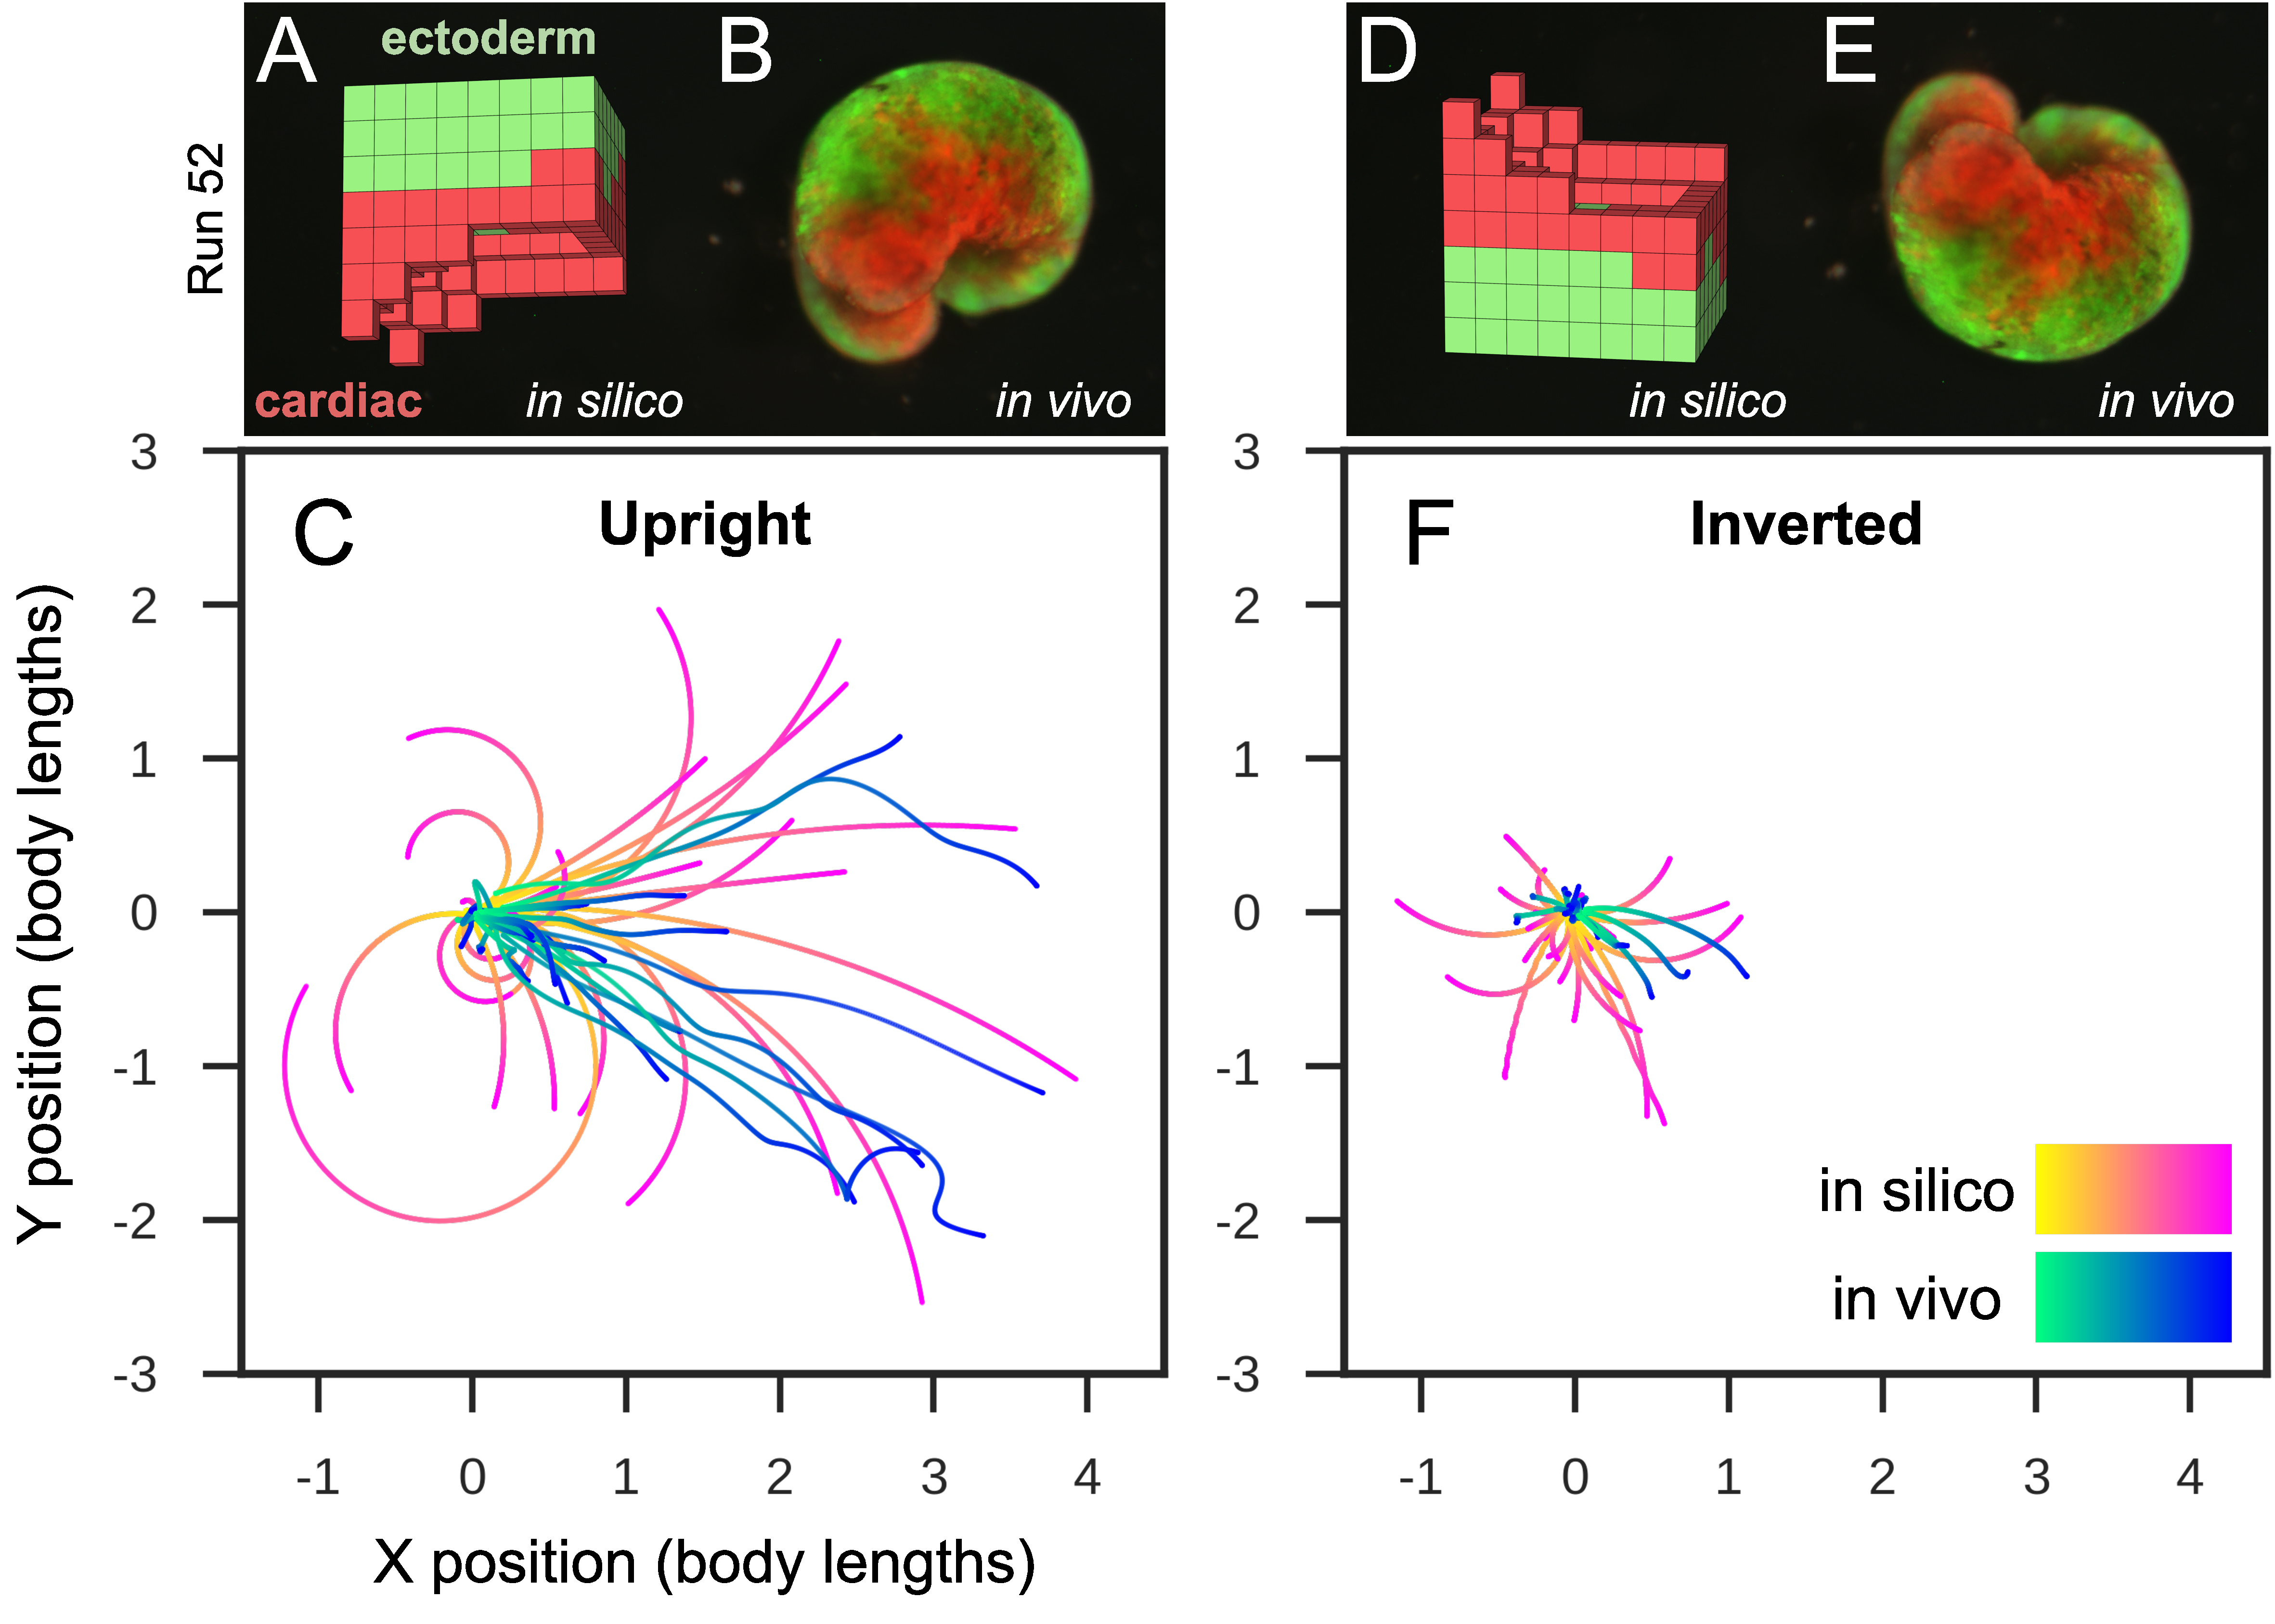
\includegraphics[width=\linewidth]{Chapter04/Fig4}
\caption{\label{fig-correlation}\textbf{Differential canalization.} 
Developmental windows (i.e.~the total lifetime developmental change) for morphology, $W_L$ (see Equation \ref{eq-WL}), and controller, $W_{\Phi}$ (see Equation \ref{eq-WPhi}), alongside fitness $F$.
(A) Three representative lineages taken from Supplementary Fig. \ref{fig:S1}, % S1, 
which displays the lineages of all 30 Evo-Devo run champions. Evolutionary time $T$ moves from the oldest ancestor (left) to the run champion (right). A general trend emerges wherein lineages initially increase their morphological development in $T$ (rising red curves) and subsequently decrease morphological development to almost zero (falling red curves). Five of the 30 evolutionary trials, annotated by {\Large $\ast$}, fell into a local optima.
(B) Median fitness as a function of morphology and controller development windows $(W_L,\; W_{\Phi})$, for all Evo-Devo designs evaluated. 
Overall, the fastest designs tend to have small amounts of morphological development, but are free to explore alternative control policies.}
\end{figure}

\begin{figure}[t]
\centering
\includegraphics[width=\linewidth]{Chapter04/Fig5}
\caption{\label{fig-random-walks}\textbf{Sensitivity to morphological and control mutations.}
Ten random walks were taken from each run champion.
(A) Successive \textit{control} mutations to the Evo and Evo-Devo run champions.
(B) The previous Evo-Devo results separately for fast and slow design types.
(C) Successive \textit{morphological} mutations to the Evo and Evo-Devo run champions.
(D) The previous Evo-Devo results separately for fast and slow design types. Medians plotted with 99\% confidence intervals.
The faster Evo-Devo robots tend to possess body plans that are robust to control mutations.}
\end{figure}

\begin{figure}[t]
\centering
\includegraphics[width=0.9\linewidth]{Chapter04/Fig6}
\caption{\label{fig-discovery}\textbf{Late onset discoveries.} Ontogenetic time before the discovery of rolling over, taken from the lineages of the best robot from each of the 25 Evo-Devo trials that produced a rolling design. Median time to discovery, with 95\% C.I.s, for (A) the lineage from the most distant ancestor $(T=0)$ to more recent descendants, and (B) the first ancestor to roll over compared to the final run champion. 
Rolling over is measured from the first time step the top of the robot touches the ground, rather than after completely rolling over. 
The first ancestors to roll over tend to do so at the end of their lives, their descendants tend to roll sooner in life, and the final run champions all begin rolling immediately at birth. 
These results are a consequence of dependent time steps: 
because mutational changes affect all downstream steps, their phenotypic impact is amplified in all but the terminal stages of development. Thus, late onset changes can provide exploration in the search space without breaking rest-of-life functionality, and subsequent evolution can gradually assimilate this trait to the start of development.}
\end{figure}


\section{Results}
\label{sec4:results}

We consider a locomotion task, over flat terrain, for soft robots composed of a $4\times4\times3$ grid of voxels (Fig. \ref{fig:blueprint}).
Robots are evaluated for 40 actuation cycles at 4 Hz, yielding a lifetime of ten seconds. Fitness is taken to be distance traveled measured in undeformed body lengths (four unit voxels, i.e.~4 cm). 
Example robots are shown in Figures \ref{fig:blueprint} and \ref{fig:trot-gallop-roll}, and Supplementary \href{https://youtu.be/Ee2sU-AZWC4}{\color{blue}Video S1}.


All experiments were performed in the open-source soft-body physics simulator  
\textit{Voxelyze} \cite{hiller2014dynamic}. 
Voxelyze simulates soft materials using two elements: particles and beams. 
A particle is a point mass with rotational inertia.
% Two adjacent particles are connected by a spring-like beam, which has translational and rotational stiffness.
A spring-like beam (with translational and rotational stiffness) connects two adjacent particles.
Each particle is connected to at most six neighbors (above, below, front, back, left, and right), on a cartesian grid.
Local material properties are stored at particles and averaged across shared beams.
Finally, a voxel mesh is drawn around each particle for visualization, such that adjacent voxels touch at the center of their shared beam.
More details about how this is actually implemented are given by Hiller and Lipson \cite{hiller2014dynamic}.

The morphology of a robot is given by the resting (beam) length stored at each voxel (Fig. \ref{fig:blueprint}).
However the shape and volume of each voxel is changed by external forces from the environment and internal forces via behavior. 
The morphology of a robot is denoted by the $4\times4\times3=48$-element vector $\ell$, where each element is the resting length stored at that voxel (with possible values within $1.0 \pm 0.75\; \text{cm}$).
Like most animals, our robots are bilaterally symmetrical.
We built this constraint into our robots because bilateral symmetry is known to help with forward locomotion
\cite{grabowsky1994symmetry}.
The lefthand $2\times4\times3=24$ resting voxel lengths are reflected on the other, righthand side of the midsagittal line, yielding 24 independent resting lengths.

The controller, however, is not constrained to be symmetrical since many behaviors, even for symmetric morphologies, consist of asymmetric gaits, and is given by the phase offset of each voxel from a global oscillating signal with an amplitude of 0.14 cm. 
The controller is denoted by the 48-element vector $\phi$, where each element is the phase offset of that voxel (with possible values within $0 \pm \pi/2$). 


We investigated the impact of development in this model by comparing two experimental variants: Evo and Evo-Devo (schematized in Supplementary Fig. \ref{fig:S2}). % \hyperref[fig:S2]{S2}). 
The control treatment, \textbf{Evo}, lacks development and therefore maintains a fixed morphology and control policy in a robot as it behaves over its lifetime. 
Two parameters per voxel are sufficient to specify an evolved robot at any time $t$ in its lifetime: its morphology $\ell_k$, and controller $\phi_k$.
An evolutionary algorithm optimizes 24 morphological and 48 control parameters.

The experimental treatment \textbf{Evo-Devo} evolves a developmental program rather than a static phenotype (Fig. \ref{fig:blueprint}). 
For each parameter in an Evo robot, an Evo-Devo robot has two: its starting and final value.
The evolutionary algorithm associated with the Evo-Devo treatment thus optimizes 48 morphological and 96 control parameters.
The morphology and controller of the $k$-th voxel change linearly from starting to final values, throughout the lifetime of a developing robot.
The endpoint parameters are denoted by asterisks: the controller develops from $\phi$ to $\phi^*$, the morphology develops from $\ell$ to $\ell^*$.
The starting and final points of development are predetermined by a genome which in turn fixes the direction (compression or expansion) and rate of change for each voxel.
Development is thus \textit{ballistic} in nature rather than adaptive, as it cannot be influenced by the environment (Equation \ref{eq4:ballistic-devo}). 


For both treatments we conducted 30 independent evolutionary trials.
At the end of evolutionary optimization, the non-developmental robots (Evo) tend to move on average with a speed of 10 body lengths in 10 seconds, or 1 length/sec. The evolved and developing robots (Evo-Devo) tend to move at over 5 lengths/sec (Fig. \ref{fig-fitness}A).
To ensure evolved and developing robots are not exploiting some unfair advantage conferred by changing body plans and control policies unavailable to non-developmental robots, we manually remove their development by setting $\ell^*=\ell$ and $\phi^*=\phi$, which fixes the structure of their morphologies and controllers at birth ($t=0$) (Equation \ref{eq4:ballistic-devo}). 
That is to say, we convert the evolved Evo-Devo robots into Evo robots (Equation \ref{eq4:ballistic-devo} reduces to Equation \ref{eq4:no-devo}).
The resulting reduced robots suffer only a slight (and statistically non-significant) decrease in median speed and still tend to be almost five times faster than the systems evolved without development (Fig. \ref{fig-fitness}B, treatment `Evo-Devo removed').
Ballistic development is therefore beneficial for search but does not provide a behavioral advantage in this task environment.


To investigate this apparent search advantage, we trace development and fitness across the 30 lineages which produced a `run champion': the robot with highest fitness at the termination of a given evolutionary trial (Supplementary Fig. \ref{fig:S1}).% \hyperref[fig:S1]{S1}). 
We measure the amount of ballistic change in each robot|its `ballistic plasticity'|by a statistic we call the \textit{developmental window}.
The developmental window is defined separately for morphology (Equation \ref{eq-WL}) and control (Equation \ref{eq-WPhi}) as the absolute difference in starting and final values summed across the robot and divided by the total amount of possible development, such that 0 and 1 indicate no and maximal developmental change, respectively.
Evo robots by definition have development windows of zero, as do Evo-Devo robots that have had development manually removed.
An Evo-Devo robot with a small developmental window has thus become \textit{canalized} \cite{waddington1942canalization}.


In terms of fitness, there were two observed basins of attraction in average velocity: a slower design type which either trots or gallops at a speed of less than 1 length/sec (Fig. \ref{fig:trot-gallop-roll}A,B and Fig. \ref{fig-correlation}A{\Large$\ast$}), and a faster design type that rolls at 5-6 lengths/sec (Fig. \ref{fig:trot-gallop-roll}C). 
After ten thousand generations, 25 out of a total of 30 Evo-Devo trials (83.3\%) find the faster design, compared to just 6 out of 30 Evo trials (20\%).


\subsection*{Differential canalization.}

Modular systems are more evolvable than non-modular systems because they allow evolution to improve one subsystem without disrupting others \cite{wagner1996perspective,lipson2007principles}.
Modularity may be a property of the way a system is built, or it may be an evolved property.
The robots evolved here are by definition modular because the genes which affect morphology are independent of those which affect its control.
However the more successful Evo-Devo lineages evolved an additional form of modularity, which we term differential canalization:
Some initially developmentally plastic traits become integrated and canalized, while other traits remain plastic.


In the successful Evo-Devo trials, morphological traits were canalized while control traits were not.
Evidence for this is provided in Supplementary Fig. \ref{fig:S1},%\hyperref[fig:S1]{S1}, 
which is summarized by Fig. \ref{fig-correlation}A.
Trajectories of controller development (green curves) do not follow any discernible pattern in phylogenetic time, and appear upon visual inspection to be consistent with a random walk or genetic drift.
The trajectories of morphological development (red curves), however, follow a consistent pattern.
The magnitude of morphological development increases slightly, but significantly $(p<0.001)$, before decreasing all the way to the most recent descendant, which is the most fit robot from that trial (the run champion). 
Run champions tend to have much less morphological development than their most distant ancestor $(p<0.001)$, but there is not a significant difference between champion and ancestral controller windows.
Furthermore, this pattern tends to correlate with high fitness: in trials in which this pattern did not appear (runs 6, 8, 16-18), fitness did not increase appreciably over evolutionary time.

This process within the lineages of the run champions is consistent with a more general correlation found in all designs explored during optimization across all runs: Individuals with the highest fitness values tend to have very small amounts of morphological development, while their control policies are free to develop (Fig. \ref{fig-correlation}B).
However, despite the fact that morphological development tends to be canalized in the most fit individuals, it cannot simply be discarded as the non-developmental systems have by definition small morphological windows, and small controller windows, but also low fitness.  


To test the sensitivity of the evolved morphologies to changes in their control policies, we applied a random series of control mutations to the Evo and Evo-Devo run champions from each evolutionary trial.
For each run champion, we perform 1000 subsequent random controller mutations that build upon each other in series (a Brownian trajectory in the space of controllers)|and repeat this process ten times for each run champion, each with a unique random seed.
It was found that optimized Evo-Devo robots tend to possess body plans that are much more robust to control mutations than those of Evo robots (Fig. \ref{fig-random-walks}A).
The first control mutation to optimized Evo robots tends to immediately render them immobile, whereas optimized Evo-Devo robots tend to retain most of their functionality even after 1000 successive random changes to their controllers.
Within Evo-Devo designs, the functionality of the 25 fast designs are minimally affected by changes to their control, whereas the five slow designs also tend to break after the first control mutation (Fig. \ref{fig-random-walks}B). 
Thus it can be concluded that these five robots are non-modular: their non-canalized morphologies evolved a strong dependency on their controllers. 
The Evo robots are similarly non-modular: they are brittle to control mutations. 


To test the sensitivity of the evolved controllers to changes in their morphologies, we applied the same procedure described in the previous paragraph but with random morphological mutations rather than control mutations.
It was found that both developmental and non-developmental systems tend to evolve controllers that are very sensitive to morphological mutations (Fig. \ref{fig-random-walks}C).
These findings are consistent with those of Cheney \textit{et al.} \cite{cheney2017scalable}, who also reported that robots were more sensitive to changes in their morphology than in their controllers.
Here, the first few morphological mutations to optimized robots, in both treatments, tend to immediately render them immobile.
Within Evo-Devo design types, neither of which canalized development in their controllers (Supplementary Fig. \ref{fig:S1},% \hyperref[fig:S1]{S1}), 
both the fast and slow designs possess controllers sensitive to changes in their morphologies (Fig. \ref{fig-random-walks}D).
Thus it can be concluded that the non-canalized controllers evolved a strong dependency on their morphologies. 
Therefore the only trait to be successfully canalized was also the only trait that rendered the agent robust to changes in other traits.



\subsection*{Heterochrony in morphological development.}


The evolutionary algorithm can rapidly discover an actuation pattern that elicits a very small amount of forward movement in these soft robots regardless of the morphology. 
There is then an incremental path of increasing locomotion speed that natural selection can climb by gradually growing legs to reduce the surface area touching the floor and thus friction, and simultaneously refining controller actuation patterns to better match and exploit the morphology (Fig. \ref{fig:trot-gallop-roll}A,B).


There is, however, a vastly superior design partially hidden from natural selection---a `needle in the haystack', to use Hinton and Nowlan's metaphor \cite{hinton1987learning}.
On flat terrain, rolling can be much faster and more efficient than walking, but finding such a design is difficult because the fitness landscape is deceptive.
Rolling over once is much less likely to occur in a random individual than shuffling forwards slightly. And as a population continues to refine walking morphologies and gaits, lineages containing rocking individuals which are close to rolling over, or roll over just once, do not survive long enough to eventually produce a true rolling descendant. 

Development can alter the search space evolution operates in because individuals sweep over a continuum of phenotypes, with different velocities, rather than single static phenotype that travels at a constant speed (Supplementary Fig. \ref{fig:S2}E,J).% \hyperref[fig:S2]{S2}E,J).
The lineages which ultimately evolved the faster rolling design initially increased their morphological plasticity in phylogenetic time as evidenced by the initial upward trends in the red curves in Supplementary Fig. \ref{fig:S1}% \hyperref[fig:S1]{S1} 
(summarized by Fig. \ref{fig-correlation}A) which contain a statistically significant difference between their starting and maximum developmental window sizes $(p<0.001)$.
This exposes evolution to a wider range of body plans and thus increases the chance of randomly rolling at least once at some point during the evaluation period.

The peak of morphological plasticity in  Supplementary Fig. \ref{fig:S1}% \hyperref[fig:S1]{S1}
(summarized by Fig. \ref{fig-correlation}A) generally lines up with the start of an increasing trend in fitness (blue curves) and marks the onset of differential canalization.
Rolling just once allows an individual to move further (1 body length) than some early walking behaviors but they incur the fitness penalty of having fallen over and thus not being able to subsequently walk for the rest of the trial. 
Therefore this tends to happen at the very end of ontogeny (Fig. \ref{fig-discovery}), as individuals evolve to `dive' in the last few time steps of the simulation of their behavior, thus incurring an additional increase of fitness over their parent, which does not exhibit this behavior.
Since more rolling incurs more fitness than less rolling, a form of progenesis occurs as heterochronic mutations move $\ell_k$ closer to $\ell_k^*$, for each voxel.
This gradually earlifies rolling from a late onset behavior to one that arises increasing earlier in ontogeny (Supplementary \href{https://youtu.be/Ee2sU-AZWC4}{\color{blue}Video S1}).
As more individuals in the population discover and earlify this rolling behavior, the competition stiffens until eventually individuals which are not born rolling from the start are not fast enough to compete (Fig. \ref{fig:trot-gallop-roll}C,D).


\subsection*{Generality of results.}


For the results above, as in nature \cite{lynch2010evolution}, the mutation rate of each voxel was left under evolutionary control (self-adaptation).
In an effort to assess the generality of our results, we replicated the experiment described above for various fixed mutation rates (Supplementary Fig. \ref{fig:S3}).% \hyperref[fig:S3]{S3}).
Without development, as in Hinton and Nowlan's case\cite{hinton1987learning}, the search space has a single spike of high fitness. 
One can not do better than random search in such a space.
At the highest mutation rate, optimizing Evo morphologies reduces to random search, and this is the only mutation rate where Evo does not require significantly more generations than Evo-Devo to find the faster design. 
This can be observed in Supplementary Fig. \ref{fig:S3}  % \hyperref[fig:S3]{S3} 
by comparing the generation at which the slopes of the fitness curves increase dramatically. 
However, the best two treatments, as measured by the highest median speed at the end of optimization, have development, and the robots they produced are significantly faster than those produced by random search (Evo with the highest mutation rate) $(p<0.01)$.

To further test the sensitivity of our results to the various settings of our particular system,
we transcribed the main experiment for a different class of morphologies (rigid bodies) and controllers (neural networks).
Details are provided in Supplementary Fig. \ref{fig:S5} %\hyperref[fig:S5]{S5} 
and Supplementary Methods.
The results of this test indicate that differential canalization exists elsewhere, but it does not always increase evolvability.  




\section*{Discussion}
\label{sec:discussion}

 
In these experiments, the intersection of two time scales|slow linear development and rapid oscillatory actuation, as from a central pattern generator|generates positive and negative feedback in terms of instantaneous velocity: the robot speeds up and slows down during various points in its lifetime (Supplementary Fig. \hyperref[fig:S2]{S2}J).
Prior to canalization, unless all of the phenotypes swept over by an individual in development keep the robot motionless, there will be intervals of relatively superior and inferior performance.
Evolution can thus improve overall fitness in a descendant by lengthening the time intervals containing superior phenotypes and reducing the intervals of inferior phenotypes. However, this is only possible if such mutations exist.

We have found here that such mutations do exist in cases where evolutionary changes
to one trait do not disrupt the successful behavior contributed
by other traits.
For example,
robots that exhibited the locally optimal trotting behavior 
(Fig. \ref{fig:trot-gallop-roll}A)
exhibited a tight coupling between morphology and control, and thus evolution was 
unable to canalize development in either one, since mutations to one subsystem 
tended to disrupt the other.
Brief ontogenetic periods of rolling behavior 
(Fig. \ref{fig:trot-gallop-roll}C), 
on the other hand, could be temporally extended by evolution through canalization of the morphology alone
(Fig. \ref{fig:trot-gallop-roll}D), 
since these morphologies are generally robust to the pattern of actuation.
The key observation here is that only phenotypic traits that render the agent robust to changes in other traits become assimilated, a phenomenon we term differential canalization. 

This insight was exposed by modeling the development of simulated robots as they interacted with a physically realistic environment.
Differential canalization may be possible in disembodied agents as well, 
if they conform to appropriate conditions described in Supplementary Discussion.

This finding of differential canalization has important implications for the evolutionary design of artificial and embodied agents such as robots.
Computational and engineered systems generally maintain a fixed form as they behave and are evaluated.
However, these systems are also extremely brittle when confronted with slight changes in their internal structure, such as damage, 
or in their external environment such as moving onto a new terrain
\cite{french1999catastrophic,
carlson2005ugvs,
bongard2006resilient}.
Indeed, a perennial problem in robotics and AI is finding general solutions which perform well in novel environments 
\cite{koos2013transferability,
nguyen2015deep
}.
Our results demonstrate how incorporating morphological development in the optimization of robots can reveal, through differential canalization, characters which are robust to internal changes.
Robots that are robust to internal changes in their controllers may also be robust to external changes in their environment \cite{bongard2011morphological}.
Thus, allowing robots to change their structure as they behave might facilitate evolutionary improvement of their descendants, even if these robots will be deployed with static phenotypes or in relatively unchanging environments.

These results are particularly important for the nascent field of soft robotics in which engineers cannot as easily presuppose a robot's body plan and optimize controllers for it because designing such machines manually is unintuitive
\cite{lipson2014challenges, pfeifer2012challenges}.
Our approach addresses this challenge, because differential canalization provides a mechanism whereby static yet robust soft robot morphologies may be automatically discovered using evolutionary algorithms for a given task environment.
Furthermore, future soft robots could potentially alter their shape to best match the current task by selecting from previously trained and canalized forms.
This change might occur pneumatically, as in Shepherd \textit{et al.} \cite{shepherd2011multigait}, or it could modulate other material properties such as stiffness (e.g.~using a muscular hydrostat).

We have shown that 
for canalization to occur in our developmental model, some form of paedomorphosis must also occur. However, there are at least two distinct methods by which such heterochrony can proceed: progenesis and neoteny.
Progenesis 
% |the acceleration of developmental processes such that adult traits of ancestors are realized earlier in juvenile stages of descendants| 
could occur through mutations which move initial parameter values $(\ell,\, \phi)$ toward their final values $(\ell^*,\, \phi^*)$.
Neoteny 
% |the retention of juvenile traits into the adult form as a result of retardation of development| 
could instead occur through mutations which move final values $(\ell^*,\, \phi^*)$ toward their initial values $(\ell,\, \phi)$.
Although a superior phenotype can materialize anywhere along the ontogenetic timeline, late onset mutations are less likely to be deleterious than early onset mutations.
This is because our developmental model is linear in terms of process, and interfering with any step affects all temporally-downstream steps. 
Since the probability of a mutation being beneficial is inversely proportional to its phenotypic magnitude \cite{fisher1930genetical}, mutational changes in the terminal stages of development require the smallest change to the developmental program.
Hence, late-onset discoveries of superior traits are more likely to occur without breaking functionality at other points in ontogeny, and these traits can become canalized by evolution through progenesis: mutations which reduce the amount of ontogenetic time prior to realizing the superior trait (by moving $\ell \rightarrow \ell^*$ and/or $\phi \rightarrow \phi^*$). 
Indeed progenesis was observed most often in our trials (Fig. \ref{fig-discovery}): late onset mutations which transform a walking robot into a rolling one are discovered by the evolutionary process, and are then moved back toward the birth of the robots'
descendants through subsequent mutations.

Finally, we would like to note the observed phenomenon of \textit{increased} 
% phenotypic 
% ballistic
plasticity prior to genetic assimilation.
Models of the Baldwin effect usually assume that phenotypic plasticity itself does not evolve, although it has been shown how major changes in the environment can select for increased plasticity in a character that is initially canalized \cite{lande2009adaptation}.
In our experiments however, there is no environmental change.
There is also a related concept known as `sensitive periods' of development in which an organism's phenotype is more responsive to experience 
\cite{bateson1979sensitive}.
Despite great interest in sensitive periods, the adaptive reasons why they have evolved are unclear \cite{Fawcett2015}.
In our model, increasing the amount of morphological development increases the chance of capturing an advantageous static phenotype, which can then be canalized, once found.
However, a phenotype will not realize the globally optimal solution by simply maximizing development.
This would merely lengthen the \textit{line} on which development unfolds in phenotypic hyperspace ($n$-dimensional real space).


The developmental model described herein is intentionally minimalistic in order to isolate the effect of morphological and neurological change in the evolutionary search for embodied agents.
The simplifying assumptions necessary to do so make it difficult to assess the biological implications.
For example, we model development as an open loop process 
and thus ignore environmental queues and sensory feedback 
\cite{Moczekrspb20110971,snell2013overview}.
We also disregard the costs and constraints of phenotypic plasticity 
\cite{snell2012selective,murren2015constraints}. 
By removing these confounding factors, we hope these results will help generate novel hypotheses about morphological development, heterochrony, modularity and evolvability in biological systems.




\section{Methods}
\label{sec4:methods}


\subsection*{Ballistic development.}

Ballistic development 
$\mathcal{B}(t)$
is simply a linear function from a starting value $a$ to a final value $b$, in ontogenetic time $t\in(0,\tau)$, thus: 
\begin{equation}
\label{eq4:ballistic-devo}
\mathcal{B}(t) = a + \frac{t(b-a)}{\tau}.
\end{equation}
For Evo robots, $a=b$, hence:
\begin{equation}
\label{eq4:no-devo}
\mathcal{B}(t) = a,
\end{equation}
which is just a constant value in ontogenetic time.

Because $a$ and $b$ are constants set by the genotype and $\tau=10$ (sec) is a fixed hyperparameter, development is predetermined, monotonic and irreversible|in a word: ballistic.



\subsection*{Current length.} 

For smaller voxels, it is necessary to implement damping into their actuation to avoid simulation instability. 
Actuation amplitude is limited by a linear damping factor $\xi(x) = \min\{1,\, (4x-1)/3\}$, which only affects voxels with resting length less than one centimeter, and approaches zero (no actuation) as the resting length goes to its lower bound of 0.25 cm.
% \begin{equation}
% \xi(x) = \min \left(1,\quad \frac{4x-1}{3}\right) =
% \begin{cases} 
%       1 & 1 \leq x \leq \frac{7}{4}  \\
% %       (4x-1)/3 & x < 1
%       \frac{4x-1}{3} & \frac{1}{4} \leq x < 1
%    \end{cases}
% \end{equation}

Actuation of the $k$-th voxel $\psi_k(t)$ therefore depends on the starting and final phase offsets $(\phi_k,\, \phi_k^*)$ for relative displacement, and on the starting and final resting lengths $(\ell_k,\, \ell_k^*)$ for amplitude. With maximum amplitude $A=0.14$ cm and a fixed frequency $f=4$ Hz, we have:
\begin{equation}
\label{eq-actuation}
\psi_k(t) = A \cdot \sin\left[2\pi f t + \phi_k + \frac{t(\phi_k^*-\phi_k)}{\tau}\right] \cdot \xi\left[\ell_k + \frac{t(\ell_k^*-\ell_k)}{\tau}\right]
\end{equation}
The current length of the $k$-th voxel at time $t$, denoted by $\mathcal{L}_k(t)$, is the resting length plus the offset and damped signal $\psi_k(t)$.
\begin{equation}
\label{eq-curr-length}
\mathcal{L}_k(t) = \ell_k + \frac{t(\ell_k^*-\ell_k)}{\tau} + \psi_k(t)
\end{equation}
Current length is broken down into its constituent parts for a single 
% (undamped) 
voxel, under each treatment, in Supplementary Fig. \ref{fig:S2}.% \hyperref[fig:S2]{S2}.



\subsection*{Evolutionary algorithm.}

We employed a standard evolutionary algorithm, Age-Fitness-Pareto Optimization \cite{schmidt2011age}, which uses the concept of Pareto dominance and an objective of age (in addition to fitness) intended to promote diversity among candidate designs. 
\textit{A single evolutionary trial maintains a population of thirty robots, for ten thousand generations.}
Every generation, the population is first doubled by creating modified copies of each individual in the population.
The age of each individual is then incremented by one.
Next, an additional random individual (with age zero) is injected into the population (which now consists of 61 robots). 
Finally, selection reduces the population down to its original size (30 robots) according to the two objectives of fitness (maximized) and age (minimized).

We performed the above procedure thirty times to produce \textit{thirty independent evolutionary trials.}
That the number of trials is the same as the population size within each trial is an admittedly confusing coincidence.

The mutation rate is also evolved for each voxel, independently, and slightly modified every time a genotype is copied from parent to child.
These 48 independent mutation rates are initialized such that only a single voxel is mutated on average.
Mutations follow a normal distribution $(\sigma_{\ell}=0.75$ cm; $\sigma_{\phi}=\pi/2)$ and are applied by first selecting what parameter types to mutate $(\phi_k,\, \phi_k^*,\, \ell_k,\, \ell_k^*)$, and then choosing, for each parameter separately, which voxels to mutate. 
In Supplemental Materials we provide exact derivations of the expected genotypic impact of mutations, in terms of the proportions of voxels and parameters modified, for a given fixed mutation rate $\lambda$.
There is a negligible difference between Evo and Evo-Devo in terms of the expected number of parent voxels modified during mutation (Supplementary Fig. \ref{fig:S4}).% \hyperref[fig:S4]{S4}).
% Empirically, there was not a statistically significant difference in the number of voxels mutated between Evo and Evo-Devo samples.


\subsection*{Developmental windows.}

The amount of development in a particular voxel can range from zero (in the case that starting and final values are equal) to 1.5 cm for the morphology (which ranges from 0.25 cm to 1.75 cm) and $\pi$ for the controller (which ranges from $-\pi/2$ to $\pi/2$). 
The morphological development window, $W_L$, is the sum of the absolute difference of starting and final resting lengths across the robot's 48 voxels, divided by the total amount of possible morphological development.
\begin{equation}
W_L = \frac{1}{48(1.5)} \sum_{k=1}^{48} |\ell^*_k-\ell_k|
\label{eq-WL}
\end{equation}
The controller development window, $W_{\Phi}$, is the sum of the absolute difference of starting and final phase offsets across the robot's 48 voxels, divided by the total amount of possible controller development. 
\begin{equation}
W_{\Phi} = \frac{1}{48\pi} \sum_{k=1}^{48} |\phi^*_k-\phi_k|
\label{eq-WPhi}
\end{equation}


\subsection*{Statistical hypothesis testing.}

We used the Mann-Whitney $U$ test to calculate the $p$-values reported in this paper.


\subsection*{Data availability.}

\href{https://github.com/skriegman/how-devo-can-guide-evo}{\color{blue}\textbf{github.com/skriegman/how-devo-can-guide-evo}} contains the source code necessary for reproducing the results reported in this paper.


% \begin{itemize}

% \item[{\Large$\star$}]
% \href{https://github.com/skriegman/how-devo-can-guide-evo}{\textbf{https://github.com/skriegman/how-devo-can-guide-evo}} contains the source code necessary for reproducing the results reported in this paper.

% % \item 
% % \href{https://github.com/skriegman/evosoro}{\textbf{https://github.com/skriegman/evosoro}} is a more general repository to fork which provides additional examples in different environments and with various evolutionary tool sets.

% \end{itemize}




% \section{Supplementary Video}
\subsection*{Supplementary Video S1.}
\label{video}
\href{https://youtu.be/Ee2sU-AZWC4}{\color{blue}\textbf{youtu.be/Ee2sU-AZWC4}}
provides a high-level overview of the results reported in this paper.





\section{Supplementary Discussion}
\label{sec4:supplementary-discussion}



\subsection*{Embodiment.}

We consider an agent to be embodied if its output affects its input.
This relationship may be represented by the simple update rule $\ell_{t+1} = f(\ell_t,\, \phi)$,
where $\ell_t$ denotes the morphology of an agent at time $t$, and $\phi$ denotes its control policy.
In a disembodied system, changes to the morphology are not directly constrained by its current state; the update rule becomes: $\ell_{t+1} = f(\phi)$.

Once a round robot begins rolling, its control policy cannot instantaneously force the system to go in the other direction, since
momentum will tend to preserve forward movement.
This has the effect of reducing selection pressure on the controller, since fewer variations are deleterious.
This allows evolution to continue climbing fitness gradients by mutating the controllers within these permissive body plans.

This might also be possible in disembodied agents if other dimensions of the system can be changed by some search process such as to facilitate the search for $\phi$.



\section{Supplementary Methods}
\label{sec4:supplementary-methods}

\subsection*{Rigid-bodied robots.}

Rigid-bodied robots and their environment were simulated using Pyrosim
(\href{https://ccappelle.github.io/pyrosim/}{\color{blue}ccappelle.github.io/pyrosim}).
% \cite{kriegman2017simulating}.
The robot is a quadruped with a large, spherical abdomen; each leg is attached by a single degree-of-freedom hinge joint.\\[0.75em]
\centerline{\includegraphics[width=0.4\linewidth]{Chapter04/rigid-body.png}}

\vspace{0.75em}
Morphological development was approximated in rigid bodies using linear actuators to slowly lengthen or shorten the length of each leg, from an evolved starting value (between 0 and 1) to an evolved final value (between 0 and 1).
The controller is a simple neural net: two central pattern generators are fully connected to four motor neurons, each of which innervate a separate hinge joint.
Controller development was approximated in neural networks through ballistic change to each synaptic weight: As the simulation proceeds, each weight develops linearly, from an evolved starting value (between -1 and +1) to an evolved final value (between -1 and +1).


The genotype spans two arrays: one for initial and final synaptic weights (controller), and another for initial and final leg lengths (morphology). 
Mutations affect, on average, a single element in each array.
Apart from the genotype and its mutations, the evolutionary algorithm is identical to that of the soft robots.
However, the task environment now consists of a sloped floor, declined toward a light source; and
performance is measured by the average light intensity recorded by a light sensor embedded in the center of the agent's abdomen, according to the inverse square law of light propagation, at each time step in its life. Occlusion of the light caused by interference of the robot's own body parts was not simulated.


The results are presented below in Supplementary Fig. \hyperref[fig:S5]{S5}.


\subsection*{Mutations for soft robots.}

The following derivation shows that there is a negligible difference in the mutations produced by the Evo and Evo-Devo treatments, in terms of the number of voxels modified (Fig. \hyperref[fig:S4]{S4}). 

Each voxel cell of a soft robot has its own material properties that can be changed by the evolutionary algorithm.
Evo voxels have two material properties: (1) resting length and (2) phase offset.
Evo-Devo voxels have four material properties: (1) initial resting length, (2) final resting length, (3) initial phase offset, and (4) final phase offset.


Mutations are applied by first choosing which material properties to mutate, and then choosing, separately for each property, which voxels to modify.
For each of the $n$ material properties, we select it with independent probability $p=1/n$. 
If none are selected, we randomly choose one. This occurs with probability $\left(1-p\right)^n$.
Hence the number of selected material properties for mutation is a random variable $S$ which follows a truncated binomial distribution,
\begin{equation}
\text{Pr}(S = s \mid n) = 
	\begin{cases} 
        0 & \text{ for } \;  s = 0 \\[4pt]
        n p(1-p)^{n-1} + (1-p)^n & \text{ for } \;  s = 1 \\[8pt]
        \dbinom{n}{s} p^s (1-p)^{n-s} & \text{ for } \;  s > 1
	\end{cases}
\end{equation}
The expected number of selected material properties is then:
\begin{align}
\mathbb{E}(S) 
&=
np(1-p)^{n-1} + (1-p)^n + \sum_{s=2}^n s \binom{n}{s} p^s (1-p)^{n-s} \\
&= 
(1-p)^n + \sum_{s=1}^n s \binom{n}{s} p^s (1-p)^{n-s} \\
&= 
(1-p)^n + np \\
&= 
(1-p)^n+1 .
\end{align}


For a selected material property, 
each voxel is mutated independently with probability $\lambda$, a hyperparameter we call the \textbf{mutation rate}.
The expected \textit{number} of genotype elements mutated given $K$ total voxels is thus:
\begin{equation}
\delta_{\text{gene}} = \lambda K \cdot \mathbb{E}(S) .
\end{equation}
Dividing by the length of the genome, $nK$, we get the expected \textit{proportion} of genotype elements mutated:
\begin{equation}
\pi_{\text{gene}} = \lambda/n \cdot \mathbb{E}(S).
\end{equation}
Note that imposing bilateral symmetry does not change these expected values.

We have $K=48$ total voxels, and $n=\{2,4\}$ material properties for our two main experimental treatments \{Evo, Evo-Devo\}, respectively. The expected difference between a robot and its offspring, in terms of genotype elements, is summarized in the following table.
\vspace{-1em}
\begin{table}[!ht]
\centering
\begin{tabular}{rcc}
 & $n=2$ & $n=4$  \\ \cline{2-3} 
\multicolumn{1}{r|}{$\delta_{\text{gene}}$}     & \multicolumn{1}{c|}{$60\lambda$}    & \multicolumn{1}{c|}{$63.8175\lambda$} \\ \cline{2-3} 
\multicolumn{1}{r|}{$\pi_{\text{gene}}$} & \multicolumn{1}{c|}{$0.625\lambda$} & \multicolumn{1}{c|}{$0.3291\lambda$}  \\ \cline{2-3} 
\end{tabular}
\end{table}

\noindent
However, because multiple material properties can be mutated within a single voxel, the expected number of voxels mutated is lower than the expected number of genotype elements mutated. 
To calculate the average number of voxels mutated we need to consider a hierarchy of binomial distributions.


Given that $S$ material properties were selected for mutation,
the number of material properties mutated within a single voxel, $M$ follows a binomial distribution, 
% $M\sim\text{binom} (S, \lambda)$,
\begin{equation}
\text{Pr}(M=m \mid S, \lambda) 
= 
\dbinom{S}{m} \lambda^m (1-\lambda)^{S-m} .
\end{equation}
For brevity, let's denote the probability that at least one mutation occurs within the voxel as $\theta$,
\begin{equation}
\theta = \text{Pr}(M>0 \mid S,\lambda)
=
1-(1-\lambda)^S .
\end{equation}
Then the number of voxels mutated, $V$, across a total of $K$ voxels and $S$ selected material properties, also follows a binomial distribution:
% binom$(K, \theta)$. 
\begin{equation}
\text{Pr}(V=v \mid S, K, \lambda, n) 
= 
\dbinom{K}{v} \theta^v (1-\theta)^{K-v}.
\end{equation}
And the expected number of voxels mutated (out of $K$ total) is
\begin{align}
\delta_{\text{vox}}
&=
\mathbb{E}(V \mid K, \lambda, n) \\
&=
\mathbb{E}_S \, \mathbb{E}_{V}(V \mid S, K, \lambda, n) \\
&= 
\mathbb{E}_S (K\theta \mid S, K, \lambda, n) \\
&=
K \left\{
1-\mathbb{E}_S \left[(1-\lambda)^S \mid \lambda, n\right] \right\} \\
&=
K \left\{ 1 - \left[ (1-\lambda)(1-p)^n
+  \sum_{s=1}^{n} (1-\lambda)^s \dbinom{n}{s} p^s (1-p)^{n-s}
 \right] \right\} \\
&=
K \left\{ 
1 - (1-p)^n \left[ \left(\frac{\lambda p-1}{p - 1}\right)^n - \lambda\right]
\right\} 
\end{align}

 
There is an extremely tight bound on the proportion of voxels mutated, $\pi_{\text{vox}} = \delta_{\text{vox}}/K$, for any $n > 1$  (Fig. \hyperref[fig:S4]{S4}).
Thus mutations in Evo $(n=2)$ and Evo-Devo $(n=4)$ have practically the same impact in terms of the number of voxels modified.
For completeness, the following table displays $\delta_{\text{vox}}$ for the specific values of $\lambda$ considered by our hyperparameter sweep ($K=48$) (Fig. \hyperref[fig:S3]{S3}). 
\vspace{-0.5em}
\begin{table}[h!]
\centering
\begin{tabular}{cccccccccc}
  & & \multicolumn{8}{c}{$\lambda$} \\ \cline{3-10}
  & \multicolumn{1}{c|}{}  & 1/48    & 2/48    & 4/48    & 8/48    & 16/48   & 24/48   & 32/48   & \multicolumn{1}{c|}{48/48} \\ \cline{2-10} 
\multicolumn{1}{c|}{\multirow{2}{*}{$n$}} & \multicolumn{1}{c|}{2} &
1.25 & 2.48 & 4.92 & 9.67 & 18.67 & 27 & 34.67 & \multicolumn{1}{c|}{48}    \\
\multicolumn{1}{c|}{}                     & \multicolumn{1}{c|}{4} & 
1.3 & 2.6 & 5.14 & 10.05 & 19.17 & 27.46 & 34.98 & \multicolumn{1}{c|}{48}    \\ \cline{2-10} 
\end{tabular}
\end{table}










\begin{figure}
\centering
\includegraphics[width=\linewidth]{Chapter04/FigS1}
\caption{\label{fig:S1}\textbf{Evolutionary change during 30 Evo-Devo trials.} The amount of morphological development, $W_L$ (see Equation 3), controller development, $W_{\Phi}$ (see Equation 4), and fitness, $F$, for the lineages of the 30 Evo-Devo run champions. Evolutionary time, $T$, moves from the oldest ancestor (left) to the run champion (right). A general trend emerges wherein lineages initially increase their morphological development in $T$ (rising red curves) and subsequently decrease morphological development to almost zero (falling red curves). Five of the 30 evolutionary trials, annotated by {\Large $\ast$}, fell into a local optima.}
\end{figure}



\begin{figure}
\centering
\includegraphics[width=0.6\linewidth]{Chapter04/FigS2}
\caption{\label{fig:S2}\textbf{Experimental treatments.} The phase of an oscillating global temperature (A, F) is offset in the $k$-th voxel by a linear function from $\phi_k$ to $\phi_k^*$ (B, G). 
The resting length of the $k$-th voxel is a linear function from $\ell_k$ to $\ell_k^*$ (C, H). 
For Evo, there is no development, so $\phi_k=\phi_k^*$ and $\ell_k=\ell_k^*$.
The offset actuation is added on top of the resting length to give the current length of the $k$-th voxel (D, I). 
These example voxel-level changes occur across ontogenetic time $(t)$, independently in each of the 48 voxels, and together interact with the environment to generate robot-level velocity (E, J).
To see this, we averaged displacement across intervals of two actuation cycles (0.5 sec) and plotted the smoothed velocities for two Evo-Devo run champions with minimal canalization (J) alongside their non-developmental counterparts (E).
Also note that the frequency of actuation is plotted here at 1.4 Hz; but, in our experiments, we used a frequency of 4 Hz.
}
\end{figure}




\begin{figure}
\centering
\includegraphics[width=\linewidth]{Chapter04/FigS3}
\caption{\label{fig:S3}\textbf{Mutation rate sweep.} 
Median fitness (with 95\% bootstrapped confidence intervals) under various mutation rates, $\lambda$, a hyperparameter defined in Supplementary Methods which affects the probability a voxel is mutated. 
In the main experiment of this paper, the mutation rate is evolved for each voxel independently, and is constantly changing.
In this mutation rate sweep, $\lambda$ is held uniform across all voxels.
There were two observed basins of attraction in terms of fitness: a slower design that trots/gallops 5-15 body-lengths during the evaluation period, and a faster design type that rolls at 50-70 body-lengths. 
Although higher mutation rates facilitate the discovery of the superior phenotype, once found, lower mutation rates tend to produce more refined and faster robots.
Without development, the search space has a single spike of high fitness. 
One can not do better than random search in such a space.
When $\lambda=1$, optimizing Evo morphologies reduces to random search, and this is the only mutation rate where Evo does not require significantly more generations than Evo-Devo to find the faster design type.
This can be observed for $\lambda\in\{1/6,\, 1/3,\, 1/2,\, 2/3,\, 1\}$, by comparing the generation at which the slopes of the fitness curves increase dramatically.
However, the best two treatments (Evo-Devo at $\lambda=1/2$ and $\lambda=2/3$), as measured by the highest median speed at the end of optimization, have development, and the robots they produced are significantly faster than those produced by random search (Evo with the highest mutation rate)
$(p<0.01)$.
}
\end{figure}



\begin{figure}
\centering
\includegraphics[width=0.5\linewidth]{Chapter04/FigS4}
\caption{\label{fig:S4}\textbf{Mutational impact.} The expected proportion of voxels modified, $\pi_{\text{vox}}$, where $n$ is the number of material properties that can be mutated, and $\lambda$ is the mutation rate.
A derivation is provided in Supplementary Methods.
Regardless of $n$,
when $\lambda=1$, every voxel must be mutated, and when $\lambda=0$, no voxels can be mutated. 
Between these two points, there is an extremely tight bound on the proportion of voxels mutated for any $n>1$. 
In this paper, we have treatments Evo, with $n=2$, and Evo-Devo, with $n=4$.
}
\end{figure}




\begin{figure}
\centering
\includegraphics[width=0.65\linewidth]{Chapter04/FigS5}
\caption{\label{fig:S5}\textbf{Differential canalization in rigid bodies.} 
This environment consists of a sloped floor, declined toward a light source. 
Rigid-bodied robots, which are described in Supplementary Methods, perform phototaxis.
Although longer legs produce faster walking behaviors, the shortest leg setting places the robot's large, spherical abdomen onto the ground, allowing the robot to simply roll down the ramp toward the light. 
An ancestor discovers rolling over toward the end of its evaluation period through ontogenetic morphological change that compresses leg lengths. 
This rollable morphology is assimilated to the start of development through differential canalization: The sooner a robot shrinks its legs, the sooner it can begin rolling; eventually descendants start with compressed legs, are able to immediately roll, exhibit little to no morphological change, but continue to sweep over many different synaptic weights as they behave. 
Rolling down the slope is not entirely passive, however, since protruding legs, even at their shortest setting, can slow down or even stop forward movement. 
The best controllers not only avoid such interference, but also guide rolling toward the light source. 
However, development in this particular case did not affect evolvability. 
These results are consistent with predictions made by other quantitative models used in theoretical biology that suggest that plasticity only expedites evolution under restrictive conditions \cite{ancel2000undermining}. 
We hypothesize that, in our case, this is because the search space is not deceptive enough: Once the rigid-bodied robot evolves to compress its legs, and touch its abdomen to the sloped floor, it will tend to roll for the remainder of its evaluation period.
That is, in contrast with the soft robots, there is no intermediate stage between walking and rolling that suffers the fitness penalty of no longer being able to move.
}
\end{figure}






% 

% \chapter{Environment-Mediated Development}
\chapter{Structure, Configuration, and Material}


\vspace{-2em}

{\footnotesize
\noindent
Appeared as:
S.~Kriegman et al., Interoceptive robustness through environment-mediated morphological development. \textit{Proceedings of the Genetic and Evolutionary Computation Conference} (2018).
}


\begin{figure}[!h]
    \centering
    \includegraphics[width=\linewidth]{Chapter06/img/Callosities} \\
    \vspace{-0.5em}
    \includegraphics[width=0.35\linewidth]{Chapter06/img/colorbar} \\
    % \vspace{-1em}
    \caption{A single robot grows calluses as it walks, 
    % selectively rigidifying
    in response to pressure on its feet   
    (\href{https://youtu.be/0cmwpcxSUWI}{\textbf{\texttt{youtu.be/0cmwpcxSUWI}}}).
    } % (The champion of run 6.)
    \label{fig:calluses}
    % \vspace{1em}
\end{figure}

\noindent
Typically, AI researchers and roboticists try to realize
intelligent behavior in machines by tuning parameters of a 
predefined structure (body plan and/or neural network
architecture) using evolutionary or learning algorithms. 
Another but not unrelated longstanding property of these systems is their brittleness to slight aberrations, as highlighted by the growing deep learning literature on adversarial examples.
Here we show robustness can be achieved by
evolving the 
geometry of soft robots, their
control systems, and how
their material properties develop
in response to one particular interoceptive stimulus
(engineering stress) during their lifetimes.
By doing so we realized robots that 
were equally fit but more robust to 
extreme material defects (such as 
might occur during fabrication or by damage thereafter)
than robots that did not develop during their lifetimes,
or developed in response to a different interoceptive
stimulus (pressure).
This suggests that the interplay between changes
in the containing systems
of agents (body plan and/or neural architecture)
at different temporal scales (evolutionary
and developmental) along different modalities
(geometry, material properties, synaptic weights)
and in response to different signals (interoceptive
and external perception) all
dictate those agents' abilities to evolve or 
learn capable and robust strategies. 


% \subsubsection*{Video playlist}

% Link: 
% \href{http://goo.gl/T5wZNQ}{\textbf{\texttt{goo.gl/T5wZNQ}}}

% Link: 
% \href{https://www.youtube.com/playlist?list=PL7qssg0uLKTaFhaCRC0WviaGeOitOE8MR}{\textbf{\texttt{youtube.com/playlist?list=PL7qssg0uLKTaFhaCRC0WviaGeOitOE8MR}}}


% \section{Introduction}
\label{sec6:introduction}

A major characteristic of life is that three broad time scales are relevant to it: evolution, development and physiological functioning.
% \citep{waddington1957strategy}.
Engineered systems, in marked contrast, often employ an evolutionary or learning algorithm to improve their behavior over time, but rarely employ morphological development; any changes to the physical layout are made in between evaluations \citep{sims1994evolving,lipson2000automatic,cheney2013unshackling}, if they are made at all.

Two notable exceptions are modular robots \citep{zykov2005robotics}, which may reconfigure their bodies by adding and removing discrete structures, and soft robots \citep{shepherd2011multigait}, which may continuously alter the local volumes of different parts of their
bodies while behaving. 
Others \citep{bongard2011morphological} have approximated topological change in rigid bodies by extending outward and angling downward 
appendages using a combination of linear and rotary actuators, thus simulating limb growth.

Several computational but embodied models of \textit{prenatal} development have been reported in the literature \cite{dellaert1996developmental,
% dellaert1994toward,
Eggenberger97,
Bongard01,
% bongard2003evolving,
miller2004evolving,
doursat2009organically}.
As implied,
cellular growth therein occurred prior to any physiological functioning. 
Thus, these studies included change during only
two of the three time scales relevant to life:
evolutionary and behavioral change, but not postnatal developmental
change.

The most common argument in favor of development is that some aspects of the environment are unpredictable, so it is advantageous to leave some decisions up to development rather than specifying them genetically.
Although self evident, it remains to determine which mechanisms of development should be instantiated in robots to realize plastic, adaptive, and useful machines.

Naturally, the performance of an evolved system depends on its capacity for evolutionary improvement: its evolvability.
Development can, under certain conditions, smooth the search space evolution that operates in, thus increasing evolvability.
This process, known as the Baldwin effect \citep{baldwin1896new,dennett2003baldwin}, starts with an advantageous characteristic acquired during the development of individuals, such as the callouses in Fig. \ref{fig6:calluses}. 
This can create a new gradient in the evolutionary search space, rewarding descendants that more rapidly manifest the trait during their lifetimes \citep{hinton1987learning,kriegman2018morphological}
and retain it through the remainder of their lifetime \citep{kriegman2017minimal}.
Assuming such mutations exist and can be naturally selected \citep{kriegman2018morphological}, following the gradient requires incrementally reducing development in the manifold of the search space that can express variations on the trait \cite{waddington1942canalization}.


However, fitness landscapes that evolution climbs, and development sometimes smooths, tend not to remain static in realistic settings.
On this vacillating landscape, when the best thing to do does not remain the same, a highly evolvable but non-robust system will need to keep starting over from scratch every time the conditions change.
Computational and engineered systems provide countless examples of systems with nearly perfect performance in a controlled environment, such as a factory, but who turn out to be (often comically) brittle to slight changes in their internal structure, such as damage, or their external environment such as moving on to new terrain or transferal from simulation to reality 
\citep{carlson2005ugvs,
koos2013transferability,
% mccloskey1989catastrophic,
% french1999catastrophic,
goodfellow2013empirical,
szegedy2013intriguing,
% goodfellow2014generative,
athalye2018synthesizing,
% gilmer2018adversarial,
% su2017one,
nguyen2015deep}.

Although generally absent from engineered systems (but see \cite{bongard2006resilient,cully2015robots}), the canonical form of robustness is seen to some extent in all organisms, and it comes from the act of development itself.
For example, a plant that grows according to a fixed program will capture less light than a plant that grows toward sunlight.
But there is another, more subtle form of robustness that we will refer to as `intrinsic robustness' because it is a property of a system's structure rather than of the process by which it may change.

Developmental change produces intrinsically robust systems because they evolved from designs that had to maintain adequate performance along additional dimensions of change \citep{bongard2011morphological,kriegman2018morphological}.
Through morphological development specifically, evolution is compelled to maintain designs that are capable across a series of body plans, with different 
% behavioral repercussions of action, and different 
sensor-motor contingencies; and the ability to tolerate such perturbations can become inherited to some extent in descendants' behaviors \cite{bongard2011morphological} and morphologies \cite{kriegman2018morphological}, even when their developmental flexibility is reduced or completely removed by canalization or fabrication.


And yet, despite the ubiquity of
% (postnatal) 
morphological development in nature, and the adaptive advantages it seemingly confers, there are only a handful of cases reported in the literature in which a simulated robot's mechanical structure was allowed to change while it was behaving 
(e.g.~\citep{ventrella1998designing,
komosinski2003framsticks,
bongard2011morphological,
kriegman2018morphological,
kriegman2017minimal}),
all of which modeled morphological development as a genetically predetermined process: the environment could not influence the way in which development unfolded. 


Assuming that an engineered system is capable of local morphological change in response to environmental signals, it is unclear how it should do so, beyond the examples of morphological plasticity observed in nature. 
Examples include Wolff's law \citep{ruff2006s}---bone grows in response to particular mechanical loading profiles---and Davis' law---soft tissue increases in strength in response to intermittent mechanical demands.
One can envisage other such laws that are not known to occur in biology but could be helpful in a specific artificial system, such as end effectors softening in response to pressure, which might enhance their ability to safely manipulate irregular or delicate objects \cite{brown2010universal}.
Indeed, the genesis of the work presented here is one such anecdotal example given in \citep{corucci2017evolutionary}, where a single robot, subjected to an abrupt doubling in gravity, stiffened its body in reaction to the increased pressure.
However, whether or how it could provide a behavioral advantage, nor whether pressure is the best interoceptive signal to developmentally respond to,
was not investigated.

As a step towards a more adequate picture, we introduce here a simple form of a developmental feedback mechanism:
Genetic systems dictate how organisms develop in response to interoceptive stimuli, and development alters the kinds of interoceptive conditions the organism experiences.
More specifically, at every time step, the proposed model of closed-loop development:
\begin{enumerate}
\item `listens to' load signatures generated from movement; and, in response,
\item modifies the robot's rigidity,
\end{enumerate}
which will change the way it distributes load and generates movement at the next time step.


Optimizing a system that may form a continuum of rigid and soft components---and in which this admixture may change over time---is extremely nonintuitive and underexplored.
Thus, a study of the adaptive properties of such systems---and how they can best be optimized to render useful work---is initiated here.



% \section{Methods}
\label{sec:methods}

We evolved locomotive machines constructed from voxels with heterogeneous stiffness. 
Like many organisms \citep{ruff2006s}, the robot's material stiffness progressively changes in response to mechanical loading incurred as the robot behaves.
This ontogenetic change occurs independently at each voxel according to an evolved local rule.


\subsection{Physical simulation.}

The soft-matter physics engine \textit{Voxelyze} \citep{hiller2014dynamic} is used to calculate the movement of robots resulting from their interaction with a virtual 3D terrestrial environment.
Each robot is simulated for 25 times the length of an expansion/contraction cycle (a total of five seconds). 
The displacement between the starting coordinates and the agent's final center of mass (in the $xy$ plane) is recorded.\footnote{\href{https://github.com/skriegman/2018-gecco}{\textcolor{blue}{\textbf{\texttt{github.com/skriegman/2018-gecco}}}} contains the source code necessary for reproducing the results reported in this paper.}


% For a more general purpose repository see \href{https://github.com/skriegman/evosoro}{\textcolor{blue}{\textbf{\texttt{github.com/skriegman/evosoro}}}}


\subsection{Heavy materials.}

% 1e6 -> 1e9 density
% vol = length^3
% mass = vol * density 
% previously each voxel was a centimeter in length and one gram in mass.
% now each voxel is 1 kg/cm^3 in mass, which is heavier than the heaviest material on earth (22 g/cm^3) so this calculation is incorrect. 

Materials are simulated to have increased mass relative to those used by \cite{hiller2012automatic,cheney2013unshackling,cheney2014electro}.
Constructed from heavier materials, many previously mobile robots become crushed under their own weight and require stiffer material to support locomotion with the same geometry.
However, we also restricted actuation amplitude as materials grow stiffer to better approximate the properties of real materials with different stiffnesses.
This creates an interesting and realistic trade-off: the stiffest material can easily support any body plan but cannot move on its own (like a skeleton without muscle), whereas the softest material can readily elicit forward movement in smaller bodies but cannot support many larger and potentially faster-moving body plans, 
such as those with narrow supporting limbs.
Thus, a robot must carefully balance support with actuation.



\subsection{Quad-CPPN encoding: $\mathbf{\mathbb{C}_1,\mathbb{C}_2,\mathbb{C}_3,\mathbb{C}_4}$
}

Following \cite{cheney2013unshackling}, robot physiology is genetically encoded by a Compositional Pattern Producing Network (CPPN) \citep{stanley2007cppn}, a scale-free mapping that biases search toward symmetrical and regular patterns which are known to facilitate locomotion.


Each point on a 10$\times$10$\times$10 lattice is queried by its cartesian coordinates in 3D space and its radial distance from the lattice center.
An evolved CPPN takes these coordinates as input and returns a single value which is used to set some property of that point in the workspace.
We used four independent CPPNs to separately encode: Geometry, Stiffness, Development, and Actuation.



\subsection{$\mathbf{\mathbb{C}_1}\;$ Geometry.}
The geometry of a robot is specified by a bitstring that indicates whether material is present (1) or absent (0) at each lattice point in the workspace, as dictated by $\mathbb{C}_1$.
The robot's geometric shape is taken to be the largest contiguous collection of present voxels.


\subsection{$\mathbf{\mathbb{C}_2}\;$ Stiffness.}
Young's modulus is often used as an approximate measure of material stiffness.
Robots are typically constructed of materials such as metals and hard plastics that have moduli in the order of $10^9 - 10^{12}$ pascals (Pa), whereas soft robots (and natural organisms) are often composed of materials with moduli in the order of
$10^4 - 10^9$ Pa \citep{rus2015design}.


Here, voxels may have moduli in the range $10^4 - 10^{10}$ Pa.
The robot's congenital stiffness is set at each voxel by $\mathbb{C}_2$, but may be changed by development.



% ``Young's modulus is only defined for homogeneous, prismatic bars that are subject to axial loading and small deformations ($< 0.2\%$ elongation for metals) and thus has limited relevance to soft robots and other soft-matter technologies that have irregular (non-prismatic) shape and undergo large elastic or inelastic deformations. Nonetheless, Young’s modulus is a useful measure for comparing the rigidity of the materials that go into a soft robot.'' - Majidi \citep{majidi2014soft}


\subsection{$\mathbf{\mathbb{C}_3}\;$ Development.}
The robot's stiffness distribution $k$ 
can change progressively during its lifetime $t$ in response to localized engineering stress $\sigma$ or pressure $p$.
The rate of change $\alpha_i$ is specified at the $i^{\text{th}}$ voxel by $\mathbb{C}_3$, with possible values in $0\pm10$.
We compare three developmental variants.
% We compare the following developmental variants.
\begin{align}
% \shortintertext{\textit{\textbf{None:}}} 
&\textit{\textbf{None:}} 
\hspace{2em} &\frac{dk_i}{dt}& \,=\, 0 
\hspace{10em}
\label{eq:none} \\[0.35em]
% \shortintertext{\textit{\textbf{Stress:}}}
&\textit{\textbf{Stress:}} \hspace{3em} &\frac{dk_i}{dt}& \,=\, \alpha_i \cdot \frac{d\sigma_i}{dt} 
\label{eq:stress} \\[0.35em]
% \shortintertext{\textit{\textbf{Pressure:}}}
&\textit{\textbf{Pressure:}} \hspace{3em} &\frac{dk_i}{dt}& \,=\, \alpha_i \cdot \frac{dp_i}{dt} 
\label{eq:pressure}
\end{align}
% \\[1em]
% \intertext{As an additional control, we include ballistic development \citep{kriegman2017minimal}: a linear change from the congenital stiffness distribution $k^{\circ}$ to a final stiffness distribution $k^*$ which is predetermined by a repurposed $\mathbb{C}_3$ (that matches the specs of $\mathbb{C}_2$) and thereby ignores both $\sigma$ and $p$.}
% \shortintertext{\textit{\textbf{Ballistic:}}} 
% \frac{dk_i}{dt}& \,=\, \frac{k_i^*-k_i^{\circ}}{dt}
% \end{align}

\subsection{$\mathbf{\mathbb{C}_4}\;$ Actuation.}
% Following \cite{hiller2012automatic,cheney2013unshackling},
Robots are `controlled by' volumetric actuation: a sinusoidal expansion/contraction of each voxel with a maximum amplitude of 50\% volumetric change.\footnote{The scare quotes are intended to highlight the fact that actuation policies no more dictate the movement of a robot than its geometry.}
However, linear damping $\xi$ is implemented into the system such that the stiffest material does not actuate (Eq. \ref{eq:damp}). 
The phase difference $\phi_i$ of each voxel is determined by $\mathbb{C}_4$, which offsets its oscillation relative to a central pattern generator.

Prior to actuation, each voxel has a resting length of one centimeter.
This length is periodically varying ($f=$ 5 Hz) by approximately 14.5\%
($A\approx$ 0.145 cm), but damped by $\xi$.
% (Which is, without damping, exactly $\{1+A\}^3-1=50\%$ volumetric change.)
The instantaneous length of the $i$\textsuperscript{th} voxel is thus:
\begin{equation}
\label{eq:actuation}
\psi_i(t) = 1+A \cdot \sin(2\pi f t + \phi_i) \cdot \xi(k_i) \, ,
\end{equation}
where:
\begin{equation}
\label{eq:damp}
\xi(k_i) = \frac{k_{\max} - k_i}{k_{\max}-k_{\min}} \, .
\end{equation}



\subsection{Evolution.}

We employed a standard evolutionary algorithm, Age-Fitness-Pareto Optimization \citep{Schmidt2011}, which uses the concept of Pareto dominance and an objective of age (in addition to fitness) intended to promote diversity among candidate designs. 

We performed twenty independent evolutionary trials with different random seeds (1-20); in each trial, a population of 24 robots was evolved for five thousand generations.
Every generation, the population is first doubled by creating modified copies of each individual in the population. 
The age of each individual is then incremented by one.
Next, an additional random individual (with age zero) is injected into the population (which now consists of 49 robots). 
Finally, selection reduces the population down to its original size (24 robots) according to the two objectives of fitness (maximized) and age (minimized).


Mutations add/remove/alter a particular node/link of a CPPN.
They are applied by first selecting which networks to mutate, with the possibility to select all four, and then choosing which operations to apply to each.

% Mutations to the geometry $(\mathbb{C}_1)$ are considered invalid if they would result in creatures composed of less than 100 voxels.
% Mutations to $\mathbb{C}_1$ are reapplied until valid or a maximum of 1500 attempts (this limit was almost never reached).


\subsection{Hypothesis testing.}

We use bootstrapping to construct hypothesis tests.
All $P$-values are reported with Bonferroni correction for multiple (typically three) comparisons.
We adopt the following convention: `${\ast}{\ast}{\ast}$' for ${P<0.001;}$ `${\ast}{\ast}$' for $P<0.01;$ and `${\ast}$' for $P<0.05$.
% It is worth noting that all bootstrapped probabilities reported below were corroborated by two-tailed t-tests.





% \section{Results}
\label{sec6:results}


Videos of all sixty run champions (pictured in Figs. \ref{fig6:none}, \ref{fig6:stress}, \ref{fig6:pressure}) can be seen at
\href{https://www.youtube.com/playlist?list=PL7qssg0uLKTaFhaCRC0WviaGeOitOE8MR}{\textcolor{blue}{\textbf{\texttt{goo.gl/T5wZNQ}}}}.


\subsection*{Evolvability.}

We first investigated whether environment-mediated morphological development affected evolvability (Fig. \ref{fig6:run_champs}A).
At the termination of an evolutionary trial, we only consider the most fit individual{\textemdash}the run champion{\textemdash}from each of the twenty independent trials (Figs. \ref{fig6:none}, \ref{fig6:stress}, \ref{fig6:pressure}).
After correcting for three comparisons, there was not enough evidence to reject the null hypothesis{\textemdash}that there is no difference between adaptive and nonadaptive robots, in terms of mean displacement{\textemdash}at the 0.05 level.

These results could be taken to suggest one of the following. 
Either the search space is sufficiently smooth prior to development (actuation and support are not as antagonistic as envisaged), or the proposed developmental mechanism is an insufficient smoothing 
mechanism
(successful ways to change stiffness as a linear function of stimuli are sparse in the search space).


\begin{figure}%[H]
\centering
{\large \textbf{Non-developmental champions (Eq. \ref{eq:none})}}
\includegraphics[width=0.5\linewidth]{Chapter06/img/zero_run_champs}
% \vspace{-2.5em}
\caption{\label{fig6:none} Run champions colored by congenital stiffness, which ranges from 10\textsuperscript{4} to 10\textsuperscript{10} Pa. After settling under gravity, robots move toward the right-hand side of the page.}
\end{figure}


\begin{figure}%[H]
\centering
{\large \textbf{Stress-adaptive champions (Eq. \ref{eq:stress})}}
\includegraphics[width=0.5\linewidth]{Chapter06/img/stress_run_champs}
% \vspace{-2.5em}
\caption{\label{fig6:stress} Run champions colored by congenital stiffness which can change during operation (ontogeny) in response to \textit{engineering stress.}}
\end{figure}

\begin{figure}%[H]
\centering
{\large \textbf{Pressure-adaptive champions (Eq. \ref{eq:pressure})}}
\includegraphics[width=0.5\linewidth]{Chapter06/img/pressure_run_champs}
% \vspace{-2.5em}
\caption{\label{fig6:pressure} Run champions are colored by congenital stiffness which can change during operation (ontogeny) in response to \textit{pressure.}}
\end{figure}


\begin{figure*}[t]
\centering 
\includegraphics[width=0.32\linewidth]{Chapter06/img/Evolvability}
\includegraphics[width=0.32\linewidth]{Chapter06/img/Hausdorff} 
\includegraphics[width=0.32\linewidth]{Chapter06/img/Robustness}
\includegraphics[width=0.32\linewidth]{Chapter06/img/Mean_Change}
\includegraphics[width=0.32\linewidth]{Chapter06/img/Variance_Change}
\includegraphics[width=0.32\linewidth]{Chapter06/img/Var_devo_gain}
\caption{\label{fig6:run_champs} 
Means (with 95\% C.I.) for various statistics of the run champions, at generation 5000: 
(A) Fitness as the final displacement of a robot, measured by voxel-length units; 
(B) Diversity as the pairwise Hausdorff distances of robot geometries; 
(C) Robustness as the relative fitness (testing fitness divided by training fitness) after development is removed and a random stiffness distribution is introduced
into the champion's body (Eq. \ref{eq:robustness});
(D) Mean, taken across the body, of relative lifetime change in stiffness, as a measure of the lack of canalization (Eq. \ref{eq:mu}; lower bars indicate more canalization);
(E) Variance, taken across the body, of relative lifetime change in stiffness, as a measure of heterogeneity/nonuniformity in developmental reactions (Eq. \ref{eq:sigma});
(F) Variance, taken across the body, of the coefficients/gain of developmental reactivity (Eq. \ref{eq:sigma-gain}).
}
\end{figure*}


\subsection*{Geometric diversity.}

We investigate morphological diversity next by
employing the Hausdorff distance $d_H$ as a metric to compare the similarity of two robot geometries, $A$ and $B$.
For each voxel in $A$, the closest voxel in $B$ is identified, according to euclidean distance $d$.
Similarly, for each voxel in $B$, the closest voxel in $A$ is identified.
The Hausdorff metric is the larger of these two distances. 
Formally,
\begin{equation}
\label{eq:hausdorff}
d_H(A,B) = \max\{\,\sup_{a \in A} \inf_{b \in B} d(a,b),\; \sup_{b \in B} \inf_{a \in A} d(a,b)\,\} \, . %\mbox{.}
\end{equation}
Informally, two robots are close in the Hausdorff distance if every voxel of either robot is close to some voxel of the other robot. 
 

We calculated the Hausdorff distance between each of the $\binom{20}{2}=190$ possible pairings of the 20 run champions (Fig. \ref{fig6:run_champs}B).
Because $d_H(A,B)$ depends on the orientations of $A$ and $B$, we rotate $B$ in the $xy$ plane (0, 90, 180, and 270 degrees) and the $yz$ plane (0 and 90 degrees), and select the rotation that creates the smallest $d_H(A,B)$.

We found the evolved body shapes of pressure-adaptive robots to be more diverse than those of stress-adaptive robots $(P<0.001)$.
We did not find a significant difference, at the 0.05 level, between adaptive and nonadaptive treatments using this particular measure of morphological diversity.

Across all three treatments,
there appear on visual inspection to be three types of geometries (Figs. \ref{fig6:none}-\ref{fig6:pressure}): a $\Pi$ robot with wide posterior and anterior legs; a $\Gamma$ robot whose legs meet perpendicularly; and a $\Upsilon$ robot that connects a (mainly cylindrical) leg perpendicularly to the center of a $10\times10$ vertical plane.
Depending on how one counts, the $\Upsilon$ species can be seen in at most one nonadaptive robot (Fig. \ref{fig6:none}, run 19), two stress-adaptive robots (Fig. \ref{fig6:stress}, runs 7 and 16), and six pressure-adaptive robots (Fig. \ref{fig6:pressure}, runs 2, 6, 7, 9, 12, and 16).
Pressure-adaptive robots have more diversity by virtue of more $\Upsilon$ robots.


\subsection*{Interoceptive robustness.}

To investigate the relative robustness (if any) across the three treatments,
in the following experiment, development was manually removed from the stress- and pressure-adaptive run champions.
We then tested the sensitivity of the resulting reduced robots to their evolved congenital stiffness distribution (Fig. \ref{fig6:run_champs}C).
To do so, we replaced the evolved network dictating material stiffness, $\mathbb{C}_2,$ with a random number generator that draws from the same range of possible stiffness ($10^4 - 10^{10}$ Pa).
That is to say, we `built' the evolved run champions without any errors in the specifications of geometry and actuation, but completely ignored the evolved specifications of their material stiffness, replacing them instead with random noise.
We then calculated the relative fitness
\begin{equation}
\label{eq:robustness}
R = F_{\text{test}}\,/\,F_{\text{train}} \, ,
\end{equation}
where $F_{\text{train}}$ is the fitness achieved using the evolved stiffness and $F_{\text{test}}$ is the fitness when tested with a random stiffness distribution.
We repeated this process ten times for each run champion, each time drawing a new random stiffness distribution.


We found that, compared to nonadaptive robots, reduced stress-adaptive robots 
were 
% are
more robust to this (extreme) discrepancy between training and testing stiffness distributions $(P < 0.01)$.
These results are consistent with the 
found correlation between development and robustness
\cite{miller2004evolving,bongard2011morphological,kriegman2018morphological}.
However, the results here indicate that this correlation is contingent on the kind of environmental
signal the developing agent responds to: there was no difference between pressure-adaptive and nonadaptive robots in this regard, at the 0.05 level.

This implies that by behaving interoceptively with respect to engineering stress, robots evolved the ability to ameliorate large deviations from their expected material properties, but by behaving interoceptively with respect to pressure, robots did not evolve this character.
Because development was manually removed beforehand, robustness in our case was not a matter of changing one's body, as in the example of plant growth \citep{sultan2000phenotypic}; rather, it is an intrinsic property of structure (geometries and actuation patterns) educed from ancestors who changed in response to one particular internal state (stress), but not from those who responded to another (pressure).


The difference in robustness between nonadaptive robots and stress-adaptive, but not pressure-adaptive robots, could be due in part to the fact that there are simply more pressure-adaptive $\Upsilon$ robots than stress-adaptive $\Upsilon$ robots.
While $\Upsilon$ robots tend to be more fit than $\Pi$ and $\Gamma$ robots $(P_{\Pi}<0.05;\, P_{\Gamma}<0.05)$,
they also appear to exploit their material properties to a greater degree, and are thus more sensitive to changes in its constitution, compared to $\Pi$ and $\Gamma$ robots $(P_{\Pi}<0.05;\, P_{\Gamma}<0.01)$.

The $\Upsilon$ robot generates movement by pushing off its posterior leg,
which must be rigid enough to support itself as well as 
propel forward the center portion of its anterior wall 
(e.g.~run 12 in Fig.~\ref{fig6:pressure}).
The robot loses kinetic energy, which is stored as elastic strain energy in the spring-like voxels between the wall's center and edge.
The most strain is present in the dorsal portion of the anterior wall.
The springs recoil, restoring kinetic energy and generating forward motion.
If the posterior leg is too soft, or the dorsal anterior wall too rigid, the $\Upsilon$ robot can suffer a large drop in performance.

Differences in geometry, however, shed no light on why (the reduced) stress-adaptive robots are more robust than nonadaptive robots:
the level of significance $(P<0.01)$ does not change after removing the only nonadaptive robot that could possibly be classified as $\Upsilon$ (Fig. \ref{fig6:none}, run 19). 
Thus we continue our investigation by analyzing how stress and pressure might differentially affect the rate of developmental reactions.


\subsection*{Canalization.}

% According to Waddington \citep{waddington1942canalization}, 
% \begin{quote}
% developmental reactions \textit{as they occur in organisms submitted to natural selection}, are in general canalized. That is to say, they are adjusted so as to bring about one definite end-result regardless of minor variations in conditions during the course of the reaction.
% \end{quote}
One indication of canalization \citep{waddington1942canalization,kriegman2018morphological} in our system is given by the magnitude of $\alpha_i$ in each voxel, as defined by Eqs. \ref{eq:stress} and \ref{eq:pressure}.
However, this is but one of two necessary ingredients for a developmental reaction: it indicates bodywide responsiveness to \textit{potential} stimuli, but ignores the \textit{actual} stimulus.

Thus, as proxy for canalization, we measured the amount of morphological change in reaction to local stimulus, during evaluation.
More precisely, we recorded the mean, across the body, of relative lifetime change in stiffness
\begin{equation}
\label{eq:mu}
M_{\text{body}} = \frac{1}{\#\gamma} \sum_{i \in \gamma} \left| k_i^{+}/k_i^{\circ}-1 \right| ,
\end{equation}
where 
$k_i^{\circ}$ 
is the congenital stiffness,
$k_i^{+}$ is the final stiffness, and
$\gamma = \{i : g_i = 1 \}$ contains the coordinates $i$ of each voxel $g_i$ present in the (bit array) geometry which has cardinality $\#\gamma$ (total voxels). 
Less change---lower $M_{\text{body}}$---indicates more canalization.

On average, voxels in stress-adaptive robots change their relative stiffness less than voxels in pressure-adaptive robots $(P<0.001)$ (Fig. \ref{fig6:run_champs}D).
In other words, developmental reactions are canalized to a greater extent in stress-adaptive robots.
It follows, then, that the treatment with increased robustness was also the treatment with increased canalization.

To get a sense of the consistency of developmental reactions, as they occur \textit{across the body} of evolved robots, we also recorded the spatial variance of this relative lifetime change 
\begin{equation}
\label{eq:sigma}
V_{\text{body}} = \text{Var}_{i \in \gamma} \left(\,\left| k_i^{+}/k_i^{\circ}-1 \right|\,\right) .
\end{equation}
By this measure, stress-adaptive robots exhibit more uniform reactions than pressure-adaptive robots $(P<0.05)$ (Fig. \ref{fig6:run_champs}E).
% \textcolor{red}{This is interesting, but I don't really know what to make of it... do we have an interpretation of the possible implications or importance of the uniformity of a developmental process? (is this due to the more localized/acute forces of pressure/stress?)}

Taken together, then, we may say that the developmental reactions of stress-adaptive robots are more uniform in space 
(lower $V_{\text{body}}$; Fig. \ref{fig6:run_champs}E), 
and more canalized in magnitude (lower $M_{\text{body}}$; 
Fig. \ref{fig6:run_champs}D) than those of pressure-adaptive robots.
Pressure-adaptive robots therefore experience larger and more localized changes in stiffness during their lifetime.

There are two possibilities that could explain this more localized change in stiffness in the pressure-adaptive robots.
One possibility is that there is greater variance among the $\alpha_i$ in the pressure-adaptive robots.
The alternative is that there is greater variance in the application of pressure throughout the body.
% greater uniformity in reaction to stress than in reaction to pressure (Fig. \ref{fig6:run_champs}D).
To test the first possibility, we first normalized $\alpha_i$ in pressure- and stress-adaptive robots
by the differing ranges of $\alpha$ that evolved in the pressure-adaptive (-5.36 to 5.63) 
and stress-adaptive (-10.00 to 6.42) robots.
Then we took the variance of $\alpha_i$ across the body of each run champion, individually:
\begin{equation}
\label{eq:sigma-gain}
V_{\text{gain}} = \text{Var}_{i \in \gamma} \tilde{\alpha_i} \,, \quad \text{where} \;\, \tilde{\alpha_i}=\frac{\alpha_i-\alpha_{\text{min}}}{\alpha_{\text{max}}-\alpha_{\text{min}}}  \,.
\end{equation}
We found no evidence to support the hypothesis that $\alpha_i$ in pressure-adaptive robots vary more (or less) in space than those in stress-adaptive robots (Fig. \ref{fig6:run_champs}F).


Therefore, because there is no difference in the variation of $\alpha_i$ (Fig. \ref{fig6:run_champs}F), and because  $\alpha_i$ cannot change during operation (Eqs. \ref{eq:stress} and \ref{eq:pressure}), it follows that pressure was generally much more localized within
the bodies of the pressure-adaptive robots than stress within the bodies of the stress-adaptive robots.
In other words, the entire body plan encountered stress, but only a small portion of the body encountered appreciable pressure.
(An example of this localized response to localized pressure can be seen in Fig. \ref{fig6:calluses}.)
We hypothesize that this global spread of stress is the likely cause of increased robustness in the stress-adaptive robots
(Fig. \ref{fig6:run_champs}C).

% \subsection**{Evolutionary history.}

% We tracked the ancestral lineages: a line of descent originating from a randomly created ancestor, which can be traced forward in a sequence of progeny, terminating with the respective run champion (Fig. \ref{fig6:evo-hist}).








% \section{Discussion}
\label{sec6:discussion}


Building systems that are robust in the face of changing environmental conditions is a grand challenge in robotics and AI.
The brittleness of current systems is exemplified by the growing literature on adversarial examples
\citep{szegedy2013intriguing,
nguyen2015deep,
athalye2018synthesizing}, 
and the fact that almost all practical robots are confined to the perfectly flat floors they clean, or the hermetic factories built around their work.
Robustness is not unknown in human-engineered systems, but it is relatively rare; in nature it is everywhere, and one of the reasons is that in nature organisms develop: 
They constantly change not just their cognitive architectures but the morphologies that contain them and mediate with the external world.

It has been shown for rigid robots \citep{bongard2011morphological}
that morphological development can in some cases increase robustness since it exposes evolution to 
richer sensory information: the robot must maintain locomotion while changing its body. 
Soft robots have much greater potential in this domain:
If soft, there are more ways that morphology can change, so by definition the increase
in breadth in sensorimotor experiment induced by development will be even greater than that
for developing yet rigid machines.
Toward this goal, by allowing material stiffness to be plastic, we have here 
investigated a heretofore unexplored dimension of morphological change (stiffness) not available
to rigid robots.

Advances in materials science and 3D printing promise new engineered systems{\textemdash} protean machines{\textemdash}that may continuously morph in response to changing environmental signals.
Simply put, if a robot always changes its strategy along many morphological and neural modalities, 
it is more difficult to fool with a static adversarial example or a new task environment.
Little to no analysis has been conducted, however, into how such systems should respond to environmental stimuli in order to adapt their functions in the face of changing environmental conditions.

In initiating such a study here, we have shown that it is not just a matter of reacting to \textit{any} stimulus: different types of developmental feedback loops elicit different \textit{evolved} properties.
We observed that if one modality (stiffness) responds to one particular internal signal (engineering stress) but not another (pressure), robots evolved structure that  intrinsically buffered large deviations from their expected material properties.

% Pressure and stress have very different mechanical load signatures, and so too were the developmental reactions they stimulated.
Pressure and stress bear distinct mechanical load signatures which in turn stimulated very different developmental reactions.
Intriguingly, increased robustness was correlated with increased canalization: developmental reactions with stress were canalized to a greater degree than those with pressure.
Although developmental reactions with pressure did not afford the evolution of robustness here, it did increase evolutionary divergence: pressure-adaptive robots evolved more diverse 
(congenital) 
shapes than stress-adaptive robots.
% We focused the present investigation on robustness, but, in some domains, diversity might be a more desirable property. 
Our work here suggests
there may be other developmental feedback loops that could be made available to evolution
that would lead to more diverse and robust robots.


For our purposes,  `morphology' is a robot body,
but the concepts here could equally be applied to non-embodied systems, such as the architectures of deep 
neural networks \citep{miikkulainen2017evolving,zoph2016neural}.
One could define 
internal neural processes such as node sharpening \cite{french1994dynamically},
Hebbian learning,
or neurotransmitter diffusion \cite{husbands1998better, velez2017diffusion}
as interoceptive signals to which
the neural network developmentally responds in a structural manner,
such as adding or removing neurons.
Meanwhile, at a faster time scale, synaptic weights might be tuned in response to 
exteroceptive signals such as gradients of a loss function.
Finally, such a network could be placed inside a robot
which itself is experiencing morphological change.











% 
\chapter{Structure and Shape}
% \chapter{Shapeshifting for Damage Recovery}

\vspace{-2.5em}

{\footnotesize
\noindent
Appeared as:
S.~Kriegman et al., Automated shapeshifting for function recovery in damaged robots. \textit{Proceedings of Robotics: Science and Systems} (2019).
}

\vspace{0.5em}

\begin{figure}[!h]
    \centering
    % \vspace{-2em}
    \includegraphics[width=\linewidth]{Chapter05/fig/bigger_teaser.jpg} \\
    \includegraphics[trim={0 0 0 4pt},clip,width=\linewidth]{Chapter05/fig/VoxelBotCropped.jpg} \\
    % \vspace{-4pt}
    \caption{After learning to walk, a simulated quadruped is subjected to unanticipated insult: its legs are cut off. 
    An evolutionary algorithm searches for deformations to the postdamage structure that, when coupled with the predamage controller, result in function recovery.
    One of the evolved solutions (shown here) yields the spontaneous ``regeneration'' of the lost legs, which was manually transferred to reality 
    % (\href{https://youtu.be/afOXX2r54mQ}{\textbf{\texttt{youtu.be/afOXX2r54mQ}}}).
    (\href{https://youtu.be/fFIDz8maVh0}{\textbf{\texttt{youtu.be/fFIDz8maVh0}}}).
    } 
    \label{fig:teaser}
\end{figure}



% 
% 
\noindent
The manual design of soft robots and their controllers is notoriously challenging, but it could be augmented---or, in some cases, entirely replaced---by automated design tools. 
Machine learning algorithms can automatically propose, test, and refine designs in simulation, and the most promising ones can then be manufactured in reality (sim2real).
However, it is currently not known how to guarantee that behavior generated in simulation can be preserved when deployed in reality.
Although many previous studies have devised training protocols that facilitate sim2real transfer of control polices, little to no work has investigated the simulation-reality gap as a function of morphology.
This is due in part to an overall lack of tools capable of systematically designing and rapidly manufacturing robots.
Here we introduce a low cost, open source, and modular soft robot design and construction kit, and use it to simulate, fabricate, and measure the simulation-reality gap of minimally complex yet soft, locomoting machines.
We prove the scalability of this approach by transferring an order of magnitude more robot designs from simulation to reality than any other method. 
The kit and its instructions can be found here:
\href{https://voxcraft.github.io/}{\textbf{\texttt{voxcraft.github.io}}}
% 






% \subsubsection*{Videos}

% Link: 
% \href{http://goo.gl/T5wZNQ}{\textbf{\texttt{goo.gl/T5wZNQ}}}


% \section{Introduction}
\label{sec:intro}


Certain remote, hazardous or otherwise inaccessible environments preclude human intervention when a robot fails or is damaged.
It would thus be advantageous for systems operating in such environments to have some capacity for self -maintenance and -repair.


Indeed, much work has investigated how,
in the absence of external supervision,
a robot can automatically learn new ways to control its body when damaged~\mbox{\cite{bongard2006resilient, chatzilygeroudis2018reset, cully2015robots, kano2017brittle, kwiatkowski2019task, mahdavi2003evolutionary, ren2015multiple}.}
While a diverse set of recovery mechanisms have been proposed, they all  
shared a common assumption: 
The damaged mechanical structure could be 
reconfigured, but not fundamentally deformed.


This assumption is reasonable in classical robots, which are, generally, jointed collections of rigid links.
But recent advances in materials science and 3D printing are enabling the construction of soft machines with theoretically infinite degrees of freedom and thus capable of deforming their
structures so as to regenerate a lost part or embrace an entirely new geometry in the face of unanticipated insult. 
The possibility of such change affords a completely novel mode of damage recovery:
No robot built to date has altered its resting structure in order to recover function lost due to damage.


Previous computational studies have demonstrated structural but non-functional change in discrete models.
For example, cellular automata have been trained to grow a target structure from a single cell \cite{eggenberger1997evolving, miller2004evolving}.
Similar growth rules could in principle be instantiated in self-assembling modular robots~\cite{white2005three,zykov2005robotics}.
However, structural change would require access to additional modules in the environment, redundant modules on the body, or the ability to internally generate them.
Moreover, it is unclear how or if such rules could dictate continuous geometric deformation in soft robots.

The present work builds on two closely-related research projects in which injured robots automatically generate and test candidate control policies in order to find compensatory behaviors that work in spite of damage
\cite{bongard2006resilient,cully2015robots}.



In the first, \citet{bongard2006resilient} demonstrated how, under the right conditions, an autonomous robot could internally model its own geometry with minimal sensorimotor experiment.
The benefit of this approach is that, once a sufficiently accurate self-model has been established, actions can be internally rehearsed, discarding those which are unsuccessful or dangerous, before attempting them in reality.
If model accuracy drops, as from structural changes due to damage, modeling resumes and continues until the robot's current morphology is adequately reflected in the robot's model of self.

The main drawback of this approach is that internal modeling requires additional computation, and there are circumstances in which the robot cannot afford|in terms of time, money, energy, stability, and the overall well-being of itself and others|to remain stationary for extended periods of time.

To speed recovery, \citet{cully2015robots} proposed that robots should instead exploit the fact that resources prior to deployment are relatively cheap in terms of the factors listed above.
A large, behavioral repertoire composed of mappings from behaviors (for the undamaged robot) to their predicted performances can therefore be modeled in simulation beforehand, and come preinstalled on the robot.
Assuming damage is detected by an external mechanism, the authors showed how, under certain conditions, such a map can be rapidly updated and traversed to find successful behavior, 
which is 
implicitly robust to differences between the current and pre-deployment
morphologies.



The robots used in this past work consisted of rigid components attached together with a handful of mechanical degrees of freedom:
The quadruped in \cite{bongard2006resilient} had 8 motors and 4 DOF; 
the hexapod in \cite{cully2015robots} had 18 motors and 12 DOF.
The control problem was greatly impacted by these mechanical details and their intrinsic dynamics, but they were taken as given, even when damaged, because these robots simply could not deform their resting structure.


Instead of treating the body as just the problem domain, we here modify it as part of the computational loop.
This is possible because our robot has many more (140) mechanical degrees of freedom, and the ability to change the volume, rather than just the relative displacement, of each component.
This flexibility enables a heretofore unexplored mode of damage recovery: keep the existing controller but deform the resting structure.
Existing approaches to controller adaptation could in principle (although this is not investigated here) be paired with such changes to morphology.
However, in many cases, it would be desirable to retain a previously optimized and fine-tuned controller, especially if missing structure can simply be regenerated.

We here show that, under a wide range of damage scenarios, automated shapeshifting can be advantageous, and that, in most of the cases tested, shapeshifting alone (holding the existing controller fixed) outperforms controller adaptation alone (holding the damaged shape fixed), in terms of recovered mobility.




% 
\section{Methods}
\label{sec5:methods}

This section describes the hardware, simulation and control of our robot,
the damage scenarios it faces and its options for recovery: 
shapeshifting and controller adaptation.
We also define a tripartite classification---of `structure', `shape' and `configuration'---that forms the basis of our argument, which is, briefly, that the way in which our robot recovers from damage---shape change---was outside the scope of any robot previously reported in the literature.


\subsection*{The source code.}
\href{https://github.com/skriegman/2019-RSS}{\textcolor{blue}{\textbf{\texttt{github.com/skriegman/2019-RSS}}}}



\subsection*{The robot.}
\label{sec5:robot}


% Blue VoxelBot
\begin{wrapfigure}{r}{0.4\linewidth}
\vspace{-14pt}
\includegraphics[trim={0 16em 0 17em},clip,width=\linewidth]{Chapter05/fig/DSC_8734_crop-min.jpg}
\vspace{-18pt}
\caption{The blue robot, made from thin-walled inflatable elastomer voxels.}
\label{fig5:blue_quad}
\vspace{-1em}
\end{wrapfigure}



The robot is an isobilaterally symmetrical quadruped constructed from 140 inflatable silicone ``voxels'' 
(Figs.~\ref{fig5:teaser}f and~\ref{fig5:blue_quad}).
We here present a method for creating air-filled voxel membranes with relatively uniform thickness.


Creating thin, hollow 3D silicone structures is challenging due to several factors, including mold precision and potential for damage during release from molds. One effective but labor-intensive method is to make the 3D shapes by adhering 2D films at their joints \cite{morin_elastomeric_2014}. Here, inspired by a scalable 2-axis rotational molding technique \cite{zhao_scalable_2015}, we employ a \mbox{1-axis} rotational drip-molding machine.

First, silicone (Dragon Skin 10 Fast; Smooth-On, Inc.) was poured into an open-face acrylic mold and a tongue depressor was used to roughly spread the silicone along the walls. The mold was then attached to the rotational molding machine with the rotation axis oriented downward at 45 degrees relative to horizontal, and run through cycles comprising a 90\textdegree~turn, stopping for 45 seconds after each turn to allow the silicone to flow and evenly coat each side. Excess silicone dripped out of the mold, leaving a thickness which was dependent on several interrelated factors including the cure time, viscosity, and the interaction between the silicone and acrylic.

After the silicone cured, excess material was cut away. A silicone base-layer was then rod-coated onto a flat acrylic sheet. Next, the bottomless cubes were placed on the base-layer and allowed to cure, sealing air inside each voxel. The voxels were then cut from the sheet and a small hole was punched in each voxel for tubing. Finally, silicone tubes were inserted and bonded with Sil-Poxy (Smooth-On, Inc.).

The overall robot consists of a $6\times6\times3$ voxel torso and four removable $2\times2\times2$ voxel legs (Figs.~\ref{fig5:teaser}f-j  and~\ref{fig5:blue_quad}). 
Sil-Poxy and Ecoflex 00-50 were used to improve adhesion between voxels. 
To explore the effect of layer thickness on the range of attainable morphologies,
two versions of the robot were fabricated:
The {\color{blue}\textbf{blue robot}} (Fig.~\ref{fig5:blue_quad}) consists of voxels made with one layer of silicone, while the {\color{purple}\textbf{purple robot}} \mbox{(Fig.~\ref{fig5:teaser}f-j)} consists of thicker-walled voxels made with two layers of silicone. 

Individual cubic voxels were manually inflated at pressures less than 20~kPa, and approached a spherical shape as pressure increased. 
When patterned together into a robot, selective inflation of a subset of voxels induces overall robot shape change. 
To reduce friction and weight effects in the robots, they were placed on top of a glass crystallizing dish, which lifted their legs off the table surface.
While this arrangement made motion difficult, it allowed us to conduct a preliminary investigation of the feasibility of transferring simulated shape change to a physical system. 
In future implementations, the manual inflation could be replaced by pressure regulators~\cite{booth_addressable_2018}, allowing the robot to approach the continuous control achievable in simulation.

To understand some of the trade-offs between design parameters, consider a spherical pressure vessel in uniform free expansion:
\begin{equation}
    \label{eq5:pressure vessel}
    p=\frac{2 E \cdot \epsilon \cdot t}{r} = \frac{2 E \cdot \epsilon \cdot t_0 \cdot (1-\delta)}{r_0-\epsilon},
\end{equation}
where $t_0$ [m] is the thickness of the pressure vessel, $r_0$~[m] is the radius, $\epsilon$ is the linear strain due to expansion, $E$ [MPa] is Young's modulus, and $\delta$ is the radial strain (which is determined from $\epsilon$ and the material's Poisson's ratio).
Note that each voxel can push outward with a force proportional to the pressure. Examining Eq.~\ref{eq5:pressure vessel}, we see that at a given strain rate and initial dimensions, the internal pressure scales linearly with both thickness and modulus. Thus, when choosing thickness of voxels, there was a tradeoff between weight and internal pressure: doubling the wall thickness doubled weight, in exchange for doubled operational pressure.



\subsection*{The simulation.}


% \definecolor{darkgray}{HTML}{606060}
% \definecolor{darkblue}{HTML}{003366}
% \definecolor{darkred}{HTML}{990000}
\begin{wrapfigure}{r}{0.4\linewidth}
\vspace{-1em}
\includegraphics[trim={0 0 0 0},clip,width=\linewidth]{Chapter05/fig/two_cubes.pdf}\\
\vspace{-19pt}
\caption{Voxels are simulated by beams (springs) and particles (masses).
}
\label{fig5:voxcad}
\vspace{-1em}
\end{wrapfigure}

To simulate the robot, we use the voxel-based physics engine \textit{Voxelyze} \cite{hiller2014dynamic},
which simulates elastic voxels using two elements: particles and beams.
Particles have mass and rotational inertia, and are connected on a cartesian grid by spring-like beams (with translational and rotational stiffness).
For visualization and reference, part of a voxel mesh is drawn around this structure such that each voxel has a single particle at its center (Fig.~\ref{fig5:voxcad}).

Two adjacent voxels are connected, centerpoint to centerpoint (i.e.,~particle to particle), by a single, shared beam.
Material properties (e.g.,~volume and elasticity) are specified at the particles but implemented as attributes of beams (e.g.,~their rest length, and how easily they twist and stretch).
Where two adjacent particles disagree in their ``desired'' attributes of a shared beam, an average is taken.

A beam exits a voxel normal to, and in the center of, one of the voxel's faces.
Although the mesh is drawn such that voxel edges bend around the underlying beam-mass network (see,~e.g.,~Fig.~\ref{fig5:teaser}), a spherical envelope is used for collision detection, thus approximating the spherical expansion of the physical voxels (with maximal expansion occurring at the center of each face).
For more details see \cite{hiller2014dynamic}.


\subsection*{The structure and shape of a robot.}

The \textbf{structure}, $\mathbb{S}$,
of a robot is determined by the number and placement of voxels, and simulated by the presence and absence of particles on a regular grid in the workspace.
Let the bit value $v_i$ denote the presence ($v_i=1$) or absence ($v_i=0$) of a voxel at index~$i$.
The structure,
\begin{equation}
    \label{eq5:structure}
    \mathbb{S} = \{i : v_i = 1 \} ,
\end{equation}
is thus a set of voxel coordinates.

The \textbf{shape}, $\mathcal{S}$,
of a robot is determined by the resting volume of each voxel, which is expressed in simulation as the resting (or, equilibrium) lengths of the beams connecting adjacent particles, and in reality as a resting pressure within each voxel (though the exact pressure, $p_i$, is not measured here).
Let the floating point value $b_i$ denote the beam rest length stored at the $i$-th simulated voxel.
The shape,
\begin{equation}
    \label{eq5:shape}
    \mathcal{S}_{\text{sim}} = \{b_i : i \in \mathbb{S} \} \; \sim \; \mathcal{S}_{\text{real}} = \{p_i : i \in \mathbb{S} \} ,
\end{equation}
is thus a set of voxel resting volumes.

The robot has a quadrupedal predamage structure (Figs.~\ref{fig5:teaser}a,f and~\ref{fig5:blue_quad}) with atmospheric voxel resting pressure, which is approximated by nominal beam rest lengths of 1~cm.
Damage removes structure (voxels) (Fig.~\ref{fig5:teaser}b).
Postdamage structural deformation---shape change---is executed by pressure changes in the remnant structure (i.e.,~mutations in $\mathcal{S}_{\text{real}}$) \mbox{(Fig.~\ref{fig5:teaser}h-j)} and approximated by local adjustments in the remaining beam-mass network (i.e.,~mutations in $\mathcal{S}_{\text{sim}}$) (Fig.~\ref{fig5:teaser}c-e).
The mechanical structure and its resting shape are fixed prior to behavior during the evaluation period (20 actuation cycles).


\subsection*{The controller and configuration of a robot.}
\label{sec5:methods:controller}


The controllers continuously reconfigure the volume of a given mechanical structure during the evaluation period.
We here consider open loop control of 
$\pm0.5$ cm$^3$ volumetric change ($\pm50\%$ from nominal),
at each voxel, with a phase offset relative to a central pattern generator, for 4~sec.

Controllers are here encoded as neural networks that map the indices of voxels in 3D space (Eq.~\ref{eq5:structure}) to a phase offset value, $\phi_i$, between $-2\pi$ and $2\pi$.
We chose this particular encoding, which is commonly referred to as a Compositional Pattern-Producing Network, or CPPN \cite{stanley2007compositional},
because spatial regularities (in structure and actuation) are known to facilitate locomotion.
(For more details about this encoding, see \cite{cheney2013unshackling}.)


The instantaneous \textbf{configuration}, 
$\mathcal{C}$,
of a robot is determined by an oscillating adjustment to the volume (and thus pressure) of each voxel,
centered around its shape $\mathcal{S}$.
In simulation, rest lengths are
periodically varying \mbox{($f=$ 5~Hz)} around their baseline, $b_i\,$,
with constant amplitude
\mbox{($A\approx$~0.145~cm)}, but damped by $\xi$.
% (Note how $[1+A]^3-1=50\%$ volumetric change.)
Damping prevents contracting voxels from overlapping by decreasing their oscillation amplitude as their rest length approaches a lower bound of $b_i=0.25$~cm.

The instantaneous adjustment to the rest length of the $i$-th simulated voxel, at time~$t$, is thus:
\begin{equation}
\label{eq5:beam_actuation}
\psi_i(t) = A \cdot \sin(2\pi f t + \phi_i) \cdot \xi(b_i) ,
\end{equation}
where:
\begin{equation}
\label{eq5:beam_damp}
\xi(b) = \min\left[ 1,\; \frac{4b - 1}{3} \right] .
\end{equation}
The configuration,
\begin{equation}
\label{eq5:beam_configuration}
\mathcal{C}_{\text{sim}}(t) = \{b_i + \psi_i(t) : i \in \mathbb{S} \} ,
% \sim \mathcal{C}_{\text{real}}(t) = \{p_i + \psi_i'(t) : i \in \mathbb{S} \}
\end{equation}
is thus a cyclical adjustment in the rest length between adjacent simulated voxels (implemented when computing the elastic force between them) throughout a structure $\mathbb{S}$ with shape $\mathcal{S}_{\text{sim}}$.


Although simple, open loop control has the ability to produce complex behaviors,
such as symmetrical and asymmetrical gaits (from patches of voxels that oscillate in counter-phase), or propagating waves of excitation (from a sequence of voxels with increasing or decreasing phase offsets).
Indeed, it is well known that central pattern generators in the mammalian spinal cord (and elsewhere in invertebrate systems) produce the basic, rhythmic motor patterns of locomotion, such as stepping, independently of sensory input \cite{goulding2009circuits}.


\subsection*{The damage scenarios.}


We here consider nine damage scenarios---we amputate: (i) half of a leg; (ii) one entire leg, (iii) two adjacent legs, (iv) two diagonal legs, (v) three legs, (vi) all four legs; (vii) one quarter of the robot's body, (viii) one half of the body, and (ix) three quarters of the body.

\begin{figure}[h]
\begin{center}
% \vspace{-6pt}
\includegraphics[trim={14pt 0 14pt 0},clip,width=0.7\linewidth]{Chapter05/fig/damage_scenarios.png}\\
% \vspace{-1em}
\caption{\label{fig:scenarios}The various amputations applied in our experiments. 
The predamage robot (amputation = `none') is shown for reference.}
\vspace{-13pt}
\end{center}
\end{figure}


\subsection*{The recovery options.}


Each damage scenario removes structure and breaks the robot's functionality: the robot loses voxels and its ability to walk.
We here consider two options for function recovery: 
\begin{enumerate}
    \setlength{\itemsep}{3pt}
    \item \textbf{Controller readaptation.}
    A new controller is optimized for locomotion with the damaged structure, as in \cite{bongard2006resilient,cully2015robots}.
    The only parameter subject to (re)optimization is the phase offset, $\phi_i$, of each voxel.
    \item \textbf{Shapeshifting.} The shape of the damaged structure is optimized for locomotion with the existing controller.
    The only parameter subject to optimization is the baseline rest length, $b_i$, of each voxel.
\end{enumerate}


\subsection*{The shape change.}


The body is reshaped 
\textit{prior to} behavior (i.e., before the controller is turned on), analogous to a prenatal developmental stage.
This is done by adjusting the robot's shape, $\mathcal{S}$, as defined in Eq.~\ref{eq5:shape}.
Then, behavior results from oscillations that are symmetrically distributed about this shape 
(Eq.~\ref{eq5:beam_configuration}). 

The same kind of neural network that encodes controllers 
(i.e, a CPPN) 
was also used to encode 
the robot's shape.
However, the 
shape-encoding
networks output a rest beam length, $b_i$, between 0.25 and 2 cm (instead of a phase offset, $\phi_i$, between $-2\pi$ and $2\pi$).
Subject to the constraints outlined above,
optimization searches for shape-encoding networks that result in resting shapes that, when coupled with the original open-loop controller (previously optimized for the undamaged robot), synergize to recover forward movement.


\subsection*{The optimization algorithm.}
\label{sec5:optimization}


Shapes and control policies
are here optimized to displace the (simulated) robot in any direction using Age-Fitness-Pareto Optimization \citep{schmidt2011age}, 
an evolutionary algorithm that uses the concept of Pareto dominance and an objective of `age' (in addition to displacement) intended to promote diversity among candidate designs and prevent premature convergence.

 
A trial is initialized with a population of 50 randomly-generated designs with age zero.
Every generation, the population is first doubled by creating modified copies of each individual in the population (i.e., offspring, in which `age' is set equal to that of the parent), where modification occurs only to the encoding-network that is currently being optimized (either that of $\phi$ or $b$).
The age of each individual is then incremented by one. 
Next, an additional random individual (with age zero) is injected into the population (which now consists of 101 designs). 
Finally, selection reduces the population to its original size (50 designs) according to the two objectives of net displacement (maximized) and age (minimized): Starting with nondominated designs ($N=0$), successive Pareto fronts (containing designs dominated by exactly $N$ alternatives, for $N=1,2,\ldots$) are kept in their entirety until doing so would overfill the population past its original size; then, designs are selected one-by-one with probability proportional to their net displacement. (The 51 unselected designs are deleted.)


This process of random variation and directed selection is repeated for 
$G$ generations, in which
both the architectures and weights of the encoding networks are optimized:
Mutations add, modify or remove a particular vertex or edge.
Where modification of an edge reweights it (within -1 to 1 bounds) by adding a value randomly drawn from a normal distribution with mean zero and standard deviation 0.5.
Vertex modification swaps the node's activation function with a randomly chosen function in the set (adopted from \cite{kriegman2018interoceptive}): sin(), abs(), square(), sqrt(abs()); and the negations of those four. 



% 
\section{Results}
\label{sec5:results}


Prior to damage, twenty controllers were optimized (for \mbox{$G=1500$} generations) to generate forward movement in the simulated quadruped during an evaluation period of 4 sec (with numerical integration time steps of 0.000151 sec).
Predamage displacement ranged from 37 to 46 cm (6.2 - 7.7 body lengths).

In order to isolate the effect of shape change relative to that of controller adaptation, across a diversity of insult, the simulated robot is copied $9*2*20=360$ times; once for each unique damage scenario (9 total), recovery option (2 total) and controller (20 total) triplet. 
Each copy is thus given an optimized controller and recovery option, cut according to its particular damage case, and then reoptimized for displacement (for \mbox{$G=500$} postdamage generations).
% with a unique random seed

\subsection*{The performance recovered after damage.}


Figure~\ref{fig5:recovery} plots 
mean relative performance (i.e.,~postdamage displacement as a fraction of predamage displacement),
with 99\% bootstrapped confidence intervals,
for the two recovery options in each damage scenario. 



\begin{figure}
\begin{center}
\vspace{-2em}
\includegraphics[width=0.5\linewidth]{Chapter05/fig/RSS_Recovery.pdf}\\
% \vspace{-2pt}
\caption{\label{fig5:recovery}
Mean relative displacement (i.e.,~recovered performance) with 99\% CIs,
at each generation $(g)$ of reoptimization since damage occurred $(g=0)$.
}
\end{center}
\end{figure}

 

There are two, \textit{independent} recovery options: controller readaptation (control) and shapeshifting (treatment).
For each damage scenario,
the data consist of two random samples, a sample from the control population (20 independent trials, holding the shape of the damaged structure fixed) and an independent sample from the treatment population (20 independent shape optimization trials, holding the controller fixed).
On the basis of these samples we wish to investigate the presence of a treatment effect that results in a shift of location (median).
The null hypothesis is that of no treatment effect; 
the samples can be thought of as a single sample from one population. 

We used a distribution-free rank sum test (Wilcoxon, Mann and Whitney) for the hypothesis of no treatment effect, with Bonferroni correction for nine comparisons.
The corrected rank sum test and the 99\% bootstrapped CIs (of the mean) are in agreement.
That is, statistical significance between shapeshifting and controller adaptation, at the 0.01 level, can be correctly inferred, for each damage scenario, by visual inspection of Fig.~\ref{fig5:recovery} (i.e., no overlap in the shaded confidence intervals here implies rejection of the null hypothesis).

Overall, shape change was more successful (often better and never worse) than controller adaptation.
Interestingly, the proportion of fitness recovered was in some cases higher than one.
This could be due to a lack of volume conservation and the possibility that larger robots simply run faster than small ones.
However, many robots recovered by reducing their overall volume (e.g.,~Figs.~\ref{fig5:splay} and \ref{fig5:scruncher}).
Moreover, controller adaptation also achieved higher-than-predamage performance in one case (amp.~=~2~adj.~legs), and this phenomenon was also documented in \cite{cully2015robots} but not via shape change.

To explicitly control for the effect of body size, we optimized the controller of an otherwise identical quadruped that is twice the size of the original (Fig.~\ref{fig5:size_effect}).
Isometrically increasing volume did not affect speed: There was no significant difference in speed (at the 0.01 level) between the enlarged and original quadruped. 
This is because the controller oscillations are added on top of (not relative to) the root shape~(Eq.~\ref{eq5:beam_configuration}).
The enlarged robot has eight times the volume of the original, beam length oscillations still have the same amplitude.




\begin{figure}
\begin{center}
\includegraphics[trim={5pt 0 0 0},clip,width=0.7\linewidth]{Chapter05/fig/RSS_Size_Effect.pdf}\\
\vspace{-6pt}
\caption{Mean displacement with 99\% CIs of controller optimization in the predamage quadruped isometrically enlarged to maximal volume, compared to shape optimization after amputation of all four legs.
}
\label{fig:size_effect}
\vspace{-2em}
\end{center}
\end{figure}




Despite the fact that control was optimized for the original quadruped, and that amputation of all four legs removes 23\% of the original volume and actuation (Fig.~\ref{fig5:scenarios}), robots that recovered from this particular insult through shape change (Fig.~\ref{fig5:teaser}) move significantly faster than both the original and isometrically enlarged quadrupeds (Fig.~\ref{fig5:size_effect}).
It follows that the efficacy of shapeshifting is not due simply to increased volume; rather, it is due to where and how the remnant structure's shape is deformed, which affects (e.g.) the robot's posture and mass distribution, its points of contact with the ground, and the storage and release of elastic strain energy, during locomotion.


\subsection*{The found techniques of recovery.}


We found that the optimizer discovered diverse recovery strategies through shape change (Figs.~\ref{fig5:splay}-\ref{fig5:flipper}), whereas controller readaptation often converged on the same strategy.
For example, with all four legs removed due to damage, the robot is reduced to a cuboid, and the only viable locomotion technique found by controller readaptation was crawling.
During postdamage optimization, many of these robots evolved crawling by peristalsis or in a manner that resembles the serpentine crawling of snakes \cite{alexander2003principles}.

Deforming the structure, even in a random manner, tends to produce greater frictional anisotropy which enhances peristalsis and serpentine crawling, and enables yet simpler forms of movement such as two-anchor crawling \cite{alexander2003principles}.

Nevertheless, crawling is inefficient because of drag.
Here, in many damage cases, behavioral competence was recovered through shape changes that partially or completely (but, due to material constraints, never perfectly) regenerated missing legs.
Notably, when all four legs were amputated, recovery strongly converged on the solution of regeneration, and the resulting designs were some of the fastest overall~(Fig.~\ref{fig5:teaser}).
Note that the objective function does not assume or directly select for legged locomotion.


Other amputations, however, can be beneficial, if they result in a shape that is easier to efficiently control than the original:
Prior to damage, the robot's sagittal silhouette resembles a~$\Pi$.
When two adjacent legs are amputated, the resulting $\Gamma$ shape, which initially falls forward like this \rotatebox[origin=cB]{-60}{$\Gamma$} due to gravity, tends to rapidly surpass predamage performance through controller readaptation alone, despite its diminished size.

When only half of a leg was lost to injury, some robots contracted all of the undamaged legs to recover a stable but shorter quadrupedal form.
Others seemed to simply regenerate the missing part through local volumetric expansion at the site of damage:
The stump was isometrically expanded into a leg that was the same length as the original but much wider.

On closer inspection, however, many of those who regenerated a limb also made various other compensatory shape changes away from the site of damage, such as expanding and curving their spine.
Thus even when damage is isolated to a small part of the robot's structure,
global changes, in addition to local repairs, can sometimes streamline recovery.


When damage was distributed across a wider portion of the body, a diversity of solutions were discovered.
For example, after the amputation of a quarter of the robot's body, the robot occasionally splayed out its pelvis to form a straighter and faster shape~(Fig.~\ref{fig5:splay}).
And, after the amputation of three legs, some robots once again grew replacements, but, because of other changes (e.g.,~a greatly expanded back),
the remaining ``genuine'' leg needed to be partially contracted and tucked inward for balance~(Fig.~\ref{fig5:tucker}).

\begin{figure}[h!]
\begin{center}
% \vspace{-4pt}
\includegraphics[trim={0 0 0 0},clip,width=\linewidth]{Chapter05/fig/splay.jpg}\\
% \vspace{-4pt}
\caption{\label{fig:splay}
This damaged robot (amp.~=~1/4~body) contracted its hips and expanded its pelvis to recover function
(\href{https://youtu.be/UBvsR6tZf5c}{\textcolor{blue}{\textbf{\texttt{youtu.be/UBvsR6tZf5c}}}}).
}
\vspace{-1em}
\end{center}
\end{figure}

In the case where half of the robot's body is removed, the undeformed structure falls under gravity onto its side; one local optima was thus to crawl ``facedown''.
A better strategy was found in which the robot could remain upright by using the two remaining limbs as forelegs and expanding the stump to form a wide hind leg.
An equally proficient strategy was observed in which the robot diminished one or both of its legs, expanded its spine, and moved longitudinally~(Fig.~\ref{fig5:scruncher}).

\begin{figure}[h!]
\begin{center}
% \vspace{-15pt}
\includegraphics[trim={0 0 0 0},clip,width=\linewidth]{Chapter05/fig/scruncher.jpg}\\
% \vspace{-4pt}
\caption{\label{fig:scruncher}
Shape change in this damage case (amp.~=~1/2~body) enabled upright, lengthwise movement, instead of falling over
(\href{https://youtu.be/nfCaVZVBmKI}{\textcolor{blue}{\textbf{\texttt{youtu.be/nfCaVZVBmKI}}}}).
}
\vspace{-1em}
\end{center}
\end{figure}


There were many successful variations on this theme,
but one of the best designs in this case did the exact opposite: The robot expanded its remaining limbs to their maximum volume, contracted its spine, and flipped over (once) to walk longitudinally with the added momentum generated from large, swaying front and back limbs~(Fig.~\ref{fig5:flipper}).


\begin{figure}[h!]
\begin{center}
% \vspace{-15pt}
\includegraphics[trim={0 0 0 0},clip,width=\linewidth]{Chapter05/fig/Flipper2.jpg}\\
% \vspace{-5pt}
\caption{\label{fig:flipper}
This damaged robot (amp.~=~1/2~body) contracted its spine, expanded its limbs, and flipped over onto its back to walk lengthwise and exploit the elastic properties of its new arms
(\href{https://youtu.be/WwYdSnuJBBA}{\textcolor{blue}{\textbf{\texttt{youtu.be/WwYdSnuJBBA}}}}).
}
\vspace{-1em}
\end{center}
\end{figure}

However, after the most extreme insult, when all but a quarter of the robot is lost, there is insufficient material to regenerate legs or execute other more extreme shape changes. 
Neither recovery option cultivated (visually) appreciable gains in fitness.
Yet, while this case removes 71\% of the original volume it is significantly \textit{less} deleterious to controller optimization than amputating the four legs, which removes just 23\% of the original volume.
Insult is thus a matter of kind, not degree.


\subsection*{The transferal of recovery strategies to reality.}


To investigate the potential for directly transferring recovery strategies from simulation to reality, we aimed to transfer the overall shapes that are pictured in Figs.~\ref{fig5:teaser} and~\ref{fig5:tucker}. 
In these particular cases, the optimizer found shapes with contiguous sections of voxels actuated to similar levels. 
Thus, we here examine the one-actuator case, in which the voxels with the largest rest volumes---the top layer of ($6\times6=36$) voxels and the two corner voxels just below the top layer, on each corner of the torso (8 in total)---were connected to the same air inlet. 
Voxels not hooked into the air line were punctured to allow for passive deflation and contraction of the robot, mimicking the simulated robot's ability to contract voxels by decreasing the rest lengths~$b_i$. 



\begin{figure*}
\begin{center}
% \vspace{-6pt}
\includegraphics[trim={-40pt 0 0 0},clip,width=\linewidth]{Chapter05/fig/tucker.jpg} \\
\includegraphics[trim={0 0 0 -5pt},clip,width=\linewidth]{Chapter05/fig/VoxelBotTuckerCropped.jpg}\\
% \vspace{-2pt}
\caption{\label{fig5:tucker}After losing three legs to injury (amp.~=~3~legs), the former quadruped is reduced to a monopedal structure~(\textbf{a}), the shape of which was then optimized for locomotion speed, resulting in an expanded spine, the folding-inward of the remnant predamage leg, and the ``regeneration'' of the three missing legs~(\textbf{c-e}).
This simulated strategy was then realized in two implementations using pneumatically-actuated, cubic elastomer bladders. The purple robot~(\textbf{f-j}) consists of two layers of drip-molded silicone; the blue robot~(\textbf{k-o}) consists of a single layer, and is thus less stable but more deformable.
A single air inlet here yields the rudiments of appropriate shape change, but pressure oscillations in this setup did not yield locomotion
(\href{https://youtu.be/A2KTGhCFxK8}{\textcolor{blue}{\textbf{\texttt{youtu.be/A2KTGhCFxK8}}}}).
}
% \vspace{-2em}
\end{center}
\end{figure*}

The purple robot adequately expands the top layer of voxels in both cases (Figs.~\ref{fig5:teaser}j and~\ref{fig5:tucker}j), but fails to reach the overall target shapes drawn in Figs.~\ref{fig5:teaser}e and~\ref{fig5:tucker}e. 
Although further increasing pressure did indeed lead to larger deformations,
the outer voxels inflate farther than interior ones, limiting the maximum viable actuation pressure. 
The thinner voxel walls of the blue robot exacerbated this issue~\mbox{(Fig.~\ref{fig5:tucker}k-o)}, 
but their increased flexibility enabled a more faithful transferal of overall surface curvature.
Another limitation we discovered was friction.
Fully realizing the target shape in Fig.~\ref{fig5:tucker}e requires the robot to drag its leg inward across the floor, tucking it under its body; but the silicone leg often stuck to the surface, preventing the prescribed maneuver in reality.


The silicone design and 1-axis rotational molding technique are still quite promising. 
Even when inflated at high enough pressures to make the outer voxels approximately spherical (Fig.~\ref{fig5:tucker}o), the voxels did not rupture. 
To achieve more consistent expansion of interior and exterior voxels, the later should be inflated at a lower pressure than the former.
By incorporating strain sensors \cite{white_low-cost_2017} and closed-loop control in future, the robot could correct for this variation on the fly.
By actuating different voxels at different pressures, and enabling active contraction in addition to expansion, a much wider range of simulated shapes could be attained in reality. 



% \section{Discussion}
\label{sec:discussion}


In this paper, a new approach to robot damage recovery has been proposed.
Instead of presenting the remnant shape of the damaged robot to optimization as 
fixed,
we enable optimization to change this shape as the essential part of the recovery process.
In doing so we realized a machine that recovered more function than an otherwise equivalent system that could adapt its controller but not deform its shape.

In future work we will improve the transferal of simulated morphing machines
to physical ones using existing sim2real methods~\cite{bharadhwaj2018data, bongard2006resilient, cully2015robots, hwangbo2019learning, kwiatkowski2019task, tan2018sim} adapted appropriately to meet the additional
transferal demands dictated by soft materials~\cite{matas2018sim}. 
We will also generalize our optimization method
such that control and shape readaptation can be combined as dictated by the form of damage, predamage structure of the robot, and its task environment.

\subsection{Biological regeneration.}

In past work, rigid-bodied robots have been venerated for their ability to ``adapt like animals''~\cite{bongard2006resilient,cully2015robots}.
These machines, which were constructed from undeformable metals and hard plastics, 
automatically learned to control their bodies in spite of missing or broken legs.
But when an animal loses one or more of its legs to injury, it does not adapt by merely searching for a new mental representation of behavior that successfully maps onto the damaged body. 
Rather, they often fundamentally deform their damaged ``hardware'' into something more controllable.


Evidence for this abounds.
A famous example is the congenitally two-legged goat described by Slijper~\cite{slijper1942biologic}: 
an otherwise normal goat which was born without forelegs adopted an upright posture and learned to walk on its hind legs alone.
In addition to enlarged 
hind legs, 
striking changes in morphology were documented, including
a greatly elongated gluteal tongue and 
an innovative arrangement of small tendons,
a narrowed pelvis,
an oval (rather than V-shaped) thoracic cross-sectional shape,
a curved spine, 
and an unusually large neck~\cite{west2005developmental}.
The animal's body resembled that of a kangaroo more closely than that of a normal goat.


Other animals can regenerate.
The planarian flatworm can be cut into many pieces (the record is 279) all of which grow back to a full organism, regenerating not just tail and head, but eyes and the complete nervous system~\cite{montgomery1974minimal}.
Vertebrates, such as 
frogs, also display the capability of regenerating limbs, 
jaws, eyes and a variety of internal structures~\cite{brockes1997amphibian}. 
Humans too (especially children) are sometimes capable of fingertip regeneration after distal phalange amputation~\cite{illingworth1974trapped}. 

\subsection{Mechanisms of biological regeneration.}

Several of the mechanisms by which organisms achieve these forms of 
self-editing of their own anatomy pose design
challenges and future research directions for robotics.

First is the ability to harness the behavior of low-level components (cells) towards a specific large-scale goal-state: salamanders can regenerate whole limbs, eyes, tails, ovaries, and other organs \cite{mccusker2011axolotl},
but growth and remodeling ceases when a correctly shaped and sized organ is complete \cite{pezzulo2016top}.
Second is the flexibility and robustness of systems under novel conditions. For example, tadpoles whose facial organs are experimentally placed in abnormal configurations will undergo novel rearrangements to still give rise to normal frog faces during metamorphosis \cite{vandenberg2012normalized}, 
showing that the genome encodes not a hardwired set of movements for each organ but rather specifies a machine that can remodel toward the same target morphology from a variety of unexpected starting states. 
Thus, it is critical to understand and exploit the ability of evolution to give rise to hardware that is well-adapted to the normal environment but also retains significant plasticity \cite{sullivan2016physiological}. 

Third is the fact that during regeneration, the tissues making growth and morphogenesis decisions are themselves being drastically rearranged: thus, the computational control circuitry \textit{is itself} the object of the deformation actuators, forming a closed loop in which information is reliably processed in a medium that is constantly changing \cite{pezzulo2015re}. 
Finally, the remarkable robustness of morphological computation extends to information learned within the lifetime of the organism \cite{blackiston2015stability}.
Butterflies, which result from a caterpillar brain that is almost completely dissolved during metamorphosis, still remember information learned during the caterpillar stage \cite{blackiston2008retention}. 
Flatworms, which regrow their entire heads, still remember information they learned prior to decapitation \cite{corning1967regeneration, shomrat2013automated}. 

Attempts to implement these capabilities in artificial systems (whether robotic or via synthetic biology) are likely to enrich not only engineering technology, but also to feed back to the biological sciences and biomedicine. 
The current understanding of computation in biological tissues has numerous gaps, which are only likely to be filled by attempts to build these capabilities from the ground up \cite{kamm2018perspective}. 


\subsection{Metamorphosing machines.}

It has been shown here that robots, too, are not only capable of regenerating limbs, but that such deformation can manifest by selecting for function recovery alone, instead of a target legged shape.


However, this ability largely depends on the material with which robots are made, for even if morphology is free to change in rigid bodies, the ways in which such change can occur are limited at best.
In~\cite{bongard2011morphological}, robots used a combination of rotary and linear actuators to slowly angle appendages downward and extrude them outward, thus simulating limb growth.
In softer machines, there are more ways for morphology to change: 
The soft robot used here was able to locally deform its geometry to bend, twist, compress or expand throughout its body.
Its also possible, although not investigated here, for soft robots to change their material properties, such as stiffness, 
through (e.g.) granular jamming~\cite{brown2010universal,kriegman2018interoceptive}. 
% narang2018transforming,steltz2009jsel}. 


The possibility of this latter change highlights the inadequacy of the name ``soft robot''.
When a granular jamming robot jams (removes excess internal air to become stiff) does it cease to be a soft robot?
What if it never unjams?
For the purposes of damage repair, the most important property of soft robots is not that they are soft \textit{per se}, but that they may easily change their structural and material properties (possibly including stiffness).
One can envisage future ``rigid'' nanobots capable of self-assembling into a protean metamachine that can rearrange so as to regrow a lost part; but that day seems far off, whereas soft robots, capable of continuous morphological change, are already becoming a reality.


The future of this line of work promises not just new robotic systems but also new science. Shapeshifting robots, recast as scientific tools, can shed new light on old biological questions about developmental plasticity, regeneration and homeostasis~\cite{kriegman2017minimal,kriegman2018morphological,lobo2012modeling}.
And, symmetrically, new theories about the mechanisms that lie at the heart of such questions can be physically instantiated and optimized in a new breed of useful, autonomous and adaptive machines.



% 
\chapter{Living Protean Machines}
% \chapter{Computer Designed Organisms:\\\textit{Inherently Protean Machines}}
\vspace{-2em}
\vspace{1em}
{\footnotesize
\noindent
Appeared as:\\
S.~Kriegman et al., A scalable pipeline for designing reconfigurable organisms. 
\textit{Proceedings of the National Academy of Sciences (PNAS)} (2020).
}


\subsubsection*{Significance}

Most technologies are made from steel, concrete, chemicals and plastics, which degrade over time and can produce harmful ecological and health side effects. It would thus be useful to build technologies using self-renewing and biocompatible materials, of which the ideal candidates are living systems themselves. Thus, we here present a method that designs completely biological machines from the ground up: computers automatically design new machines in simulation, and the best designs are then built by combining together different biological tissues. This suggests others may use this approach to design a variety of living machines to safely deliver drugs inside the human body, help with environmental remediation, or further broaden our understanding of the diverse forms and functions life may adopt.


\subsubsection*{Abstract} 

Living systems are more robust, diverse, complex, and supportive of human life than any technology yet created. However, our ability to create novel lifeforms is currently limited to varying existing organisms or bioengineering organoids in vitro. Here we show for the first time a scalable pipeline for creating functional novel lifeforms: AI methods automatically design diverse candidate lifeforms in silico to perform some desired function, and transferable designs are then created using a cell-based construction toolkit to realize living systems with the predicted behaviors. Although some steps in this pipeline still require manual intervention, complete automation in future would pave the way to designing and deploying unique, bespoke living systems for a wide range of functions.


% \begin{figure}[t]
% \centering
% \includegraphics[width=\linewidth]{Chapter07/img/Fig1}
% \caption{\textbf{Designing and manufacturing reconfigurable organisms.} A behavioral goal (e.g., maximize displacement), along with structural building blocks (here, contractile (red) and passive (cyan) voxels), are supplied to an evolutionary algorithm. The algorithm evolves an initially random population and returns the best design that was found. The algorithm is rerun 99 times starting with different random populations, generating a diversity of performant designs \textit{in silico} (A). Performant designs are then filtered by their robustness to random phase-modulation of their contractile cells (B), constructed \textit{in vivo} using developing \textit{Xenopus} cardiomyocyte and epidermal cell progenitors (C-F), and placed on the surface of a petri dish where their behavior is observed and compared to the design's predicted behavior. Discrepancies between \textit{in silico} and \textit{in vivo} behavior are returned to the evolutionary algorithm in the form of constraints on the kinds of designs that can evolve during subsequent design-manufacture cycles (G). Concurrently, tissue layering and shaping techniques are modified such that realized living systems behave more like their virtual model.
% }
% \end{figure}


% \subsubsection*{Video 7.1: Designing reconfigurable organisms.}
% Link:  
% \href{https://youtu.be/VVd_MjHm_tc}{\textbf{\texttt{youtu.be/VVd\_MjHm\_tc}}}


% \subsubsection*{Video 7.2: Manufacturing reconfigurable organisms.}
% Link:
% \href{https://youtu.be/kCOKtmmNH90}{\textbf{\texttt{youtu.be/kCOKtmmNH90}}}


% \section{Introduction}

% Most modern technologies are constructed from synthetic rather than living materials because the former have proved easier to design, manufacture, and maintain; living systems exhibit robustness of structure and function and thus tend to resist adopting the new behaviors imposed on them. However, if living systems could be continuously and rapidly designed ab initio and deployed to serve novel functions, their innate ability to resist entropy may enable them to far surpass the useful lifetimes of our strongest yet static technologies. As examples of this resistance, embryonic development and regeneration reveal remarkable plasticity, enabling cells or whole organ systems to self-organize adaptive functionality despite drastic deformation (1, 2). Exploiting the computational capacity of cells to function in novel configurations suggests the possibility of creating synthetic morphology that achieves complex novel anatomies via the benefits of both emergence and guided self-assembly (3).

% Currently, there are several methods underway to design and build bespoke living systems. Single-cell organisms have been modified by refactored genomes, but such methods are not yet scalable to rational control of multicellular shape or behavior (4). Synthetic organoids can be made by exposing cells to specific culture conditions but very limited control is available over their structure (and thus function) because the outcome is largely emergent and not under the experimenter’s control (5). Conversely, bioengineering efforts with 3D scaffolds provide improved control (6-8), but the inability to predict behavioral impacts of arbitrary biological construction has restricted assembly to biological machines that resemble existing organisms, rather than discovering novel forms through automatic design.

% Meanwhile, advances in computational search and 3D printing have yielded scalable methods for designing and training machines in silico (9,10) and then manufacturing physical instances of them (11-13). Most of these approaches employ an evolutionary search method (14) that, unlike learning methods, enables the design of the machine’s physical structure along with its behavior. These evolutionary design methods continually generate diverse solutions to a given problem, which proves useful as some designs can be instantiated physically better than others. Moreover, they are agnostic to the kind of artefact being designed and the function it should provide: the same evolutionary algorithm can be reconfigured to design drugs (15), autonomous machines (11, 13), metamaterials (16), or architecture (17). 

% Here, we demonstrate for the first time a scalable approach for designing novel living systems in silico using an evolutionary algorithm, and we show how the evolved designs can be rapidly manufactured using a cell-based construction toolkit. The approach is organized as a linear pipeline that takes as input a description of the biological building blocks to be used and the desired behavior the manufactured system should exhibit (Fig. 1). The pipeline continuously outputs performant living systems that embody that behavior in different ways. The resulting living systems are novel aggregates of cells that yield novel functions: above the cellular level, they bear little resemblance to existing organs or organisms.

% \section{Results}

% The pipeline is organized as a sequence of generators and filters (Fig. S1). The first generator is an evolutionary algorithm that discovers different ways of combining the biological building blocks together to realize the desired behavior. A population of random designs are first created. Then, each design is simulated in a physics-based virtual environment and automatically assigned a performance score. Less performant designs are deleted and overwritten by randomly-modified copies of more performant designs. Repeating this process yields populations of performant and diverse designs (Fig. 2).

% As there are likely to be many differences between the simulated and targeted physical environments, performant designs are passed through a robustness filter which only allows passage of designs that sustain the desired behavior in the face of noise (Sect. S7). Previous work has shown that noise resistance in simulation is a simple and effective predictor of whether a design will maintain its behavior when instantiated physically (18). 
% The surviving noise-resistant designs are then passed through a build filter (Fig. S4) which removes designs that are not suitable for the current build method (Fig. S6) or unlikely to scale to more complex tasks in future deployments. The manufacturability of a design depends on the minimal concavity size that will persist in aggregations of developing stem cells, which tend to close small gaps in their collective geometry (Fig. S7). The scalability of a design depends on its proportion of passive tissue, which provides space for future organ systems or payloads (Fig. S13).

% The designs that successfully pass through the build filter are then built out of living tissues. Pluripotent stem cells are first harvested from blastula stage Xenopus laevis embryo, dissociated, and pooled to achieve the desired number of cells. Following an incubation period, the aggregated tissue is then manually shaped by subtraction using a combination of microsurgery forceps and a 13 micron wire tip cautery electrode, producing a biological approximation of the simulated design. Further, contractile tissue can be layered into the organism through the harvesting and embedding of Xenopus cardiac progenitor cells, an embryonically derived cell type which naturally develops into cardiomyocytes (heart muscle) and produces contractile waves at specific locations in the resultant shaped form (Fig. S6).

% The final product of this procedure is a living, three-dimensional approximation of the evolved design, which possesses the ability to self-locomote and explore an aqueous environment for a period of days or weeks without additional nutrients. These organisms are then deployed into their physical environment, and resultant behavior, if any, is observed (Fig. 3). Behaviors are then compared against those predicted by their simulated counterparts to determine whether or how well behaviors transferred from silico to vivo (Fig. 4).

% After several organisms have been deployed and observed, it is likely that they exhibit varying amounts of the desired behavior. Common patterns among the successful systems are distilled down into constraints and supplied back to the evolutionary algorithm, which now evolves designs that are not just performant but also conform to the constraints (Sect. S6). This increases the success likelihood of subsequent design-to-deployment attempts.
% Reconfigurable organisms were evolved to exhibit four different behaviors: locomotion, object manipulation, object transport, and collective behavior (Sect. S10). To achieve this, the pipeline was employed four times. 

% \subsection{Locomotion.}  

% To obtain a diverse population of designs, 100 independent trials of the evolutionary algorithm were conducted (Fig. 2A-C), each starting from a different set of initial random designs. During each trial, designs were selected based on net displacement achieved during a 10 second period (with randomized, phase-modulated contraction, cycling at 2 Hz). Additional selection pressures were applied to maintain diversity by inducing competition within and between unique genetic lineages within each trial (19), yielding unique ecological dynamics (Sect. S5). The most fit designs at the end of each trial were extracted (Fig. 1A) and passed through the robustness and build filters (Fig. S4). During this filtering process, buildable and scalable designs that retain rapid locomotion during random perturbations are selected for manufacture (Figs. 3 and S6). 

% Cilia, which produce locomotion through metachronal waves (the generation of sequential and directional propagating waves, as opposed to synchronized beating), were not modeled in silico and were suppressed in vivo through embryonic Notch ICD mRNA microinjection (20). Thus, any displacement results from contractile cardiac muscle tissue that pushes against the surface of the dish. This simplifies the simulation and its comparison to the realized organism. Trajectories of deciliated designs are compared in silico and in vivo, in two orientations (upright and inverted 180° about the transverse plane) thus isolating the impact of the designed morphology on the difference between predicted and realized behavior. For at least one design, the data suggest that the desired behavior successfully transferred when it was upright but not when inverted (Fig. 4). More specifically, the upright organisms’ direction of movement matched that of the in silico design under random perturbations (p<0.01; details in Sect. S9), and inverting the design significantly reduced its net displacement both in silico (p<0.001) and in vivo (p<0.0001). This suggests that successful transference did not result by chance but rather due to the design itself. 

% \subsection{Object manipulation.}  

% When the environment is strewn with particulate matter, motile designs spontaneously aggregated the external objects both in silico (Fig. S10) and in vivo (Figs. 3F and S11). More precise object manipulation can be selected for as an explicit goal, such as specifying target areas from which debris should be cleared, or target objects to discard. The latter goal was implemented and primitive end-effectors evolved in simulation (Fig. S12).

% \subsection{Object transport.} 

% Some designs evolved for displacement reduced hydrodynamic drag (see Sect. S6) via a hole through the center of their transverse plane. This more complex topology was realized in vivo (Fig. S13) but was not layered with contractile tissue. In simulation, this emergent feature can be exapted as a pouch to store and transport objects. In a subsequent round of evolution, pouches were explicitly incorporated as a design constraint, and the new goal of maximizing the distance of the carried object was employed. This yielded evolved object transport in silico (Fig. S13).

% \subsection{Collective behavior.}  

% Multiple designs can be placed in the same environment, yielding collective behavior (21) (Figs. S10 and S11). Several such behaviors predicted in silico were observed in vivo. For instance, two designs often collide, form a temporary mechanical bond, and orbit about each other for several revolutions before detaching along tangential trajectories (Fig. S10). This phenomenon is more pronounced when cilia are not inhibited on the organisms: individuals frequently become entangled with their neighbors, often changing partners across an observation (Figs. 3F and S11).

% \section{Discussion}

% Although simulation and design of rigid structures and machines has been possible for some time, only recently has it become computationally tractable to simulate the combined behavior of arbitrary aggregates of soft components with differing material and actuation properties (22). As shown for the first time here, such fine-grained simulations can be embedded in evolutionary search methods to discover designs that can be instantiated in biological, rather than artificial materials. 

% The resulting organisms embodied not only the structure (Fig. S8) of evolved in silico designs but also their behavior (Fig. 4), despite modeling cardiomyocyte temporal coordination as random noise. As a side effect of selection pressure for locomotion, derandomizing morphologies evolved: evolutionary improvement occurred through changes in overall shape, and distribution of the passive and contractile cells, to collectively derandomize the global movement produced by the random actuation. In biology, such robustness to random noise is ubiquitous; one example is the ability of many species to adapt to wide ranges of diversity in cell size and number as starting points in their embryogenesis (23).

% The behavioral competence of individual cells, and the propensity of cells to cooperate in groups, facilitate functional morphogenesis in novel circumstances. The lifeforms presented here, despite lacking nervous systems, following novel developmental trajectories, and being composed of materials from different tissues, nevertheless possess these self-organizing properties. These properties synergize with and support the behavior they were designed to exhibit. For instance, although signaling between cardiomyocytes was not enforced, emergent spontaneous coordination among the cardiac muscle cells produced coherent, phase-matched contractions which aided locomotion in the physically-realized designs. Also, some of the designs, when combined, spontaneously and collectively aggregate detritus littered within their shared environment (Figs. 3F and S11). Finally, reconfigurable organisms not only self-maintain their externally-imposed configuration, but they also self-repair in the face of damage, such as automatically closing lacerations (Fig. S9). Such spontaneous behavior cannot be expected from machines built with artificial materials unless that behavior was explicitly selected for during the design process (24).

% This approach admits future generalization and automation because the generator-and-filter architecture enables modular addition, removal, or reorganization of elements in the pipeline for rapid design and deployment of new living systems for new tasks in new domains. For instance, a filter could be added which pre-emptively steers the evolutionary algorithm away from portions of the design space known to contain designs that cannot be realized physically (25). Or, inspired by the hierarchical organization of deep neural networks (26), individual designs output by one generator could become the building blocks input to the next generator, thus enabling hierarchical design and re-use of cellular assemblies, and assemblies of assemblies.

% Beyond the applications reported here, the generality of this approach is as of yet unknown. But, advances in machine learning, soft body simulation, and bioprinting are likely to broaden the potential applications to which it may be put in future. Applications could be numerous, given the ease of misexpressing novel proteins and synthetic biology pathways and computational circuits in Xenopus cells (27). Given their non-toxicity and self-limiting lifespan, they could serve as a novel vehicle for intelligent drug delivery (28) or internal surgery (29). If equipped to express signaling circuits and proteins for enzymatic, sensory (receptor), and mechanical deformation functions, they could seek out and digest toxic or waste products, or identify molecules of interest in environments physically inaccessible to robots. If equipped with reproductive systems (by exploiting endogenous regenerative mechanisms such as occurs in planarian fissioning), they may be capable of doing so at scale. In biomedical settings, one could envision such biobots (made from the patient’s own cells) removing plaque from artery walls, identifying cancer, or settling down to differentiate or control events in locations of disease. A beneficial safety feature of such constructions is that in the absence of specific metabolic engineering, they have a naturally limited life-span. 

% These methods, reagents, and data extend the breadth of model organisms available for study by designing living systems that are as orthogonal as possible to existing species, yet capable of being built from existing cell types. By enabling a computationally-guided interplay between emergent and designed processes, this platform facilitates studies of the relationship between genomes (in our case, wild-type Xenopus laevis), the resulting body-plan, and its behaviors in diverse environments. Thus, such reconfigurable organisms could serve as a unique model system facilitating work in the evolution of multicellularity, exobiology, artificial life, basal cognition, and regenerative medicine. If equipped with electrically-active cells and selected for cognitive or computational functions (30), such designed systems may similarly broaden our understanding of how intelligence can be instantiated in living as well as non-living systems.


% \section{Materials and Methods}


% \subsection{Evolutionary Design.}  

% Designs (Sect. S2) were evolved inside a physics engine (Sect. S3) as reconfigurable aggregations of passive and contractile voxels (Fig. 1). On the first pass through the pipeline using the goal behavior of locomotion, we simulated designs on land and allowed the evolutionary process to finely tune their actuation. This resulted in highly-performant but non-transferable designs (Fig S2) with powerful, bounding gaits that are not obtainable in vivo with the current build method (Sect. S8). These gaits were characterized by timeframes (on average, 47\% of the gait cycle) in which no part of the in silico design was in contact with the simulated ground plane. In vivo, however, the deciliated organisms always kept part of their ventral surfaces in contact with the surface of the dish due to negative buoyancy.

% These discrepancies were rectified by adding constraints into the pipeline in the form of adjustments to environmental and actuation settings, which were altered as follows. On the second pass, the fidelity of the simulated environment was increased by incorporating first-order hydrodynamics: the modified environment consisted of an infinite plane submerged in water, which was approximated by decreasing the coefficient of gravitational acceleration (increasing buoyancy) and applying a drag force to each voxel face on the design’s surface (Sect. S6). 
% Secondly, actuation was randomized: contractile cells were revised to have random phase-offsets from a central pattern generator (a sine wave with frequency 2 Hz). More specifically, each voxel of a randomly-configured design (one of which was injected into the population at each generation; Sect. S5) was assigned a random phase offset, which was held fixed in its descendants (the entire clade). Mutations switched each voxel to be either present or absent, and, if present, either passive or active (contractile), but the original phase offset, at every location in the workspace, was hardcoded. This reduced the dependence on precisely-timed excitation, and promoted the discovery of more robust mechanical structures (Fig. S3).

% The behavior of designs generated on the second pass better matched the behavior of the actual living systems: on average, designs were in contact with the ground plane for 93.3\% of their evaluation period, compared to just 52.7\% on the first pass (Sect. S6).

% \subsection{Robustness Filter.}

% The most performant designs (Fig. 1A) were sorted by their robustness to random perturbations in their actuation. Phase offsets stored in the genotype were mutated by adding a number that was drawn randomly from a normal distribution with mean zero and standard deviation s = 0.4π (which is 40\% of the -π/2 to π/2 range of valid phase-offset values). This hyperparameter was selected to be large enough to scramble the original phase-offset value without being so large as to push all mutations up against the ±π/2 bounds. Designs that maintained the highest average performance across this actuation noise were passed, one by one, in order of their robustness ranking, to the build filter.

% \subsection{Build Filter.}

% The most robust designs are evaluated by their manufacturability under the current build method, which layers contiguous tissue regions sequentially (Fig. S6). The minimal concavity was examined by producing organisms with progressively smaller shape deformations, then determining which persist across the lifespan of the organism, and which close due to tissue contraction, leading to loss of concavity. Preliminary work determined that concavities with a width of 100µm or greater (12\% of total body length) produced stable long term deformations suitable for biological building (Fig. S7). 

% Additionally, the build filter removes designs that are more than 50\% muscle, in order to reserve sufficient design space to add specialized cells for purposes other than locomotion, including sensory input, metabolism, memory, biosensors, etc. Also, contractile tissue incurs a much higher metabolic cost compared to non-muscle tissue (the human heart consumes approximately 1mM ATP per second; (31)). Thus, limiting this tissue type increases the total lifetime of transferred designs. The most robust designs that satisfy these selection criteria (Fig. S4) are passed through the build filter to the next stage of the pipeline: the realizability generator.

% \subsection{Realizability Generator.}

% Reconfigurable organisms were created using Xenopus embryos as donor tissue under methods approved by the Institutional Animal Care and Use Committee and Tufts University Department of Laboratory Animal Medicine under protocol number M2017-53. 

% Fertilized Xenopus laevis eggs were reared in a 0.1X, p.H. 7.8, Marc’s Modified Ringers solution (MMR) using standard protocols and staged according to Neiuwkoop and Faber (32, 33). For shaping experiments, animal caps were manually cut at St. 9 using surgery forceps (Dumont, 11241-30 #4) and transferred to Calcium and Magnesium free medium for five minutes (50.3 mM NaCl, 0.7 mM KCl, 9.2 mM Na2HPO4, 0.9 mM KH2PO4, 2.4 mM NaHCO3, 1.0 mM EDTA, pH 7.3). The outer ectoderm layer was manually removed and discarded, while the inner layer was agitated until fully dissociated (cells are this stage are largely pluripotent, but differentiate into ectoderm without further intervention). Material from five animal caps was pooled and transferred to a welled dish containing 0.75x MMR. After 24H at 14°C, the spherical re-aggregate was moved to a clean 1\% agarose coated dish containing 10ml 0.75x MMR and 5µl gentamicin (ThermoFisher Scientific, 15710072). Forty eight hours after tissue re-aggregation the resulting tissue (now fated to become specific epidermal cell lineages including ionocytes, small secretory cells, and goblet cells), was shaped using a combination of microsurgery forceps and a MC-2010 micro cautery instrument with 13 micron wire electrodes (Protech International Inc., MC-2010, 13-Y1 wire tip cautery electrode). Tissue was reshaped as necessary for three hours to create the desired anatomical outcome, after which it was moved to a clean 1\% agarose coated dish containing 10ml 0.75x MMR and 5µl gentamicin and raised at 14°C.

% For contractile movement experiments, cohorts of Xenopus embryos were microinjected with one of two synthetic mRNAs at the four cell stage using standard protocols (32). mRNA for the fluorescent lineage tracer tdTomato (34) and the multiciliated cell inhibitor Notch ICD (20, 35) was synthesized using mMESSAGE transcription kits (TheromoFisher Scientific, AM1340). Injections were performed in 3\% Ficoll solution using a pulled capillary to deliver 370pg of mRNA for each transcript to all four cells. tdTomato microinjected embryos were reared for at 22°C while Notch ICD injected embryos were reared at 14°C. Twenty four hours after injection, stage 10 Notch ICD injected embryos were moved to a 1\% agarose coated petri dish containing 0.75x MMR, and animal caps were manually cut using surgery forceps as above. In addition, stage 23-24 tdTomato injected embryos were transferred to the same dish and the presumptive heart-field was excised with the outer layer of ectoderm then removed and discarded. Presumptive heart tissue was then placed between two Notch ICD injected animal caps, and the three layers were allowed to heal for one hour at 22°C. Following healing, the tissue was moved to clean 1\% agarose coated dish containing 10ml 0.75x MMR and 5µl gentamicin and raised at 14°C. For shaping, resultant tissue was sculpted as above using a combination of microsurgery forceps and a MC-2010 micro cautery instrument.

% \subsection{Transferability Filter.}  

% All samples were imaged live in 0.75x MMR at 20°C using a Nikon SMZ-1500 microscope equipped with both top and substage illumination. Still Images were captured on a QImaging Retiga 2000R CCD camera and videos were captured using a Sony IMX234 at a sample rate of 30fps. XY movement tracks were extracted for each run using Noldus Ethovision 14 software, and smoothed using a one-dimensional gaussian filter (Sect. S9.1). The tdTomato lineage tracer was imaged using a standard TRITC filter cube and fluorescent light source to verify cardiac muscle cell location, and GFPIII signal was imaged with a standard FITC filter cube to verify epidermal cell location (Sect. S9.2). 



% D. J. Blackiston, M. Levin, Ectopic eyes outside the head in Xenopus tadpoles provide sensory data for light-mediated learning. Journal of Experimental Biology, 216, 1031-1040 (2013). 
% L. N. Vandenberg, D. S., Adams, M. Levin, Normalized shape and location of perturbed craniofacial structures in the Xenopus tadpole reveal an innate ability to achieve correct morphology. Developmental Dynamics, 241, 863-878 (2012).
% D. R. Kamm et al., Perspective: The promise of multi-cellular engineered living systems. APL Bioengineering, 2, 040901 (2018).
% C. A. Hutchison et al., Design and synthesis of a minimal bacterial genome. Science 351, aad6253 (2016).
% Y. Sasai, M. Eiraku, H. Suga. In vitro organogenesis in three dimensions: self-organising stem cells. Development, 139, 4111-4121 (2012).
% S. J. Park et al., Phototactic guidance of a tissue-engineered soft-robotic ray. Science, 353, 158-162 (2016). 
% M. D. Tang-Schomer et al. Bioengineered functional brain-like cortical tissue. Proceedings of the National Academy of Sciences, 111, 13811-13816 (2014).
% J. C. Nawroth et al., A tissue-engineered jellyfish with biomimetic propulsion. Nature biotechnology, 30, 792 (2012).
% K. Sims, Evolving 3D morphology and behavior by competition. Artificial life 1, 353-372 (1994).
% N. Cheney, J. Bongard, V. SunSpiral, H. Lipson, Scalable co-optimization of morphology and control in embodied machines. Journal of The Royal Society Interface, 15 (2018).
% H. Lipson, J. B. Pollack, Automatic design and manufacture of robotic lifeforms. Nature 406, 974-978 (2000).
% J. Bongard, V. Zykov, H. Lipson, Resilient machines through continuous self-modeling. Science 314, 1118-1121 (2006).
% D. Cellucci, R. MacCurdy, H. Lipson, S. Risi, 1D printing of recyclable robots. IEEE Robotics and Automation Letters, 2, 1964-1971 (2017).
% D. J. Munk, G. A. Vio, G. P. Steven, Topology and shape optimization methods using evolutionary algorithms: a review. Structural and Multidisciplinary Optimization, 52, 613-631 (2015).
% R. V. Devi, S. S. Sathya, M. S. Coumar, Evolutionary algorithms for de novo drug design–A survey. Applied Soft Computing, 27, 543-552 (2015).
% M. D. Huntington, L. J. Lauhon, T. W. Odom, Subwavelength lattice optics by evolutionary design. Nano letters, 14, 7195-7200 (2014). 
% C. T. Mueller, J. A. Ochsendorf, Combining structural performance and designer preferences in evolutionary design space exploration. Automation in Construction, 52, 70-82 (2015). 
% N. Jakobi, Evolutionary robotics and the radical envelope-of-noise hypothesis. Adaptive behavior, 6, 325-368 (1997). 
% M. Schmidt, H. Lipson, Age-fitness pareto optimization. Genetic Programming Theory and Practice VIII, 129-146 (2011).
% G. A. Deblandre, D. A. Wettstein, N. Koyano-Nakagawa, C. Kintner, A two-step mechanism generates the spacing pattern of the ciliated cells in the skin of Xenopus embryos. Development, 126, 4715-4728 (1999).
% J. Werfel, K. Petersen, R. Nagpal, Designing collective behavior in a termite-inspired robot construction team. Science, 343, 754-758 (2014).
% J. Hiller, H. Lipson, Dynamic simulation of soft multimaterial 3d-printed objects. Soft Robotics 1, 88-101 (2014).
% J. Cooke, Scale of body pattern adjusts to available cell number in amphibian embryos. Nature 290, 775–778 (1981).
% S. Kriegman, S. Walker, D. Shah, M. Levin, R. Kramer-Bottiglio, J. Bongard, Automated shapeshifting for function recovery in damaged robots. Proceedings of Robotics: Science and Systems (2019).
% S. Koos, J. B. Mouret, S. Doncieux, The transferability approach: Crossing the reality gap in evolutionary robotics. IEEE Transactions on Evolutionary Computation, 17, 122-145 (2013).
% M. D. Zeiler, R. Fergus, Visualizing and understanding convolutional networks. Proceedings of the European conference on computer vision, 818-833 (2014).
% S. Toda, L. R. Blauch, S. K. Tang, L. Morsut, W. A. Lim, Programming self-organizing multicellular structures with synthetic cell-cell signaling. Science, 361, 156-162 (2018).
% D. Patra, S. Sengupta, W. Duan, H. Zhang, R. Pavlick, A. Sen, Intelligent, self-powered, drug delivery systems. Nanoscale, 5, 1273-1283 (2013).
% J. Li, B. E. F. de Ávila, W. Gao, L. Zhang, J. Wang, Micro/nanorobots for biomedicine: Delivery, surgery, sensing, and detoxification. Science Robotics, 2, eaam6431 (2017). 
% F. Baluška, M. Levin, On having no head: cognition throughout biological systems. Frontiers in psychology, 7, 902 (2016).
% J. Piquereau, R. Ventura-Clapier, Maturation of Cardiac Energy Metabolism During Perinatal Development. Frontiers in physiology, 9, 959 (2018).
% P. D. Nieuwkoop, J. Faber, Normal table of Xenopus laevis (Daudin): a systematical and chronological survey of the development from the fertilized egg till the end of metamorphosis (1956).
% H. L. Sive, R. M. Grainger, R. M. Harland, Early development of Xenopus laevis. (2000).
% C. Waldner, M. Roose, G.U. Ryffel, Red fluorescent Xenopus laevis: a new tool for grafting analysis. BMC developmental biology, 9, 37 (2009).
% C.W. Beck, J.M. Slack, A developmental pathway controlling outgrowth of the Xenopus tail bud. Development, 126, 1611-1620 (1999).




% Fig. 1.  Designing and manufacturing reconfigurable organisms. A behavioral goal (e.g., maximize displacement), along with structural building blocks (here, contractile (red) and passive (cyan) voxels), are supplied to an evolutionary algorithm. The algorithm evolves an initially random population and returns the best design that was found. The algorithm is rerun 99 times starting with different random populations, generating a diversity of performant designs in silico (A; Sect. S5). Performant designs are then filtered by their robustness to random phase-modulation of their contractile cells (B; Sect. S7), constructed in vivo using developing Xenopus cardiomyocyte and epidermal cell progenitors (C-F; Sect. S8), and placed on the surface of a petri dish where their behavior is observed and compared to the design’s predicted behavior (Sect. S9). Discrepancies between in silico and in vivo behavior are returned to the evolutionary algorithm in the form of constraints on the kinds of designs that can evolve during subsequent design-manufacture cycles (G; Sect. S6). Concurrently, tissue layering and shaping techniques are modified such that realized living systems behave more like their virtual model (Sect. S8).



% Fig. 2.  Designing reconfigurable organisms. For a given goal, 100 independent evolutionary trials were conducted in silico (A-C). Each colored line represents the velocity of the fastest-moving design within its clade. Each genome (D) dictates anatomy and behavior by determining where and how voxels are combined, and whether they are passive (cyan) or contractile (red; E). Genomes simulate a developmental process and are described in more detail in Sect. S4. The differing behavioral traces produced by a design (F) are a result of randomly perturbing the actuation of each contractile cell during each evaluation period. The behavioral traces all originate from the same position (blue) but diverge over time until their final destination (red). G: During one evaluation period, after settling under gravity for 1 sec, compressed and expanded contractile voxels are shown in red and green respectively. Because the genotype is scale-free, the anatomical resolution of any design can be increased (H) while preserving geometry (but not necessarily behavior). When all evolutionary trials complete, the most performant design from each trial is extracted (I). The robust design passed to the next stage of the pipeline moves, on average, more rapidly (red curve) than the average speed of the other 99 designs (gray curve).


% Fig. 3.  Manufacturing reconfigurable organisms. (A) Aggregation of pluripotent blastula cells harvested from Xenopus laevis embryos. (B) Shaping results in three-dimensional representations of the evolved in silico designs. (C) Layering of cardiac progenitor cells results in contractile cardiomyocyte tissue at specific locations, visualized by red fluorescent lineage tracer. (D) Time-lapse imaging of self-locomotion in an aqueous environment. (E) Emergent behavior of debris aggregation by an individual within the environment and (F) by groups of biological representations over a 24h period (Sect. S10.4). Scale bars indicate 500 μm for A-E and 5 mm for F, respectively.



% Fig. 4.  Transferal from silico to vivo. The first design selected for fabrication and specific hypothesis testing (A) was the most robust yet stable and energy-efficient configuration of passive (epidermis; green) and contractile (cardiac; red) tissues found by the evolutionary algorithm. The design was evaluated 25 times for 1 minute of simulation time, resulting in 25 movement trajectories (pink curves in C). Six reconfigurable organisms were built which embodied this design (e.g., B) (Sect. S9). Three were evaluated four times and the other three were evaluated five times for 10 minutes each (27 blue curves in C). The organisms’ direction of movement matched the design’s predicted direction of movement (p<0.01; details in Sect. S9). To determine whether the organisms’ movement was a result of chance or due to the design’s evolved geometry and tissue placement, geometry and tissue distribution was altered by rotating the design 180° about its transverse plane (D) and evaluating it another 25 times in silico (pink curves in F). Each of the six organisms were likewise inverted (E): four were evaluated five times while the remaining two were only evaluated once (22 blue curves in F). Inverting the design significantly reduces its net displacement (p<0.001), as did inverting the organisms (p<0.0001).






% \section{Supplementary information}

% Table of contents:

%      List of Supplementary Videos	4
%      List of Supplementary Tables	4
%      List of Supplementary Figures	4
% Supplementary Methods	5
% The source code.	5
% The design space.	5
% The physics engine.	5
% The encoding.	6
% Genotype networks.	6
% Morphological complexity.	7
% Evolutionary design.	7
% The algorithm.	7
% Measuring performance.	8
% Runtime.	9
% Algorithm analysis.	9
% Comparison to a gradient-based approach.	9
% Updating design constraints.	10
% Filtering evolved designs for manufacture.	11
% The robustness filter.	11
% The build filter.	12
% Manufacturing reconfigurable organisms	12
% Cilia-driven organisms.	12
% Cardiomyocyte-driven organisms.	13
% Measuring transfer success.	13
% Transferal of behavior.	13
% Transferal of structure.	14
% Applications.	16
% Object manipulation.	16
% Object transport.	16
% Object expulsion.	17
% Collective behavior.	17
% Scaling the pipeline.	17
%       Supplementary References	19




% \section{The source code}  

% github.com/skriegman/reconfigurable_organisms


% \section{The design space.}

% This subsection gives bounds on the number of designs that can be built in a voxel-based workspace.
% A distinct configuration of exactly N congruent cubes (voxels) connected face-to-face is known as a polycube. With N=2, there is just a single configuration: a 2-by-1 column (or dicube). But there are two perpendicular rotations: if one cube is resting on the ground, we can add the second on top or on the side. 

% Rotations of the same configuration can be treated as equivalent, or not. Polycubes are called “real” if equivalent under rotation, and “fixed” if not. With N=3, there are two real polycubes (tricubes), and 15 fixed. With N=4, there are eight real (tetracubes), and 86 fixed. As N increases, the number of polycubes grows exponentially. With N=16 cubes, for instance, there are on the order of 1010 real polycubes and 1012 fixed polycubes (36). 

% But this assumes that all cubes are identical. Here, the design space consists of polycubes composed of two cube types (passive and contractile), with any N, that fit inside an 8×8×7 bounding box. Many polycubes with N>7 won’t fit inside this workspace. And with N=8×8×7=448, there is only one polycube geometry that fits, but there are still 2448 = 7.27×10134 possible combinations of passive and contractile voxels that could be used to build the polycube.

% Because the designs here are functional polycubes, their uniqueness depends on the behavioral goal. For locomotion in any direction away from the origin on a surface plane, designs can yield different behavior when inverted (Fig. 4), but the same behavior when the design is rotated about the vertical axis (just facing a different direction). Because there are three tissue options (none, passive, and contractile) at each point in the workspace, there are 3448 = 5.63×10213 possible configurations, though some are isomorphic translations after reducing to a single (the largest) polycube.


% \section{The physics engine.}

% This subsection briefly describes the physics of the in silico environment. For more details, see (22).
% Experiments were performed using the voxel-based physics engine Voxelyze (22). Voxels were connected to each other on a regular grid to form a contiguous geometry: a polycube. Interactions between adjacent voxels were modeled as flexible beams (critically damped; zeta=1) according to Euler–Bernoulli beam theory. A Coulomb friction model was applied to voxels in contact with the ground surface plane. Volumetric actuation resulting from contractile cells was simulated by oscillating the rest length between adjacent actuating voxels, in all three dimensions, when computing the elastic force between them. Additionally, a collision detection system ensured that the organisms did not self-penetrate. If a pair of surface voxels are detected to collide (intersect), a temporary beam (underdamped; zeta=0.8) was constructed between the two until the collision is resolved. A time step of 0.0032 seconds was used for numerical integration. Each design was allowed to settle under gravity for 312 timesteps (one second) before an evaluation period of 3125 timesteps (10 seconds), resulting in a total simulation time of 11 seconds.


% \section{The encoding.}

% This subsection defines the genetic search space evolution operates in. Source code: github.com/skriegman/reconfigurable_organisms/blob/master/networks.py


% \subsection{Genotype networks}

% Each configuration is genetically encoding using a Compositional Pattern-Producing Network, or CPPN (37), that maps the spatial coordinates of a 3D cartesian lattice to a single value indicating whether there is material at that location, and, if so, whether it is a contractile or passive cell. The genotype encoding is thus scale-free: A given genotype network can be mapped to arbitrary resolution coordinate space (Figs. 2H and S18). 

% We chose this particular encoding because it tends to generate spatial regularities in structure, which are known to facilitate locomotion (38). In short, CPPNs are a special class of networks that use various activation (or interaction) functions that output regular patterns, such as sine waves and parabolas (instead of using only a single sigmoid or ramp function). CPPNs were originally proposed (37) as an abstraction of gene expression and embryonic development (rather than of neurons and brains), and we employ them as such here.

% Input/output.  The coordinates of each voxel are specified by their cartesian coordinates (x, y, z) and radial distances from the center of the lattice workspace (here, 8-by-8-by-7). These four coordinates (in addition to a bias term set equal to 1) are taken as input to the network. The inputs connect to (interact with) various regulatory and structural genes (vertices) by weighted edges (with real-valued scalar weights in the range -1 to +1) that multiply the input by the corresponding weight. Regulatory and structural genes sum all incoming weighted edges as input for their interaction function, which is here taken to be any of the following: sin(), abs(), square(), sqrt(abs()); and the negations of those four. The output expressions of regulatory genes are reweighted and passed onward to interact with additional regulatory genes (hidden nodes) or else with one of two structural genes (output nodes), whose output is thresholded at zero to determine (express) material presence and type, respectively. In some experiments (Figs. S2 and S14), an additional, independent CPPN was used to determine the phase-offset (of open-loop volumetric actuation) at each voxel.

% Mutation.  Both the architectures and weights of these networks are evolved: mutations add, modify or remove a single randomly-selected vertex or edge. Offspring are created by performing six kinds of mutations (add vertex/edge, remove vertex/edge, modify vertex/edge), each of which is applied with probability 1/6. If none are selected (which occurs with probability (5/6)6 = 0.33), one of the six is randomly chosen and applied. If a mutation is neutral (i.e., the resulting phenotypic structure is unchanged), another mutation is applied; after 1500 unsuccessful attempts at a non-neutral mutation, the 1500 neutral mutations are accepted. After mutation, the network is pruned of any erroneous edges and vertices that are not connected to the main graph (details about the evolutionary algorithm can be found in §5.1).
% Initialization, hyperparameters.  Networks are initialized by fully connecting the input layer to the output, and normalizing the inputs (the coordinates of the workspace) to be between 0 and 1. Then, ten random vertices are added. Next, ten randomly-selected pairs of unconnected vertices are attached by a new edge, the weight of which is drawn from a uniform distribution between -1 and 1. (If the new edge creates a cyclic graph, erase it and retry, 999 times. If 1000 failed attempts occur, terminate.) After these additions, five randomly selected edges are removed. Then, 100 edges are randomly selected (with replacement) and their weights are mutated (serially) by adding a value drawn from a normal distribution with mean zero and standard deviation, s=0.5, clipping the new weight to be between -1 and 1. (Neutral mutations are permitted during this initialization process.) Finally, 100 vertices are likewise selected with replacement, and their interaction functions are replaced by functions randomly chosen from the set {±sin(), ±abs(), ±square(), ±sqrt(abs())}. Hyperparameters were adopted from (24).

% \subsection{Morphological complexity.}  In this work, we have demonstrated the evolution of a CPPN encoding toward various geometries (Fig. S3) and topologies (Fig. S13) capable of open-loop locomotion and object manipulation in a simulated environment. However, these shapes tend to be relatively compact and simple, lacking more complex structures, such as branching limbs.

% Previous work linked morphological complexity resulting from CPPN-genotypes with environmental complexity (39). We likewise observed the optimization of environment-specialized morphologies, such as the evolution of rudimentary end-effectors that hold an external object in place during its manipulation (Fig. S12).

% To demonstrate the flexibility of the encoding to achieve more complex morphologies as dictated by the task environment, we optimized CPPNs for a single evolutionary run to generate passive structures that match target shapes (Fig. S15). To do so, we used the same evolutionary algorithm and hyperparameters (detailed below in §5) with a modified objective function: Performance was defined as the Hamming distance between binary matrices of the target and CPPN-output shapes (instead of locomotion velocity). 

% In a separate experiment in which designs were challenged to throw an object (§10.3), we successfully evolved functional limbs by including an objective to maximize the design’s surface-area to volume ratio, in addition to an objective for thrown object distance (Fig. S14). It would be of interest to explore, in future work, the genetic encodings and behavioral selections pressures that indirectly select for complex organism geometries.


% \section{Evolutionary design.}

% This subsection outlines the evolutionary algorithm and its objective functions, analyzes the algorithm in smaller solution spaces, and compares evolution to a gradient-based approach.

% \subsection{The algorithm.}  

% A standard evolutionary algorithm was employed: Age-Fitness-Pareto Optimization, or AFPO (19). AFPO uses the concept of Pareto dominance and an objective of “age” (in addition to performance) intended to promote diversity among candidate designs and prevent premature convergence. “Age” is a clade-level attribute that counts the number of generations a clade has existed in the population: Each design can trace its ancestral roots back to a randomly configured, parentless individual, which was injected into the population, with age zero, at some previous generation. Thus the age roughly corresponds to the amount of search time spent in a particular area of design space.

% One hundred independent evolutionary trials were conducted, each with a unique random seed (which is here set equal to the run number, 1-100), culminating in a unique run champion: the most performant design found, according to the goal function (Figs. S2 and S3).

% Each trial is initialized with a population of 50 randomly-configured designs with age zero. Every generation, the population is first doubled by creating modified copies of each individual in the population (offspring have the same age as their parent). The age of each individual is then incremented by one. Next, an additional randomly-configured individual (with age zero) is injected into the population (which now consists of 101 designs). Finally, selection reduces the population down to its original size (50 designs) according to the two objectives of performance (maximized) and age (minimized). That is, starting with the youngest and most performant designs, which are by definition nondominated, successive Pareto fronts are kept in their entirety until doing so would overfill the population past its original size (50 designs), at which point designs are added stochastically with probability proportional to their performance. This process of random variation and directed selection is repeated for 1000 generations.

% A third objective was used in addition to performance and age: number of contractile voxels (minimized). This additional objective was added to ensure organisms had sufficient non-functional volumes that could be replaced by future non-actuating building blocks which may be required for specific tasks, such as wavelength perception (opsin-like detection), or metabolic pathways necessary for nutrient uptake and consumption. In spite of this objective, none of the run champions from the first pass for locomotion utilized passive voxels (Fig. S2).

% Similarity to other architecture search algorithms.  As mutations not only tune the parameters of an existing (parent) network, but can also add and remove genotype network structure (edges and vertices), the evolutionary algorithm is performing what is known as “architecture search” (40). Many evolutionary approaches to architecture search exist, such as NEAT (NeuroEvolution of Augmenting Topologies; (41)). However, NEAT evolves artificial neural networks, whereas we are evolving bodyplans. More specifically, we are evolving CPPNs (genotype; §4.1) that encode bodyplans (phenotype). HyperNEAT (Hybercube-based NeuroEvolution of Augmenting Topologies; (42)) is an extension of the NEAT method which evolves CPPNs that typically, as the name suggests, encode neural network connectivity patterns. However, HyperNEAT has also been used to evolve CPPNs that encode soft robot bodyplans (43). We chose to evolve CPPNs using AFPO instead of HyperNEAT because the former is a much simpler algorithm than the latter. Despite the fact that it is more complex, it would be interesting to apply HyperNEAT to designing reconfigurable organisms; it could be that the additional machinery yields more performant designs. 
% Source code: github.com/skriegman/reconfigurable_organisms/blob/master/tools/algorithms.py

% \subsection{Measuring performance.}

% In all experiments, designs are allowed to settle under gravity for one second before the evaluation period begins. Just before the evaluation period starts, the initial center of mass of the design is recorded as (x0, y0, z0). 

% For locomotion, the performance score was net displacement of the design’s center of mass, in terms of euclidean distance: the square root of (x-x0)2 + (y-y0)2, where (x, y) is the final position of the design on the ground plane at the end of an evaluation period of 10 seconds. For object manipulation (§10.1), transport (§10.2), and expulsion (§10.3), the object’s net displacement was tracked instead of the design’s.

% It is important to note that the formulation of the performance objective function must in some cases be refined in order to realize desired behavior. For example, an early version of the objective function for object transport (Fig. S13) intended to reward how far an object could be carried. However, because the lightweight object never touched (i.e., penetrated) the simulated ground plane, the optimizer discovered designs that dragged the object along the ground plane. This was corrected by constraining the object to be completely surrounded by tissue (§10.2).

% \subsection{Runtime.}

% Each evolutionary trial optimized a population of 51 designs on a dual-processor, 12-core Intel E5-2650 v4 (i.e., 24 threads). No trial took less than 18 wall-clock hours (432 CPU hours) or more than 22 wall-clock hours (528 CPU hours) to evaluate 1000 generations of evolutionary improvement. The runtime varies because the algorithm is stochastic: some designs have more voxels than others and thus require more CPU-time. Because evaluating designs in simulation is the computational bottleneck, the algorithm is readily parallelizable: doubling CPU threads halved the wall-clock time (10 hours when tested using two Intel E5-2650 v4s).

% \subsection{Algorithm analysis.}

% It is difficult to know what the optimal design is for large search spaces. So, we investigated a search space in which it was possible for us, given our computational resources, to determine exactly what the optimal design is (for a given random actuation pattern). We started with a 2×2×2 workspace and identified the optimal design for five different, random actuation patterns (Fig. S17A). The evolutionary algorithm found the optimal design for all five actuation patterns in 9129 evaluations (179 generations). In the slightly larger, 3×2×2 workspace, the evolutionary algorithm found the optimal design for all five actuation patterns in 4284 evaluations (84 generations) (Fig. S17B). In a 3×3×2 workspace, the algorithm took much longer, requiring 113,628 evaluations (2228 generations) to find the optimal design for all five actuation patterns (Fig. S17C). We could not determine the optimal design at 3×3×3, so we terminated the determination of optimal designs at this point. Source code: github.com/skriegman/reconfigurable_organisms/blob/master/exp/Algorithm_Analysis_EA.py

% \subsection{Comparison to a gradient-based approach.}

% We employed an evolutionary algorithm because we have considerable experience using this particular algorithm to evolve soft robots in previous work. However, there are many forms of constrained optimization. One of the most common is stochastic gradient descent. So, we applied a stochastic gradient-based method (Parameter-exploring policy gradients; (44)) directly to the design problem. Typically the policy that is optimized is a vector of neural network weights (floating-point values). Here, the policy is a static arrangement of the discrete building blocks (ternary values). The algorithm samples the space of designs, evaluates their performance in silico, and estimates the gradient using a popular stochastic gradient descent optimizer (Adam; (45)). This algorithm yielded a less performant design (4.6 body lengths per minute; Fig. S16) that failed all three conditionals of the build filter (§7.2). Source code, which was adapted from (46), is available here: github.com/skriegman/reconfigurable_organisms/blob/master/exp/Algorithm_Analysis_SGD.py

% The same population size as the evolutionary algorithm was used; all other hyperparameters were left at their default values as reported in (46). The policy vector of floating-point values was discretized to determine tissue type at each point in the workspace: values below -0.05 were left empty, values above 0.05 were encoded as passive voxels, and values in between -0.05 and 0.05 were encoded as contractile voxels. The two thresholds of -0.05 and 0.05 were set such that randomly-initialized designs at the beginning of optimization contained all three tissue types (the initial standard deviation is 0.10 by default).
% This gradient-based algorithm quickly converges to suboptimal designs, even in very small search spaces (Fig. S17). To combat this premature convergence, we modified the algorithm to restart, every 1000 evaluations, from a different random initialization.

%  After 10,000 evaluations of search in the 2×2×2 workspace, the policy gradient algorithm found the optimal design for two of the five, random actuation patterns (40\%). By restarting every 1000 evaluations, the modified algorithm was able to find the optimal design for four out of the five actuation patterns (80\%) (Fig. S17A). In the 3×2×2 workspace, the algorithm did not find the optimal design for any of the five actuation patterns (0\%). Modified to restart every 1000 evaluations, the algorithm found the optimal design for one of the five actuation patterns (20\%) (Fig. S17B). In the 3×3×2 workspace, we allowed optimization to continue for much longer (140,000 evaluations), but the optimal design was not found for any of the five actuation patterns, with or without restarts (Fig. S17C). Source code: github.com/skriegman/reconfigurable_organisms/blob/master/exp/Algorithm_Analysis_SGDre.py


% \section{Updating design constraints.}

% This subsection describes how the design process is improved with feedback from the behavior of manufactured organisms. 
% On the first pass through the pipeline using the goal behavior of locomotion, the simulated environment consisted of an infinite plane and a gravitational acceleration of -9.81 m/s2. Both the passive and contractile building blocks had a Young’s modulus of 107 Pa, a Poisson's Ratio of 0.35, and coefficients of static and dynamic friction of 1.0 and 0.5, respectively. Source code: github.com/skriegman/reconfigurable_organisms/blob/master/exp/Locomotion_pass1.py

% The contractile voxels were volumetrically actuated (±50\% rest volume) at 5 Hz. Although the cardiac tissue used to build reconfigurable organisms can only contract, simulated actuation also expanded voxels in volume because this produces more force, and thus faster locomoting designs in silico. We chose to call these voxels “contractile” to help clarify the match with contractile tissue. Future design-manufacture cycles of the pipeline could add a contraction-only actuation constraint in silico, however it was not necessary for successful transferral of behavior (§9.1).
% The phase-offsets of actuation for each voxel (from a global, sinusoidal signal) were co-optimized with morphology, using two independent genotype networks (§4.1). Designs evolved propagating waves of volumetric actuation, yielding rapid locomotion via bounding gaits, with timeframes (on average, 47\% of the gait cycle) in which no part of the design was in contact with the simulated ground plane (Fig. S2). However, when these designs were manufactured in vivo, they always kept part of their ventral surfaces in contact with the surface of the dish due to negative buoyancy. 
% This discrepancy was rectified by adding the following constraints to the simulated environment and actuation. On the second pass through the design pipeline, an aqueous environment was simulated by decreasing the gravitational acceleration to -0.1 m/s2, and applying a drag force to surface voxels, assuming a fluid density of water (rho=1000 kg/m3) and a drag coefficient of C=1.5 for each exposed voxel face. 

% Voxels were simulated with half the Young’s modulus (5×106 Pa) and five times the length scale of those used during the first pass of the pipeline. This allowed a larger numerical integration timestep to be stable (see (22) for details), which greatly reduced the required CPU time of each evaluation. 

% Actuation frequency was reduced to 2 Hz to remove momentum effects (which are difficult to simulate accurately) and to better match the contraction rate of the cardiac tissue (~1 Hz). The phase-offset of each voxel was randomized instead of optimized, which prevents designs from overfitting to a specific actuation policy. Each randomly-configured design injected into the population (with age zero; see §5.1) was assigned 448 phase-offsets, randomly drawn from a uniform distribution between -π/2 and π/2, one value for every point (possible voxel location) in the 8×8×7 workspace. These phase-offsets were then hardcoded for the entire clade.

% Evolutionary improvement within a clade thus occurred through changes in overall shape, and distribution of the passive and contractile voxels, to collectively derandomize the global movement produced by the random actuation. This reduced the dependence on precisely-timed actuation, which increased the likelihood of successful transferal from silico to vivo. Source code: github.com/skriegman/reconfigurable_organisms/blob/master/exp/Locomotion_pass2.py

% The surface contact behavior of designs generated on the second pass (Fig. S3) better matched that of the actual living systems: On the second pass through the design pipeline, run champions were, on average, in contact with the ground plane for 93.3\% of their evaluation period, compared to just 52.7\% on the first pass. The proportion of simulation time that designs are in contact with the ground was computed by recording (100 times per second) whether or not the z position of any voxels were penetrating the surface plane, using the following source code: github.com/skriegman/reconfigurable_organisms/blob/master/data_analysis/Time_in_contact_with_ground.py


% \section{Filtering evolved designs for manufacture.}

% This subsection describes how designs were filtered based on their performance in silico, transfer potential, manufacturability under the current build method, and their scalability to more complex tasks in future deployments.

% \subsection{The robustness filter.}

% The most performant designs (Fig. S3) were sorted by their robustness to random perturbations in their actuation (Fig. S4). Each design was then copied 20 times. The phase-offsets of the actuating voxels in each copy were independently mutated by adding a number that was drawn randomly (with random seeds 1-20) from a normal distribution with mean zero and standard deviation s = 0.4π (which is 40\% of the -π/2 to π/2 range of valid phase-offset values). This hyperparameter was selected to be large enough to scramble the original phase-offset value without being so large as to push all mutations up against the ±π/2 bounds. Designs that maintained the highest average performance across this actuation noise were passed, one by one, in order of their robustness ranking, to the build filter. Source code: github.com/skriegman/reconfigurable_organisms/blob/master/data_analysis/Robustness_Filter.py 

% \subsection{The build filter.}

% The most robust designs were evaluated by their manufacturability under the current build method, which layers contiguous tissue regions sequentially, one on top of the other, with each layer filling the x,y plane (Fig. S6; §8.2). Thus, the first criterion a design must meet for fabrication is that it must contain contiguous tissue regions that fill the dorsal and ventralmost x,y planes with just one of the two tissue types (i.e., no mixing within the dorsal and ventral layers). The design can be rotated in 3D space to satisfy this criterion (e.g., without mixing within the anterior and posteriormost layers). 

% Secondly, designs cannot contain arbitrarily small gaps in their geometry, because they are made of differentiating cells which will adhere to neighbors if they come into contact with each other. The minimal concavity was examined by producing organisms with progressively smaller shape deformations, then determining which persist across the lifespan of the organism, and which close due to tissue adherence/contraction, leading to loss of concavity. Preliminary work determined that concavities with a width of 100µm or greater produced stable long term deformations suitable for biological building (Fig. S7). As the organisms typically have body diameters in the range 750±100µm at the time of initial cutting and 850±100µm after four days of healing, the minimal concavity width is 12\%-14\% of total body length. 
% Because larger designs can travel farther in the same amount of time as smaller ones, the in silico designs tend to fill at least one horizontal dimension of the 8×8×7 workspace (Fig. S3), resulting in a maximum length of 8 voxels. This equates to a minimal concavity width of a single voxel (1/8=12.5\%). Thus, the second criterion for fabrication is that the design cannot contain gaps less than two voxels wide.

% Finally, more complex tasks can require room for payloads (Fig. S13; §10.2) or, in future, the addition of specialized cells for purposes other than locomotion, including sensory input, metabolism, memory, biosensors, etc. Also, contractile tissue incurs a high metabolic cost (compared to non-muscle tissue), which decreases the total lifetime of transferred designs. Thus, the third criterion for fabrication is that the design must be mostly (more than 50\%) passive.
% Source code: github.com/skriegman/reconfigurable_organisms/blob/master/data_analysis/Build_Filter.py


% \section{Manufacturing reconfigurable organisms.}

% This subsection summarizes the current build method.

% \subsection{Cilia-driven organisms.}

% During preliminary experiments aimed at testing the feasibility of in vivo designs, the manufactured organisms lacked contractile tissue and were instead propelled by cilia present on the surface of the body. These cilia-propelled spheres were manufactured in exactly the same way as the cardiomyocyte-driven organisms used to measure transfer success (§8.2), except the Notch intracellular domain (Notch-ICD) was not overexpressed through synthetic mRNA microinjection (this step inhibits multiciliated cell formation) prior to building. However, all of the ciliated organisms moved when released into the aqueous environment (albeit in unpredictable directions and at unpredictable speeds). Thus, measuring transferability between in vivo and in silico designs could produce false positives. In addition, the accurate modeling of swimming and fluid dynamics proved to be challenging in simulation, so we altered our build method to produce contractile based movement.

% \subsection{Cardiomyocyte-driven organisms.}

% Contractile organisms were generated using two separate approaches (detailed in Methods and Materials). In the first, presumptive cardiomyocyte and epidermal cells were extracted from embryos and dissociated in calcium free magnesium free medium. Dissociated cells were then transferred to a 1mm depression and the tissues were layered according to the desired in silico design. After two days of further development, final shaping was performed using a microcautery device and surgical forceps. For the second build method, the presumptive cardiomyocyte and epidermal tissues were not dissociated to the individual cell level. Instead, layers of tissue were stacked on top of one another, with the cardiomyocyte layers in the center. Shaping occurred in exactly the same manner, using a combination of microcautery and surgical forceps. 
% Both the dissociation and tissue layering method were employed during the course of the study, however, we chose to focus on the latter for movement-based assays. While this method results in lower accuracy of tissue placement (as specific numbers of cells could not be layered with precision), it significantly reduces total build time, allowing the investigator to produce approximately ten times the amount of organisms per unit time compared to the dissociation method.


% \section{Measuring transfer success.}

% This subsection explains how the behavior and structure of manufactured organisms were compared to those of the in silico design.

% \subsection{Transferal of behavior.}

% The design was evaluated 25 times, resulting in 25 movement trajectories. Each time, the evolved set of phase-offsets for the actuating voxels was different, resulting in slightly different behavior (Fig. 4). This was done by adding to each of the original phase-offsets, a value that was drawn randomly from a normal distribution with mean zero and standard deviation s = 0.4π (which is 40\% of the -π/2 to π/2 range of valid phase-offset values). This hyperparameter was selected to be large enough to scramble the original phase-offset value without being so large as to push all mutations up against the ±π/2 bounds.
% The numerical integration step size was 0.0032 seconds. For each random actuation pattern, the design was allowed to settle under gravity for 312 timesteps (one second), and then evaluated for 18750 additional timesteps (60 seconds), resulting in a total simulation time of 61 seconds. 
% Six reconfigurable organisms were built which embodied this design. They were imaged live for 10 minutes in 0.75x MMR at 20°C using a Nikon SMZ-1500 microscope equipped with both top and substage illumination. Videos were captured using a Sony IMX234 at a sample rate of 30fps. Behavioral trajectories were extracted using Noldus Ethovision 14 software. Each trajectory was then smoothed using a one-dimensional gaussian filter with a kernel standard deviation of 30 seconds.

% \textbf{Statistical analysis.}  
% In measuring transfer success, we made three comparisons (controlling for false discovery rate; (47)):

% movement heading in vivo relative to in silico;

% net displacement in vivo upright relative to inverted; and

% net displacement in silico upright relative to inverted. 

% For movement heading, the data consist of the dichotomous outcomes: either the designed organism moved in the predicted direction, or not. Although organisms could move in any direction (0 to 360° relative to the predicted heading) we discretize the space into four directions of possible movement (forward, backward, left, right), only one of which is considered a success (forward). We have six realizations of the design in vivo (six separate organisms) that were each reset to the origin four times. As resets to the origin are clearly not independent observations, n = 6. That is, we have six independent Bernoulli trials with probability of success q. Because there are four directions of possible movement, the null hypothesis is that organisms move in the predicted direction with probability q = 1/4. All instances moved in the predicted direction, though one organism (and its four resets) was more or less sessile (with small amounts of movement in the predicted direction). The most conservative use of the data is to consider only five of the six realizations to be successful, and thus p = 4.6×10-3. Controlling for false discovery rate (47), the null hypothesis is rejected at the 0.01 level of significance.

% For net displacement, the data consist of paired replicates: anatomically-upright (“pretreatment”) and anatomically-inverted (“posttreatment”) observations from the same individual design. We are concerned with a shift in location (i.e., the median of the distribution of net displacement) due to inverting the design (the application of the “treatment”). We use a distribution-free signed-rank test (Wilcoxon). The null hypothesis asserts that each of the distributions for the differences (posttreatment minus pretreatment observations) is symmetrically distributed about 0, corresponding to no shift in location due to the treatment (inverting the design). In silico, p = 9.7×10-5. Controlling for false discovery rate, the null hypothesis is rejected at the 0.001 level of significance.
% In vivo, four organisms were evaluated five times while upright, and five times inverted. However, the recording equipment failed during one of the upright runs (Trial 2) for three of the organisms. This trial was simply removed from consideration for these three (i.e., displacement while inverted in Trial 2 was discarded where corrupted). The two other organisms were evaluated five times upright, but only once while inverted since these organisms generated little to no displacement when inverted, and motion tracking resources were limited. The single evaluation while inverted was therefore used as the posttreatment observation for each of the six upright (pretreatment) observations. In vivo, p = 2.6×10-5. Controlling for false discovery rate, the null hypothesis is rejected at the 0.0001 level of significance.
% In fact, only one of the six organisms was observed to produce appreciable forward movement while inverted. This anomaly was likely due to the cardiac tissue being layered deeper (more dorsally) than the other designs, resulting in a small amount of deformation on the dorsal surface. 
% Source code for reproducing the in silico behavioral trajectories: github.com/skriegman/reconfigurable_organisms/blob/master/data_analysis/Transferal_from_silico_to_vivo.py
% Source code for the statistical analysis: github.com/skriegman/reconfigurable_organisms/blob/master/data_analysis/Statistical_Analysis.py

% \subsection{Transferal of structure.}

% The structure of organisms was compared to that of the in silico design using 2D images and Hausdorff distance. 
% To quantify the structural error (Fig. S8), lineage labeled organisms were created by harvesting tdTomato expressing cardiac progenitor tissue from one set of donor embryos, and GFPIII expressing passive epidermis tissue from a second set of donor embryos. Donor tissue was dissociated and transferred to 1mm concave wells, placing both cell types in proportions and locations matching the in silico design. Two days later, the organism was then sculpted to the desired shape, and imaged in multiple orientations using a FITC filter set to visualize epidermal tissue (green) and a TRITC filter set to visualize cardiac progenitor (red) tissue. Channels were then overlaid in ImageJ to create the final composite image for analysis. K-means clustering was used to classify each pixel as one of three tissue types: contractile, passive, or none. 

% The Hausdorff distance between in vivo and in silico pixels was calculated for passive tissue only, then again for contractile tissue. The closest matching pixel (i.e., with the same tissue type) was found in silico for all in vivo pixels, and the closest matching pixel was likewise found in vivo for all in silico pixels. The Hausdorff distance is the largest such discrepancy between vivo and silico tissue coordinates, in terms of euclidean distance in microns. A small Hausdorff distance indicates that for every pixel in vivo there is a pixel of the same tissue type nearby in silico, and vice versa. After measuring the Hausdorff distance for both tissue types, the larger of the two is taken to be the structural error. 

% Formally, the Hausdorff distance for tissue type 1 is defined as:
% H1= max{supsS1infvV1d(s, v),  supvV1infsS1d(s, v)},
% where S1 and V1 are the sets of in silico and in vivo pixels that were classified as the first tissue type, and d(s, v) is the euclidean distance between pixels s and v. Similarly, the Hausdorff distance for tissue type 2 is defined as:
% H2= max{supsS2infvV2d(s, v),  supvV2infsS2d(s, v)},
% where S2 and V2 are the sets of in silico and in vivo pixels that were classified as the second tissue type. The structural error is then:
% max(H1, H2).

% Before these comparisons can be made, however, the in vivo and in silico images need to be on a relatively consistent coordinate frame. Thus, images were auto-cropped such that the edge of the design fills the frame. This is done by converting each image to grayscale, and thresholding at 10/255 to create a binary image, thus isolating the organism against the dark background. Contours are then automatically drawn on the image by traversing the boundaries of each transition between black and white to find closed loops (each of which is a contour). A bounding box is drawn around the largest contour (by area), and the rest of the image is trimmed off. Finally, the cropped images were resized (downsampled) to a constant resolution (50×50).

% A grid search was then performed to find the 3D perspective with the lowest structural error. The design was lowered/raised in elevation angle in the z plane, and spun around by azimuth angle in the x,y plane, in increments of 10° in each dimension. Then the 3D plot was saved as a 2D image and rotated again in increments of 10°. 
% Since the tissue regions are classified via unsupervised clustering (and were thus assigned arbitrary labels), we take the regions with the largest overlap to be of the same type. This introduces the possibility of similarly shaped but different tissue types aligning to achieve the lowest structural error for a given in vivo perspective, but this did not occur in our experiments. However, the rotation with the lowest structural error did not always respect the organism’s anteroposterior alignment (the design was sometimes “facing” the opposite direction). So we restricted rotations of the design to better match the range of perspectives captured across the four images of the organism: the grid search was constrained to elevation angles between -40 and 60°, azimuth angles between -120 and -60°, and rotations of the resulting 2D image between 0 and 30°.

% The average structural error achieved across all four images was 323 microns (38\% of the organism's largest diameter) (Fig. S8). 

% Note that this preliminary method does not account for distortions resulting from flattening a 3D object to a 2D image (e.g., the moon terminator illusion). Future work will aim to capture many images of the organism from different perspectives, and use them to virtually reconstruct a 3D model for direct structural comparison. Source code: github.com/skriegman/reconfigurable_organisms/blob/master/data_analysis/Structural_Error.py


% \section{Applications.}

% This subsection summarizes four additional goal behaviors in which organisms can interact with an external object or other organisms.

% \subsection{Object manipulation.}

% Introducing a single object to the environment, and altering the goal function to track the external object, instead of the design, yielded object manipulation—block pushing—in silico (Fig. S12). The new behavioral goal input into the pipeline was to maximize displacement of a 2×2×2 voxel object during an evaluation period of 30 seconds. This extended evaluation time of 30 seconds (instead of 10 sec) prevented the strategy of simply falling onto the object and hitting it forward ahead of the (often immobile) design. All other constraints from the second pass for locomotion were left in place: passive and randomly-actuating building blocks were reconfigured within an 8×8×7 workspace, and evaluated in a floored aqueous environment. Sixteen independent evolutionary runs were performed. In some designs, a primitive end-effector—a notch in the corner of the body—evolved to hold and manipulate the object as it was pushed along the floor. Source code: github.com/skriegman/reconfigurable_organisms/blob/master/exp/Object_Manipulation.py

% \subsection{Object transport.}

% Some designs evolved for locomotion were hollow and could thus, in theory, be exapted to internally store the 2×2×2 voxel object as cargo, rather than push it externally. This realization led to the new goal of maximizing the euclidean distance of a carried object. Using a slightly larger, 10×10×9 workspace, a mask was placed on the design requiring the morphology to house the 2×2×2 object within a 4×4×4 voxel pouch. This yielded evolved object transport in silico (Fig. S13). All other constraints were identical to the second pass for locomotion (the evaluation period was reverted back to 10 sec). Sixteen evolutionary runs were performed.

% Some modifications of the objective function were required to realize object transport. An early version of the objective function did not use masking to force the object to be inside the design at the center of the workspace. The object was instead free to be positioned anywhere in the workspace. Designs were then rewarded by net object displacement, with the stipulation that the evaluation period would be terminated if and when the object was detected to penetrate the floor. This is a standard way to ensure that a simulated object is touching the ground. However, given the buoyancy of the aqueous environment, the lightweight object would often touch but not penetrate the ground. What evolved were mostly variants that pushed or dragged the object across the ground plane. Source code: github.com/skriegman/reconfigurable_organisms/blob/master/exp/Object_Transport.py

% \subsection{Object expulsion.}

% A non-locomotion-based goal was also supplied to the pipeline: maximize thrown object distance. In other words, evolve a catapult (48). We dropped a 2×2×2 voxel object (the projectile) from one voxel length above the 8×8×7 workspace, but no designs evolved to catch and throw the object forward. So we reverted actuation to be finely tuned (rather than randomized) by co-evolving phase-offset alongside structure, as in the first pass for locomotion. But, the evolved designs were relatively compact and lacked limbs for proper throwing. So, we induced direct selection pressure for limbs by incorporating an additional objective that maximized surface-area to volume ratio. In three of five evolutionary trials, limbs evolved which the design employed to throw the object (Fig. S14). However, all of the designs capable of throwing objects, failed to pass through the build filter (conditional B1 of the flowchart in Fig. S4) because they were composed entirely of muscle. Additionally, these designs rely on finely-tuned actuation, which is unlikely to transfer from silico to vivo. Source code: github.com/skriegman/reconfigurable_organisms/blob/master/exp/Object_Expulsion.py

% \subsection{Collective behavior.}

% Multiple designs can be placed in a single environment instead of a single one. This can be done by simply relaxing the constraint which takes only the largest connected component to be the design. Alternatively, individually evolved designs can be evaluated together at a later stage in the pipeline. The latter method was implemented: five of the fastest locomoting designs (Fig. S3) were placed in the same environment amongst a grid of particulate matter in the form of 2×2×1 voxel particles, yielding spontaneous collective behavior and particle aggregation in silico (Fig. S10). Source code: github.com/skriegman/reconfigurable_organisms/blob/master/exp/Collective_Behavior.py

% Spontaneous collective behavior and aggregation of external particles also occurred in vivo when multiple (10 to 15) organisms were placed together at the center of a single petri dish containing carmine dye (Sigma-Aldrich C1022-5G) (Fig. S11). A stock solution of carmine dye was created at a concentration of 0.01g per 10ml 0.75x MMR and vortexed for 10 seconds. Individual working solutions were then created in 1\% agarose coated polystyrene petri dishes by diluting the stock 1:10, again in 0.75x MMR, for a final concentration of 0.001g per 10ml. Dishes containing the working solution were housed under an imaging microscope and allowed to settle for four hours at 22°C, creating a layer of particulate dye on the surface of the dish.

% As a control, organisms were withheld from the dish, and the dye did not self aggregate after 1 or 24 hours. 


% \section{Scaling the pipeline.}

% This subsection describes how future design-manufacture pipelines may improve to scale the complexity and competence of reconfigurable organisms.

% In the work reported here, actuation in silico was constrained to be random (§6) because it is not yet understood how to model the dynamics of cells in novel configurations and environments. This proved sufficient for some open-loop tasks, but not for others which required finer control (§10.3). Before a general understanding of the relationship between cell signaling and behavior is realized, behavioral biases of cells, or correlations between cells in certain configurations could be captured and distilled down into new constraints. However, in order to accurately incorporate the constraints of more realistic dynamics, the resolution of the simulation might need to be improved in future experiment designs.
% Designs were constrained to 8-by-8-by-7 resolution (448 voxels) but the cardiomyocyte-driven organisms contained ~5,000 cells (Fig. S18). The resolution of the workspace could be increased, but the required CPU-time scales with O(n+s2), where n is the total number of voxels, and s is the number of voxels that lie on the surface of the body, which are used to detect and resolve collisions. Such computational bottlenecks can be circumvented by incorporating an additional generator-filter pair along the pipeline that draws individuals from an evolving population of low-resolution designs (and/or low-resolution task environments) to evaluate at higher-resolution. In effect, the low-resolution population would serve as a computationally-cheaper surrogate model for higher-resolution designs and environments. However, it is currently not known how to guarantee that behavior generated in low resolution design space can be preserved when mapped onto higher resolution spaces.

% At the time of writing, a GPU-accelerated version of the physics engine was released (creativemachineslab.com/titan-library) which can purportedly simulate millions of voxels in near real time. This raises the possibility of simulating reconfigurable organisms at the cell level, and exporting the design directly to a 3D bioprinting/cell-printing device containing multiple dispensers (each loaded with a bio-ink of an individual cell type), which could in principle exactly recapitulate the design in vivo. However, much work remains to adapt existing technologies for this purpose.




% Supplementary References

% The Online Encyclopedia of Integer Sequences (nos. A000162 and A001931). https://oeis.org/A001931
% K. O. Stanley, Compositional pattern producing networks: a novel abstraction of development. Genetic programming and evolvable machines 8, 131-162 (2007). 
% J. Clune, B. Beckmann, C. Ofria, R. Pennock, Evolving coordinated quadruped gaits with the HyperNEAT generative encoding. Proceedings of the IEEE Congress on Evolutionary Computation (2009).
% J. Auerbach, J. Bongard, Environmental Influence on the Evolution of Morphological Complexity in Machines. PLoS Computational Biology, 10, e1003399 (2014).
% T. Elsken, J. Metzen, F. Hutter, Neural Architecture Search: A Survey. Journal of Machine Learning Research, 20, 1-21 (2019).
% K. Stanley, R. Miikkulainen, Evolving Neural Networks through Augmenting Topologies. Evolutionary Computation, 10, 99-127 (2002).
% K. Stanley, D. D'Ambrosio, J. Gauci, A Hypercube-Based Encoding for Evolving Large-Scale Neural Networks. Artificial Life, 15, 185-212 (2009).
% N. Cheney, R. MacCurdy, J. Clune, H. Lipson, Unshackling Evolution: Evolving Soft Robots with Multiple Materials and a Powerful Generative Encoding. Proceedings of the 15th Annual Conference on Genetic and Evolutionary Computation, 167-174 (2013).
% F. Sehnke, C. Osendorfer, T. Rückstieß, A. Graves, J. Peters, J. Schmidhuber, Parameter-exploring policy gradients. Neural Networks, 23, 551-559 (2010).
% D. Kingma, J. Ba, Adam: A method for stochastic optimization. arXiv preprint arXiv:1412.6980  (2014).
% D. Ha, Evolving Stable Strategies (2017). blog.otoro.net/2017/11/12/evolving-stable-strategies
% Y. Benjamini, Y. Hochberg, Controlling the false discovery rate: a practical and powerful approach to multiple testing. Journal of the Royal Statistical Society: Series B (Methodological), 57, 289-300 (1995).
% N. Chaumont, R. Egli, C. Adami, Evolving virtual creatures and catapults. Artificial life, 13, 139-157 (2007). 





% \section{Video S1: Designing reconfigurable organisms.}

% Link:  youtu.be/VVd_MjHm_tc

% Video S1 first previews successful output of the pipeline: the champion design of run 52 in silico and its realization in vivo. Next, the input—the goal (move into the left-hand side of the screen, as fast as possible) and building blocks (passive and contractile voxels)—are introduced. The building blocks are shown in pairs (two passive, cyan blocks are connected and positioned on the floor next to a separate pair of contractile, red/green blocks) to better illustrate the actuation dynamics. At 0:30, three random configurations of the building blocks are shown in action. These three configurations were the best designs (of 50 random designs) found during generation zero of three independent evolutionary runs with goal behavior of net displacement. One thousand generations later, the most robust design to pass through the build filter—the champion of run 52—is selected for construction in vivo. At 1:14, video of the virtual design (top) is complemented by video of its realization in vivo: a computationally-designed organism locomoting with contractile muscle in an aqueous environment (presented at 4x speed). At 1:27, an organism is shown to move in the direction predicted by the in-silico model (one second of video corresponds to 1.25 real-time minutes). At 1:37, the organism is rotated 180° about its transverse plane (placed on its back) and fails to generate forward movement. At 2:12, the collective behavior of multiple designs were deployed in an aqueous environment and filmed in timelapse. Individuals are observed forming stable duplets and triplets, changing partners across the observation. This behavior was predicted and observed by the in-silico model (particularly at 2:20). At 2:28, the organism is deployed into an aqueous environment with an agarose substrate covered in carmine particles, and spontaneously pushes one of the particles forward through a circling movement pattern. A design explicitly evolved in silico for pushing a particle (yellow) is also shown for comparison. At 2:39, a design evolved for locomotion is exapted for object transport (yellow). Following a demonstration of the brittleness of our current technologies, at 3:02, an organism was subjected to mechanical laceration with microsurgery forceps. Timelapse imaging demonstrates wound closure and repair over the course of 10 minutes.


% \section{Video S2: Manufacturing reconfigurable organisms.}

% Link:  youtu.be/kCOKtmmNH90

% Video S2 provides a timelapse recording of the entire build process for in vivo representations of the in silico designs. The process begins with the microinjection of fertilized Xenopus embryos (1.15-1.2mm in diameter) with synthetic mRNAs encoding lineage tracers (tdTomato [red] or GFPIII [green]) or proteins to alter cell fate. At 0:10, after developing for 24 at 14°C, the vitelline membrane is removed from each embryo with microsurgery forceps. At 0:23, the animal cap of each embryo is then surgically excised with forceps and incubated for 10 minutes in dissociation media. At 0:36, the outer ectodermal layer (which does not dissociate) is manually separated from the inner cell layers (approximately 30μm in diameter). The remaining tissue is gently agitated to further aid with dissociation, before being pooled with a micropipette (1:08). At 1:20, hundreds of cells and at 1:27, thousands of cells are transferred to agarose wells containing standard media (different cell types can be layer sequentially at this step), promoting cell re-aggregation. At 1:34, cell aggregates undergo compaction as they re-adhere and are allowed to develop for two additional days at 14°C. At 1:50, a microcautery device is utilized to define the rough shape of the transferred design (650μm-750μm in diameter) and microsurgery forceps are then used to sculpt the final features.


% Table S1. Biological reagents.

% 1
% Xenopus frogs and embryos:
% Nasco LM00490, LM00531, LM00456
% 2
% Standard Xenopus media (10x stock): 
% 1M NaCl, 20mM KCl, 10mM MgSO4, 20mM CaCl2 dihydrate, 20mM HEPES, ph 7.4.
% 3
% 0.75x Xenobot media: 
% Diluted from 10x Stock Xenopus media
% 4
% Cell dissociation media: 
% 50.3mM NaCl, 0.7mM KCl, 9.2mM Na2HPO4, 0.9mM KH2PO4, 2.4mMNaHCO3, 1.0mM EDTA, pH 7.3.
% 5
% tdTomato lineage tracer: 
% Waldner C, Roose M, Ryffel GU. 2009. BMC Dev Bio. 9(1):37.
% 6
% GFPIII lineage tracer: 
% Zernicka-Goetz M, et al. 1996. Development. 1;122(12):3719-24.
% 7
% NotchICD cilia inhibiting construct: 
% Deblandre GA, et al. 1999. Development. 1;126(21):4715-28.
% 8
% 1\% agarose substrate for cap movement trials: 
% VWR EM-2125
% 9
% Petri Dish, 60mm x 15mm polystyrene: 
% Fisher FB0875713A
% 10
% Carmine dye: 
% Sigma-Aldrich C1022-5G
% 11
% Gentamicin: 
% ThermoFisher Scientific, 15710072

% Table S2. Shaping tools.

% 1
% Microsurgery forceps: 
% Dumont, 11241-30 #4
% 2
% Forcep sharpening stone: 
% Fine Science Tools 29008-22
% 3
% Microcautery device: 
% Protech International Inc., MC-2010
% 4
% 13 micron cautery electrode: 
% Protech International, 13-Y1
% 5
% Binocular dissecting microscope:
% VWR 19000-852


% Table S3. Imaging.

% 1
% Fluorescent microscope: 
% Nikon SMZ-1500
% 2
% Microscope camera: 	
% QImaging Retiga 2000R CCD
% 3
% Ipod touch for time lapse imaging: 	
% Apple Inc.
% 4
% Ipod microscope mount: 
% Gosky Binocular adapter B013D2ULO6
% 5
% ImageJ image analysis software: 
% National Institutes of Health
% 6
% Motion tracking software: 
% Noldus Ethovision 14


% Fig. S1.  Pipeline diagram. The pipeline goes from left to right—from input goal to in-silico design to in-vivo output, and back. The pipeline continues to loop indefinitely, or until some external termination condition is reached.





% Fig. S2.  The fastest designs from the first pass of the pipeline for locomotion. During the first pass of the pipeline for the goal behavior of locomotion, designs were evaluated in an Earth-like terrestrial environment and evolution was permitted to finely tune the phase-modulation (from a global signal) of actuation in each voxel. Under these conditions of precise actuation, and despite an objective explicitly minimizing the number of contractile voxels (red), the best designs (defined by their locomotive ability) did not utilize any passive material. There was also a strong convergence in shape: many independent runs converged to similar geometries. The rainbow streak below each design is its behavior—from initial (blue) to final position (red)—, superimposed, shifted and scaled to fit on the image (each streak is identically scaled). The run champions for runs 1 through 100 (with random seeds 1-100) are pictured in row-major order.



% Fig. S3.  The fastest designs from the second pass of the pipeline for locomotion. The second pass of the pipeline for locomotion incorporated a few additional constraints: First-order hydrodynamics were added, tissue density was decreased (made lighter), tissue elasticity was decreased (made softer), and actuation was randomized (each voxel has a randomly-assigned phase-offset which is fixed in all descendants). Because actuation is provided by fewer and less-coordinated active cells, the behavioral trajectories (rainbow streaks below the design) have smaller amplitude, and the final displacement was decreased compared to the first pass (Fig. S2). Although designs were allowed to settle under gravity for one second before the evaluation period (and actuation) begins, an appreciable portion of the evaluated behavior sometimes began with the design settling to the floor (falling blue portions of the rainbow curves). (Behavioral streaks are scaled identically within this figure, but different from those in Fig. S2.) These additional constraints increased geometric diversity, promoted the use of passive (cyan) tissue, and generated behavior that better matched that of the biological representations. 

% Fig. S4.  The design filters and selection criteria. The most performant design from each evolutionary run (the 100 designs in Fig. S3) are filtered in order to select the most promising one (in terms of estimated transferability, buildability, and scalability) for manufacture. The most performant designs are first ranked by their median performance (velocity) under random actuation (robustness filter; A). Then, in rank order, each design is evaluated by the three conditionals (B1-B3) in the build filter (B), which removes designs that are not suitable for the current build method, and/or those which are not scalable to more complex tasks in future deployments.


% Fig. S5.  The most robust design to pass through the build filter: The champion of run 52 (locomotion; second pass) is drawn floating (A, B), and resting on the surface in simulation (C). 


% Fig. S6.  Manufacturing cardiomyocyte-driven reconfigurable organisms. mRNA constructs are delivered to cleave stage Xenopus embryos which inhibit multi-ciliated epithelial cell differentiation and enable tracking of heart muscle tissue, allowing multiple cell types to be combined and intelligently shaped (A). Tissues are layered sequentially, first with an underlying layer of unspecified epithelium upon which cardiac progenitor tissue is deposited (B). A second layer of unspecified epithelium is layered and allowed to heal for an hour (C). Shaping is then applied to contractile regions using a microcautery electrode to produce the final shape (D).



% Fig. S7.  Determining minimal concavity when shaping reconfigurable organisms. To optimize the build filter when selecting in silico designs for biological sculpting, spherical biobots were subjected to progressively smaller shaping gaps to evaluate the minimal size which persists across the organisms lifespan. Gaps of 100 microns or larger (white line) represented the smallest concavity which was stable at the time of shaping (A, Ai) and across at least five successive days of development (B, Bi). 


% Fig. S8.  Quantifying the structural match. Lineage labeled organisms were imaged in multiple orientations (A) using a FITC filter set to visualize epidermal tissue (green) and a TRITC filter set to visualize cardiac progenitor (red) tissue. K-means clustering was used to classify each pixel as one of three tissue types: contractile, passive, or none (B). The Hausdorff distance between in vivo and in silico pixels (C) was calculated for each tissue type separately, in terms of euclidean distance in microns. Overall structural error is taken to be the larger of the two Hausdorff distances, computed for the two tissue types. The design is automatically cropped and rotated in 3D space to find the 2D perspective with the smallest error.



% Fig. S9.  Automatic self-repair in reconfigurable organisms. One week-old non-ciliated reconfigurable organisms were subjected to mechanical laceration with microsurgery forceps (A, B). Each individual was filmed with time lapse imaging, every five seconds, for 10 minutes. In all cases, the biological representations were able to close the wound and survive through the remainder of the experiment (A’, B’). Red arrows indicate the site of mechanical damage. Organisms were able to heal much larger wounds during repair experiments than during their initial shaping (Fig. S7). This is because shaping requires subtraction of tissue over a longer period (which physically inhibits the wound from shutting) while repair involves a single laceration delivered in a short duration. Also, in repair experiments, the organisms possess a fully developed epidermis (which is expected to close wounds) compared to shaping experiments where all cells are embryonically derived and are still in the process of differentiation.



% Fig. S10.  Spontaneous collective behavior and particle aggregation in silico. Collective behavior of multiple designs interacting with yellow particulate matter in the form of 2×2×1 voxel particles (A).  Five designs (locomotion run champions, from the second pass; Fig. S3) are initially placed amid a 15×15 lattice of the debris (B). One of the designs (run 16) travels relatively straight, while the other four move in elliptical orbits, often colliding and coupling for multiple revolutions along a new orbit before collision with a third causes them to detach along a transposed version of their soloist trajectory (C). There was no top-down selection for such connections, they occur spontaneously and affect the manner in which the duo interacts with the external objects. In terms of clearing debris, the performance of the interlocked pair is sometimes more efficient than the sum of its parts.

% Fig. S11.  Aggregation of carmine particles occurs only in the presence of organisms. In the absence of reconfigurable organisms, carmine dye does not self aggregate after 1 or 24 hours (A, B). However, in the presence of self locomoting organisms, movement of dye particles by individuals can be observed after one hour (C), and collective aggregation is observed by 24h (D). Scale bar indicates 1 mm.




% Fig. S12.  Explicit selection for object manipulation in silico. A new goal was input into the pipeline: maximize displacement of a 2×2×2 voxel object (yellow), during an evaluation period of 30 sec. Sixteen independent evolutionary runs (with random seeds 1-16) produced sixteen run champs (A). In some designs, a primitive end-effector—a notch in the corner of the body—evolved to hold and manipulate the object (B, C). 




% Fig. S13.  From spontaneous to explicitly-optimized object transportation in silico. Some designs evolved for displacement reduced hydrodynamic drag via a hole through the center of their transverse plane (e.g., the champion of run 15; A). This more complex topology was realized in vivo (B) but was not layered with contractile tissue. In simulation, this emergent feature was exapted as a pouch to store and transport objects (the 2×2×2 yellow “pills” in C). This realization led to a reformulation of the goal behavior for a subsequent round of evolution, in which pouches—with a free-floating pill inside them—were explicitly incorporated as a design constraint (cross-sectional view in D), and the new goal of maximizing the euclidean distance of the carried object was employed. This yielded evolved object transport in silico (E). Sixteen runs were performed with this new constraint and objective. The run 8 champion (seed=8) at the end of 350 generations is shown in D and E. 




% Fig. S14.  Object expulsion in silico. A non-locomotion-based goal was supplied to the pipeline: thrown object distance (48). Using an additional objective that maximizes surface-area to volume ratio, limbs evolved which were used to throw a pink 2×2×2 object. For visibility, the voxels in this figure are colored by their angle relative to the ground plane, where green denotes parallel (angle zero), cooler colors (cyan and blue) denote voxel rotations into the right hand side (more or less) of the frame up to -π, and warmer colors (yellow, orange and red) denote voxel rotations into the left hand side up to +π. The run 2 champion (seed=2) at the end of 1000 generations is pictured. However, this design relies on finely-tuned actuation (which is unlikely to transfer) and fails to pass through the build filter because it is 100\% muscle. 



% Fig. S15.  The encoding bias. Explicit geometry optimization (passive tissue only) within a 10-by-10-by-3 workspace. We chose seven unique target shapes—the voxelyzed letters “X”, “E”, “N”, “O”, “B”, “T”, and “S”—and employed the same indirect encoding (CPPNs; (37)), optimization algorithm (AFPO; (19)), and hyperparameters as in the main paper. Each shape can be represented as a bitstring with length 300, where each element corresponds to the presence (1) or absence (0) of a voxel at one of the 300 cartesian coordinates in the workspace. The objective function measures the Hamming distance between a given shape and the target. 
% We re-optimized with a 10 times larger population size (500) and parallelized across 10 CPUs, which produced much more accurate solutions in the same wall-clock time (about 25 minutes per target). This suggests that shape (if not behavioral) complexity scales with population size.
% The difficulty of realizing certain target shapes with this encoding, is due to the particular activation functions we used—sin(), abs(), square(), sqrt(abs())—which tend to produce patterns that gradually vary in space, and thus bias search away from abrupt perimeter changes, such as the square cutaways and holes in “E”, “B”, and “S”. This in-silico bias toward round edges mimics an in-vivo bias in our experiments: the pooled stem cells form a sphere during incubation, and naturally round-off abruptly carved edges after shaping.
% In future design-manufacture cycles, if particular structures are known to be obtainable in vivo and useful for a given task environment (e.g., long appendages for reaching), mathematical functions that promote such features (e.g., a step function) can be included in the in-silico design.



% Fig. S16.  Stochastic gradient descent directly applied to the design problem. A policy gradient method (44) was paired with a popular SGD optimizer (45) and directly applied to the design problem given a random actuation pattern (seed=1). The solution returned by this algorithm is shown from four different perspectives, with a yellow star drawn above one of the voxels for reference. It is less performant (4.6 body lengths / min) than the solutions found by the evolutionary algorithm. But more importantly, it is not manufacturable using the current build method: it fails all three conditionals of the build filter (Fig. S4).
 
% Fig. S17. Algorithm analysis. The optimal design was identified in small solution spaces for five different random actuation patterns (seeds 1-5). The optimal designs in each workspace (2×2×2, 3×2×2, and 3×3×2) are pictured under their corresponding random seed. The evolutionary algorithm used in this paper (green curves; EA) is plotted alongside a policy gradient method (44) which used stochastic gradient descent (blue curves; SGD). Because SGD tends to prematurely converge to a suboptimal design, the algorithm was then modified to restart search from a new random initialization, every 1000 evaluations (orange curves; SGDre). The mean performance of each algorithm (relative to that of the optimal solution) is shown as a solid line. The shaded areas around the lines are bootstrapped 68\% confidence intervals of the mean (which for normally distributed random variables, corresponds to plus/minus one standard deviation). The table at the bottom lists the total number of configurations in each workspace, not accounting for isomorphisms, such as translations or certain rotations, or those which result from taking the largest connected component to be the design.




% Fig. S18.  Scaling the pipeline. Designs were “carved” in silico from 8-by-8-by-7 workspace (448 voxel “cells”) but the organisms were carved in vivo from a 10000 cell sphere, and their final geometries contain about 5000 cells. However, because the genetic encoding is scale-free, evolved designs (A) can be scaled to a higher resolution in silico (B-F) while preserving geometry, but not necessarily behavior. To determine the behavior of anatomically-upscaled designs, additional simulations are required, the CPU-time of which increases with each virtual voxel. Thus upscaling phenotypes can significantly slow the pace of evolution. However, a GPU-accelerated version of the simulator was recently released which, by updating voxels in parallel, may alleviate this concern. 






% \chapter[Structure]{\href{https://ieeexplore.ieee.org/abstract/document/9116004}{\color{blue}Structure}}

% \textbf{Appeared as:}\\
% S.~Kriegman et al.,
% Scalable sim-to-real transfer of soft robot designs,
% \textit{Proceedings of the IEEE International Conference on Soft Robotics (RoboSoft)} (2020).


% \chapter[Shape]{\href{https://dl.acm.org/doi/abs/10.1145/3071178.3071296}{\color{blue}Shape}}

% \textbf{Appeared as:}\\
% S.~Kriegman, et al., A minimal developmental model can increase evolvability in soft robots. \textit{Proceedings of the Genetic and Evolutionary Computation Conference} (2017).


% \chapter[Shape and Configuration]{\href{https://www.nature.com/articles/s41598-018-31868-7}{\color{blue}Shape and Configuration}}

% \textbf{Appeared as:}\\
% S.~Kriegman, et al., How morphological development can guide evolution. \textit{Scientific reports} \textbf{8}, 13934 (2018).


% \chapter[Material, Structure, Configuration]{\href{https://arxiv.org/abs/1804.02257}{\color{blue}Material, Structure, Configuration}}

% \textbf{Appeared as:}\\
% S.~Kriegman et al., Interoceptive robustness through environment-mediated morphological development. \textit{Proceedings of the Genetic and Evolutionary Computation Conference} (2018).


% \chapter[Structure, Shape, Configuration]{\href{http://www.roboticsproceedings.org/rss15/p28.html}{\color{blue}Structure, Shape, Configuration}}

% \textbf{Appeared as:}\\
% S.~Kriegman et al., Automated shapeshifting for function recovery in damaged robots. \textit{Proceedings of Robotics: Science and Systems} (2019).


% \chapter[Xenobots: Material, Structure, Shape, Configuration]{\href{https://www.pnas.org/content/117/4/1853}{\color{blue}Xenobots: \\ {\LARGE Material, Structure, Shape, Configuration}}}

% \textbf{Appeared as:}\\
% S.~Kriegman et al., A scalable pipeline for designing reconfigurable organisms. 
% \textit{Proceedings of the National Academy of Sciences (PNAS)} (2020).



%%%%%%%%%%%%%%%%%%%%%%%%%%%%%%%%%%%%%%%%%%%%%%%%%%%%%%%%


\chapter{Argument}


\section{Pr\'{e}cis of the Thesis}

\textsc{In Chapter 1,}
a history of 
evolved robots 
and protean machines 
% was provided to situate 
situated the contributions of the present thesis in the literature.
Two motivating observations were stated at the very beginning:
(1) organisms are autonomous adaptive systems, and robots are not;
(2) organisms are exceedingly protean systems, and robots are not.
This thesis is at heart about closing the robot-organism gap by means of increasingly protean machines.


By incrementally incorporating morphological plasticity in the preceding chapters, it was possible to isolate how various aspects of development can affect and, under certain conditions, guide the evolution of adaptive behavior in embodied systems.
Previously the evolution of development of artificial systems was investigated using either abstract nonembodied systems (e.g.~bitstrings \cite{hinton1987learning})
or software onboard morphologically-static hardware
% wheeled or gantry-driven robots
(e.g.~neural network synaptic weights \cite{husbands1998better,floreano1996plastic}).
Evolution and development were therefore confined to select subsets of actions among the fixed configuration space defined by the static body plan.
Neither evolution or development could vary structure, shape or material properties to construct new configuration alternatives.

In our pursuit of 
increasingly protean machines,
% robots that can vary increasingly more physical attributes on ever more timescales,
we are also interested in the interaction of subsystems unfolding at different timescales.
Indeed, as machines become more embodied \cite{klyubin2005empowerment} and more protean, the number and kind of modalities that can vary and interact between timescales increases in exponential fashion.
As a first step,
we introduced
a new mode of evolved development in artificial systems: shape change.
By using embodied agents in a physically realistic environment,
our model was able to strip away some of the assumptions required in previous work.
Specifically,
the evolution of open-loop ``ballistic'' shape change demonstrated that the explicit suppression of development enforced by \citet{hinton1987learning}, and those who built on their work,
% (and presumed by \citet{dennett2003baldwin}) 
is in fact not necessary: ballistic development in physical systems is enough to increase evolvability (chapter 3).


Later in the thesis, shape was allowed to vary in addition to configuration patterns (chapter 4).
Shape change occurred gradually and linearly from evolved infant to evolved adult forms.
The temporal coordination of configuration oscillations was likewise shifted linearly across evolved initial and final phase-offsets.
This allowed us to investigate how changes in shape and configuration-patterns might differentially affect the direction or rate of evolutionary search.
More specifically, it exposed the previously unknown phenomenon of differential canalization reported here:
Some initially developmentally plastic traits become integrated and canalized---if and only if they are robust to changes in other traits that remain plastic.
This was missed in previous studies because they considered development of just a single modality: neural networks or abstractions thereof.

The robots presented here 
swept across a continuum of structures, shapes and material properties,
as they
% rapidly oscillated to 
moved through their environments.
The intersection of these 
% ill-specified 
traits across different timescales generated positive and negative feedback in terms of instantaneous velocity: 
robots sped up (synergy across developing traits) and slowed down (interference between traits) during various points in their lifetime.
Unless all of the phenotypes swept over by an individual in development keep the robot motionless, there will be intervals of relatively superior and inferior performance.
Evolution can thus improve overall fitness in a descendant by lengthening the time intervals containing superior phenotypes and reducing the intervals of inferior phenotypes. 
However, this is only possible if such mutations exist.
We have found here that such mutations do exist in cases where evolutionary changes
to one trait do not disrupt the successful behavior contributed
by other traits.

The finding of differential canalization has important implications
for protean machines since it introduces a form of developmental modularity
% robust traits become fixed and instinctual while others remain variable and developable.
% Modular systems are more evolvable than non-modular systems because they
that
allows evolution to improve one subsystem without disrupting others.
This might help explain why organisms have any persistent canalized forms at all.
It also provides a mechanism through which exceedingly protean machines could settle into a recognizable shape while operating in a relatively static environment.
A temporally-clamped protean machine might even look like a conventional robot for an extended period of time, but unlike paradigmatic robots, when the environmental conditions change, a protean machine is not bounded by a static body plan with fixed sensorimotor constraints and well-specified configuration spaces.

The current paradigm of robotics relies on well-specified components that are designed to physically interact in particular ways with each other and the outside world.
A sequence of steadily more protean machines, in contrast, will have by definition progressively ill-specified body plans.
This allows increasingly protean machines to gradually distance themselves from their designer or meta-designer.
This is a fundamentally different form of autonomy than a robot can achieve with a well-specified static morphology.
Changing a morphologically-static robot's self image \cite{bongard2006resilient,cully2015robots}, for instance, 
only changes the way the robot maps sensor data to 
% actions: 
the sequences of configurations it will execute.
In addition to finding an appropriate mapping from sensors (or central pattern generators) to configuration, 
there is also the problem of determining the basic categories of configurations: the configuration space.

By constructing their own structures, shapes and material properties, 
the protean machines in this thesis created their own means of interacting with their environments.
Some formed spheres (chapter 4); others grew long limbs (chapter 6); 
some grew analogues of bones and calluses; and yet others grew stronger or additional motors (chapter 5).
In each case there was functional emergence: 
the same sequence of actions led to different configurations, different ways the robot pushed and pulled against its environment to propel itself forward or influence objects in its environment (such as pellets or other agents; chapter 7).


This thesis focused on soft robots,
but if a rigid-bodied robot can contort and reorient its well-specified jointed collection of rigid links into a new resting shape, and vary its configuration about that new shape, then it is likewise, by definition, a protean machine.
Such a machine could construct its own means of influencing the world in the same way insects can rub their wings or legs together
% about a temporary body shape, 
to generate sounds.
However, a robot with $n$ rigid links is also by definition less protean than a robot with $n^2$ rigid links, or one that can change the rigidity, volume, number and placement of its links.

This thesis suggests that autonomy is a spectrum that by and large aligns with the breadth and depth of morphological plasticity.
A developing yet morphologically-static robot \cite{husbands1998better,floreano1996plastic,bongard2011morphological,bongard2006resilient,cully2015robots} can intelligently select sequences of configurations among those available given its current body plan,
but it cannot deform to regenerate configuration space lost to structural injury, nor can it morph to expand the set of configurations made available to it externally from the outset (deployment/birth).
It follows that a more protean machine can potentially be more robust, adaptive and autonomous than an otherwise equivalent but less protean machine.


Designing protean systems, however, is both operationally and conceptually challenging.
Perhaps because of the former reason, despite early investigations by Pask and Beer (and a mini-resurgence 
% mini-Enlightenment 
at Sussex University in the 1990s), protean machines remain a neglected research program.
To overcome some of the conceptual challenges that arise when designing protean machines,
this thesis demonstrated
a variety of automated design tools built up over the past 25 years in the field of evolutionary robotics, and added a few new ones along the way.
To overcome some of the operational concerns that emerge when building robots from synthetic materials,
an algorithmic pipeline was introduced for the 
automated design of completely biological machines,
which are popularly referred to as ``xenobots''.


Prior to the work presented here,
there had only been four cases of evolved physical robots reported in the literature
\cite{lipson2000automatic,hiller2012automatic,brodbeck2015morphological,cellucci20171d}.
In each instance, structure and configuration patterns were evolved, but the robot could not change its body plan during operation.
% configuration alternatives.
The first experiment reported here likewise evolved ontogenetically static structures which were manufactured in reality (chapter 2).
To demonstrate 
the value of incorporating ontogenetic morphological plasticity,
the next set of experiments considered
the evolution of ballistic ontogenetic shape change in silico (chapter 3).
Plasticity was then marginally increased by
evolving ballistic ontogenetic change not only to resting shape but also to the coordination of configuration oscillations occurring on a faster timescale in silico (chapter 4).
The feedback loop between environment and development was then closed by
the evolution of ontogenetic changes in material properties in response to environmental signals in silico (chapter 5).
In the next set of experiments,
configuration oscillations were evolved for a fixed structure,
which was later exposed to a series of 
increasingly deeper structural amputations;
for each damage scenario, the robot automatically deformed its shape so as to recover function without changing the evolved configuration oscillations (chapter 6).
Finally, we saw the design and manufacture of novel organisms, which represent an alternative path to protean machines, one in which there is no robot-organism gap, but does raise its own unique set of engineering challenges (chapter 7).
% Instead of looking to nature for inspiration, look to nature for materials.

The following sections summarize each of these 
chapters in turn.


\section{Sim-to-Real for Structure}
% Soft Robot Blocks

\textsc{In Chapter 2,}
a low cost, open source, and modular soft robot design and construction kit was introduced and used to
transfer an order of magnitude more robot designs from simulation to reality than any other method to date.

\subsubsection*{Protean Capacity}

\begin{itemize}
    \item \textit{Phylogenic change}: structure, material distribution.
    \item \textit{Ontogenic change}: configuration.
\end{itemize}

\subsubsection*{Realization}
% Realization, Concretization, Actualization

\begin{itemize}
    \item \textit{Material}: passive and pneumatically-actuated silicone voxels (cubic bladders).
    \item \textit{Structure}: number, placement and kind of voxels.
    \item \textit{Shape} [fixed]: atmospheric pressure (cubes).
    \item \textit{Configuration}: pressure oscillation of all active voxels in unison (expansion, compression back to cube, hold at cube, repeat).
\end{itemize}



\subsection{Contribution}


Over the past two and a half decades since Jakobi's original sim2real experiments \cite{jakobi1995noise},
much work has sought to regularize and tune computational models of robots
so that control policies optimized in simulation are just as successful when tested on the physical system \cite{bongard2006resilient,koos2012transferability,cully2015robots,tan2018sim,pmlr-v87-golemo18a,tobin2018domain,chebotar2019closing,hwangbo2019learning,kwiatkowski2019task,nachum2019multi,akkaya2019solving}.
That is, past work has extensively studied the simulation-reality gap for configuration controllers.
With the exception of \citet{rosser2019sim2real}, who transferred parts of a robot (flapping wing designs),
little to no work has investigated the simulation-reality gap for whole robots as a function of their morphology.
By transferring a diversity of locomoting soft robot designs from simulation to reality, the reality gap was measured as a function of robot structure given a static control policy.
Under one measure (net displacement) the reality gap appeared rather small, but under another (velocity) the gap was much wider.
This illuminated the fact that there are reality \textit{gaps} rather than a single gap.
This suggests that, if structure is allowed to vary, automated design could be used as a filter to discover body plans with the smallest gaps, before utilizing modern sim2real protocols for controllers.

The kit's affordability, safety, speed, and simplicity effectively lowers the barrier of entry to soft robotics for non-experts.
Such a tool is poised to generate increasingly more, and more reproducible, data about the design of protean machines.
In the age of Covid-19, a do-it-yourself-at-home soft robot kit 
is particularly appealing and has thus far been adopted by six soft robotics research labs spanning four countries (Denmark, Japan, UK, USA).
% Helmut, Japanese group, Sebastian, Yale, UVM, Rieffel


\section{Ballistic Development}


\textsc{In Chapter 3,}
a minimal yet embodied model of development was introduced in order to isolate the effect of ontogenetic morphological change,
without the confounding effects of environmental mediation:
The shape of the
robot changes over its lifetime, yet development is not influenced
by the environment.
We refer to this as \textit{ballistic development}.


\subsubsection*{Protean Capacity}

\begin{itemize}
    \item \textit{Phylogenic change}: shape trajectory.
    \item \textit{Ontogenic change}: shape, configuration.
\end{itemize}

% [Concretization]
\subsubsection*{Concretization\footnote{This particular capacity for morphological change was concretely demonstrated in a computational yet embodied model (in silico), however it was not \textit{realized}: no physical robot was used during hypothesis testing.}}

\begin{itemize}
    \item \textit{Material} [fixed]: actuated voxels (1 to 6 elastic beams).
    \item \textit{Structure} [fixed]: a 4-by-4-by-3 block of voxels (48 voxels; 108 elastic beams).
    \item \textit{Shape}: evolved initial and final sets of rest volumes (resting beam lengths) for each voxel; linear ontogenetic shape change between sets.
    \item \textit{Configuration} [fixed]: voxel length oscillation, all voxels in unison (expansion/contraction according to sine wave with frequency 4 Hz).
\end{itemize}


\subsection{Contribution}


It was shown that even this simple developmental model confers evolvability 
because it allows evolution to sweep over a larger range of body plans than an equivalent non-developmental system, and subsequent heterochronic mutations
``lock in'' this body plan in more morphologically-static descendants.
% Adjustable (instead of prescribed \cite{bongard2011morphological}) 

% ontogenetic morphological change 
Ontogenetic shape change
naturally provided
a continuum in terms of the magnitude of mutational phenotypic impact,
from the very large (caused by early-in-life developmental mutations) 
to the very small (caused by late-in-life mutations). 
It was predicted that,
because of this, such a developmental system will be more evolvable than an equivalent non-developmental system because the latter lacks this inherent spectrum in the magnitude of mutational impacts.

% Protean body plans introduce smaller and thus safer mutations \cite{lehman2018safe}, whose behavioral deflection manifests temporarily during operation, rather than permanently from deployment.
% Evolution can then lengthen the time intervals containing superior traits and reduce the intervals of inferior traits.
% This allows evolution to surgically revise morphology with a pair of tweezers, if you will, rather than a sledgehammer.


\section{Differential Canalization}

\textsc{In Chapter 4,}
a previously unknown phenomenon was discovered when simulated protean machines were allowed to develop and evolve: 
Evolution discovers body plans robust to control changes, these body plans become genetically assimilated, yet controllers for these agents are not assimilated. 
This allows evolution to continue climbing fitness gradients by tinkering with the developmental programs for controllers within these permissive body plans. 
This exposes a previously unknown detail about the Baldwin effect: instead of all useful traits becoming genetically assimilated, only traits that render the agent robust to changes in other traits become assimilated. 
We refer to this as \textit{differential canalization}.


\subsubsection*{Protean Capacity}

\begin{itemize}
    \item \textit{Phylogenic change}: shape trajectory, configuration trajectory.
    \item \textit{Ontogenic change}: shape, configuration.
\end{itemize}


\subsubsection*{Concretization}

\begin{itemize}
    \item \textit{Material} [fixed]: same as chapter 3.
    \item \textit{Structure} [fixed]: same as chapter 3.
    \item \textit{Shape}: same as chapter 3.
    \item \textit{Configuration}: voxel length oscillation phase shifted from a central pattern generator (sine wave with frequency 4 Hz).
    Evolved initial and final of phase offsets for each voxel; linear ontogenetic phase-offset change between sets.
\end{itemize}




\subsection{Contribution}

% In order to isolate the effect of morphological and neurological change in the evolutionary search for embodied agents,

The key observation here is that only phenotypic traits that render the agent robust to changes in other traits become assimilated, a phenomenon we term differential canalization. 
This insight was exposed by modeling the development of simulated robots as they interacted with a physically realistic environment.

In 1987,
\citet{hinton1987learning} showed how the Baldwin effect could speed evolution in the presence of a ``needle in the haystack'': an abstract trait that is only of value when perfect.
In chapter 4,
an embodied needle in the haystack was found: a rolling ball.
On flat terrain, rolling can be much faster and more efficient than walking, but finding such a design is difficult in morphologically-static robots because (1) rolling over once is much less likely to occur in a random individual than shuffling forwards slightly; 
and (2) 
rolling just once incurs the fitness penalty of having fallen over and thus not being able to subsequently walk for the rest of the trial. 
 
Among the oscillating shapes swept over by the evolution of ballistic development, some had limbs and shuffled, while others had smoother curvatures and rocked back and forth.
In the lineages of the most fit individuals,
rolling was initially discovered by a distant ancestor at the very end of their ontogeny.
A form of progenesis was then observed in which heterochronic mutations generated descendants with reduced morphological plasticity in each voxel.
This gradually preponed rolling from a late onset behavior to one that arose increasing earlier in ontogeny.

Shape was thus canalized in the rollers, but configuration patterns were not.
This is because a spherical body shape is a ``permissive body plan''.
Simply put, practically all oscillation patterns in an asymmetrical ball will result in locomotion.
In fact, thousands of random mutations to the ball did not significantly affect its performance.
Legged body shapes, in contrast, were not permissive: they were finely tuned to match their configuration oscillations (and vice versa). 
A sequence of four or five random mutations would always break the functionality of a legged walker.
Because mutations to legged bodies needed to be precisely coordinated with mutations in configuration patterns,
highly fit legged morphologies could not be canalized.

% Many have wondered if early detection and more efficient canalization of a needle-in-the-haystack is possible.
% This work demonstrates that as canalization is happening there is still improvement occurring to the design.
% By incorporating additional lamarkian speed ups to canalization also incorporates assumptions and humans are bad at these (which is why epistemic autonomy is important): this why evolution is great)


These results demonstrate how incorporating morphological development in the optimization of robots can reveal, through differential canalization, characters which are robust to internal changes.
Robots that are robust to internal changes in their controllers may also be robust to external changes in their environment \cite{bongard2011morphological}.
Thus, allowing robots to change their structure as they behave might facilitate evolutionary improvement of their descendants, even if these robots will be deployed with static phenotypes or in relatively unchanging environments.



\section{Environment-Mediated Development}

\textsc{In Chapter 5,}
simulated robots modified their own material properties
in response to environmental conditions,
according to evolved ``laws'' of ontogenetic change akin to Wolff's law of bone growth \cite{wolff1893gesetz} or the soft tissue corollary, Davis' law.
By doing so we realized robots that were equally fit but more robust to extreme material defects than robots that did not develop during their lifetimes, or developed in response to a different interoceptive stimulus.


\subsubsection*{Protean Capacity}

\begin{itemize}
    \item \textit{Phylogenic change}: structure; initial material distribution and gain (rate of change given stimuli); configuration trajectory.
    \item \textit{Ontogenic change}: material, configuration.
\end{itemize}


\subsubsection*{Concretization}


\begin{itemize}
    \item \textit{Material} [ill-specified]: dense voxels with evolved initial elasticity (Young's modulus between $10^4$ and $10^{10}$ MPa), and evolved rate of ontogenetic softening/stiffening in response to engineering stress / pressure.
    \item \textit{Structure}: evolved number and placement within a 10-by-10-by-10 workspace.
    \item \textit{Shape} [fixed]: cubes.
    \item \textit{Configuration}: voxel length oscillation phase shifted from a central pattern generator (sine wave with frequency 5 Hz).
\end{itemize}



\subsection{Contribution}


% Robustness is not unknown in human-engineered systems, but it is relatively rare; in nature it is everywhere, and one of the reasons is that in nature organisms are constantly restructuring themselves according to environmental signals.
This work demonstrated that robustness can be achieved in artificial systems by evolving the structure of robots, their configuration patterns, and how
their material properties develop in response to particular interoceptive stimuli during their lifetimes.
Because development was manually removed before testing, robustness was not a matter of changing one's body, as in the example of plant growth \citep{sultan2000phenotypic}; 
rather, it was an intrinsic property (a genetic bias) of the evolved structure and configuration patterns.

We found that different types of developmental feedback loops elicited different evolved properties.
For instance, if one modality (stiffness) responds to one particular internal signal (engineering stress) but not another (pressure), robots evolved structures that intrinsically buffered large deviations from their expected material properties.
In other words, morphological change in response to the appropriate signals during evolution can foster ``zero-shot'' generalization.
Meanwhile, developmental reactions in response to pressure increased evolutionary divergence: 
pressure-adaptive robots evolved more diverse 
structures than stress-adaptive robots.
This suggests
there may be other developmental feedback loops that could be made available to evolution
that would lead to more diverse and robust robots.

% % When the evolution of development (of material properties) was later driven by environmental signals (stress and pressure) instead of ballistic (chapter 5), 
% The results were consistent with the found correlation between development and robustness \cite{miller2004evolving,bongard2011morphological}.
% However, the results here indicate that this correlation is contingent on the kind of environmental
% signal the developing agent responds to.
% By behaving interoceptively with respect to engineering stress, robots evolved the ability to absorb large deviations from their expected material properties, 
% but by behaving interoceptively with respect to pressure, robots did not evolve this character.
% Because development was manually removed beforehand, robustness in our case was not a matter of changing one's body, as in the example of plant growth \citep{sultan2000phenotypic}; 
% rather, it is an intrinsic property of structure and configuration-patterns educed from ancestors who changed in response to one particular internal state (stress), but not from those who responded to another (pressure).




\section{Shapeshifting for Damage Recovery}


\textsc{In Chapter 6,}
for the first time, a robot automatically recovered from unanticipated damage by deforming its resting shape without changing its control policy.

\subsubsection*{Protean Capacity}

\begin{itemize}
    \item \textit{Phylogenic change}: configuration trajectory.
    \item \textit{Slow ontogenic change} [damage]: structure.
    \item \textit{Medium ontogenic change}: shape.
    \item \textit{Fast ontogenic change}: configuration.
\end{itemize}


\subsubsection*{Realization}

\begin{itemize}
    \item \textit{Material} [fixed]: pneumatically-actuated, hollow silicone voxels.
    \item \textit{Structure} [outdated specification]: various amputations from quadrupedal form.
    \item \textit{Shape} [ill-specified]: learned resting pressure for each damage case.
    \item \textit{Configuration} [evolved for quadruped]: pressure oscillation phase shifted from a central pattern generator (sine wave with frequency 5 Hz).
\end{itemize}



\subsection{Contribution}



A new approach to robot damage recovery was proposed.
Instead of treating the body as just the problem domain \cite{bongard2006resilient,cully2015robots}, we here modified it as part of the computational loop.
That is, 
instead of presenting the remnant shape of the damaged robot to optimization as 
fixed, we enabled optimization to fundamentally deform this shape as the essential part of the recovery process.
In doing so we realized a machine that recovered more function than an otherwise equivalent system that could adapt its controller but not deform its shape.

Because the robot had ill-specified shape,
it could deform to construct its new effectors, surface contact geometries, and novel mechanisms for the storage/release of elastic strain energy.
The robot automatically found shapes that maintained forward locomotion in the face of unexpected structural changes.

We found that, especially in the case of ``deep insult'', such as removal of all four of the robot's legs, the damaged machine evolves shape changes that not only recover the original level of function (locomotion) as before, but can in fact surpass the original level of performance (speed).
This suggests that shape change, instead of control readaptation, may be a better method to recover function after damage in some cases.

% The potential for regeneration potentiates evolution because without morphological plasticity the agent is very constrained in the kinds of errors it is safe to make.




\section{Computer-Designed Organisms}


\textsc{In Chapter 7,}
I described the first end-to-end automated design of novel organisms: AI methods design unique organisms in simulation, after which they are rapidly realized as living systems using a cell-based construction kit. 
This yields a continuous flow of synthetic living organisms or ``biobots'' that perform useful tasks yet bear little resemblance, above the cellular level, to any existing organisms. 

% by combining AI design methods with a cell-based construction toolkit, a scalable pipeline for designing and creating novel organisms was introduced.


\subsubsection*{Protean Capacity}

\begin{itemize}
    \item \textit{Phylogenic change}: structure, material; configuration variance.
    \item \textit{Slow ontogenic change} [in vivo]: structure, shape, material.
    \item \textit{Fast ontogenic change}: configuration.
\end{itemize}


\subsubsection*{Realization}

\begin{itemize}
    \item \textit{Material} [ill-specified]: initially pluripotent stem cells, later fated to become specific epidermal and cardiomyocyte cell lineages.
    \item \textit{Structure} [ill-specified]: evolved placement and distribution of cell types.
    \item \textit{Shape} [ill-specified]: cells compact together and conspire to self-heal lacerations in their collective structure (mechanism currently unknown; it's possible the tissue simply zippers shut through the action of cadherins, gap junctions, and tight junctions on neighboring cells).
    
    \item \textit{Configuration} [ill-specified]: contraction/relaxation of cardiomyocytes (temporal coordination in novel structures is currently unknown).
\end{itemize}


\subsection{Contribution}

Growing interest in AI has to date been restricted to technological constructs such as neural networks, robots, or autonomous cars. 
The experiments here
introduced the first artificial, intelligent, yet fully biological constructs. 
While automatically designing machines in silico and manufacturing them as robots using 3D printers is now well established, automatically designing and instantiating living systems has never before been demonstrated. 
Recent efforts to build novel living machines \cite{herr2004swimming,xi2005self,feinberg2007muscular,cvetkovic2014three,raman2016optogenetic,nawroth2012tissue,park2016phototactic,ricotti2017biohybrid} used designs created by the investigators, rather than AI-generated ones.
Although the fields of synthetic biology and organoid design have made inroads into designing living systems, the former is restricted to genetic modification of existing organisms while the latter is focused on designing only parts of a whole organism.
This work, in contrast, describes a novel path to creating synthetic organisms out of cells without genomic editing.

Chapter 7 demonstrated how to evolve novel organisms for specific behaviors entirely in simulation and then build them 
by combining together different biological tissues.
This is possible despite the fact that we do not fully understand how cells communicate and cooperate to build and maintain functional bodies.
Specifically,
it is currently unknown how cardiomyocytes will synchronize their contractions when reorganized into novel structures in vivo.
In order to avoid injecting incorrect assumptions into the simulations,
cardiomyocyte temporal coordination was modeled as random noise.
As a side effect of selection pressure for locomotion, derandomizing morphologies evolved: evolutionary improvement occurred through changes in overall structure, and distribution of the passive and contractile cells, to collectively derandomize the global movement produced by the random actuation. 
The resulting organisms therefore embodied not only the structure of evolved in silico designs but also their behavior.
Thus, by virtue of structure and distribution of material (tissue types), new kinds of domesticated organisms can be built and programmed to perform custom tasks.


% The evolved design that we rigorously tested was the most robust design: it was permissive!
% We l;earned something from differential canalization!

% The first use of the word ``robot'' occurred in the Czech
% play \textit{R.U.R.}
% Rossum's Universal Robots.
% by Karel \v{C}apek
% Robot is the Czech word for ``laborer''.
% These machines were not made from steel
% and electronics
% but from flesh.

% \cite{ball2020living}

% inspired by the emerging technology of 
% in vitro (in vivo?) tissue culture,
% organs and other parts were made from vats of flesh-like dough and assembled into bodies

% This is the first instance of the phrase ``playing god''

% ...

% In the 1950s and 60s,

% Pask and Beer realized the limitations of 
% % electromagnetic and 
% electronic components 
% as analogue of organic ``fabric'' \cite{beer1960cybernetics}.
% % From the observation that living organisms grow, they wondered if a cybernetic machine could be physically grown. 
% And this caused Beer in particular to survey all matter of naturally occurring systems in search of materials to serve as cells for the construction of cybernetic machines.
% At first he tried his hand at a biological computer
% \cite{beer1960cybernetics}:
% \begin{quote}
% \small
% I had been drawn to the organic cell largely because the components were versatile and effectively self-repairing, which struck me as a huge advantage.
% \end{quote}

% \citet{beer1962progress}
% persuaded a small colony of \textit{Daphnia} (a tiny pond dwelling crustacean) to digest fragments of iron filings.
% The movement of the creatures could thus be influenced by 
% the direction and strength of applied magnetic fields.
% This would be the input and the response of the colony would be the regulator.
% Another system that reflects the density of the colony affects an instrument that provides the output of the system, which can be fed back to influence the input.
% This was a machine that could potentially exhibit homeostasis and seek stability.
% There were complications, however.
% Not all of the iron filings were ingested by the crustaceans and eventually the behavior of the colony was disrupted by an excess of magnets in the water.

% So beer moved to the protozoan \textit{Euglena}.
% These amoebae photosynthesize in water and are sensitive to light, their
% phototropism reversing when light levels reach a critical value. 
% If there is sufficient light they reproduce by binary fission; if there is a prolonged absence of light they lose chlorophyll and live off organic matter. 
% The amoebae interact with each other by competing for nutrients, blocking light and generating waste products.

% Pure cultures were difficult to handle.
% Beer then moved to full pond ecosystems in large tanks.

% Pask tried using the larva of the yellow fever mosquito, \textit{Aedes Aegypti} \cite{beer1962progress}.

% But made little progress getting these systems to work as regulators.
% There was certainly enough variety but the feedback to the environment was too ambiguous.
% Living systems self-regulate and self-proliferate but they are difficult to persuade steer into new directions contrary to their natural homeostatic tendencies.
% So they moved to electrochemical systems,
% and this barrier to realizing a robot made entirely out of biological cells persisted for seven more decades after Beer's attempts, before Douglas Blackiston and I figured our how to build and program novel organisms.




% \subsubsection*{Taxonomy}




% It is in the spirit of truly protean machines, 
% capable of changing their own configuration space,
% that the first computer-designed organisms
% adopt their formal title ``reconfigurable organisms''.%
% \footnote{%
% The term ``configuration'' has long been used as defined in section \ref{sec:ontology}
% to describe the relative displacement of a robot's actuators: 
% the set of joint angles in a rigid-bodied robot, for instance.
% % Inverse kinematics were calculated to determine what configuration the robot will need to assume in order to place its end-effector in a desired position and orientation.
% Then came modular robotics, in which the relative displacement of modules---the configuration---could also determine the robot's overall structure.
% In Reconfigurable Modular Robots, structure and configuration are two sides of the same coin, as we saw in the simulations of \citet{pathak2019learning}.
% % Indeed, to a protean machine capable of changing material, structure and shape on various timescales,
% % it's all configuration.
% Again, however, there tends to be modularity:
% a structure
% % , shape, and set of material properties that are 
% that is developing yet persists as the organisms or robot behaves.
% }


\begin{figure}[t]
    \centering
    \includegraphics[width=0.8\linewidth]{fig/synthbio.pdf}
    \vspace{1pt}
    \caption{%
    \textbf{Taxonomy of synthetic biology.}
    Xenobots are a particular species of Reconfigurable Organisms, which are an instantiation of Computer-Designed Organisms, a mode of Synthetic Biology distinguished from human-designed biological constructs, which includes all organiods and biohybrids built to date.
    \label{fig:synthbio}%
    }
\end{figure}


\subsection{Future Work}


The first computer-designed organisms were called reconfigurable organisms (Fig.~\ref{fig:synthbio}) because their configuration spaces could be changed by combining together different living materials (cells) into different structures.
This is a hat tip to reconfigurable modular robots which are free to attach/detach during assembly and sometimes behavior, thus blurring the line between structure and configuration  \cite{pathak2019learning}.
Xenobots are a particular kind of reconfigurable organism.
If we made a batch of reconfigurable organisms out of cells taken from early embryos of the
African elephant (\textit{Loxodonta})
instead of the African clawed frog (\textit{Xenopus laevis})
then they would be called ``loxobots'' not ``xenobots''.
There is also the possibility of chimeras (mixtures of species) and biohybrids (mixtures of living and synthetic materials).


Reconfigurable organisms are assembled according to a blueprint which could be computer-designed or human-designed.
The blueprint tells a microsurgeon or 3D bioprinter, at some resolution of detail, precisely where all the tissues should go in relation to each other.
But there are other ways computers could design bespoke organisms.
Rather than a blueprint of a specific target form, 
a computer-designed recipe could indicate how and when to apply various biochemical/biomechanical/bioelectrical manipulations so as to deflect development toward a target form and/or function.
With constant feedback from silico to vivo and back,
the pipeline would learn to influence the cells' self-assembly instead of imposing sometimes unbuildable constraints on their structure.
These auto-ontogenetic computer-designed organisms would thus relax the build filter described in chapter 7, and could in theory produce any structure or organ seen in nature (hands, eyes, noses, brains) and others yet to be discovered by evolution on Earth.
% capable of supporting increasingly protean machines and organisms.


Despite our initial demonstrations that such is possible, 
it is still unclear which computer-designed organisms are easy, difficult or impossible to bioengineer in reality.
Computer-designed organisms are, in many ways, the inverse of traditional robots.
Many behaviors that are difficult to instantiate in robots composed of metal and electronics such as self assembly, -reconfiguration, -reproduction, and -repair, are ubiquitous in living materials.
On the other hand, we can fabricate just about any reasonably scaled and shaped structure using steel, concrete, or plastics; living systems tend to resist adopting new forms imposed on them.
The xenobots, as just one example, tend to smooth sharp edges and close small concavities in their sculpted body plans during development.

Collaboration across traditional academic departments
(not just between computer science and developmental biology, but also mechanical-, chemical-, biomedical-, and molecular engineering)
will be necessary
to more adequately investigate and exploit this strange inversion of engineering difficulty.




\section{Conclusion}

This thesis presented six sets of experiments (chapters 2 to 7), in which the morphologies of robots were permitted to vary on increasingly more scales in space and time.
The results suggest that the evolution of development can 
fortify autonomous machines against entropy,
and
expedite the acquisition of performant robust behaviors,
even if the system is later deployed with a realtively static morphology.
The penultimate chapter described the first organisms to evolve in computer simulations, instead of physically on Earth.
By building novel multicellular organisms without genetic engineering, we have learned a great deal about the phenotypic plasticity inherent in development but missing in conventional robots.
Ultimately, this knowledge will be put to work developing useful protean technologies composed of living systems, synthetic materials, or admixtures of both.



\nocite{kriegman2017minimal,kriegman2018morphological, kriegman2018interoceptive,kriegman2019automated,kriegman2019why, kriegman2020sim2real4designs,kriegman2020xenobots}



\newpage

\bibliographystyle{plainnat}
\bibliography{root}




\end{document} 